\documentclass[12pt,a4paper,twoside]{report}

\usepackage[utf8]{inputenc}
\usepackage{graphicx}
\graphicspath{ {./../figures/} }
\usepackage{pgfplots}                %% for ploting in latex
\usepgfplotslibrary{external}
\usetikzlibrary{pgfplots.groupplots} %% pgf groupplots
%\usetikzlibrary{pgfplots.external}
%\tikzexternalize
\usepackage{xargs} %% Use more than one optional parameter in a new command
\usepackage{caption}
\captionsetup[table]{position=bottom}
\usepackage{subcaption}
\usepackage[]{xcolor,cancel}
\usepackage{adjustbox}  %% e.g. wrap verbatim larger than linewidth
\usepackage{fancyvrb}   %% Verbatim and coloring therein
\usepackage{hyperref}
%\usepackage{imakeidx}   %% for index
%\makeindex[columns=3, title=Alphabetical Index]
\usepackage{soul}       %% allow wrapping of underlined text, via \ul{...}
%\usepackage{natbib}     %% for bibliography
\iftrue
  % the following is for biblatex, see
  % https://www.overleaf.com/learn/latex/Biblatex_bibliography_styles
  \usepackage[
    backend=biber,
    style=authoryear-icomp
  ]{biblatex}
  \addbibresource{doris.bib}
\fi
\usepackage[intoc]{nomencl}  %% for nomenclature
\makenomenclature
\usepackage{etoolbox} %% for grouping nomenclature, see nomgroup
%\usepackage[left=2cm,right=2cm]{geometry} % somewhat wider text to allow code
\usepackage{geometry}   %% somewhat wider text to allow code
\usepackage[per-mode=symbol]{siunitx}    %% SI Units
\usepackage{amsmath,amssymb,amsthm,bm} %% for math ...
\usepackage{mathabx}
\usepackage{mathtools}
\usepackage[most]{tcolorbox} %% colorboxes for equations
\usepackage[acronym, toc, nonumberlist]{glossaries} %% for acronyms
\usepackage{tabularx}
\usepackage{multirow}  %% for tabular
\usepackage{booktabs}  %% toprule, bottomrule
\usepackage{colortbl} %% for \arrayrulecolor, colored hlines
\usepackage[colorinlistoftodos,prependcaption,textsize=tiny]{todonotes} %% fancy, right-margin notes
\newcommandx{\unsure}[2][1=]{\todo[linecolor=red,backgroundcolor=red!25,bordercolor=red,#1]{#2}}
\newcommandx{\change}[2][1=]{\todo[linecolor=blue,backgroundcolor=blue!25,bordercolor=blue,#1]{#2}}
\newcommandx{\info}[2][1=]{\todo[linecolor=green,backgroundcolor=green!25,bordercolor=green,#1]{#2}}
%\newcommandx{\improvement}[2][1=]{\todo[linecolor=Plum,backgroundcolor=Plum!25,bordercolor=Plum,#1]{#2}}
\usepackage{csquotes}  %% for quoting
\usepackage{wasysym}   %% zodiac symbols (equinox, etc ...)
\usepackage{algorithm2e} %% for pseudocode/algorithms
\usepackage{footmisc} %% for referencing footnotes (provides \footref)
\usepackage{enumitem} %% format description an lists

%% TikZ stuff %%
\usepackage{tikz} % add a few drawings ...
\usepackage{tkz-euclide}
\usepackage{tikz-3dplot}
\usetikzlibrary{matrix}
\usetikzlibrary{shapes.geometric, arrows} % for creating tikz flowcharts 
\usetikzlibrary{shapes.misc}
\usetikzlibrary{calc}
\usetikzlibrary{quotes,angles}
\usetikzlibrary{positioning}
\usetikzlibrary{mindmap,trees}
\usetikzlibrary{arrows.meta,shapes,shadows,backgrounds}

\tikzstyle{io} = [trapezium, trapezium left angle=70, trapezium right angle=110, minimum width=3cm, minimum height=1cm, text centered, draw=black, fill=blue!30]
\tikzstyle{process} = [rectangle, minimum width=3cm, minimum height=1cm, text centered, draw=black, fill=orange!30]
\tikzstyle{decision} = [diamond, minimum width=3cm, minimum height=1cm, text centered, draw=black, fill=green!30]
\tikzstyle{arrow} = [thick,->,>=stealth]

\usepackage{listings} % include source code files
% Solarized colour scheme for listings
\definecolor{solarized@base03}{HTML}{002B36}
\definecolor{solarized@base02}{HTML}{073642}
\definecolor{solarized@base01}{HTML}{586e75}
\definecolor{solarized@base00}{HTML}{657b83}
\definecolor{solarized@base0}{HTML}{839496}
\definecolor{solarized@base1}{HTML}{93a1a1}
\definecolor{solarized@base2}{HTML}{EEE8D5}
\definecolor{solarized@base3}{HTML}{FDF6E3}
\definecolor{solarized@yellow}{HTML}{B58900}
\definecolor{solarized@orange}{HTML}{CB4B16}
\definecolor{solarized@red}{HTML}{DC322F}
\definecolor{solarized@magenta}{HTML}{D33682}
\definecolor{solarized@violet}{HTML}{6C71C4}
\definecolor{solarized@blue}{HTML}{268BD2}
\definecolor{solarized@cyan}{HTML}{2AA198}
\definecolor{solarized@green}{HTML}{859900}

% Define C++ syntax highlighting colour scheme
\lstset{language=C++,
        basicstyle=\footnotesize\ttfamily,
        numbers=left,
        numberstyle=\tiny,
        tabsize=2,
        breaklines=true,
        escapeinside={@}{@},
        numberstyle=\tiny\color{solarized@base01},
        keywordstyle=\color{solarized@green},
        stringstyle=\color{solarized@cyan}\ttfamily,
        identifierstyle=\color{solarized@blue},
        commentstyle=\color{solarized@base01},
        emphstyle=\color{solarized@red},
        frame=single,
        rulecolor=\color{solarized@base2},
        rulesepcolor=\color{solarized@base2},
        showstringspaces=false
}

% include the external source file, instead of pasting its contents directly 
% into the LaTeX documen
\newcommand{\codelst}[1]{\lstinputlisting[caption=\texttt{\protect\detokenize{#1}}]{#1}\newpage}

% a macro to write norms
\newcommand\norm[1]{\lVert#1\rVert}
% a macro to write derivative at:
% examples: 1. $f'(x)\at{x=1}$
%           2. $f'(x)\at[\big]{x=1}$
\newcommand{\at}[2][]{#1|_{#2}}
% Symbols for Love numbers, h, k, and l
\newcommand{\lovek}{k}
\newcommand{\loveh}{h}
\newcommand{\lovel}{l}
% Imaginary i
\newcommand{\iim}{{i\mkern1mu}}

% dBm unit
\DeclareSIUnit{\belmilliwatt}{Bm}
\DeclareSIUnit{\dBm}{\deci\belmilliwatt}
\DeclareSIUnit{\cycles}{cycles}
\DeclareSIUnit\century{century}
\DeclareSIUnit\year{yr}
\DeclareSIUnit\larcsecond{as} %% literal arcsecond

% augment the paragraph skip ... a bit more clear text
\setlength{\parskip}{1em}

% equation colorbox
\tcbset{colback=yellow!5!white, colframe=red!50!black,
        highlight math style= {enhanced, %<-- needed for the ’remember’ options
            colframe=red,colback=red!10!white,boxsep=0pt}
        }

% mathmode strikethrough command, see
% https://tex.stackexchange.com/questions/20609/strikeout-in-math-mode#20613
\newcommand\hcancel[2][black]{\setbox0=\hbox{$#2$}%
\rlap{\raisebox{.45\ht0}{\textcolor{#1}{\rule{\wd0}{1pt}}}}#2}

%% Nomenclature
%% This code creates the groups, see 
%% https://www.overleaf.com/learn/latex/Nomenclatures
% -----------------------------------------
%\makenomenclature
\renewcommand\nomgroup[1]{%
  \item[\bfseries
  \ifstrequal{#1}{P}{Physics constants}{%
  \ifstrequal{#1}{V}{Vectors and Matrices}{%
  \ifstrequal{#1}{O}{Other symbols}{}}}%
]}
% -----------------------------------------

\makeglossaries
\newacronym{ids}{IDS}{International DORIS Service}
\newacronym{antex}{ANTEX}{Antenna Exchange Format}
\newacronym{pcv}{PCV}{Phase Center Variations}
\newacronym{pco}{PCO}{Phase Center Offset}
\newacronym{iers}{IERS}{International Earth Rotation and Reference Systems Service}
\newacronym{era}{ERA}{Earth Rotation Angle}
\newacronym{gst}{GST}{Greenwich Sidereal Time}
\newacronym{tio}{TIO}{Terrestrial Intermediate Origin}
\newacronym{vlbi}{VLBI}{Very Long Baseline Interferometry}
\newacronym{ode}{ODE}{Ordinary Differential Equation}
\newacronym{rkn}{RKN}{Runge-Kutta-Nystr{\"o}m}
\newacronym{snc}{SNC}{State Noise Compensation}
\newacronym{dmc}{DMC}{Dynamic Model Compensation}
\newacronym{icrf}{ICRF}{International Celestial Reference Frame}
\newacronym{icrs}{ICRS}{International Celestial Reference System}
\newacronym{crs}{CRS}{Celestial Reference System}
\newacronym{gcrf}{GCRF}{Geocentric Celestial Reference Frame}
\newacronym{gcrs}{GCRS}{Geocentric Celestial Reference System}
\newacronym{bcrf}{BCRF}{Barycentric Celestial Reference Frame}
\newacronym{bcrs}{BCRS}{Barycentric Celestial Reference System}
\newacronym{cip}{CIP}{Celestial Intermediate Pole}
\newacronym{cio}{CIO}{Celestial Intermediate Origin}
\newacronym{iau}{IAU}{International Astronomical Union}
\newacronym{cirs}{CIRS}{Celestial Intermediate Reference System}
\newacronym{itrs}{ITRS}{International Terrestrial Reference System}
\newacronym{tirs}{TIRS}{Terrestrial Intermediate Reference System}
\newacronym{itrf}{ITRF}{International Terrestrial Reference Frame}
\newacronym{irf}{IRF}{Inertial Reference Frame}
\newacronym{trf}{TRF}{Terrestrial Reference Frame}
\newacronym{tcb}{TCB}{Barycentric Coordinate Time}
\newacronym{tdb}{TDB}{Barycentric Dynamical Time}
\newacronym{tcg}{TCG}{Geocentric Coordinate Time}
\newacronym{tt}{TT}{Terestrial Time}
\newacronym{tai}{TAI}{International Atomic Time}
\newacronym{eop}{EOP}{Earth Orientation Parameters}
\newacronym{erp}{ERP}{Earth Rotation Parameters}
\newacronym{leo}{LEO}{Low Earth Orbit}
\newacronym{sinex}{SINEX}{Solution INdependent EXchange Format}
\newacronym{cnes}{CNES}{Centre National d'Etudes Spatiales (National Centre for Space Studies)}
\newacronym{catr}{CATR}{Compact Antenna Test Range}
\newacronym{utc}{UTC}{Coordinated Universal Time}
\newacronym{sofa}{SOFA}{Standards Of Fundamental Astronomy}
\newacronym{fcn}{FCN}{Free Core Nutation}
\newacronym{ut1}{UT1}{Universal Time}
\newacronym{tgp}{TGP}{Tide Generating Potential}
\newacronym{pod}{POD}{Precise Orbit Determination}
\newacronym{gmst}{GMST}{Greenwich Mean Sidereal Time}
\newacronym{icgem}{ICGEM}{International Centre for Global Earth Models}
\newacronym{iag}{IAG}{International Association of Geodesy}
\newacronym{igfs}{IGFS}{International Gravity Field Service}
\newacronym{tvg}{TVG}{Time Variable Gravity}
\newacronym{ecef}{ECEF}{Earth Centered Earth Fixed}
\newacronym{grace}{GRACE}{Gravity Recovery and Climate Experiment}
\newacronym{jpl}{JPL}{Jet Propulsion Laboratory}
\newacronym{iugg}{IUGG}{International Union of Geodesy and Geophysics}
\newacronym{jd}{JD}{Julian Date}
\newacronym{mjd}{MJD}{Modified Julian Date}
\newacronym{goce}{GOCE}{Gravity Field and Steady-State Ocean Circulation Explorer}
\newacronym{pece}{PECE}{Predictor-Corrector}
\newacronym{gps}{GPS}{Global Positioning System}
\newacronym{arp}{ARP}{Antenna Reference Point}
\newacronym{ign}{IGN}{Institut Géographique National}
\newacronym{grgs}{GRGS}{Groupe de Recherche en Géodésie Spatiale}
\newacronym{doris}{DORIS}{Détermination d'Orbite et Radiopositionnement Intégré par Satellite (Doppler Orbitography and Radiopositioning Integrated by Satellite)}
\newacronym{ggos}{GGOS}{Global Geodetic Observation System}
\newacronym{slr}{SLR}{Satellite Laser Ranging}
\newacronym{gnss}{GNSS}{Global Navigation Satellite System}
\newacronym{igs}{IGS}{International GNSS Service}
\newacronym{ilrs}{ILRS}{International Laser Ranging Service}
\newacronym{ivs}{IVS}{International VLBI Service for Geodesy and Astronomy}
\newacronym{uso}{USO}{Ultra Stable Oscillator}
\newacronym{gsfc}{GSFC}{Goddard Space Flight Center}
\newacronym{nasa}{NASA}{National Aeronautics and Space Administration}

\title{PhD Memo and Notes}
\author{Xanthos}
\date{\today}

\begin{document}

%% Nomenclature
\nomenclature[P]{$c$}{Speed of light in a vacuum}
\nomenclature[P]{$G$}{Gravitational constant}
\nomenclature[P]{$M_{\Earth}$}{Earth's mass}
\nomenclature[P]{$R_{\Earth}$}{Earth's equatorial radius}
\nomenclature[P]{$\mu _{\Earth}$}{Gravitational constant times Earth's mass}
\nomenclature[V]{$\bm{x}$}{Bold leters denote vectors}
\nomenclature[V]{$\bm{X}$}{Bold, capital leters denote matrices}
\nomenclature[V]{$\bm{R}_x$, $\bm{R}_y$, $\bm{R}_z$}{Elementary rotation matrix, around the $x-$, $y-$ and $z-$axis respectively}

\begin{titlepage}
\maketitle
\end{titlepage}

%\frontmatter
\tableofcontents
\listoffigures
\listoftables

%% for this to work, the following command must be issued:
%% makeindex phd_report.nlo -s nomencl.ist -o phd_report.nls
\printnomenclature

\chapter{Introduction}\label{ch:introduction}
Satellite Geodesy comprises the observational and computational techniques which allow
the solution of geodetic problems by the use of precise measurements to, from, or between
artificial, mostly near-Earth, satellites (\cite{Seeber2003}). Satellite geodesy began
shortly after the launch of the first artificial satellite, SPUTNIK-1, on October 4, 1957.
Observations of Explorer 1 and Sputnik 2 in 1958 allowed for an accurate determination of
Earth's flattening, one of the first results of the emerging Satellite Geodesy field. 
Latter missions led to the accurate determination of the leading
spherical harmonic coefficients of the geopotential, the general shape of the geoid,
and linked the world's geodetic datums (e.g. \cite{KingHele1958} and \cite{Merson1958}).
Further historical notes on the advancement of Satellite Geodesy can be found in literature 
(e.g. \cite{Seeber2003} and \cite{Barlier2001}).

A slight detour is in place here, in memory of the late pioneer in Satellite Geodesy, George Veis (1929-2022), 
Professor at the School of Rural, Surveying and Geoinformatics Engineering, of the National Technical 
University of Athens (NTUA). 
Professor Veis was one of the framers of the early Satellite Geodesy Program at the
Smithsonian Astrophysical Observatory (SAO), which itself was a fundamental element of
the early \gls{nasa} Space Geodesy Activity. He was awarded with his PhD in 1958,
after defending his famous dissertation on the "Geodetic Applications of Observations
of the Moon, Artificial Satellites and Rockets" (\cite{Veis1960}). He actively contributed the early
concept and evolution of the Differential Orbit Improvement (DOI) Program, which became
the main analysis tool for satellite tracking, geopotential estimation, station
coordinate determination, and satellite drag research. He defined the fundamental
reference system used for many years, which now forms the basis of modern models
of earth rotation, precession, and nutation. He also initiated the SAO Star Catalogue
project, which provided a uniform all-sky catalogue for precision camera observations,
and was used for many years all over the world\footnote{"\textit{The passing of Professor George Veis}",
31/01/2022, \gls{nasa} Space Geodesy Project, \url{https://space-geodesy.nasa.gov/news/news.html}}.

Since the launch of the first artificial satellites, satellite geodesy has developed into a
self-contained field in geodetic teaching and research, with close relations and interactions 
with adjacent fields. 
Developments in space science and technology have spurred new interest
in the subject of the Earth's rotation, and geophysical knowledge of the Earth's interior has
undergone a very considerable revision leading to an improved understanding of the
geophysical excitation functions that perturb the Earth's rotation (\cite{Lambeck1980}).
By virtue of the ever increasing accuracy achieved by satellite geodesy,
its results and methods are used by or are connected to a wide range of disciplines, spanning
basic sciences, geosciences and engineering.

The use of artificial satellites in geodesy, has
some prerequisites though; these are basically a comprehensive knowledge of the satellite
motion under the influence of all acting forces as well as the description of the satellite
trajectory and ground stations in suitable reference frames, both spatial and temporal.
Thus, in the core of satellite geodesy lies the problem of orbit determination. Satellite
orbit determination is the process by which knowledge of the satellite’s
motion relative to the center of mass of the Earth in a specified coordinate system can be
obtained (\cite{Tapley2004}). Precise satellite orbits are a prerequisite for determining
reliable geodetic parameters, including but not limited to station coordinates, \gls{eop},
or coefficients of the Earth's gravity field. They are also fundamental for satellite-based
observations of geodynamics and climate impacts, such as sea level changes in the order of
millimeters. Realization and maintenance of global reference frames is also relied upon
\gls{pod}.

\gls{pod} analysis is a very challenging task, requiring multi-scientific expertise,
coupled with efficient engineering. Given the accuracy requirements today (especially
for altimetry missions on-board which \gls{doris} receivers are installed), the
ever growing number of scientific satellites missions, and the widening of the application
range (e.g. climate change studies), it constitutes a field of growing dynamics.
Earth orbiting artificial differ from most natural objects in that, due to their size, mass,
and orbit characteristics, the nongravitational forces are of significant importance.
Further, most satellites orbit near to the surface and for objects close to a central
body, the gravitational forces depart from a central force in a significant way
(\cite{Tapley2004}).

To-date, \gls{pod} is dominated by three space geodetic techniques, namely \gls{slr}, \gls{gnss} and
\gls{doris}, which additionally, via the corresponding Technique Centers, provide the input
data time series of station positions and \gls{eop} for the realization of the \gls{itrf}
\footnote{ITRF2020, \url{https://itrf.ign.fr/en/solutions/ITRF2020}}. Along with \gls{vlbi}, these
techniques constitute the fundamental pillars of modern satellite ans space geodesy.
State-of-the-art \gls{pod} analysis, can deliver accuracies in the centimeter level
(\cite{Rudenko2023}).

Since its inception in the late 1980s, \gls{doris} has  played a crucial role in expanding
geodetic knowledge and enhancing our understanding of the Earth’s dynamics and is currently
considered a pillar of satellite geodesy. However, despite its prominence and significance,
it has failed to allure a dedicated scientific audience comparable in size to the other two
techniques. For the most recent realization of \gls{itrf}, the \gls{ilrs} contributed data
from 7 Analysis Centers (\cite{Pavlis2023}), \gls{igs} from 10 (\cite{Rebischung2021}), while
at the same time the \gls{ids}'s contribution was derived from only 4 Analysis Centers
(\cite{Moreaux2022}). This shortage of dedicated \gls{ids} analysis centers, also reflects the
scarcity in dedicated software tools to process \gls{doris} data, first and foremost for
orbit determination.

In the framework of the current Thesis, this scarcity of dedicated \gls{doris}
analysis tools for orbit determination is targeted, with the aim of creating
a high quality, scientific software solution. Designing for extensibility, reusability
and adaptability, and adhering to a free and open source policy, an as large as possible
impact is sought for in the scientific community. Coupled with recent
advancements in the technique (e.g. adoption of the RINEX format, dissemination of
non-preprocessed data including carrier phase observables, introduction of next generation
receivers and beacons) all of which are incorporated in the software built, 
we hope to spur further, renewed interest in this fundamental area of satellite geodesy.

To accomplish this task, the software is built in a modular fashion. The various components
are organized in different, independent, moderate-sized libraries, targeting well defined
problems. This scheme allows for extensive and thorough testing and validation  of the different 
parts of the package, a vital part of modern software design (e.g. \cite{Oberkampf2010}, \cite{Meyer2008}).
Additionally, it enables customization according to user needs and accommodates  
extensibility and maintainability. The latter attributes are of major importance when 
aiming at an analysis tool reaching \gls{ids} accuracy demands, since such software packages 
are in an ever-lasting cycle of adopting the latest, most up-to-date scientific advancements.

State-of-the-art models and methodologies are used, adhering to the latest 
standards and recommendations (e.g. \cite{IdsRecommendationItrf2020}, \cite{iers2010}). 
Extensions and modifications are derived and applied where needed. Various different 
implementations are put to the test and robust algorithmic approaches are constructed 
based on criteria of accuracy and efficiency (computing speed and resources).

Implementation of such sophisticated and complex models is a challenging task. One that requires a 
rigorous understanding of the theoretical implications on the one hand, and robust 
engineering on the other. The path taken here, is to follow modern software design 
patterns, including principles of \emph{data-oriented} design (\cite{Fabian2018}), coupled with 
the well established \emph{object-oriented} pattern, while also taking advantage of 
modern features such as generic programming via \emph{template metaprogramming} 
(e.g. \cite{Gawlik2018}). Given that most scientific software packages were built 
a few decades back, this design constitutes a novel approach in software tools for 
the given problem set.

The layout of the Thesis, includes seven chapters. In the second chapter 
(\autoref{ch:fundamental-astrodynamics}), required concepts of 
fundamental astrodynamics are introduced. Perturbed satellite motion is discussed and 
state-of-the-art approaches for modeling perturbation forces acting on Earth orbiting 
satellites are presented along with implementation details. Spatial and temporal reference 
frames are then introduced, to efficiently describe orbital motion.

The next chapter (\autoref{ch:orbit-integration}) reviews orbit integration, focusing on 
numerical integration of orbital motion using the \emph{special perturbations} 
approach. An efficient yet robust integrator is derived, to be used in a \gls{pod} 
analysis scheme.

In Chapter four (\autoref{ch:pod}), an overview of \gls{pod} concepts is given, 
with special attention on the \emph{Extended Kalman Filter} and the linearization 
of the (non-linear) perturbed orbital trajectory model. Consequently, efficient 
representation and formulation of the \emph{variational equation} system is discussed, 
a fundamental yet complex problem for high accuracy orbit determination.

The \gls{doris} technique is introduced in Chapter five (\autoref{ch:doris}). 
The technique's principle is presented, along with the instrumentation used and 
details on the ground segment, including the tracking network. Derivation of the 
observation equation model, theoretical implications, error sources and mitigation are 
also discussed. Implementation details and considerations conclude this 
chapter.

Chapter six (\autoref{ch:pod-using-doris}) begins with a description of the 
software built for this Thesis. It then goes on to test and validate the tools built, 
using a real-world scenario with one day of \gls{doris} data acquired from the 
\gls{jason}-3 satellite mission. Results obtained are checked against high-quality 
reference results. Differences with respect to the reference solution are thoroughly 
examined and reasoned about.

The last Chapter (\autoref{ch:summary-and-recomend}) of the Thesis discusses 
conclusions drawn from the work performed and recommendations for further research 
activities and refinements of the software tools built.

\iffalse
Earth observation via artificial satellites and its numerous
missions and applications is heavily relied upon orbit determination;
\fi

\section{The Software}\label{sec:the-software}

In the framework of the Thesis, a software package was designed and implemented, to 
perform orbit determination using the \gls{doris} satellite system. The software 
was built from scratch, with minimum (external) dependencies. The purpose of the 
package is to act as the fundamental building block of a state-of-the-art scientific 
software toolset, utilizing \gls{doris} observations for a wide range of geodetic 
studies, including but not limited to \gls{pod}, reference frame maintenance, 
earth dynamics and atmospheric studies. A first, imminent step towards this direction, 
would be for the software to reach \gls{ids} standards, a goal not too far-fetched, 
since the bulk of the work has already been done.

\begin{figure}
  \centering
    %every node/.style = {
  %  draw=black, 
  %  rounded corners, 
  %  fill=gray!20,
  %  minimum width=2cm,
  %  minimum height=0.5cm,
  %  align=center},
  %  every path/.style = {draw, -latex}
  %]

\tikzset{bin/.style=   {black, draw=blue, fill=red!20,   rounded corners=3pt, align=center, minimum height=1.2cm, minimum width=2.5cm}}
\tikzset{level1/.style={black, draw=blue, fill=blue!25,  rounded corners=3pt, align=center, minimum height=1.2cm, minimum width=2.5cm}}
\tikzset{level2/.style={black, draw=blue, fill=blue!20,  rounded corners=3pt, align=center, minimum height=1.2cm, minimum width=2.5cm}}
\tikzset{level3/.style={black, draw=blue, fill=blue!15,  rounded corners=3pt, align=center, minimum height=1.2cm, minimum width=2.5cm}}
\tikzset{level4/.style={black, draw=blue, fill=blue!10, rounded corners=3pt, align=center, minimum height=1.2cm, minimum width=2.5cm}}
\tikzset{external/.style={black, draw=blue, fill=brown!10, rounded corners=3pt, align=center, minimum height=1.2cm, minimum width=2.5cm}}
\tikzset{data/.style=  {black, draw=blue, fill=green!20, rounded corners=3pt, align=center, minimum height=1.2cm, minimum width=3.0cm}}
  
\begin{tikzpicture}
  \draw [red, very thick] (-8,-1.5) rectangle (8,.4);
  \node [] at (-5,-1.7) {\texttt{Executables}};
  \node [bin] (bin) at (0,-.6) {\texttt{bin}};
  
  \draw [blue, very thick] (-8,1.2) rectangle (8,9.7);
  \node [] at (-5,.9) {\texttt{Libraries \& Dependencies}};
  \node [level1] (doris) at (2,2)  {\texttt{doris}};
  \node [external] (yaml) at (-2,2) {\texttt{yaml-cpp}};
  
  \node [external] (cspice) at (6,4.5)  {\texttt{cspice}};
  \node [level2] (sinex) at (2,4.5)  {\texttt{sinex}};
  \node [level2] (iers10) at (-2,4.5) {\texttt{iers2010}};
  \node [level2] (sp3) at (-6,4.5) {\texttt{sp3}};
  
  \node [level3] (geodesy) at (0,6.8)  {\texttt{geodesy}};

  \node [external] (eigen) at (2,9)  {\texttt{eigen}};
  \node [level4] (datetime) at (-2,9) {\texttt{datetime}};
  
  \draw [green, very thick] (-8,-2) rectangle (8,-6);
  \node [data] (din1) at (6,-3)    {\texttt{eop (C04)}};
  \node [data] (din2) at (2,-3)    {\texttt{satellite}\\\texttt{macromodel}};
  \node [data] (din3) at (-2,-3)   {\texttt{space}\\ \texttt{weather}};
  \node [data] (din4) at (-6,-3)   {\texttt{gravity}\\ \texttt{model}};
  \node [data] (din5) at (0,-5)    {\texttt{Configuration File}};
  \node []     (din6) at (-5,-6.5) {\texttt{User Input and Models}};

  \draw[thick,-Latex] (yaml.south) to[bend right] (bin.west);
  \draw[thick,-Latex] (doris.south) to[bend left] (bin.east);
  %\draw[->] (cspice.south) to[bend left] (doris.east);
  \draw[thick,-] (-6,3.2) to (6,3.2);
  \draw[thick,-Latex] (sinex.south) to (doris.north);
  \draw[thick,-Latex] (cspice.south) to (6,3.2);
  \draw[thick,-Latex] (sinex.south) to (2,3.2);
  \draw[thick,-Latex] (iers10.south) to (-2,3.2);
  \draw[thick,-Latex] (sp3.south) to (-6,3.2);
  
  \draw[thick,-] (-6,5.8) to (2,5.8);
  \draw[thick,-Latex] (geodesy.south) to (0,5.8);
  \draw[thick,Latex-] (sinex.north) to (2,5.8);
  \draw[thick,Latex-] (iers10.north) to (-2,5.8);
  \draw[thick,Latex-] (sp3.north) to (-6,5.8);
  
  \draw[thick,-Latex] (datetime.south) to[bend right] (geodesy.west);
  \draw[thick,-Latex] (eigen.south) to[bend left] (geodesy.east);

  \draw[thick,-Latex] (0,-2) -- (bin.south);
  \draw[-Latex] (din1.south) to[bend left] (din5.east);
  \draw[-Latex] (din4.south) to[bend right] (din5.west);
  \draw[-Latex] (din3.south) to[] ($(din5.north) + (-1,0)$);
  \draw[-Latex] (din2.south) to[] ($(din5.north) + (+1,0)$);
  %\path[->] (din1) to[bend left] node[midway,inner sep=2pt,draw=blue, fill=green!20, rounded corners=3pt, minimum height=.5cm, minimum width=.95cm] {$\cdots$} (din5);

\end{tikzpicture}

  \caption{Overview of the software structure, dependencies and hierarchy.}
  \label{fig:software-hierarchy}
\end{figure}

Writing scientific software to meet such high accuracy and efficiency standards 
is a challenging task. This is evident by the limited number of packages delivering 
such robust products. A deep understanding of the underlying scientific notions is 
a prerequisite (including e.g. celestial mechanics, spatial/Temporal reference frames, 
geodesy and estimation theory) coupled with software engineering skills to match the 
high volume and high calibre of work needed (about 100000 lines of source code were 
written for this Thesis, \autoref{table:software-components}).

\begin{table}[h!]
  \centering
  \begin{tabular}{p{0.20\linewidth} | p{0.2\linewidth} | p{0.20\linewidth} | p{0.25\linewidth}}
    \toprule
    \textbf{Library} & \textbf{Language} & \textbf{Lines of Code}\footnote{Counted using \texttt{tokei} (\url{https://github.com/XAMPPRocky/tokei}) excluding blank and comment lines.} & \textbf{Comment}\\
    \midrule
    \multirow{2}{*}{\texttt{doris}}  & \texttt{C++} & 18286 & \multirow{2}{4cm}{Including source code for executables}\\
      & \texttt{Python} & 2068 & \\
    \hline
    \multirow{3}{*}{\texttt{iers2010}}  & \texttt{C++} & 50000 & \multirow{3}{4cm}{Python \& Fortran mainly used for unit testing} \\
      & \texttt{C} & 1801 \\
      & \texttt{Python \& Fortran} &  17120 \\
    \hline
    \texttt{sp3}    & \texttt{C++} & 1287 & \\
    \hline
    \texttt{sinex}  & \texttt{C++} & 1392 & \\
    \hline
    \multirow{2}{*}{\texttt{datetime}}  & \texttt{C++} & 4432 & \multirow{2}{*}{Mostly header files}\\
      & \texttt{C}      & 136 \\
    \hline
    \multirow{2}{*}{\texttt{geodesy}}  & \texttt{C++} & 3755 & \multirow{2}{*}{}\\
      & \texttt{Python} & 120 \\
    \hline
    Total & & 100397\\
    \bottomrule
  \end{tabular}
  \caption{Software components of the package designed and implemented for the Thesis.}
  \label{table:software-components}
\end{table}

\subsection{Policy And Software Philosophy}\label{sec:the-software-policy}
The software is hosted and developed on the public domain, adopting a \emph{free} 
and \emph{open}-source policy. Any interested party is free to use and/or adapt 
the source code, fitting individual needs. It is a strong belief that adhering to 
such an open-development, open-access paradigm, can prove to be highly beneficial 
both for the scientific community and for the development team. Already individual 
modules/libraries built for the Thesis have been ``forked'' from different users.

\subsection{Architecture}\label{sec:the-software-architecture}
The general architectural approach followed in designing the software is that of 
\emph{modular software development}, emphasizing on building simple, compact, 
clear, modular, and extensible code that can be easily maintained and repurposed 
by developers other than its creators. This approach favors composability, an attribute 
greatly valued in scientific programming since it accommodates ease of adoption and 
expansion. Since the aim of the package is to act as a fundamental building block 
for an analysis tool matching the highest standards, this design pattern is crucial 
to its development and further success.

A mixture of the well established \emph{object-oriented design} (OOP) and the 
newer approach of \emph{data-oriented design} (\cite{Fabian2018}) (DOP) is used 
throughout the codebase. In coarse terms, the former favors code clarity and 
encapsulation while the latter promotes efficiency. Depending on the problem at 
hand, the constraints imposed and the abstraction level used, the technique better 
matching the challenge was chosen.

The language of choice for code development is \texttt{C++}, while minor parts 
are written in \texttt{C} and \texttt{Python} (see \autoref{table:software-components}). 
\texttt{C++} is a language supporting OOP, renowned for its speed and efficiency. 
Via its versatility (especially in handling memory resources) and closeness to 
the hardware, this programming language is fit for problems posing constraints on 
computational resources and speed (such as a \gls{pod} analysis procedure). The source 
code employs \emph{generic programming} techniques and makes heavy usage of the 
emerging technique of \emph{template metaprogramming} (\cite{Esterie2014}, 
\cite{Gawlik2018}), to get the highest possible performance gains.

The source code is split into different modules/libraries, where each collection 
serves a well established, individual goal (see \autoref{table:software-components2}). 
This division favors the overall modularity of the package.

\begin{table}[h!]
  \centering
  \begin{tabular}{p{0.20\linewidth} | p{0.60\linewidth} | p{0.15\linewidth}}
    \textbf{Library} & \textbf{Purpose} & \textbf{Repository Name}\footnote{The repository can be found online by adding the name at the static path \url{https://github.com/xanthospap/}} \\
    \toprule
    
    \texttt{libdatetime} & A library to handle datetime instances. Includes data structures, 
      operators and transformations between different scales, systems and representations. 
      Facilitates the parsing, formatting and writing of instances in different formats.
      & \texttt{datetime} \\
    
    \texttt{libgeodesy} & A library implementing fundamental geodetic concepts and 
      computations. Includes handling of reference systems, reference ellipsoids, 
      and associated geometric operations, as well as transformations between 
      systems and frames. & \texttt{geodesy} \\

    \texttt{libsp3} & Faciliatate the parsing and data extraction and manipulation 
      (e.g. indexing and iterating) of \texttt{sp3} data files (\cite{Hilla2010}). 
      & \texttt{sp3} \\
    
    \texttt{libiers2010} & Implementation of the \gls{iers}-2010 standards, based on  
      \cite{iers2010}. Additional material is added (where needed) to handle the 
      convention's updates. To-date model updates are also included, as well as 
      source code to handle data resources in various formats, often encountered 
      when implementing the standards.
      & \texttt{iers2010} \\
    
    \texttt{libsinex} & Facilitate the parsing and data extraction and manipulation 
      of \texttt{SINEX} files (\cite{Sinex202}) including additional blocks 
      used by the \gls{ids}, see \cite{Moreaux2023}. Utilities include reference 
      frame realization, reductions between site and reference points (via eccentricity 
      vectors) and inspection of time interval validity.
      & \texttt{sinex} \\
    
    \texttt{libdoris} & A library focused on the \gls{doris} satellite system; includes 
      relevant data handling, implementation of the observation equation model 
      (\autoref{ch:doris}) and its application in \gls{pod}. Facilitates data 
      retrieval from a wide range of different formats, for various steps of a
      \gls{doris} data analysis scheme.
      & \texttt{libdoris} \\
      \bottomrule
  \end{tabular}
  \caption{Individual libraries (modules) of the package designed and implemented for the Thesis.}
  \label{table:software-components2}
\end{table}

\subsection{External Dependencies}\label{sec:the-software-dependencies}
An effort was made while developing the source code, to strive for minimal external 
dependencies. As a consequence, only three external components are used to build 
the whole package, namely,
\begin{description}
  \item[The \texttt{SPICE} Toolkit] (\cite{Acton2018}), release January 3, 2022. 
  This is \gls{nasa}'s 
  \emph{Observation Geometry System for Space Science Missions}, developed by the 
  Navigation and Ancillary Information Facility (NAIF). This is a multi-purpose 
  toolkit, with a wide range of functionalities, available via a list of dedicated 
  APIs. For the software implemented for this Thesis, \texttt{SPICE} is only used to 
  retrieve planetary and lunar ephemeris records. More information on the 
  toolkit are provided in \url{https://naif.jpl.nasa.gov/naif/index.html}.

  \item[The \texttt{eigen} Library] (\cite{eigenweb}), release 3.4. This is an 
  open-source \texttt{C++} library for linear algebra, matrix and vector 
  operations, geometrical transformations, numerical solvers and related algorithms.
  The main use of \texttt{eigen} within the implemented software, is to perform 
  matrix/vector operations. More information on the library can be found at 
  \url{http://eigen.tuxfamily.org/}.

  \item[The \texttt{yaml-cpp} Library], developed by Jesse Beder. This is an open-source 
  library, hosted at \url{https://github.com/jbeder/yaml-cpp}, that enables efficient 
  parsing of \texttt{YAML} (\url{https://yaml.org/}) files. This library is only 
  used by the executables (i.e. not needed for any of the libraries) to parse the 
  configuration file(s).
\end{description}

\section{The COST-G Benchmark Test}\label{sec:costg-benchmark-test}

The International Combination Service for Time-variable Gravity Fields (COST-G)\footnote{https://cost-g.org/} 
is a product center of the International Gravity Field Service (IGFS) and is dedicated 
to the combination of monthly global gravity field models. In the framework of 
COST-G, gravity field solutions from different analysis centres are combined to 
provide a consolidated solution of improved quality and robustness to users. To 
achieve its goal, the individual products must be of utmost accuracy, using 
state-of-the-art models. 

In order to assess the consistency level of the implemented, underlying models 
from the contributing analysis centers, a benchmark test was devised. 
A comprehensive dataset containing commonly used forces in orbit and gravity 
field modeling, such as Earth's gravity field and tides, was compiled and 
evaluated over a one-day orbit arc of \gls{grace}. Supplementary data were also 
included to facilitate straightforward comparisons. This benchmark test is 
intended to be used as a reference data set and provide the opportunity to test the 
implementation of these models at various institutions involved in orbit and 
gravity field determination from satellite tracking data. The benchmark test is 
described in \cite{Lasser2020}.

This benchmark test is used throughout this document, to evaluate the implementation 
of various models and forces used both here and in the analysis performed to 
derive COST-G products by a series of high quality scientific software packages. Validation of results aimed to comply with the highest standards is hard to achieve, and such 
tests can provide crucial feedback and help identify and mitigate error and bug that would otherwise pass unnoticed.


\chapter{Fundamental Astrodynamics}\label{ch:fundamental-astrodynamics}
%\iffalse
  \section{Orbital Mechanics}\label{ssec:orbital-mechanics}
    \subsection{The Two-Body Problem}
\label{ssec:two-body-problem}

The main features of the motion of artificial satellites can be described by a
reasonably simple approximation,due to the fact that the force induced by the 
Earth's gravity field outrules all other forces (acting on the satellite) by 
several orders of magnitude. The problem of determining the motion of two 
bodies, due solely to their own mutual gravitational attraction, is usually 
reffered to as the \emph{Two-Body Problem} or \emph{Kepler's Problem}. In the 
case of Earth orbiting satellites, we will be approximating Earth's gravity as 
if it were a spherically symmetric force field, induced by a central mass.

In the \emph{Two-Body Problem}, we are considering a satellite of mass $m$, 
where $m \ll M_{\Earth}$. Assuming a spherical Earth, the acceleration of the 
satellite $\bm{\ddot{r}}$ is given by Newton's law of gravitational attraction:
\begin{equation}
  \label{eq:mont32}
  \bm{\ddot{r}} = - \frac{G M_{\Earth}}{r^3} \bm{r}
\end{equation}

A full treatment of the \emph{Two-Body Problem} is beyond the scope of this 
thesis and well documented in e.g. \cite{curtisb} and \cite{chobotov}. It can 
be shown that the path of the satellite, relative to the Earth, is a conic section 
(ellipse) whose shape is determined by the \emph{eccentricity}. Using the laws 
of conservation of angular momentum and energy, the period of the elliptic orbit 
can also be deduced.

\iffalse
\subsection{Two-Body Problem}
\label{ssec:keplerian-orbits}
Starting from Newton's law of gravitation for two masses $M$ and $m$ at 
distance $r$, assuming an inertial reference frame, the gravitational 
attraction is:
\begin{equation}
  \label{eq:chobotov31}
  \bm{F} = \frac{G M m_1}{r^3} \bm{r}
\end{equation}
where $G$ is the gravitational constant. The force acts along the line joining 
the centers of the two masses. The force exerted on $M$ by $m$, is:
\begin{equation}\label{eq:curtis29}
  \bm{F}_{Mm} = \frac{G M m}{r^3} \bm{r}
\end{equation}
and analogously, the force exerted on $m$ by $M$, is
\begin{equation}\label{eq:curtis210}
  \bm{F}_{mM} = -\frac{G M m}{r^3} \bm{r}
\end{equation}
By Newton's third law (action-reactin principle) the two forces are equal in 
magnitude with oppposite directions. Additionaly, Newton's second law of motion
dictates that:
\begin{equation}\label{eq:curtis2105}
  \bm{F}_{Mm} = M \ddot{\bm{r}}_M \quad \bm{F}_{mM} = m \ddot{\bm{r}}_m
\end{equation}
hence:
\begin{subequations}
  \begin{align}
    M \ddot{\bm{r}}_M &= \frac{G M m}{r^3} \bm{r} \label{eq:curtis211} \\
    m \ddot{\bm{r}}_m &= \frac{G M m}{r^3} \bm{r} \label{eq:curtis212}
  \end{align}
\end{subequations}
Note that by addition of \ref{eq:curtis211} and \ref{eq:curtis212}, we get that:
\begin{equation}
  M \ddot{\bm{r}}_M + m \ddot{\bm{r}}_m = \bm{0}
\end{equation}
i.e., the acceleration of the barycenter is zero (see \ref{eq:curtis24}), a 
condition holding for any system free of external forces.

The \emph{barycenter} of the (two-body) system is defined by the formula,
\begin{equation}\label{eq:curtis22}
  \bm{r}_{cm} = \frac{M \bm{r}_M + m \bm{r}_m }{M + m}
\end{equation}
with absolute\footnote{\emph{Absolute} means that the quantities are measured relative to an inertial reference frame.} 
velocity and acceleration:
\begin{subequations}
  \begin{align}
    \dot{\bm{r}}_{cm} &= \frac{M \dot{\bm{r}}_M + m \dot{\bm{r}}_m }{M + m} \label{eq:curtis23} \\
    \ddot{\bm{r}}_{cm} &= \frac{M \ddot{\bm{r}}_M + m \ddot{\bm{r}}_m }{M + m} \label{eq:curtis24}
  \end{align}
\end{subequations}

\begin{figure}
\centering
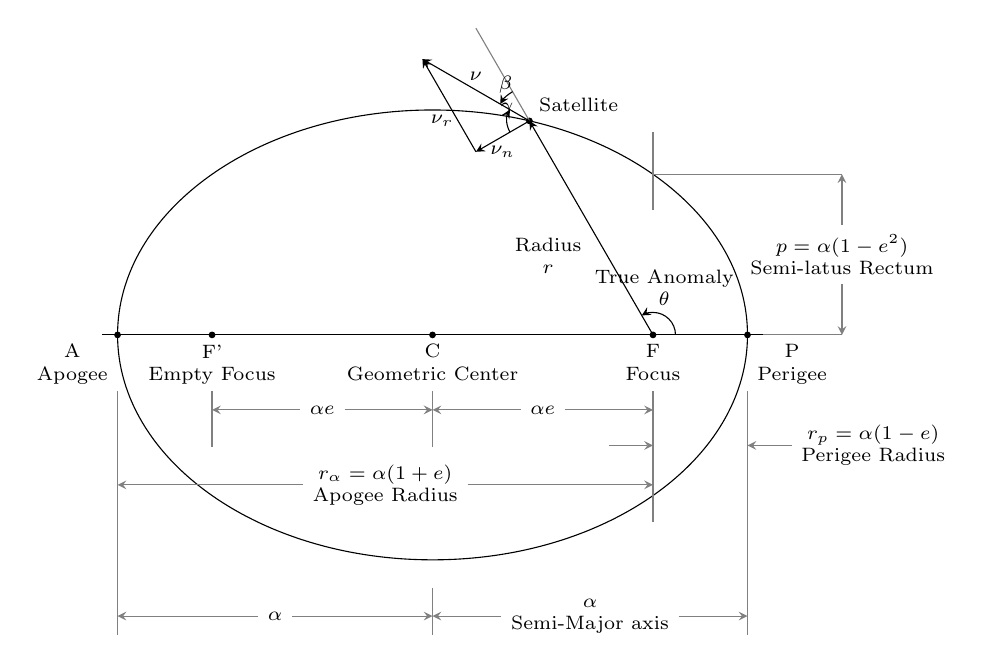
\begin{tikzpicture}
  \tikzstyle{every node}=[font=\scriptsize]
  \pgfmathsetmacro\a{4.0}
  \pgfmathsetmacro\e{0.7}
  \pgfmathsetmacro\xstart{0}
  \pgfmathsetmacro\ystart{0}
  % geometry of ellipse
  \pgfmathsetmacro\asqr{\a *\a}
  \pgfmathsetmacro\esqr{\e *\e}
  \pgfmathsetmacro\b{{\a * sqrt(1.0 - \e * \e)}}
  \pgfmathsetmacro\bsqr{\b *\b}
  \pgfmathsetmacro\c{{sqrt(\asqr - \bsqr)}}
  % coordinates of center
  \pgfmathsetmacro\xc{{\xstart - \a *cos(0)}}
  \pgfmathsetmacro\yc{{\ystart - \a *sin(0)}}
  % focal point (aka earth)
  \pgfmathsetmacro\xe{\xc + \c }
  \pgfmathsetmacro\ye{\yc }
  % left focal point
  \pgfmathsetmacro\xf{\xc - \c }
  \pgfmathsetmacro\yf{\yc }
  % true anomaly
  \pgfmathsetmacro\v{120}
  % point on ellipse, satellite
  \pgfmathsetmacro\vr{{\v}}
  \pgfmathsetmacro\p{{\a * (1e0 - \e * \e )}}
  \pgfmathsetmacro\r{{\p / (1+\e*cos(\v))}}
  \pgfmathsetmacro\xsat{{\r * cos(\v) - \xc}}
  \pgfmathsetmacro\ysat{{\r * sin(\v ) - \yc}}
  % semilatus rectum
  \pgfmathsetmacro\vsr{{90}}
  \pgfmathsetmacro\xsr{\xe}
  \pgfmathsetmacro\xsrq{{\xsr - \xc}}
  \pgfmathsetmacro\ysr{{\b *sqrt(1-(\xsrq *\xsrq)/\asqr) -\yc}}

  % mark perigee
  \node[] (perigee) 
    at ( \xstart , \ystart )
    {};
  \draw[fill=black] (perigee) circle[radius=1pt];
  \node[anchor=north west,align=center] () at (perigee){P\\Perigee};
  
  % mark empty focal point
  \node[] (empty-focal) 
    at ( \xf , \yf )
    {};
  \draw[fill=black] (empty-focal) circle[radius=1pt];
  \node[anchor=north,align=center] () at (empty-focal){F'\\Empty Focus};
  
  % mark earth
  \node[] (earth)
    at ( \xe , \ye )
    {};
  \draw[fill=black] (earth) circle[radius=1pt];
  \node[anchor=north,align=center] () at (earth){F\\Focus};
  
  % center
  \node[] (center) at (\xc , \yc ) {};
  \draw[fill=black] (center) circle[radius=1pt];
  \node[anchor=north, align=center] () at (center){C\\Geometric Center};

  % mark apogee
  \node[] (apogee) 
    at ({\xstart - \a *cos(0)+ \a *cos(180)}, {\ystart - \a *sin(0)+ \a *sin(180)})
    {};
  \draw[fill=black] (apogee) circle[radius=1pt];
  \node[anchor=north east, align=center] () at (apogee){A\\Apogee};
  
  % ellipse arc
  \draw[] ( \xstart , \ystart ) arc(0:360:\a cm and \b cm);
  
  % x-axis
  \draw[] ($(apogee) - (.2,0)$)  -- ($(perigee)+(.2,0)$);

  % true anomaly (coordinate system centered at F/Earth)
  \pgfmathsetmacro\xsat{{\xe - \r * cos(180 -\v)}}
  \pgfmathsetmacro\ysat{{\ye + \r * sin(180 -\v )}}
  \coordinate (Shift) at (\xe,\ye,0);
  \tdplotsetrotatedcoordsorigin{(Shift)}
  \draw[tdplot_rotated_coords,black,-stealth] (0,0) -- ++(\v:\r) node[midway,below left,align=center] {Radius\\$r$};
  \node[anchor=south west] () at (\xsat, \ysat) {Satellite};
  \draw[tdplot_rotated_coords,fill=black] (\v:\r) circle[radius=1pt];
  \tdplotdrawarc[tdplot_rotated_coords,-stealth]
        {(Shift)}{0.1*\b}{0}{\v}{anchor=south,align=center}{True Anomaly\\$\theta$};

  % semilatus rectum
  \draw[gray,thin] ($(perigee)+(.2,0)$) -- ($(perigee)+(.2,0)+(1.0,0)$);
  \draw[gray,thin] ($(\xe,\ye)+(0,\b/1.8)$) -- ($(\xe,\ye)+(0,\b-\b/10)$);
  \draw[gray,thin] ($(\xsr,\ysr)$) -- ($(perigee)+(.2,0)+(1.0,0)+(0,\ysr)$);
  \path ($(perigee)+(.2,0)+(1.0,0)+(0,\ysr)$) 
    -- node[align=center](semirec){$p=\alpha (1-e^2)$\\Semi-latus Rectum}
    ($(perigee)+(.2,0)+(1.0,0)$);
  \draw[gray,stealth-] ($(\xstart,\ysr)+(.2,0)+(1.0,0)$) -- (semirec);
  \draw[gray,-stealth] (semirec) -- ($(perigee)+(.2,0)+(1.0,0)$);

  % satellite velocity
  \pgfmathsetmacro\gfa{60} % angle gamma
  \pgfmathsetmacro\bfa{90-\gfa} % angle beta
  \pgfmathsetmacro\vel{{\r / 2}}
  \pgfmathsetmacro\velx{{cos(\gfa) * \vel}}
  \pgfmathsetmacro\vely{{sin(\gfa) * \vel}}
  \coordinate (Shift) at (\xsat,\ysat);
  \tdplotsetrotatedcoordsorigin{(Shift)}
  \draw[tdplot_rotated_coords,gray,thin] (0,0) -- ++(\v:\vely);
  \draw[tdplot_rotated_coords,black,-stealth] (0,0) -- ++(\v + \bfa : \vel) node[midway,above]{$\nu$};
  \draw[tdplot_rotated_coords,black,thin,-stealth] (0,0) -- ++(\v+90:\velx) node[midway,below] {$\nu _n$};
  \tdplotsetrotatedcoordsorigin{($(Shift)+(\v+90:\velx)$)}
  \draw[tdplot_rotated_coords,black,thin,-stealth] (0,0) -- ++(\v:\vely) node[midway,below,xshift=-0.6ex] {$\nu _r$};
  \tdplotdrawarc[tdplot_rotated_coords,-stealth]
        {(Shift)}{0.1*\b}{\v+90}{\v+90-\gfa}{anchor=center,yshift=1ex}{$\gamma$};
  \tdplotdrawarc[tdplot_rotated_coords,-stealth]
        {(Shift)}{0.15*\b}{\v}{\v+\bfa}{anchor=center,yshift=1.0ex}{$\beta$};


  % lower part dimensioning
  % -----------------------
  \pgfmathsetmacro\ygoff{{-\b / 4}}

  % semi-major axis
  \pgfmathsetmacro\ydaoff{{-\b -\b / 4}}
  \draw[gray,thin] ($(apogee) +  (0, \ygoff)$) 
    -- ($(apogee) +  (0, -\b -\b / 3)$);
  \draw[gray,thin] ($(perigee) + (0, \ygoff)$) 
    -- ($(perigee) + (0, -\b -\b / 3)$);
  \draw[gray,thin] ($(center) +  (0, -\b -\b / 8)$) 
    -- ($(center) + (0, -\b -\b / 3)$);
  \path ($(apogee) +  (0, \ydaoff)$) 
    --node[](alphaleft){$\alpha$} ($(center) + (0, \ydaoff)$);
  \draw[gray,thin,stealth-] ($(apogee) +  (0, \ydaoff)$) -- (alphaleft);
  \draw[gray,thin,-stealth] (alphaleft) -- ($(center) + (0, -\b \ygoff)$);
  \path ($(center) +  (0, \ydaoff)$) 
    -- node[align = center](alpharight){$\alpha$\\Semi-Major axis}
      ($(perigee) + (0, \ydaoff)$);
  \draw[gray,thin,stealth-] ($(center) +  (0, \ydaoff)$) -- (alpharight);
  \draw[gray,thin,-stealth] (alpharight) -- ($(perigee) + (0, \ydaoff)$);
  
  % apogee radius
  \pgfmathsetmacro\ydaroff{{-\b / 1.5}}
  \draw[gray,thin] ($(\xe,\ye) +  (0, \ygoff)$) 
    -- ($(\xe,\ye) +  (0, -\b / 1.2)$);
  \path ($(apogee)+(0,\ydaroff)$)
    -- node[align = center](apogeeradius){$r_\alpha =\alpha (1+e)$\\Apogee Radius}
     ($(\xe,\ye)+(0,\ydaroff)$);
  \draw[gray,stealth-] ($(apogee)+(0,\ydaroff)$) -- (apogeeradius);
  \draw[gray,-stealth] (apogeeradius) -- ($(\xe,\ye)+(0,\ydaroff)$);
  % perigee radius
  \draw[gray, thin, -stealth] ($(\xe,\ye) + (- \a * \e / 5, \ydaroff + \a /8)$) -- ($(\xe, \ye) + (0,\ydaroff + \a /8)$);
  \draw[gray, thin, -stealth] ($(perigee) + (\a * \e / 5, \ydaroff + \a /8)$) -- ($(perigee) + (0, \ydaroff + \a /8)$);
  %\path ($(\xe, \ye) + (0,\ydaroff + \a /8)$)
  %  -- node[align = center](perigeeradius){$r_p =\alpha (1-e)$\\Perigee Radius}
  %  ($(perigee) + (0, \ydaroff + \a /8)$);
  \node[anchor = west, align=center] () at ($(perigee) + (\a * \e / 5, \ydaroff + \a /8)$)
    {$r_p =\alpha (1-e)$\\Perigee Radius};

  % to foci
  \pgfmathsetmacro\ydaroff{{-\b / 3}}
  \draw[gray,thin] ($(\xf,\yf) +  (0, \ygoff)$)
    -- ($(\xf,\yf) +  (0, -\b / 2)$);
  \path ($(\xf,\yf) +  (0, \ydaroff)$) --node[](aeleft){$\alpha e$}($(\xc,\yc) +  (0, \ydaroff)$);
  \draw[gray,thin,stealth-] ($(\xf,\yf)+(0,\ydaroff)$) -- (aeleft);
  \draw[gray,thin,-stealth] (aeleft) -- ($(\xc,\yc) +  (0, \ydaroff)$);
  \draw[gray,thin] ($(\xc,\yc) +  (0, \ygoff)$)
    -- ($(\xc,\yc) +  (0, -\b / 2)$);
  \path ($(\xc,\yc) +  (0, \ydaroff)$) --node[](aeright){$\alpha e$}($(\xe,\ye) +  (0, \ydaroff)$);
  \draw[gray,thin,stealth-] ($(\xc,\yc)+(0,\ydaroff)$) -- (aeright);
  \draw[gray,thin,-stealth] (aeright) -- ($(\xe,\ye) +  (0, \ydaroff)$);
  
\end{tikzpicture}

\caption{Ellipse geometry (\cite{chobotov})}
\label{fig:ellipse-geometry}
\end{figure}
\fi

    \subsection{Orbital Elements}\label{ssec:orbital-elements}

A total of six independent parameters are needed to unambiguously define an 
arbitrary and unperturbed orbit at some instant $t$ in time. Two parameters, 
eccentricity $e$ and angular momentum $h$ (or alternatively the semi-major axis, 
$\alpha$) define the form of the orbit. To locate a point on the orbit we need a 
third parameter, the true anomaly $\theta$. Describing the orientation of the 
orbit in three dimensions requires three additional parameters, inclination $i$, 
argument of perigee $\omega$ and right ascension of the ascending node, $\Omega$. 
These six parameters are called the \emph{orbital} or 
\emph{Keplerian elements}\footnote{There exist alternate sets of (six) parameters 
that can uniquely define the orbit, but this set is by far the most widely used 
in celestial mechanics.} (see \autoref{fig:orbital-elements-3d} and 
\autoref{fig:orbital-elements-Ooi}).
\begin{description}[labelindent=1cm]
  \item[$\alpha$]: the \emph{semi-major axis} (sometimes $h$, the specific 
    \emph{angular momentum} is used instead),
  \item[$i$]: \emph{inclination},
  \item[$\Omega$]: \emph{right ascension of the ascending node},
  \item[$e$]: \emph{eccentricity},
  \item[$\omega$]: \emph{argument of perigee},
  \item[$\theta$]\footnote{True anomaly is often designated with the letter 
    $\nu$ of $f$, but here we are following the notation $\theta$}.: 
    \emph{true anomaly} (sometimes $\bm{M}$, the \emph{mean anomaly} 
    is used instead)
\end{description}

\begin{figure}
  \centering
  %% see https://tex.stackexchange.com/questions/386030/how-to-draw-orbital-elements
\tdplotsetmaincoords{70}{110}
\begin{tikzpicture}[tdplot_main_coords,scale=5]
  \pgfmathsetmacro{\r}{.8}
  \pgfmathsetmacro{\O}{45} % right ascension of ascending node [deg]
  \pgfmathsetmacro{\i}{30} % inclination [deg]
  \pgfmathsetmacro{\f}{35} % true anomaly [deg]

  \coordinate (O) at (0,0,0);
  
  % rotate and plot orbital plane (so that the ecliptic goes above it)
  \tdplotsetrotatedcoords{-\O}{\i}{0};
  \tdplotdrawarc [tdplot_rotated_coords,fill opacity=0.8,fill=red!20]
    {(O)}{\r}{0}{360}{}{};

  % rotate back and plot the ecliptic RF
  \tdplotsetrotatedcoords{\O}{-\i}{0};
  \node at (0,-\r,0) [left,text width=4em] {Ecliptic Plane}; % name of plane
  \tdplotdrawarc [dashed,fill=gray!10,fill opacity=0.9]
    {(O)}{\r}{0}{360}{}{}; % draw plane and fill it
  \draw [] (O) -- (\r,0,0); % x-axis, solid part
  \draw [-stealth,dashed] (\r,0,0) -- (2*\r + \r /2,0,0) 
    node[anchor=north east] {$\bm{x} (\aries)$}; % x-axis, dashed part
  \draw [-stealth] (O) -- (0,\r,0) node[anchor=north west] {$\bm{y}$};
  \draw [-stealth] (O) -- (0,0,\r) node[anchor=south] {$\bm{z}$};
  
  % rotate and plot the line of nodes
  \tdplotsetrotatedcoords{\O}{0}{0};
  \draw [tdplot_rotated_coords] (-1,0,0) -- (1,0,0) 
    node [below right] {Line of Nodes};
  \tdplotdrawarc[thick,-stealth]{(O)}{.33*\r}
    {0}{\O}{anchor=north}{$\bm{\Omega}$} % Omega angle

  % rotate back and plot the orbital RF
  \tdplotsetrotatedcoords{-\O}{\i}{0};
  % re-plot the part of the orbital plane above the ecliptic
  \tdplotdrawarc [tdplot_rotated_coords,fill opacity=0.8,fill=red!20]
    {(O)}{\r}{90}{270}{}{};
  \begin{scope}[tdplot_rotated_coords]
    \draw[red,-stealth] (O) -- (0,0,\r) node [above] {$\hat{\bm{h}}$};
    \tdplotdrawarc[thick,-stealth,red]{(O)}{.33*\r}{90}{180}
      {anchor=west}{$\bm{\omega}$};
    \coordinate (Sat) at (180+\f:\r);
    \draw [-stealth] (O) -- (Sat);
    \filldraw [black] (Sat) circle (0.5pt) node[anchor=south west]{Sat};
    \tdplotdrawarc[thick,-stealth,red]{(O)}{.33*\r}{180}{180+\f}
      {anchor=south west}{$\bm{\theta}$};
    \draw [thick] (O) -- (-\r,0,0) node[anchor=south west]{Periapsis/Perigee} ;
  \end{scope}
 
  % inclination ....
  \pgfmathsetmacro\ANx{\r * cos(\O)}   
  \pgfmathsetmacro\ANy{\r * sin(\O)}   
  \coordinate (Shift) at (\ANx,\ANy,0);
  \tdplotsetrotatedcoordsorigin{(Shift)};
  \tdplotsetrotatedcoords{180}{90}{180+\O)};
  %\begin{scope}[tdplot_rotated_coords]
  %\draw [tdplot_rotated_coords,blue] (0,0,0) -- (\r,0,0) node{xx};
  %\draw [tdplot_rotated_coords,blue] (0,0,0) -- (0,\r,0) node{yy};
  %\draw [tdplot_rotated_coords,blue] (0,0,0) -- (0,0,\r) node{zz};
  %\draw [tdplot_rotated_coords,black] (\r,0,0) circle (0.5pt) node[anchor=south west]{(r,0,0)};
  \tdplotdrawarc[tdplot_rotated_coords,thick,stealth-,black]
    {(Shift)}{0.2*\r}{0}{\i}{anchor=west}{$\bm{i}$};
  %\end{scope}

\end{tikzpicture}

  \caption{Geometry of orbital elements.}
  \label{fig:orbital-elements-3d}
\end{figure}

$\Omega$, $\omega$ and $i$, which define the orientation of the orbit in space, 
are sometimes called \emph{Euler angles}. Given these six elements, it is always 
possible to uniquely calculate the \emph{state vector}, that is the three spatial 
dimensions defining the position $\begin{pmatrix}x&y&z\end{pmatrix}$ in a Cartesian 
coordinate system, and their corresponding velocities 
$\begin{pmatrix}\dot{x}&\dot{y}&\dot{z}\end{pmatrix}$.

\begin{figure}
  \centering
  %% https://tex.stackexchange.com/questions/386030/how-to-draw-orbital-elements
\def\r{3.5}
\pgfmathsetmacro{\inclination}{35}
\pgfmathsetmacro{\nuSatellite}{55}
\pgfmathsetmacro{\OmegaAngle}{-290}
\pgfmathsetmacro{\omegaSatellite}{90}

\tdplotsetmaincoords{70}{165}
\begin{tikzpicture}[tdplot_main_coords]

    % Earth
    \fill (0,0) coordinate (O) circle (3pt) node[left=7pt] {$M_\oplus$};
            
    % Draw equatorial plane
    \draw[] (0,-\r,0) -- 
        (\r,-\r,0) node[below]{Equatorial plane} -- 
        (\r,\r,0) -- 
        (-\r,\r,0) -- 
        (-\r,-0.65*\r,0) ;
    \draw[dotted] (-\r,-0.65*\r,0) -- 
        (-\r,-\r,0) -- 
        (0,-\r,0);
            
    % Draw Line of nodes
    \draw[dashed] 
      (0,-1.3*\r,0) -- (0,1.4*\r,0) node[right] {Line of nodes};

    % Draw Equinox line
    \tdplotsetcoord{V}{2.0*\r}{90}{\OmegaAngle};
    \draw[->] (0,0,0) -- (V) node[anchor=west] {Vernal Equinox (\aries)};

    % Draw Omega angle
    \tdplotresetrotatedcoordsorigin
    \tdplotsetrotatedcoords{0}{0}{180}
    \tdplotdrawarc[tdplot_rotated_coords,thick,-stealth,black]
      {(0,0,0)}{0.6*\r}{250}{270}
      {anchor=north}{$\boldsymbol\Omega$};

    % Draw orbital ellipse
    \tdplotsetrotatedcoords{0}{\inclination}{90}
    \tdplotdrawarc[tdplot_rotated_coords,thin,blue]
      {(0,0,0)}{\r}{-125}{180}
      {label={[xshift=-5.7cm, yshift=-2.2cm]Orbital plane}}{}
    \tdplotdrawarc[tdplot_rotated_coords,dotted,blue]
    {(0,0,0)}{\r}{180}{235}
    {}{}

    % Draw satellite on orbital plane
    \tdplotsetrotatedcoords{0}{\inclination}{90};
    \pgfmathsetmacro{\omegaSatellite}{90}
    \pgfmathsetmacro{\xmRot}{\r*cos(\omegaSatellite+\nuSatellite)}
    \pgfmathsetmacro{\ymRot}{\r*sin(\omegaSatellite+\nuSatellite)}
    \pgfmathsetmacro{\zmRot}{0}
    \draw[tdplot_rotated_coords,thin,->,blue] 
      (0,0,0) -- (\xmRot,\ymRot,\zmRot);
    \filldraw[tdplot_rotated_coords, blue] 
      (\xmRot,\ymRot,\zmRot) circle (2pt) node[above left] {$sat$};

    % Draw periapsis line
    \draw[dashed,tdplot_rotated_coords,blue] 
      (0,0,0) -- (0,\r,0) node[anchor=south west] {Periapsis};

    % Draw omega angle
    \tdplotdrawarc[tdplot_rotated_coords,thick,-stealth,blue]
        {(0,0,0)}{0.4*\r}{0}{\omegaSatellite}
        {anchor=south west}{$\boldsymbol\omega$};

    % Draw v angle (true anomaly)
    \tdplotdrawarc[tdplot_rotated_coords,thick,-stealth,blue]
      {(0,0,0)}{0.4*\r}{\omegaSatellite}{\omegaSatellite+\nuSatellite}
      {anchor=south west}{v};

    % Draw inclination angle
    \tdplotresetrotatedcoordsorigin
    \tdplotsetrotatedcoords{0}{0}{180}
    \coordinate (Shift) at (0,\r,0);
    \tdplotsetrotatedcoordsorigin{(Shift)}
    \tdplotsetrotatedthetaplanecoords{0};
    \tdplotdrawarc[tdplot_rotated_coords,thick,-stealth,brown]
        {(Shift)}{0.3*\r}{90}{90-\inclination}{anchor=west}{$\bm{i}$}

\end{tikzpicture}

  \caption{Orbital Elements $\Omega$, $\omega$ and $i$}
  \label{fig:orbital-elements-Ooi}
\end{figure}

A real orbit and its elements change over time due to various perturbations (see 
\autoref{ssec:perturbed-motion}). A Kepler orbit is an idealized, mathematical 
approximation of the orbit at a particular time. To avoid confusion, we are going 
to adopt the distinction of orbital elements sets proposed by \cite{Vallado2001} and 
distinguish between the following cases:
\begin{description}
  \item \emph{two-body elements} are the elements derived from or used with 
    the two-body equations of motion,
  \item \emph{osculating elements} are the \emph{instantaneous} elements, under 
    the influence of perturbations, and
  \item \emph{mean elements} are the elements obtained when averaging the 
    effect of perturbations over a specified time interval
\end{description}

Mathematical formulae to transform between state vector and orbital elements can 
be found in relevant literature. In the software developed for this Thesis, the 
methodology described in \cite{Montenbruck2000} is adopted and implemented.

    \subsection{Non-Keplerian Motion}
\label{ssec:non-keplerian}

The two-body problem (\ref{ssec:two-body-problem}) is the basis for most 
trajectory problems, due to (\cite{hintz}):
\begin{enumerate}
  \item the relative two-body problem can be solved analytically,
  \item it is often a good approximation to the real solution (central body 
    gravitational force is dominant compared to perurbing forces),
  \item provides a clear and illustritive picture of the situation, and
  \item it can be used as a reference trajectory for precise orbit 
    determination techniques
\end{enumerate}

In the framework of Newtonian physics, the motion of a satellite under the influence 
of a force $\bm{F}$ is described by the differential equation (\cite{Montenbruck2000})
\begin{equation}
  \bm{\ddot{r}} = \frac{\bm{F} (t, \bm{r}, \bm{v})}{m}
\end{equation}
in a \emph{non-rotating} reference system ($m$ being the satellite's mass).
In the \ref{ssec:two-body-problem}, we consider only the gravitational force 
\ref{eq:mont32}, assuming point masses or a radially symmetric force, obtaining 
an elliptic satellite orbit with fixed orbital plane.

In real world, satellite orbits are \emph{perturbed} away from Keplerian 
orbits, due to forces other than the central body's gravitational force, i.e. 
other than those that cause it to move along a reference trajectory.

A perturbing force is \emph{conservative}\footnote{
A force field $\bm{F}$ is is called a conservative force if it meets one of the 
following three demands:
  \begin{enumerate}
    \item the \emph{curl} of $\bm{F}$ is zero:\begin{equation}\vec{\nabla} \times \bm{F} = \bm{0}\end{equation}
    \item there is zero net work done by the force when moving a particle 
      through a loop trajectory:\begin{equation}W \equiv \oint _C \bm{F}d\bm{r}=0 \end{equation}
    \item the force can be written as the gradient of a potential:\begin{equation}\bm{F}=-\vec{\nabla} U\end{equation}
  \end{enumerate}
  } if it is derivable from a scalar 
function:
\begin{equation}
  \bm{F} = -\nabla U(\bm{r})
\end{equation}

The perturbing forces caused by third bodies are conservative field forces. 
There are also non-conservative perturbing forces such as atmospheric drag.

In the following, we are going to discuss the \emph{Force Model} acting on an 
Earth orbiting satellite.

      \subsubsection{Geopotential}\label{sssec:geopotential}

In the two-body problem (\autoref{ssec:two-body-problem}) a radially symmetric 
gravity force was assumed, acting like a point mass. For \gls{pod} however, this 
assumption needs to be replaced by a model closer to a real world scenario.
As known, the Earth is not a perfect sphere, but rather resembles an oblate spheroid, 
with different equatorial and polar diameter. To derive a more realistic model, 
it is convenient to use an equivalent representation involving the gradient of 
the corresponding gravity potential $U$ (\cite{Montenbruck2000}):
\begin{equation}
  \label{eq:geopotential}
  \ddot{\bm{r}} = \nabla U \textrm{ where } U = G M_{\Earth} \frac{1}{r}
\end{equation}
so that 
$\bm{F} = \begin{pmatrix} \frac{\partial U}{\partial x} & \frac{\partial U}{\partial y} & \frac{\partial U}{\partial z} \end{pmatrix}$
This formulation enables the replacement of the three components of the vector 
$\bm{F}$ by a single function $U$, thus simplifying notation and further 
developments. The geopotential is widely used in geodesy (see e.g. \cite{Moritz2005}).

Given an arbitrary mass distribution, the individual elementary mass contributions 
$dm = \rho (\bm{s}) d^3 s$ can be summed, and thus the potential be expressed as:
\begin{equation}\label{eq:mont34}
  U = G \int \frac{\rho (\bm{s})}{\norm{\bm{r}-\bm{s}}} \, d^3 s
\end{equation}
where $\bm{r}$ is the vector from the mass center to the attracted body (i.e. satellite) 
and $\bm{s}$ is the geocentric vector the elementary mass $dm$.

For any point $\bm{r}$ outside the mass, $r > s$, the inverse of the distance can 
be expanded using a series of \emph{Legendre polynomials}, as
\begin{equation}
  \frac{1}{\norm{\bm{r}-\bm{s}}} = \frac{1}{r} \sum_{n=0}^{\infty} 
    \left( \frac{s}{r} \right) ^n  P_n ( \cos \gamma )
\end{equation}
where $\cos \gamma = \frac{\bm{r} \cdot \bm{s}}{rs}$ (the angle between $\bm{r}$
and $\bm{s}$) and $P_n(u)$ is the Legendre polynomial of degree $n$. Making use of 
the addition theorem of Legendre polynomials (\cite{Montenbruck2000}):
\begin{equation}
  \label{eq:mont38}
  P_n (\cos \gamma ) = \sum_{m=0}^{n} \left( 2 - \delta _{0m} \right) 
    P_{nm} (\sin \phi ) P_{nm} (\sin{\phi ^\prime}) 
    \cos{m \left( \lambda - \lambda ^\prime \right) }
\end{equation}
with $P_{nm}$ the \emph{associated Legendre polynomials} of degree $n$ and order 
$m$ and $\begin{pmatrix} \phi & \lambda \end{pmatrix}$ and 
$\begin{pmatrix} \phi ^\prime & \lambda ^\prime \end{pmatrix}$ being the longitude 
and geocentric latitudes of points $\bm{r}$ and $\bm{s}$ respectively.

The Earth's gravity potential can now be written as:
\begin{equation}\label{eq:mont310}
  U (r, \phi, \lambda ) = \frac{G M_{\Earth}}{r} \sum_{n=0}^{\infty} \sum_{m=0}^{n} 
      \left( \frac{R_{\Earth}}{r} \right) ^n P_{nm} (\sin \phi )
      \left( C_{nm} \cos {m\lambda} + S_{nm} \sin{m\lambda} \right)
\end{equation}
with coefficients:
\begin{equation}
  \begin{aligned}
    C_{nm} = \frac{2 - \delta _{0m}}{M_{\Earth}} \frac{(n-m)!}{(n+m)!} 
      \int \left({\frac{s}{R_{\Earth}}}\right)^n P_{nm} (\sin \phi ^\prime) \cos {m\lambda ^\prime} \rho (\bm{s}) \, d^3 s \\
    S_{nm} = \frac{2 - \delta _{0m}}{M_{\Earth}} \frac{(n-m)!}{(n+m)!} 
      \int \left({\frac{s}{R_{\Earth}}}\right)^n P_{nm} (\sin \phi ^\prime) \sin {m\lambda ^\prime} \rho (\bm{s}) \, d^3 s
  \end{aligned}
\end{equation}
which describe the dependence on the Earth's internal mass distribution. In geodetic 
applications, the \emph{normalized} geopotential coefficients $\bar{C}_{nm}$ and 
${\bar{S}}_{nm}$, are most often used, and defined as
\begin{equation}
  \begin{Bmatrix} \bar{C}_{nm} \\ \bar{S}_{nm} \end{Bmatrix} = 
  \sqrt{\frac{(n+m)!}{\left(2-\delta _{0m}\right) \left(2n+1\right) \left(n-m\right)!}}
  \begin{Bmatrix} C_{nm} \\ S_{nm} \end{Bmatrix}
\end{equation}
which are much more uniform in magnitude, thus helping reduce round-off errors.
Note that the coefficients $C_{nm}$ and $S_{nm}$ are often called 
\emph{Stokes' coefficients}, e.g. \cite{Barthelmes2018}.

The acceleration due to the Earth's gravity potential can now be written as  
(\cite{Montenbruck2000})
\begin{equation}\label{eq:mont315}
  \bm{\ddot{r}} (r, \phi, \lambda ) = \nabla \frac{GM_{\Earth}}{r} \sum_{n=0}^{\infty} \sum_{m=0}^{n} 
    \left(\frac{R_{\Earth}}{r}\right) ^n \bar{P}_{nm} (\sin \phi )
    \left( \bar{C}_{nm} \cos{m\lambda} + \bar{S}_{nm} \sin{m\lambda} \right)
\end{equation}
where the \emph{normalized} associated Legendre functions are used
\begin{equation}
  \bar{P}_{nm} = \sqrt{\frac{\left(2-\delta _{0m}\right) \left(2n+1\right) \left(n-m\right)!}{(n+m)!}} P_{nm}
\end{equation}

\paragraph{Gravity Models}\label{par:gravity-models}

Earth gravity models, contain the potential coefficients $\bar{C}_{nm}$ and $\bar{S}_{nm}$ 
up to a given degree $n$ and order $m$ (with $m \le n$) and the parameters $GM_{\Earth}$ 
and $R_{\Earth}$ via which one can compute the geopotential or the induced acceleration 
on an orbiting satellite, given its position vector $\bm{r}$. Gravity models are derived from:
\begin{description}
  \item[Satellite data], making use of the fact that the Earth's gravity field 
    can produce perturbations ``seen'' in satellite orbits via \gls{pod}. It is worth 
    noting that since \gls{grace} (\cite{Tapley2004b}) was launched in March 2002, satellite 
    gravimetry has brought a new era of studying global mass variation and redistribution 
    through measuring the time-variable gravity field with unprecedented accuracy 
    (see e.g. \cite{Chen2022} and \cite{Jaggi2023}). This progress was further enhanced 
    with the launch of \gls{goce} (\cite{Johannessen2003}) in 2009.
  \item[Terrestrial observations] (surface gravimetry), providing precise local 
    and regional (short-wavelength) information on the gravity field. Due to their 
    inhomogeneous distribution though, deriving a global gravity model is quite challenging.
  \item[Altimeter data], which provide detailed information about the form of the 
    geoid, which may in turn be used to derive geopotential coefficients.
  \item[Combinations] of the above methods/data.
\end{description}

Recent advantages in gravity models and estimation, have enabled temporal modeling 
of the geopotential coefficients. Thus, the parameters $\bar{C}_{nm}$ and 
$\bar{S}_{nm}$ are not constant but slightly varying with time. Most often, the 
parametrization of the coefficients consists of two parts, 
\begin{itemize}
  \item a \emph{linear} part, including terms for a ``bias'' and a drift coefficient, pertaining 
    to a given validity interval; normally, the bias and drift are in general coherent 
    so that the result is a piece wise linear function, except in the case of earthquakes.
    E.g., for the case of \emph{CNES/GRGS RL04} (\cite{Lemoine2019}), three major 
    earthquakes have been introduced in the modelling: Sumatra on 2004/12/26, Concepcion 
    on 2010/02/27 and Sendai on 2011/03/11.
  \item a \emph{harmonic} part, usually including two annual and two semi-annual 
    coefficients for each year (in- and out-of-phase).
\end{itemize}

In these \gls{tvg} models, the normalized Stoke's coefficients are given by:
\begin{equation}\label{eq:tvg-stokes}
  \begin{aligned}
    \bar{C}_{nm} (t) = \bar{C}_{nm}\at{t_0,k} + V_{\bar{C}_{nm},k} \cdot (t-t_0) + 
      \sum_{j=0}^{N} \left( A_{\bar{C}_{nm},j} \sin \left( \frac{2\pi}{T} \delta t \right)
      + B_{\bar{C}_{nm},j} \cos \left( \frac{2\pi}{T} \delta t \right) \right) \\
    \bar{S}_{nm} (t) = \bar{S}_{nm}\at{t_0,k} + V_{\bar{S}_{nm},k} \cdot (t-t_0) + 
      \sum_{j=0}^{N} \left( A_{\bar{S}_{nm},j} \sin \left( \frac{2\pi}{T} \delta t \right)
      + B_{\bar{S}_{nm},j} \cos \left( \frac{2\pi}{T} \delta t \right) \right)
  \end{aligned}
\end{equation}
for each validity interval $k$ valid within the period $t_{start}, t_{end}$, 
where $t_{start} < t < t_{end}$ and
\begin{description}
  \item $\bar{C}_{nm}\at{t_0}$ and $\bar{S}_{nm}\at{t_0}$ are the constant, ``bias'' 
    terms for the given interval and degree/order coefficient $(n,m)$,
  \item $V_{\bar{C}_{nm}}$ and $V_{\bar{S}_{nm}}$ are the drift terms for the 
    given interval and degree/order coefficient $(n,m)$,
  \item $j$ is the number of harmonics signals (frequencies) included in the model,
  \item $A_{\bar{C}_{nm},j}$ and $A_{\bar{S}_{nm},j}$ are the in-phase amplitudes of 
    the frequency $j$, for the degree/order coefficient $(n,m)$ coefficient,
  \item $B_{\bar{C}_{nm},j}$ and $B_{\bar{S}_{nm},j}$ are the out-of-phase amplitudes of 
    the frequency $j$, for the degree/order coefficient $(n,m)$ coefficient,
  \item $t_0$ is the reference epoch for the given validity interval,
  \item $\delta t$ is the difference between the epoch $t$ and the start of the 
    current year (in years)
\end{description}

\paragraph{The \gls{icgem}}\label{par:icgem}
\gls{icgem} (\cite{icgempub}) is one of five services coordinated by the 
\gls{igfs} of the \gls{iag}. Among other services, \gls{icgem} collects and 
archives all existing global gravity field models and provides a web interface 
for getting access to them.

Gravity models are published in what is called the \emph{ICGEM-format} 
(\cite{ICGEMFormat}), an effort to standardize the distribution of such models, 
that is gaining evermore attention in recent years. This format offers great 
advantages since it is standardized, well documented, generic and can be used to 
publish and/or parse (with slight extensions) coefficients other than gravity 
models (e.g. ocean tides).

\paragraph{Implementation}\label{par:implementation}
For the purposes of the current Thesis, software has been designed and developed 
to handle the modeling of the Earth's gravity models. Highlights of the software 
are:
\begin{itemize}
  \item Handling (parsing) of gravity models published in the \emph{ICGEM-format} 
    (see \autoref{par:icgem}). This approach enables genericity, since any (recently 
    published) gravity model can be used as input to compute satellite acceleration 
    (see e.g. the listed models published in the \gls{icgem} site \url{http://icgem.gfz-potsdam.de/tom_longtime}).
    This important feature, makes the software highly suitable for scientific studies.
  \item Handling of both static and \gls{tvg} models; for the latter, the formulation 
    \autoref{eq:tvg-stokes} is used, to account for temporal modelling of the 
    Stoke's coefficients.
  \item Efficient memory handling and introduction of special data structures to 
    store and retrieve coefficients, directly targeting and exploiting their intrinsic
    characteristics (e.g. $\bar{S}_{0m}$ are not stored).
  \item Direct retrieval and usage of the data structures to compute acceleration, 
    as well as partials (i.e. $\frac{\partial \bm{\ddot{r}}}{\partial \bm{r}}$), 
    in one step.
  \item Algorithmic design to account for efficiency, yet with as close as possible 
    minimal loss of precision due to truncation errors (e.g. employ a 
    \emph{Kahan summation} algorithm, \cite{Klein2006}).
\end{itemize}

In the current Thesis, two gravity models are used, namely \emph{EIGEN-6C4} 
(\cite{Forste2014}) and \emph{CNES/GRGS RL04}. The former is mainly used for validation 
purposes (see \autoref{sssec:gravity-acceleration}). The latter is the most 
recent recommendation of the \gls{ids} (see \cite{Lemoine2019b}, \cite{Stepanek2022a}) 
used in the latest processing campaign for ITRF2020. Note though, that the software 
is designed in a generic way, allowing the introduction of any gravity field model 
structured in the \emph{ICGEM-format}.

%% -------------------------------------------------------------------- %%
\iffalse
Models for the geopotential usually describe the static part of the field. For 
precision applications, time varying effects should also be taken into account. 
According to \cite{iers2010}, these are:
\begin{itemize}
  \item secular variations of coefficients,
  \item solid Earth tides,
  \item ocean tides,
  \item solid Earth pole tide and
  \item ocean pole tide
\end{itemize}

The expression for the potential (\ref{eq:geopotential}) may easily be 
generalized to an arbitrary mass distribution by summing up the contributions 
created by individual mass elements
\(dm = \rho(\vec{s}) d^3 \vec{s}\) according to (\cite{Montenbruck2000})
\begin{equation}
    U = G \int{\frac{\rho(\vec{s}) d^3 \vec{s}}{\lvert \vec{r} - \vec{s} \rvert}}
\end{equation}

\subsection{Earth's Geopotential Models}
The geopotential field $U$ at the point $(r, \phi , \lambda )$ is expanded in 
spherical harmonics up to degree $N$, as
\begin{equation}
  \label{eq:iers201061}
  U(r, \phi , \lambda ) = \frac{G M_{\Earth}}{r} \sum_{n=0}^N 
    {\left(\frac{\alpha _e}{r}\right)}^n 
     \sum_{m=0}^n \left[ \bar{C}_{nm} \cos {m \lambda} + \bar{S}_{nm} \sin{m \lambda} \right] 
     \bar{P}_{nm}( \sin \phi )
\end{equation}
with $\bar{S}_{n0} = 0$ and $\bar{C}_{nm}$, $\bar{S}_{nm}$ the normalized
\footnote{Since the geopotential coefficients $C_{nm}$ and $S_{nm}$ span ten or 
more orders of magnitude (\cite{Montenbruck2000}), making the computation 
susceptible to overflow and round-off errors, we usually use the corresponding 
normalized values. The latter are much more uniform in magnitude, and their 
size is approximately given by the empirical \emph{Kaula rule} (see 
\cite{Montenbruck2000} and \cite{Kaula2000}):
\begin{equation} \bar{C}_{nm} , \bar{S}_{nm} \approx \frac{10^{-5}}{n^2} \end{equation}}
geopotential coefficients the normalized. $\bar{P}_{nm}$ are the normalized 
associated Legendre functions, related to the unnormalized ones by:
\begin{subequations}
  \begin{align}
    \bar{P}_{nm} &= N_{nm} P_{nm} \label{eq:iers201062a} \\
    N_{nm} &= \sqrt{\frac{(n-m)!(2n+1)(2-\delta _{0m})}{(n+m)!}} 
      \quad \delta _{0m} = 
        \begin{cases}
          1 \quad \text{ if } m = 0 \\
          0 \quad \text{ if } m \neq 0
        \end{cases}
        \label{eq:iers201062b}
  \end{align}
\end{subequations}
Correspondingly, the normalized and unnormalized geopotential coefficients are 
related by:
\begin{subequations}
  \begin{align}
    C_{nm} &= N_{nm} \bar{C}_{nm} \\
    S_{nm} &= N_{nm} \bar{S}_{nm}
  \end{align}
\end{subequations}

For all \emph{zonal} terms, we have:
\begin{equation}
  S_{n,0} = 0 \quad C_{n,0} = -J_n
\end{equation}
where we use the ``traditional'' notation $J_n$ for \emph{zonal coefficients}. 
All $S_{n0}$ coefficients vanish (due to their definition).

Coefficients for $m<n$ are known as ``\emph{tesseral}'', while when $m=n$, the 
respective coefficients are called ``\emph{sectorial}''.


\subsubsection{Static Geopotential Models}
For computations, the Earth's gravity potential at point $(r, \phi , \lambda )$
can be approximated using a spherical harmonics expansion 
(e.g. \cite{Montenbruck2000})
\begin{equation}
    U = \frac{G M_{\Earth}}{r} \sum_{n=0}^\infty \sum_{m=0}^n 
    \frac{R_{\Earth}^n}{r^n} P_{nm} \left( \sin \phi \right) 
    \left( C_{nm} \cos{m\lambda} + S_{nm} \sin{m\lambda} \right)
\end{equation}

with the coefficients \(C_{nm}\) and \(S_{nm}\) describing the dependence on the 
Earth's internal mass distribution. These coefficients can be extracted from a 
suitable geopotential model.

Note that Geopotential coefficients with \(m=0\) are called  \emph{zonal} coefficients, 
since they describe the part of the potential that does not depend on the longitude. 
All \(S_{n0}\) vanish due to their definition, and the notation \(J_n = -C_{n0}\) 
is commonly used for the remaining zonal terms. The other geopotential coefficients
are known as \emph{tesseral} and \emph{sectorial} coefficients for \(m<n\) and 
\(m = n\), respectively.

\fbox{\begin{minipage}{.9\textwidth}
To compute the acceleration \(\ddot{\vec{r}}\), which is equal to the 
gradient of \(U\), we use the recursion formulas described in \cite{Montenbruck2000}.
Note that these expressions, use the \underline{non-normalized} harmonic 
coefficients. 
\end{minipage}}

%\subsubsection{Gravity Models}
The \href{http://icgem.gfz-potsdam.de/home}{International Centre for Global Earth Models (ICGEM)}  
(\cite{icgempub}) web service hosts a large number of gravity field models, 
published in what is called the \emph{The ICGEM-format}(\cite{ICGEMFormat}). 

Such static model files can be parsed and the respective harmonic coeefficients 
(\(C_{nm}\) and \(S_{nm}\)) be used to compute satellite acceleration induced by 
the geopotential.

Practicaly, the degree and order used depends on the accuracy of the 
application and can be truncated. According to \cite{iers2010}, truncation levels 
providing a 3-dimensional orbit accuracy of better than \SI{0.5}{\mm} as a 
function of orbit radius, are listed in \ref{table:egm2008-truncation-levels} 
for EGM2008 (\cite{pavlisegm08}).

\begin{table}
\centering
\begin{tabular}{c c c}
 \hline
 Orbit radius [km] & Example Satellite & Truncation level \\
 \hline
  7331  & Starlette & 90 \\
  12270 & Lageos    & 20 \\
  26600 & GPS       & 12 \\
 \hline
\end{tabular}
\caption{Suggested truncation levels for use of EGM2008 at different orbits according to \cite{iers2010}.}
\label{table:egm2008-truncation-levels}
\end{table}
\fi

      \subsubsection{Computing Gravity Acceleration}\label{sssec:gravity-acceleration}

The acceleration of an Earth orbiting satellite due to the Earth's gravity field, 
can be computed using the potential $U$ (see \autoref{eq:geopotential})
\begin{equation}
  \bm{\ddot{r}} =  
    \begin{pmatrix} \ddot{x} & \ddot{y} & \ddot{z} \end{pmatrix} = 
    \nabla U
\end{equation}

The classical formulation of the gravitational acceleration derived from the spherical 
harmonics expansion (see \autoref{eq:mont315}) employs the geocentric spherical coordinate 
representation. This approach can result in singularities at the north and 
south poles (\cite{Atallah2022}). To avoid this problem, our implementation of the 
computation algorithm is based on a development based on Cartesian components, 
introduced by \cite{Cunningham1970} and also presented in \cite{Montenbruck2000}, 
which is singularity-free. However, the derivation and results described therein 
use the un-normalized form; an equivalent, normalized form was derived and implemented, 
taking into account \cite{Atallah2022}. In the following, we derive the algorithmic 
approach adopted in the design of the software built for the current Thesis.

If we define 
\begin{equation}
  \bar{V}_{nm} = \bar{M}_{nm} + i \bar{W}_{nm} = 
    \left( \frac{R_{\Earth}}{r} \right) ^{n+1} \bar{P}_{nm} (\sin \phi) 
      \left( \cos (m\lambda) + i \sin (m\lambda) \right)
\end{equation}

we can rewrite the potential (see \autoref{eq:mont310}), as
\begin{equation}
  U = \Re \left( \frac{GM_{\Earth}}{R_{\Earth}} \sum_{n=0}^{\infty} \sum_{m=0}^{n} 
    \left( \bar{C}_{nm} - i \bar{S}_{nm} \right) \bar{V}_{nm} \right)
\end{equation}
using normalized coefficients, so that the acceleration is given by
\begin{equation}
  \bm{\ddot{r}} = \Re \left( \frac{GM_{\Earth}}{R_{\Earth}} \sum_{n=0}^{\infty} \sum_{m=0}^{n} 
    \left( \bar{C}_{nm} - i \bar{S}_{nm} \right) \nabla \bar{V}_{nm} \right)
\end{equation}

Omitting intermediate results (see e.g. \cite{Atallah2022}), we end up in the 
recurrence relations:
\begin{equation}
  \begin{aligned}
    \bar{V}_{nm} = B_{nm} \frac{z}{r} \frac{R_{\Earth}}{r} \bar{V}_{n-1,m} 
      - (n+m-1) \frac{B_{nm}}{B_{n-1,m}} \left( \frac{R_{\Earth}}{r} \right) ^2 \bar{V}_{n-2,m} \\
    \bar{M}_{nm} = B_{nm} \frac{zR_{\Earth}}{r^2} \bar{M}_{n-1,m} 
      - \frac{B_{nm}}{B_{n-1,m}} \left( \frac{R_{\Earth}}{r} \right) ^2 \bar{M}_{n-2,m} \\
    \bar{W}_{nm} = B_{nm} \frac{zR_{\Earth}}{r^2} \bar{W}_{n-1,m} 
      - \frac{B_{nm}}{B_{n-1,m}} \left( \frac{R_{\Earth}}{r} \right) ^2 \bar{W}_{n-2,m}
  \end{aligned}
\end{equation}
where 
\begin{equation}
  B_{nm} = \sqrt{\frac{(2n+1)(2n-1)}{(n+m)(n-m)}}
\end{equation}

and for the $n=m$ cases, we have
\begin{equation}
  \begin{aligned}
    \bar{V}_{mm} &= \sqrt{\frac{2m+1}{2m}} \frac{\left(x+iy\right)}{r^2} \bar{V}_{m-1,m-1} \\
    \bar{M}_{mm} &= \sqrt{\frac{2m+1}{2m}} \left( \frac{xR_{\Earth}}{r^2} \bar{M}_{m-1,m-1} 
      - \frac{yR_{\Earth}}{r^2} \bar{W}_{m-1,m-1} \right) \\
    \bar{W}_{mm} &= \sqrt{\frac{2m+1}{2m}} \left( \frac{xR_{\Earth}}{r^2} \bar{W}_{m-1,m-1} 
      + \frac{yR_{\Earth}}{r^2} \bar{M}_{m-1,m-1} \right) \\
  \end{aligned}
\end{equation}

The recurrence starts with initial conditions
\begin{equation}
  \begin{aligned}
    \bar{M}_{00} = \frac{R_{\Earth}}{r} &\text{ and } 
      \bar{M}_{10} = \sqrt{3} \frac{z}{r^2} \bar{M}_{00} \\
    \bar{W}_{00} = 0 &\text{ and } \bar{W}_{10} = 0
  \end{aligned}
\end{equation}

Now we can use the $\bar{M}_{nm}$ and $\bar{W}_{nm}$ to compute the Cartesian acceleration 
components using
\begin{equation}
  \begin{aligned}
    \ddot{x} & = \sum_{n=0}^{\infty} \sum_{m=0}^{n} \ddot{x}_{nm} \\
    \ddot{y} & = \sum_{n=0}^{\infty} \sum_{m=0}^{n} \ddot{y}_{nm} \\
    \ddot{z} & = \sum_{n=0}^{\infty} \sum_{m=0}^{n} \ddot{z}_{nm}
  \end{aligned}
\end{equation}

where for $m=0$
\begin{equation}
  \begin{aligned}
    \ddot{x}_{n0} &= -\frac{GM_{\Earth}}{R^2_{\Earth}} \frac{N_{n,0}}{N_{n+1,1}}\bar{C}_{n0}\bar{M}_{n+1,1} \\
    \ddot{y}_{n0} &= -\frac{GM_{\Earth}}{R^2_{\Earth}} \frac{N_{n,0}}{N_{n+1,1}}\bar{C}_{n0}\bar{W}_{n+1,1} \\
    \ddot{z}_{n0} &= -\frac{GM_{\Earth}}{R^2_{\Earth}} \frac{N_{n,0}}{N_{n+1,1}} \left(n+1\right) \bar{C}_{n0}\bar{M}_{n+1,0}
  \end{aligned}
\end{equation}

and for $m > 0$
\begin{equation}
  \begin{aligned}
    \ddot{x}_{nm} &= \frac{GM_{\Earth}}{2R^2_{\Earth}} \Bigl( \frac{N_{n,m}}{N_{n+1,m+1}} 
      \left(-\bar{C}_{n,m} \bar{M}_{n+1,m+1} + \bar{S}_{n,m} \bar{W}_{n+1,m+1} \right) \\
       & +\frac{(n-m+2)!}{(n-m)!} \frac{N_{n,m}}{N_{n+1,m-1}}
        \left(-\bar{C}_{n,m} \bar{M}_{n+1,m-1} + \bar{S}_{n,m} \bar{W}_{n+1,m-1} \right) \Bigr) \\
    \ddot{y}_{nm} &= \frac{GM_{\Earth}}{2R^2_{\Earth}} \Bigl( \frac{N_{n,m}}{N_{n+1,m+1}} 
      \left(-\bar{C}_{n,m} \bar{W}_{n+1,m+1} + \bar{S}_{n,m} \bar{M}_{n+1,m+1} \right) \\
       & +\frac{(n-m+2)!}{(n-m)!} \frac{N_{n,m}}{N_{n+1,m-1}}
        \left(-\bar{C}_{n,m} \bar{W}_{n+1,m-1} + \bar{S}_{n,m} \bar{M}_{n+1,m-1} \right) \Bigr) \\
    \ddot{z}_{nm} &= \frac{GM_{\Earth}}{R^2_{\Earth}} \frac{N_{n,m}}{N_{n+1,m}} 
      \left( \left( n-m+1 \right)
      \left(-\bar{C}_{n,m} \bar{W}_{n+1,m+1} + \bar{S}_{n,m} \bar{M}_{n+1,m+1} \right) 
        \right)
  \end{aligned}
\end{equation}

where $N_{nm}$ is the normalization factor for degree $n$ and order $m$
\begin{equation}
  N_{nm} = \sqrt{ \frac{(n-m)! (2n+1) (2-\delta _{0m})}{(n+m)!} }
\end{equation}

\paragraph{Derivative of Acceleration}\label{sssec:derivative-geopotential-acceleration}

Partial derivatives of the acceleration need to be computed, with respect to the 
satellite state vector, $\frac{\partial \bm{\ddot{r}}}{\partial \bm{r}}$ for the 
variational equations. For the central term
\begin{equation}
  \bm{\ddot{r}} = - \frac{GM_{\Earth}}{r^3}\bm{r}
\end{equation}
and using the relation
\begin{equation}
  \frac{\partial r^n}{\partial \bm{r}} = 
    \frac{\partial \left(x^2 + y^2 + z^2 \right)}{\partial \bm{r}} = 
      n \cdot r^{n-2} \cdot \bm{r}^T
\end{equation}
if follows that
\begin{equation}
  \begin{aligned}
    \frac{\partial \bm{\ddot{r}}}{\partial \bm{r}} &= 
    -GM_{\Earth} \frac{\partial}{\partial \bm{r}}\left( \bm{r} \frac{1}{r^3} \right) = 
    -GM_{\Earth} \left( \frac{1}{r^3}\bm{I}_{3\times 3} - 3\bm{r} \frac{\bm{r}^T}{r^5} \right) \\
    &=\frac{-GM_{\Earth}}{{r^5}} \begin{pmatrix}
      3x^2-r^2 & 3xy      & 3xz \\
      3yx      & 3y^2-r^2 & 3yz \\
      3zx      & 3zy      & 3z^2 -r^2
    \end{pmatrix}
  \end{aligned}
\end{equation}
which shows that the gravity gradient is symmetric and with a zero trace. The same result 
can be deduced considering Earth's gravitational potential expressed as \autoref{eq:mont34} 
(see \cite{Montenbruck2000}). The two properties reduce the number of independent 
components that have to be considered in the computation from nine to five. 

Deriving the partials is quite tedious and requires analytical work. For the computation, 
we proceed on the basis of the development used in \autoref{sssec:gravity-acceleration}, 
following a normalized version of \cite{Cunningham1970} to compute the quantities 
$\frac{\partial \ddot{x}_{nm}}{\partial x}$, 
$\frac{\partial \ddot{x}_{nm}}{\partial y}$, $\frac{\partial \ddot{x}_{nm}}{\partial z}$, 
$\frac{\partial \ddot{y}_{nm}}{\partial z}$ and $\frac{\partial \ddot{z}_{nm}}{\partial z}$.

\paragraph{Earth Rotation}\label{sssec:gravity-acceleration-earth-rotation}

Formulas presented in the current section, \autoref{sssec:gravity-acceleration}, 
are valid in an \gls{ecef} frame, that is ignoring Earth's rotation (aka $\bm{r}$ is 
the satellite's position vector in \gls{ecef} coordinates). We are now designating 
the $\bm{r}$ vector as $\bm{r}_{ef}$ and introducing $\bm{r}_{sf}$ to designate the 
corresponding celestial, ``space-fixed'' vector, with 
\begin{equation}
  \bm{r}_{ef} = \bm{R} \cdot \bm{r}_{sf}
\end{equation}
where $\bm{R}$ is the terrestrial-to-celestial transformation matrix (see 
\autoref{ssec:itrs-to-gcrs}). The partial derivatives 
$\frac{\partial \bm{\ddot{r}}}{\partial \bm{r}}$ is the ``space-fixed'' 
frame, would then be given by
\begin{equation}
  \left( \frac{\partial \bm{\ddot{r}}}{\partial \bm{r}} \right) _{sf} = 
  \bm{R}^T 
  \left( \frac{\partial \bm{\ddot{r}}}{\partial \bm{r}} \right) _{ef}
  \bm{R}
\end{equation}
and for the acceleration
\begin{equation}
  \bm{\ddot{r}}_{sf} = \bm{R}^T \cdot \bm{\ddot{r}}_{ef}
\end{equation}

\paragraph{Validation}\label{sssec:gravity-acceleration-acceleration}

The acceleration induced to an earth orbiting satellite by the Earth's gravity 
field, is by far the largest in magnitude, hence it should be computed with utmost 
precision. To test the implementation, results obtained we checked against the \texttt{COST-G} 
benchmark test. Input data for the test is a one-day orbital arc of \gls{grace}, paired
with the earth gravity model \texttt{EIGEN-6C4}. Acceleration is evaluated from degree
and order 2 to 180 (i.e. leaving out the largest in magnitude central term). According 
to \cite{Lasser23}, accelerations should be consistent to at least \SI{10e-12}{\metre\per\square\second}.
The discrepancies between our implementation and the benchmark test are depicted in 
\autoref{fig:costg-benchmark-02gravityfield-itrf} and \autoref{table:costg-benchmark-02gravityfield-itrf}. 
It is clear that results obtained lie within the accuracy demands of the benchmark test.

\begin{figure}
  \centering
  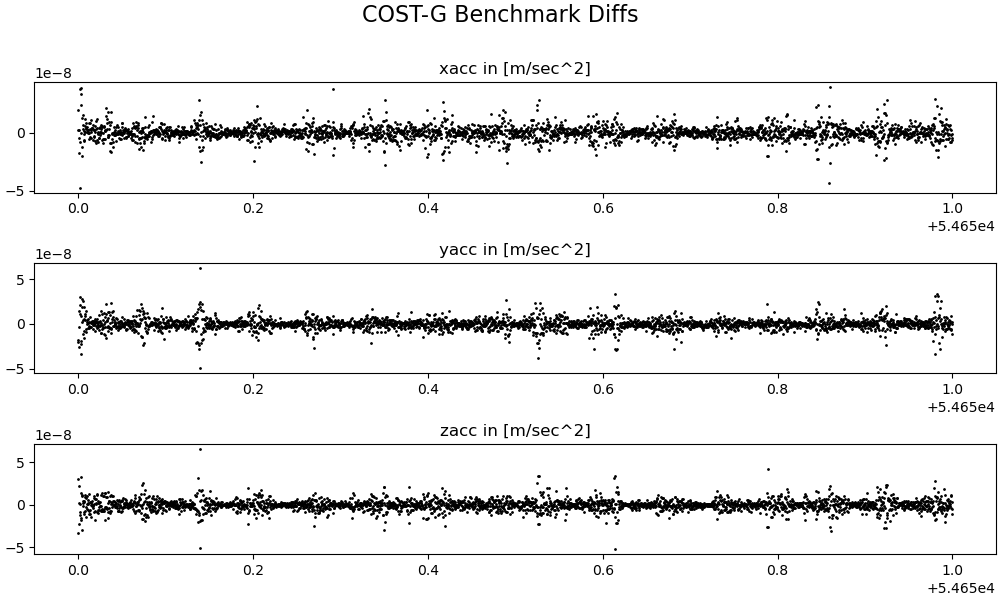
\includegraphics[height=.4\textheight,keepaspectratio]{02gravityfield_itrf}
  \caption{Earth gravity acceleration discrepancies against the \texttt{COST-G} 
    benchmark test. Gravity model is \texttt{EIGEN-6C4} from degree and order 2 to 180. 
    Comparing results for a one-day orbit arc of \gls{grace} in \gls{itrf}.}
  \label{fig:costg-benchmark-02gravityfield-itrf}
\end{figure}

\begin{table}[]
  \centering
  \begin{tabular}{ccccc}
      %\hline
      \textbf{Component} & \textbf{Min} & \textbf{Max} & \textbf{Mean} & \textbf{Std. Deviation}\\
      & \multicolumn{4}{c}{\si{\metre\per\square\second}} \\
      \hline
      $\ddot{x}$ & -1.28e-15 & +1.79e-15 & -1.00e-18 & 2.64e-16 \\
      $\ddot{y}$ & -1.52e-15 & +1.32e-15 & -3.43e-18 & 2.58e-16 \\
      $\ddot{z}$ & -1.14e-15 & +1.00e-15 & -5.81e-18 & 2.19e-16 \\
      \hline
  \end{tabular}
  \caption{Earth gravity acceleration discrepancies against the \texttt{COST-G} benchmark test.}
  \label{table:costg-benchmark-02gravityfield-itrf}
\end{table}

      \subsubsection{Third Body Attraction}\label{sssec:third-body-perturbations}

The presence of other bodies in the gravitational field exerted by a main central
body makes the problem of orbit determination a $N$-body problem, which however, as known, 
cannot be solved analytically. In case of artificial satellites orbiting the Earth 
at low altitudes, the gravitational force due to the Earth is by far stronger than 
those exerted by the Moon, Sun and/or planets. Therefore, the problem can be solved 
by using the methods of the perturbation theory.

If we introduce the vectors $\bm{r}$ and $\bm{s}$, to describe the geocentric 
coordinates of the satellite and the third-body respectively, then according to 
Newton's law, the acceleration of the satellite by the third-body, considered as 
a point mass, is (the subscript $pb$ denotes the \emph{perturbing body})
\begin{equation}
    \bm{\ddot{r}} = GM_{pb} \frac{\bm{s}-\bm{r}}
        {\norm{\bm{s}-\bm{r}}^3}
\end{equation}
where we have to also account for Earth's acceleration due to the perturbing body, 
hence
\begin{equation}\label{eq:mont337}
    \bm{\ddot{r}} = GM_{pb} \left( 
        \frac{\bm{s}-\bm{r}}{\norm{\bm{s}-\bm{r}}^3} 
        - \frac{\bm{s}}{\norm{\bm{s}}^3} \right)
\end{equation}

For the current Thesis, we only consider third body perurbations from Moon and Sun. 
In a similar fashion (using the software that has already been developed), third body 
attraction can be computed for all planets, though their effect can be safely neglected 
for \gls{leo} satellites, and applications of 

\paragraph{\gls{jpl} Ephemerides}\label{par:jpl-ephemerides}

To compute third body perturbation, as evident from \ref{eq:mont337}, we need to 
know the coordinates of the perturbing body at a given instant $t$. For high 
precision applications, Sun, Moon and planetary ephemerides are used and interpolated 
for the requested epoch.

\gls{jpl} Development Ephemeris (abbreved \texttt{JPL DE(number)}, or simply DE(number)) 
designates one of a series of mathematical models of the Solar System produced at the 
\href{https://www.jpl.nasa.gov/}{\gls{jpl}} for use in spacecraft navigation and astronomy. 
The models consist of numeric representations of positions, velocities and accelerations 
of major Solar System bodies, tabulated at equally spaced intervals of time, covering 
a specified span of years (\cite{wiki-jplde}). Further information and a description of 
vailable ephemerides, can be found at the 
\href{https://ssd.jpl.nasa.gov/planets/eph_export.html}{\gls{jpl} Planetary and Lunar Ephemerides} 
website.

For the purposes of this Thesis, we have developed software to interact with the 
\gls{jpl} DE files, generic enough to handle all versions of the ephemerides. 
We use an interface to the \gls{jpl}-provided Observation Geometry System
for Space Science Missions (\href{https://naif.jpl.nasa.gov/naif/}{SPICE}) 
software library \footnote{Based on the C version of the the 
\href{https://naif.jpl.nasa.gov/naif/toolkit_C.html}{Navigation and Ancillary Information Facilty (NAIF)}} 
to extract Sun, Moon and planet coordinates, and respective constants. Tests and 
validation are performed using the \texttt{DE421} ephemerides (\cite{Folkner2009}).

\begin{figure}
  \centering
  \includegraphics[height=.4\textheight,keepaspectratio]{03directMoonTide}
  \caption{Third body acceleration from Moon on \gls{grace} for a one day arc in 
    \gls{icrf}. \gls{grace} orbit is extracted from the \texttt{COST-G} benchmark 
    test. Moon ephemerides extracted from \texttt{DE421}.}
  \label{fig:directMoonTideIcrf}
\end{figure}

\paragraph{Partial Derivatives of Third Body Perturbations}\label{par:third-body-perturbations-partials}

As can be shown from \ref{eq:mont337}, the partial derivative of the third body 
perurbation w.r.t to the satellite state vector $\bm{x}=\begin{pmatrix}\bm{r} & \bm{v} \end{pmatrix}^T$ is given by
\begin{equation}
  \begin{aligned}
    \frac{\partial \bm{\ddot{r}}}{\partial \bm{r}} &= 
      -GM_{pb} \left( \frac{1}{\norm{\bm{r}-\bm{s}}^3} \bm{I}_{3\times 3} 
      -3 \left(\bm{r}-\bm{s} \right) \frac{\left(\bm{r}-\bm{s} \right)^T}{\norm{\bm{r}-\bm{s}}^5}
      \right) \\
    \frac{\partial \bm{\ddot{r}}}{\partial \bm{v}} &= \bm{0}
  \end{aligned}
\end{equation}

\paragraph{Validation}\label{sssec:third-body-perurbation-validation}

To test our implementation, we checked our results against the \texttt{COST-G} 
benchmark test, considering third bidy perturbing accelerations from Moon and Sun. 
Input data for the test is a one day orbit arc of \gls{grace} in \gls{icrf} and 
the DE ephemerides file \texttt{DE421} (see \ref{par:jpl-ephemerides}). 
The differences are depicted in \ref{fig:directMoonTideIcrfVsCostg} and \ref{fig:directSunTideIcrfVsCostg} 
and information is tabulated in \ref{fig:directMoonTideIcrfVsCostg}.
\ref{fig:directMoonTideIcrfVsCostg} and \ref{fig:directSunTideIcrfVsCostg} reveal a 
harmonic behavior of the differences, but since the values are close to machine precision, 
no safe conclusion can be drawn.

\begin{table}[h!]
  \centering
  \begin{tabular}{ccccc}
      %\hline
      \textbf{Component} & \textbf{Min} & \textbf{Max} & \textbf{Mean} & \textbf{Std. Deviation}\\
      & \multicolumn{4}{c}{\si{\metre\per\square\second}} \\
      \hline
      $\ddot{x}_{Moon}$ & -1.72e-16 & +1.80e-16 & -1.02e-18 & 7.20e-17 \\ 
      $\ddot{y}_{Moon}$ & -2.25e-16 & +2.45e-16 & 4.14e-18  & 1.31e-16 \\
      $\ddot{z}_{Moon}$ & -1.27e-16 & +1.39e-16 & 2.32e-18  & 7.17e-17 \\
      $\ddot{x}_{Sun}$  & -5.34e-18 & +4.59e-18 & 3.95e-20  & 2.03e-18 \\
      $\ddot{x}_{Sun}$  & -9.95e-18 & +1.05e-17 & 2.39e-20  & 3.65e-18 \\
      $\ddot{x}_{Sun}$  & -4.21e-18 & +4.70e-18 & 8.50e-21  & 1.59e-18 \\
      \hline
  \end{tabular}
  \caption{Moon \& Sun direct tide acceleration differences against the \texttt{COST-G} benchmark test.}
  \label{table:directMoonTideIcrfVsCostg}
\end{table}

\begin{figure}
  \centering
  \includegraphics[height=.4\textheight,keepaspectratio]{03directMoonTideVsCostg}
  \caption{Third body acceleration induced by Moon on \gls{grace}; descripancies 
   against the \texttt{COST-G} benchmark test. Moon ephemerides extracted from \texttt{DE421}.
   Comparing results for a one day orbit arc of \gls{grace} in \gls{icrf}.}
  \label{fig:directMoonTideIcrfVsCostg}
\end{figure}

\begin{figure}
  \centering
  \includegraphics[height=.4\textheight,keepaspectratio]{03directSunTideVsCostg}
  \caption{Third body acceleration induced by Sun on \gls{grace}; descripancies 
   against the \texttt{COST-G} benchmark test. Sun ephemerides extracted from \texttt{DE421}.
   Comparing results for a one day orbit arc of \gls{grace} in \gls{icrf}.}
  \label{fig:directSunTideIcrfVsCostg}
\end{figure}


      \subsubsection{Earth Tide}\label{sssec:earth-tide-perturbations}

Apart from the direct force third bodies (Moon and Sun) induce on earth orbiting 
satellites (see \ref{sssec:third-body-perturbations}), they also have an effect on 
the body of the earth, resulting in \emph{tidal} phenomena. The latter produce 
small periodic deformations of the solid body of the Earth called \emph{earth tides} 
which lead to periodic variations in the Earth's gravity field. These tidal perturbations 
have to be addressed in the case of \gls{pod}.

The perturbations of satellite orbits from the lunisolar solid Earth tides are
derived by an expansion of the tidal-induced gravity potential using spherical har-
monics in a similar way as for the static gravity field of the Earth (\cite{Montenbruck2000}).
The contributions $\Delta C_{nm}$ and $\Delta S_{nm}$ from the tides are expressible 
in terms of the \emph{Love} number $\lovek$ (two $k$ parameters are needed for 
$n=2$ namely $\lovek ^{(0)}_{nm}$ and $\lovek ^{(+)}_{nm}$, while three such parameters 
are needed for $n \ne 2$, namely $\lovek ^{(0)}_{nm}$, $\lovek ^{(+)}_{nm}$ and 
$\lovek ^{(-)}_{nm}$, the latter being $0$ in the case of $n=2$). These parameters include 
a small imaginary part, due to the mantle's anelasticity (reflecting a
phase lag in the deformational response of the Earth to tidal forces) \cite{iers2010}.

Solid earth tide effects, include the direct attraction of the tide generating poitential, 
as well as deformations and associated geopotential changes arising from oceanic loading 
(which cause a loading of the crust) and wobbles of the mantle and the core regions 
(causing incremental centrifugal potentials). More information on tidal theory can 
be found in \cite{Wilhelm1997}, \cite{iers2010} and references therein. 

Here, we are going to adopt the treatment of earth tides as described in 
\cite{iers2010}. Practicaly, the computation of the tidal contributions to the 
geopotential coefficients is most efficiently done by a three-step procedure:
 
\paragraph{Step 1 Corrections}\label{par:step1-corr-earth-tides}
In Step 1, the $(2m)$ part of the tidal potential is evaluated in the 
time domain for each $m$ using lunar and solar ephemerides, and the 
corresponding changes $\Delta \bar{C}_{2m}$ and $\Delta \bar{S}_{2m}$ are 
computed using frequency independent nominal values $\lovek _{2m}$ for the 
respective $\lovek ^{(0)}_{2m}$. The contributions of the degree 3 tides to
$\bar{C}_{3m}$ and $\bar{S}_{3m}$ through $\lovek ^{(0)}_{3m}$ and also of 
those of the degree 2 tides to $\bar{C}_{4m}$ and $\bar{S}_{4m}$ though 
$\lovek ^{(+)}_{2m}$ may be computed by a similar procedure.

With frequency-independent values $\lovek _{nm}$, changes induced by the 
$(nm)$ part of the \gls{tgp} in the \emph{normalized} geopotentials 
coefficients of the same degree and order $(nm)$, are given in the time 
domain by (\cite{iers2010}):
\begin{equation}
\Delta \bar{C}_{nm} - \iim \Delta \bar{S}_{nm} = \frac{\lovek _{nm}}{2n+1}
  \sum^{3}_{j=2} \frac{GM_j}{GM_\Earth} \left( \frac{R_e}{r_j} \right) ^{n+1} 
  \bar{P}_{nm} \left( \sin \Phi _j \right) e^{-\iim m \lambda _j}
  \label{eq:iers1066}
\end{equation}
where:
\begin{description}
  \item $\lovek _{nm}$\footnote{Tables of relevant Love numbers are listed 
    in \cite{iers2010}, Table 6.3. Note that in the $n=2$ case, $k_{2m}$ have a 
    non-zero imaginary part $k_{2m} = \Re(k_{2m}) + i\Im(k_{2m})$, hence 
    \ref{eq:iers1066} expands to
    \begin{equation}
      \begin{Bmatrix} \Delta \bar{C}_{nm} \\ \Delta \bar{S}_{nm} \end{Bmatrix}
      = \frac{1}{5} \frac{GM_j}{GM_\Earth} \left( \frac{R_e}{r_j} \right) ^{3} \bar{P}_{2m} 
      \begin{Bmatrix}
        \Re(k_{2m}) \cos{m\lambda _j} + \Im(k_{2m}) \sin{m\lambda _j} \\
        \Re(k_{2m}) \sin{m\lambda _j} - \Im(k_{2m}) \cos{m\lambda _j}
      \end{Bmatrix}
    \end{equation}
    } is the nominal Love number for degree 
    $n$ and order $m$, 
  \item $R_e$ and $GM_{\Earth}$ are the equatorial radius and the 
    gravitational parameter of the Earth,
  \item $GM_j$ is the gravitational parameter of the Moon and Sun, for 
    $j=2$ and $j=3$ respectively,
  \item $\Phi _j$ is the body-fixed geocentric latitude of the Moon and 
    Sun ($j$ indexes as above), and
  \item $\lambda _j$ is the body-fixed (east) logitude of the Moon and 
    Sun ($j$ indexes as above)
\end{description}

For $n=4$, formula \ref{eq:iers1066} becomes (\cite{iers2010}):
\begin{equation}
\Delta \bar{C}_{4m} - \iim \Delta \bar{S}_{4m} = \frac{\lovek _{nm}}{5}
  \sum^{3}_{j=2} \frac{GM_j}{GM_\Earth} \left( \frac{R_e}{r_j} \right) ^{3} 
  \bar{P}_{2m} \left( \sin \Phi _j \right) e^{-\iim m \lambda _j} \text{ for } m=0,1,2
  \label{eq:iers1067}
\end{equation}
to account for the changes in the degree 4 coefficients produced by the 
degree 2 tides.

In Step 1, we compute corrections for 
\begin{equation}
  \Delta \bar{C}_{nm}, \Delta \bar{S}_{nm} \text{ for }
    \begin{cases}
      n=2 & m=0,1,2 \\
      n=3 & m=0,1,2,3 \\
      n=4 & m=0,1,2\\
    \end{cases}
\end{equation} 

\paragraph{Step 2 Corrections}\label{par:step2-corr-earth-tides}
in Step 2 we compute corrections for the deviations of the 
$\lovek ^{(0)}_{21}$ from the constant nominal value $\lovek _{21}$ 
assumed (for this band) in the first step. Similar corrections need to be 
applied to a few of the constituents of the other two bands also.

The contribution to $\Delta \bar{C}_{20}$ from the long period tidal 
constituents, each with a frequency $f$, can be computed by (\cite{iers2010}):
\begin{equation}
  \Re \Bigl\{ \sum _{f(2,0)}(A_0 \delta k_f H_f) e^{\iim \theta _f} \Bigr\} = 
    \sum_{f(2,0)} \left[ \left(A_0 H_h \delta k^\Re _f \right) \cos \theta _f 
      - \left(A_0 H_h \delta k^\Im _f \right) \sin \theta _f 
    \right]
  \label{eq:iers1068a}
\end{equation}

We can further compute the contribution for $(nm)=(21)$ from the 
diurnal tidal constituents and to $(22)$ from the semidiurnal, using 
(\cite{iers2010}):
\begin{equation}
  \Delta \bar{C}_{2m} - \iim \Delta \bar{C}_{2m} = 
    \eta _m \cdot \sum _{f(2,m)} \left( A_m \delta k_f H_f\right) e^{\iim \theta _f} 
    \text{ for } m=1,2
  \label{eq:iers1068b}
\end{equation}
where 
\begin{description}
  \item $\delta k_f = \delta k^\Re _f + \iim \delta k^\Im _f$ is the difference 
  between $k_f$ defined as $k^{(0)}_{2m}$ at frequency $f$ and the 
  nominal value ($k_f - k_{2m}$), plus a contribution from ocean 
  loading\footnote{\label{fn:set-coefs}Values of the imaginary and real part, $\delta k^\Re _f$ and 
  $\delta k^\Im _f$ respectively, can be found in \cite{iers2010}, Tables 6.5a 
  through 6.5c. Note however, that in the computation we use the amplitude values 
  for the in-phase and out-of-phase components ($A_{in-phase} = \left(A_m H_f \delta k^\Re _f \right)$ 
  and $A_{out-of-phase} = \left( A_m H_f \delta k^\Im _f \right)$) directly, recorded 
  in the same tables.}
  \item $H_f$ is the amplitude (in meters) of the term at frequency $f$
  \item $\theta _f$ is given by 
  \begin{equation} \theta _f = m \cdot ( \theta _g + \pi ) - \sum ^5_{j=1} N_j F_j \end{equation}
  \footnote{Here we use the expression based on the expansion using the Fundamental 
  Arguments. For alternate formulations, e.g using the \emph{Doodson} fundamental 
  arguments, see \cite{iers2010}, Sec. 6.2.1.}
  where $\theta _g$ is the \gls{gmst} expressed in angle units

  \item The terms $\eta _m$ and $A_m$, are given by: 
  \begin{equation}
  \eta _m = 
    \begin{cases} -\iim , m=1 \\ 1 , m=2\end{cases}
  \end{equation} and
  \begin{equation} 
    A_m = \begin{cases} 
        \frac{1}{R_{\Earth}\sqrt{4 \pi}}, m=0\\
        \frac{(-1)^m}{R_{\Earth}\sqrt{8 \pi}}, m \ne 0
    \end{cases}
  \end{equation}\footnote{As with the $\delta k^\Re _f$ and $\delta k^\Im _f$ terms 
  (see \ref{fn:set-coefs}), explicit computation of $A_m$ is not needed if the 
  amplitude terms $A_{in-phase}$ and $A_{out-of-phase}$ are used from 
  \cite{iers2010} Tables 6.5a through 6.5c.}
\end{description}

Steps 1 and 2 can be used to compute the total tidal contribution, including 
the time independent (permanent) contribution to the geopotential coefficient 
$\bar{C}_{20}$, which is adequate for a ``conventional tide free'' model. 
When using a ``zero tide'' model, this permanent part should not be counted 
twice.

\begin{figure}
  \centering
  \includegraphics[width=\textwidth]{04solidEarthTide_icrf}
  \caption{Acceleration due to solid Earth tide computed on a one-day arc of \gls{grace}.}
  \label{fig:04solidEarthTide-icrf}
\end{figure}

\paragraph{Validation}\label{sssec:solid-earth-acceleration}

To test our implementation, we checked our results against the \texttt{COST-G} 
benchmark test. Input data for the test is a one day orbit arc of \gls{grace} 
along with the Sun and Moon ephemerides from \texttt{DE 421}. 
The discrepancies between our implementation and the benchmark test are depicted in 
\ref{fig:costg-benchmark-04solidEarthTide-icrf} and \ref{table:costg-benchmark-04solidEarthTide-icrf}. 

\begin{figure}
  \centering
  \includegraphics[width=\textwidth]{04solidEarthTide_icrfVsCostg}
  \caption{Acceleration due to solid Earth tide computed on a one-day arc of}
  \label{fig:costg-benchmark-04solidEarthTide-icrf}
\end{figure}

\begin{table}[h!]
  \centering
  \begin{tabular}{ccccc}
      %\hline
      \textbf{Component} & \textbf{Min} & \textbf{Max} & \textbf{Mean} & \textbf{Std. Deviation}\\
      & \multicolumn{4}{c}{\si{\metre\per\square\second}} \\
      \hline
      $\ddot{x}$ & -5.36e-13 & +5.45e-13 &  3.51e+00 & 2.71e-13 \\
      $\ddot{y}$ & -5.56e-13 & +5.56e-13 & -4.58e+00 & 3.39e-13 \\
      $\ddot{z}$ & -5.43e-13 & +5.47e-13 & -9.51e-01 & 3.39e-13 \\
      \hline
  \end{tabular}
  \caption{Earth tide acceleration descripancies against the \texttt{COST-G} benchmark test.}
  \label{table:costg-benchmark-04solidEarthTide-icrf}
\end{table}

      \subsubsection{Ocean Tide}\label{sssec:ocean-tide-perturbations}

As in the case of Earth tides (see \ref{sssec:earth-tide-perturbations}), the 
dynamical effects of ocean tides can be modeled as periodic variations in the 
Stoke's coefficients $\Delta \bar{C}_{nm}$ and $\Delta \bar{S}_{nm}$ (for 
degree $n$ and order $m$). Here, we are adopting the development presented in 
\cite{iers2010}
\begin{equation}
  \label{eq:iers10615}
  \left( \Delta \bar{C}_{nm} - \iim \Delta \bar{S}_{nm} \right) (t) =
    \sum_{f} \sum_{+}^{-} \left( 
      \mathcal{C}_{f,nm}^{\pm} \mp \mathcal{S}_{f,nm}^{\pm} \right)
    e^{\pm \iim \theta _f (t)}
\end{equation}
where
\begin{description}
  \item $f$ is a given tidal constituent,
  \item $\theta _f (t)$ is the argument of the constituent $f$ at epoch $t$, and
  \item $\mathcal{C}_{f,nm}^{\pm}$ and $\mathcal{S}_{f,nm}^{\pm}$ are the geopotential 
    harmonic amplitudes
\end{description}

Typically, ocean tide models provide maps for only the largest tides or main waves 
as spherical harmonic coefficients of the geopotential.

\paragraph{Ocean Tide Models}\label{par:ocean-tide-models}

Ocean tide models are defined using an underlying tide height model, and further 
include the  maximum degree and order of the expansion and identification of the 
main, pivot waves. Since the mid-1990s, a series of \texttt{FES} (finite element 
solution) global ocean tidal atlases has been produced and released with the primary 
objective to provide altimetry missions with tidal de-aliasing correction at the 
best possible accuracy. In this Thesis, we will make use of the latest model in 
this series, labeled \texttt{FES2014} (\cite{Lyard2021}). \ref{table:tidal-constituents-fes14b} 
lists the tidal constituents contained within the aforementioned data file.

\begin{figure}
  \begin{adjustbox}{max width=\linewidth , fbox=0.5pt}
  \begin{BVerbatim}
  Coefficients to compute variations in normalized Stokes coefficients (unit = 10^-11)
  Ocean tide model: FES2014b up to (180,180)
  Doodson Darw  l   m    DelC+     DelS+       DelC-     DelS-
  055.565 om1   1   0  -0.84987   0.00000    -0.84987   0.00000
  055.565 om1   2   0   2.55417  -0.00000     2.55417  -0.00000
  055.565 om1   3   0   0.02827  -0.00000     0.02827  -0.00000
  055.565 om1   4   0  -0.25307   0.00000    -0.25307   0.00000
  055.565 om1   5   0   0.34383  -0.00000     0.34383  -0.00000
  ...
  055.575 om2   1   0   0.00830   0.00000     0.00830   0.00000   
  055.575 om2   2   0  -0.02493   0.00000    -0.02493   0.00000   
  055.575 om2   3   0  -0.00028   0.00000    -0.00028   0.00000   
  055.575 om2   4   0   0.00247   0.00000     0.00247   0.00000   
  055.575 om2   5   0  -0.00336   0.00000    -0.00336   0.00000   
  \end{BVerbatim}
  \end{adjustbox}
  \caption{Part of \texttt{FES2014b} geopotential harmonic amplitudes
  $\mathcal{C}_{f,nm}^{\pm}$ and $\mathcal{S}_{f,nm}^{\pm}$ for tidal constituents
  055.565 and 055.575. File retrived from the \texttt{COST-G} benchmark test 
  repository, \url{ftp://ftp.tugraz.at/outgoing/ITSG/COST-G/}.}
\end{figure}

Admittance waves an be taken into account to commplement the model, via interpolation 
based on the main, pivot constituents.

\begin{table}[h!]
  \centering
  \begin{tabular}{ccc}
      \hline
      \textbf{Doodson Number} & \textbf{Darwin Symbol} & \textbf{Description} \\
      %& \multicolumn{4}{c}{\si{\metre\per\square\second}} \\
      \hline
      055.565 & $\Omega _1$ & Lunar Saros \\
      055.575 & $\Omega _2$ & \\
      056.554 & $S_a$ & Solar annual \\
      057.555 & $S_{sa}$ & Solar semiannual \\
      065.455 & $M_m$ & Lunar monthly \\
      075.555 & $M_f$ & Lunisolar fortnightly \\
      085.455 & $M_{tm}$ & \\
      093.555 & $M_{sqm}$ & \\
      135.655 & $Q_1$ & Larger lunar elliptic diurnal \\
      145.555 & $O_1$ & Principal lunar declinational \\
      163.555 & $P_1$ & Principal solar declination \\
      164.555 & & \\
      165.555 & $K_1$ & Lunisolar diurnal \\
      175.455 & $J_1$ & Smaller lunar elliptic diurnal \\
      227.655 & $\epsilon _2$ & \\
      235.755 & $2N_2$ & Lunar elliptical semidiurnal second-order \\
      237.555 & $\mu _2$ & Variational \\
      245.655 & $N_2$ & Larger lunar elliptic semidiurnal \\
      247.455 & $\nu _2$ & Larger lunar evectional \\
      255.555 & $M_2$ & Principal lunar semidiurnal \\
      263.655 & $\lambda _2$ & Smaller lunar evectional \\
      265.455 & $L_2$ & Smaller lunar elliptic semidiurnal \\
      272.556 & $T_2$ & \\
      273.555 & $S_2$ & Principal solar semidiurnal \\
      274.554 & $R_2$ & \\
      275.555 & $K_2$ & Lunisolar semidiurnal \\
      355.555 & $M_3$ & Lunar terdiurnal \\
      435.755 & & \\
      445.655 & $M_{N4}$ & Shallow water quarter diurnal \\
      455.555 & $M_4$ & Shallow water overtides of principal lunar \\
      473.555 & $M_{s4}$ & Shallow water quarter diurnal \\
      491.555 & $S_4$ & Shallow water overtides of principal solar \\
      655.555 & $M_6$ & Shallow water overtides of principal lunar \\
      855.555 & $M_8$ & Shallow water eighth diurnal\\
      \hline
  \end{tabular}
  \caption{List of tidal constituents contained listed in \texttt{FES2014b} published 
    file via \texttt{COST-G}. Description is extracted from \cite{Beauducel2023}.}
  \label{table:tidal-constituents-fes14b}
\end{table}

      \subsubsection{Atmospheric Drag}\label{sssec:atmospheric-drag}

For \gls{leo} satellites, the largest non-gravitational force is the atmospheric 
drag. Despite its significance though, accurate modelling of aerodynamic forces 
is a very perplex problem, requiring knowledge of the physical properties of the 
(upper) atmosphere, interaction of neutral gas and charged particles with the satellite's 
surfaces and precise knowledge of attitude with respect to atmospheric particle 
flux (\cite{Montenbruck2000}).

Drag is a decelerating force, directed opposite to the velocity ofathe satellite 
with respect to atmospheric flux. Minor contributions, including lift and binormal 
forces, can be safely ignored. A simple derivation of the acceleration induced 
to a satellite due to atmospheric drag can be found in \cite{Montenbruck2000}; 
following this formulation, we end up with the acceleration
\begin{equation}\label{eq:mont397}
  \bm{\ddot{r}} = -\frac{1}{2} C_{d} \frac{A}{m} \rho v_{r}^{2} \bm{\hat{e}}_v
\end{equation}
where
\begin{description}
  \item $\rho$ is the atmospheric density at the location of the satellite,
  \item $A$ is the satellite's cross-sectional area,
  \item $v_r$ is the velocity of the satellite relative to the atmosphere,
  \item $\bm{\hat{e}}_v = \bm{v}_r / \norm{\bm{v}_r}$ is the unit vector in the 
    direction of $v_r$
  \item $C_d$ is the \emph{drag coefficient}, a dimensionless quantity describing the 
    interation of the atmosphere with the satellite's surface material. This parameter 
    is normally estimated during \gls{pod} procedure.
\end{description}

With the assumption that the atmosphere co-rotates with the Earth (thus partly 
ignoring the complex atmosphere dynamics), the relative velocity of the satellite 
with respect to the atmosphere, $\bm{v}_r$, is given by
\begin{equation}
  \bm{v}_r = \bm{v} - \bm{\omega}_{\Earth} \times \bm{r}
\end{equation}
which is a very good approximation even for \gls{pod} applications\footnote{According 
to \cite{Montenbruck2000}, the maximum observed deviations from this assumption 
lead to uncertainties in the drag force of less than 5\%.}. $\bm{v}$ and $\bm{r}$ 
are the inertial satellite velocity and position vectors, while 
$\bm{\omega}_{\Earth}$ is the Earth's angular velocity vector.

\paragraph{Atmospheric Models}\label{par:atmospheric-models}
The most challenging term in \ref{eq:mont397}, is the atmospheric density $\rho$ 
(at the location of satellite). This requires the modeling of complex properties 
and dynamics of the Earth's atmosphere. The latter is a highly demanding task, and 
a number of models have been introduced (often including empirical data) to 
target the question. In the upper atmosphere ($>\SI{100}{\km}$), apart from spatial 
and temporal variances, the density also depends on solar soft x-ray and extreme 
ultraviolet (EUV) output, as well as the geomagnetic activity. Hence, the density is 
considered as a function of altitude, solar ten centimetre flux and the geomagnetic 
activity index ($A_p$). 

Different (upper) atmospheric models are available (for comparisson and overview, see e.g. 
\cite{Doornbos2009}, \cite{Yang2022} and \cite{Vallado2014}) varying in methodologies, 
data application criteria and demands and complexity. In this Thesis, we are using 
the \texttt{NRLMSISE-00} (\cite{nrlmsise00}) model to compute atmospheric density, which is
an empirical atmospheric model that extends from the ground to the exobase and describes 
the average observed behavior of temperature, various species densities, and mass density 
via a parametric analytic formulation. The model inputs are location, date and time, 
solar activity, and geomagnetic activity. It was developed by the US Naval Research Laboratory.

In order to use the \texttt{NRLMSISE-00} model, we need space weather data, including 
an 81-day average of F10.7 flux\footnote{The solar radio flux at \SI{10.7}{\cm} (\SI{2800}{\MHz}) 
is an excellent indicator of solar activity. Often called the F10.7 index, it is 
one of the longest running records of solar activity, reported in ``solar flux units''. 
The F10.7 Index has proven very valuable in specifying and forecasting space weather, 
and tracks well with Extreme UltraViolet (EUV) emissions that impact the ionosphere 
and modify the upper atmosphere} (centered on day), daily F10.7 solar flux for previous 
day and daily magnetic index. This data can be obtained via the ``Space Weather Data'' 
records archived by \href{https://celestrak.org/}{CelesTrack} (\cite{Vallado2013}).

\paragraph{Implementation}\label{par:atmospheric-drag-implementation}

Implementing the \texttt{NRLMSISE-00} model is a challenging task. Not only due to
model complexity and the large number of computations involved, but also because 
it needs to be paired with space weather data spanning various months (e.g. we need a 
81-day average). Obviously, the complete scheme must be efficient and robust.
Source code for implementing the above has been designed and implemented from scratch.


      \subsubsection{Solar Radiation Pressure}
    \section{The Celestial Reference Frame}\label{ssec:the-celestial-reference-frame}
      \subsection{International Celestial Reference Frame}\label{ssec:icrf}

A reference system is a theoretical concept of coordinates, and includes the time
and the standards necessary to specify the bases for giving positions and motions
in the system (\cite{Gurfil2018}). There are celestial and terrestrial reference systems.

The \gls{icrs} is based on the theory of relativity, observations of distant 
extragalactic radio sources, and a fixed origin, thus it is essentially ``fixed'' 
in space (since there is no apparent motion of distant sources). Two distinct 
systems are defined, the \gls{bcrs}, centered at the barycenter of the solar 
system and the \gls{gcrs}, centered at the geocenter. The \gls{gcrs} is defined 
such that its spatial coordinates are not kinematically rotating with respect 
to the \gls{bcrs} (\cite{Gurfil2018}). The axes of the \gls{gcrs} are considered 
non-rotating in the Newtonian absolute sense, but the geocenter is accelerated 
within the solar system, thus this system is in reallity a ``quasi-inertial'' 
system.

The \gls{icrs} is materialized by a celestial reference frame called the \gls{icrf}, 
consisting of the precise coordinates of extragalactic objects, mostly quasars. The 
necessity of keeping the reference directions fixed and the continuing improvement 
in the source coordinates requires regular maintenance of the frame.

The \gls{iers} Earth Orientation Parameters provide the permanent tie of the \gls{icrf}
to the \gls{itrf}. They describe the orientation of the \gls{cip}
in the terrestrial system and in the celestial system (polar coordinates $x$,
$y$; celestial pole offsets $\delta \psi$, $\delta \epsilon$) and the orientation 
of the Earth around this axis (UT1-UTC), as a function of time (\cite{iers2010}). 
This tie is available daily with an accuracy of $\pm\SI{0.1}{\milli\larcsecond}$ in the 
\gls{iers} publications.

      \subsection{Kinematics of the Earth}\label{ssec:earth-attitude}

Earth attitude is complicated by earth kinematics, including precession and nutation 
of the axes of rotation, the motion of the pole of rotation within the Earth (polar 
motion), and the variability of the rate of rotation of the Earth (resulting in variations 
in the length of day). While the first two phenomena (precession and nutation) can be 
predicted quite accurately, the latter two have to be observed. To connect observations 
performed on the Earth's surface in a local coordinate system to a celestial system, 
these effects have to be considered.

Precession, which consists of the \emph{precession of the equator} and 
\emph{precession of the ecliptic}, is the motion of the equator with respect to 
the ecliptic. Nutation is the oscillations in the motion of the Earth's pole due 
to torques from external gravitational forces, limited to motions with periods longer 
than two days (\cite{Gurfil18}). Polar Motion is the motion of the Earth's pole of 
rotation with respect to the Earth's solid body, that is the angular excursion of 
the \gls{cip} from the \gls{itrs} $z$-axis.

Earth kinematics, including all the aforementioned phenomena, plays a crucial role in 
relating the \gls{icrf} and \gls{itrf}, a task needed in \gls{pod} since the equations 
of motions of an Earth orbiting satellite need to be formulated in an inertial frame.
Description of these variations and the related adopted models can be found in detail 
in e.g. \cite{Gurfil18} and \cite{Urban2013}. In this thesis, the nomenclature and 
resolutions adopted in the framework of the \gls{iau} 2000/2006 resolutions 
(see \cite{iers2010} and references therein) will be used.

      \subsection{Terrestrial to Celestial Transformation}\label{ssec:itrs-to-gcrs}

The definition of the \gls{gcrs} and \gls{itrs} and the procedures for the \gls{itrs} 
to \gls{gcrs} transformation that are provided in this section comply with the 
\gls{iau} 2000/2006 resolutions (see \cite{Capitaine2006b} and \cite{iauWGnfa}). 
It should be noted that this section is not an extensive study or presentation 
of the concepts and models involved to relate terrestrial and celestial reference 
systems (and/or frames). It is rather meant to act as a guideline for the work 
performed in the framework of the current Thesis, centered on the design patterns, 
algorithms and methodologies adopted for the implementation of relevant software.

The transformation used to relate the \gls{itrs} to the \gls{gcrs} at the date $t$ 
of an observation can be written as (\cite{iers2010})
\begin{equation}\label{eq:iers1051}
    \bm{r}_{gcrs} = \bm{Q}(t) \bm{R}(t) \bm{W}(t) \bm{r}_{itrs}
\end{equation}
where
\begin{description}
    \item $\bm{Q}(t)$ is the transformation matrix due to the motion of 
        the celestial pole in the celestial reference system 
    \item $\bm{R}(t)$ is the transformation matrix due to the rotation 
        of the Earth around the axis associated with the pole, and
    \item $\bm{W}(t)$ is the transformation matrix due to polar motion
    \item $t$ is the time parameter in the \gls{tt} time-scale, and given by:
    \begin{equation}
        t = (\text{TT} - \text{2000 January 1d 12h TT}) \si{\day} / 36525
    \end{equation}
    involving J2000.0, defined at the geocenter and at the date 2000 January 1.5 TT 
    = Julian Date 2451545.0 TT.
\end{description}
Note that \autoref{eq:iers1051} uses the theoretical formulation of a reference ``system''. 
In reality, it should be clear that the numerical implementation of this formula 
involves the \gls{iau}/\gls{iugg} adopted realization of those reference systems, i.e. 
the \gls{itrf} and \gls{icrf}.

\autoref{eq:iers1051} can be implemented in two distinct procedures, differing only on the 
adopted origin of the \gls{cip} equator, i.e. either using the equinox, thus resulting 
in an \emph{equinox based} transformation, or the \gls{cio}, which in turn results in 
the so-called \emph{CIO based} transformation. In both cases, the matrix $\bm{W}(t)$ is 
identical, while $\bm{Q}(t)$ and $\bm{R}(t)$ will differ. The CIO based
procedure, contrary to the equinox based, is in agreement with \gls{iau} 2000 Resolution B1.8, 
which:
\begin{displayquote}
requires the use of the ``non-rotating origin'' in both the \gls{gcrs} and the 
\gls{itrs} as well as the position of the \gls{cip} in the \gls{gcrs} and in the 
\gls{itrs} 
\end{displayquote}
(\cite{iers2010}). Hence, for this Thesis we have adopted the \emph{CIO based} 
implementation of the transformation \autoref{eq:iers1051}.

Schematically, the \gls{cio}-based procedure, implies (see also \autoref{fig:itrf-to-icrf}):
\begin{itemize}
    \item realization of the \gls{tirs} via applying matrix $\bm{W}(t)$ on an \gls{itrs} 
        vector $\bm{r}$; the \gls{tirs} uses the \gls{cip} as its $z$-axis and the 
        \gls{tio} as its $x$-axis
    \item realization of the \gls{cirs}, that uses the \gls{cip} as its $z$-axis and the 
        \gls{cio} as its $x$-axis, via the rotation matrix $\bm{R}$ with the \gls{era} 
        as its argument, and the matrix $\bm{Q}$ using the two coordinates of the \gls{cip}
        \footnote{The position of the \gls{cip} both in the \gls{itrs} and \gls{gcrs} is 
        provided by the $x$ and $y$ components of the \gls{cip} unit vector.
        These components are called ``coordinates'', and their numerical expressions 
        are multiplied by the factor $\ang{;;129600000}/2 \pi$ in order to represent the 
        approximate values in arcseconds of the corresponding ``angles'' (strictly 
        their sines) with respect to the $z$-axis of the reference system (\cite{iers2010}).}
\end{itemize}

\begin{figure}
  \centering
  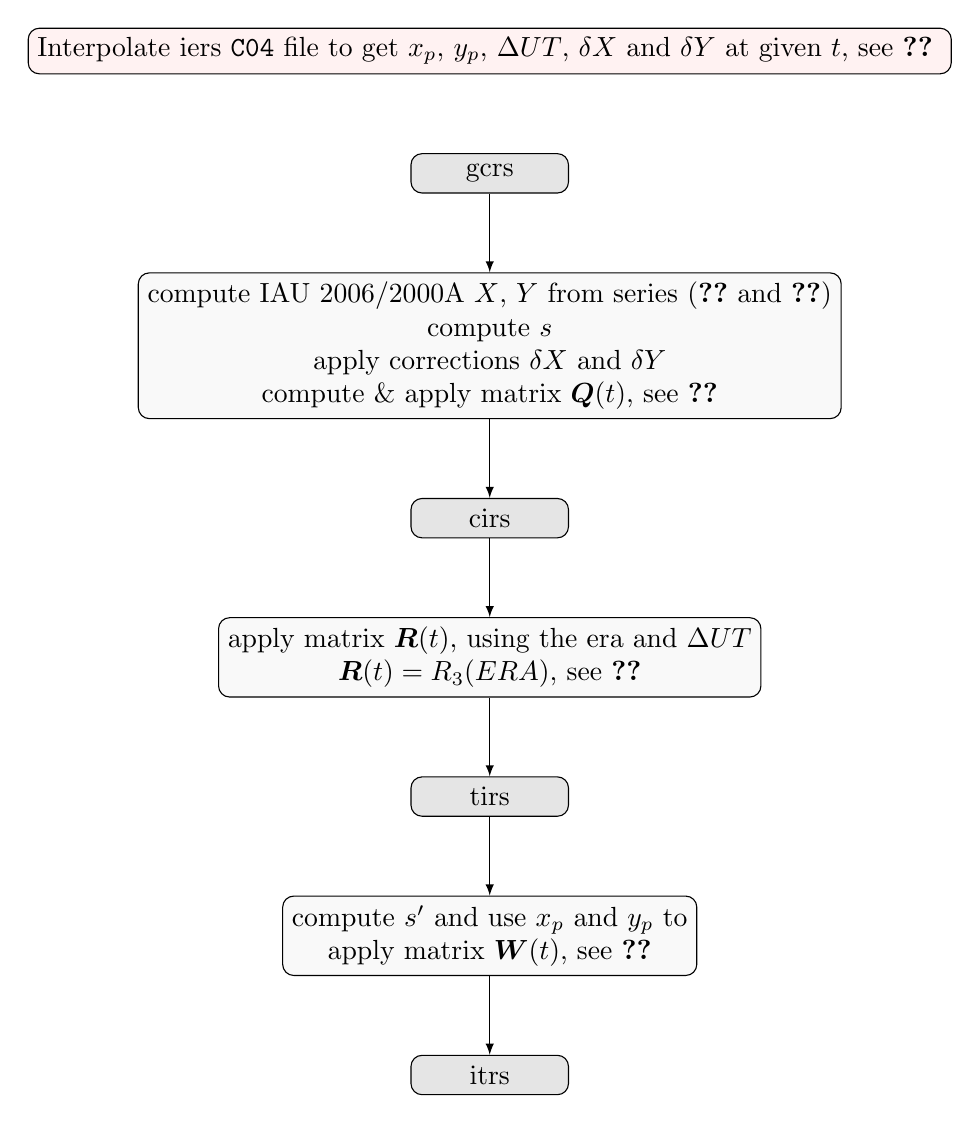
\begin{tikzpicture}[
  every node/.style = {
    draw=black, 
    rounded corners, 
    fill=gray!20,
    minimum width=2cm,
    minimum height=0.5cm,
    align=center},
    every path/.style = {draw, -latex}
  ]
  
  \node[fill=red!5] (c04) [] {
    Interpolate \gls{iers} \texttt{C04} file to get $x_p$, $y_p$, $\Delta UT$, 
    $\delta X$ and $\delta Y$ at given $t$, see \ref{fig:handling-eop}
  };

  \node (gcrs) [below=of c04] {\acrfull{gcrs}};
  
  \node[fill=gray!5] (gcrs2cirs) [below =of gcrs] {
    compute IAU 2006/2000A $X$, $Y$ from series (\ref{eq:tn36516a} and \ref{eq:tn36516b})\\ 
    compute $s$ \\
    apply corrections $\delta X$ and $\delta Y$\\
    compute \& apply matrix $\bm{Q}(t)$, see \ref{par:celestial-motion-matrix}
  };

  \node (cirs) [below =of gcrs2cirs] {\acrfull{cirs}};

  \node[fill=gray!5] (cirs2tirs) [below =of cirs] {
    apply matrix $\bm{R}(t)$, using the \gls{era} and $\Delta UT$\\
    $\bm{R}(t) = R_3 (ERA) $, see \ref{par:earth-rotation-matrix}
  };
  
  \node (tirs) [below =of cirs2tirs] {\acrfull{tirs}};

  \node[fill=gray!5] (tirs2itrs) [below =of tirs] {
    compute $s'$ and use $x_p$ and $y_p$ to\\
    apply matrix $\bm{W}(t)$, see \ref{par:polar-motion-matrix}
  };
  
  \node (itrs) [below =of tirs2itrs] {\acrfull{itrs}};

  \draw (gcrs) -- (gcrs2cirs);
  \draw (gcrs2cirs) -- (cirs);
  \draw (cirs) -- (cirs2tirs);
  \draw (cirs2tirs) -- (tirs);
  \draw (tirs) -- (tirs2itrs);
  \draw (tirs2itrs) -- (itrs);

\end{tikzpicture}

  \caption{Schematic representation of the ``\gls{cio}-based'' procedure to 
    transform between the \gls{gcrs} and \gls{itrs}.}
  \label{fig:itrf-to-icrf}
\end{figure}

\paragraph{Polar Motion Matrix $W(t)$}\label{par:polar-motion-matrix}
The rotation of the Earth is represented by the diurnal rotation around a
reference axis, called the \gls{cip}. The \gls{cip} does not coincide with 
the axis of figure of the Earth, but slowly moves (in a terrestrial reference 
frame) (\cite{Urban2013}). This motion of the terrestrial reference frame 
with respect to the \gls{cip} is known as \emph{polar motion}. Note that the 
\gls{cip} is not the instantaneous axis of rotation but the axis around which the 
diurnal rotation of earth is applied (in the celestial to terrestrial 
transformation). Polar motion is typically determined from \gls{vlbi} 
observation, as except from the principal periods of 365 days (annual wobble) 
and 428 days (Chandler wobble), it is also affected by unpredictable geophysical 
forces.

According to IAU 2006 Resolution B2, the system at date $t$ as realized 
from the \gls{itrs} by applying the transformation $\bm{W}(t)$ is the 
\gls{tirs}. It uses the \gls{cip} as its $z$-axis and the \gls{tio} as 
its $x$-axis (\cite{iers2010}). This matrix gives the position of the 
terrestrial reference frame with respect to the \gls{tio}.

The $\bm{W}$ matrix can be expressed as (\cite{iers2010}):
\begin{equation}
    \bm{W}(t) = \bm{R}_z(-s') \cdot \bm{R}_y(x_p) \cdot \bm{R}(y_p)
    \label{eq:iers1053}
\end{equation}
where $s'$ is the ``\gls{tio} locator'' and $x_p$, $y_p$ are the 
``polar coordinates'' of the \gls{cip} in the \gls{itrs}. The latter values, 
if not estimated, should be the ones published by the \gls{iers}, corrected for 
the effect of ocean tides and forced terms (aka ``libration''), with periods 
less than two days in space (\cite{iers2010}), see \autoref{ssec:eop-interpolation}.

The \gls{tio} locator $s'$, positioning the \gls{tio} on the equator of the \gls{cip}, 
is necessary to provide an exact realization of the ``instantaneous prime meridian'', 
designated by ``\gls{tio} meridian'' (\cite{iers2010}). $s'$ is obtained from 
polar motion observations by numerical integration, and so is in essence 
unpredictable. However, it is dominated by a secular drift of about 
\SI{47}{\micro\larcsecond\per\century}. The latter is used to actually compute 
$s'$ in \autoref{eq:iers1053}.
%\footnote{In accordance to the \gls{sofa} (\cite{SOFA20210125}) supplied \texttt{iauSp00} function} 
using the function:
\begin{equation}
  s' = \SI{-47}{\micro\larcsecond} \cdot t
  \label{eq:iers10513}
\end{equation}
obtained from C04 data (\cite{Lambert2002}).

%The $\bm{W}(t)$ matrix is computed using a variant of the \gls{sofa} (\cite{SOFA20210125}) 
%supplied \texttt{iauPom00} function.

\paragraph{Earth Rotation Matrix $R(t)$}\label{par:earth-rotation-matrix}
The rotation of the Earth around the axis of the \gls{cip} (i.e. relating 
\gls{tirs} and \gls{cirs}), can be expressed as (\cite{iers2010}):
\begin{equation}
  \bm{R}(t) = \bm{R}_z (-ERA)
  \label{eq:iers1055}
\end{equation}
where $ERA$ is the \gls{era} between the \gls{cio} and the \gls{tio} 
at date $t$ on the equator of the \gls{cip}, which is the rigorous definition 
of the sidereal rotation of the Earth. Working with respect to the \gls{cio} 
(rather than the equinox) sweeps away sidereal time's complexities and opportunities 
for error. The Earth rotation angle, the \gls{cio} based counterpart of \gls{gst},
is simply a conventional linear transformation of \gls{ut1} (\cite{sofa_18141_eacb}):
\begin{equation}
  \label{eq:iers10515}
  \begin{split}
    ERA(T_u) = 2 \pi & ( \text{UT1 Julian day fraction } \\
                     & + 0.7790572732640 + 0.00273781191135448 \cdot T_u )
    \end{split}
\end{equation}
where $T_u = \left( \text{Julian UT1 date } - 2451545.0 \right)$ and 
$UT1=UTC+(UT1-UTC)$. 

Similarly to polar motion, additional components should 
be added to the values published by \gls{iers} for $\Delta UT$ to account for 
the effects of ocean tides and libration, see \autoref{ssec:eop-interpolation}. 

\paragraph{Celestial Motion Matrix $Q(t)$}\label{par:celestial-motion-matrix}
The \gls{cio} based transformation matrix arising from the motion of the \gls{cip} 
in the \gls{gcrs} (i.e. relating \gls{cirs} and \gls{gcrs}), can be expressed as
(\cite{iers2010}):
\begin{equation}
  \bm{Q}(t) = \bm{R}_z (-E) \cdot 
              \bm{R}_y (-d) \cdot 
              \bm{R}_z (E) \cdot 
              \bm{R}_Z (s)
  \label{eq:iers1056}
\end{equation}
where $s$ is the ``\gls{cio} locator'' and $E$ and $d$ being such that the 
coordinates of the \gls{cip} in the \gls{gcrs} are:
\begin{equation}
  \begin{aligned}
    X & = \sin{d} \cos{E} \\
    Y & = \sin{d} \sin{E} \\
    Z & = \cos{d}
  \end{aligned}
\end{equation}
\autoref{eq:iers1056} can be given in an equivalent form directly involving $X$ and 
$Y$ as (\cite{iers2010}):
\begin{equation}
  \bm{Q}(t) = \begin{pmatrix}
    1-\alpha X^2 & -\alpha XY & X \\
    -\alpha XY & 1-\alpha Y^2 & Y \\
    -X & -Y & 1-\alpha (X^2 + Y^2) \end{pmatrix}
    \cdot \bm{R}_Z (s)
    \label{eq:iers10510}
\end{equation}
with $\alpha = 1/(1+\cos{d})$ , which can also be written, with an accuracy of 
\SI{1}{\micro\larcsecond} as $\alpha = 1/2 + 1/8(X^2 + Y^2)$.

$X$ and $Y$ coordinates can be given by developments as function of time in the 
\si{\micro\larcsecond} level, based on the IAU 2006 precession and IAU 2000A
nutation (\cite{Capitaine2006a}).
%\footnote{Implemented in the \gls{sofa} (\cite{SOFA20210125}) supplied \texttt{iauXy06} function.}
The IAU 2006/2000A developments are as follows (\cite{iers2010}):
\begin{equation}
  \label{eq:tn36516a}
  \begin{aligned}
  X &= \SI{-0.01661700}{\arcsecond} + \SI{2004.19189800}{\arcsecond} t - \SI{0.429782900}{\arcsecond} t^2 \\
  &- \SI{0.1986183400}{\arcsecond}t^3 + \SI{0.00000757800}{\arcsecond} t^4 + \SI{0.000005928500}{\arcsecond} t^5 \\
  &+ \sum_{i} \left[ (a_{s,0})_i \sin \theta + (a_{c,0})_i \cos \theta \right] \\ 
  &+ \sum_{i} \left[ (a_{s,1})_i t \sin \theta + (a_{c,1})_i t \cos \theta \right] \\ 
  &+ \sum_{i} \left[ (a_{s,2})_i t^2 \sin \theta + (a_{c,2})_i t^2 \cos \theta \right] \\ 
  &+ \cdots \\
  \end{aligned}
\end{equation}
and
\begin{equation}
  \label{eq:tn36516b}
  \begin{aligned}
  Y &= -\SI{0.00695100}{\arcsecond} - \SI{0.02589600}{\arcsecond} t - \SI{22.407274700}{\arcsecond} t^2 \\
  &+ \SI{0.0019005900}{\arcsecond} t^3 + \SI{0.00111252600}{\arcsecond} t^4 + \SI{0.000000135800}{\arcsecond} t^5 \\
  &+ \sum_{i} \left[ (b_{s,0})_i \sin \theta     + (b_{c,0})_i \cos \theta \right] \\ 
  &+ \sum_{i} \left[ (b_{s,1})_i t \sin \theta   + (b_{c,1})_i t \cos \theta \right] \\ 
  &+ \sum_{i} \left[ (b_{s,2})_i t^2 \sin \theta + (b_{c,2})_i t^2 \cos \theta \right] \\ 
  &+ \cdots \\
  \end{aligned}
\end{equation}

where $\theta$ is a function of the fundamental lunisolar and planetary arguments.
Further information and computation formulas for the fundamental arguments, 
can be found in \cite{iers2010}, e.g. Chapter 5.7. Complete 
list of coefficients for \autoref{eq:tn36516a} and \autoref{eq:tn36516b} is provided 
by \gls{iers}. 

\gls{vlbi} observations have shown that there are deficiencies in the 
IAU 2006/2000A precession-nutation model of the order of \SI{0.2}{\milli\larcsecond}, 
mainly due to the fact that the free core nutation (\gls{fcn}) is not part of 
the model, \gls{iers} publish observed estimates of the corrections to the 
IAU precession-nutation model. The observed differences with respect to the 
conventional celestial pole position defined by the models are monitored and 
reported by the \gls{iers}as ``celestial pole offsets''. Such time-dependent 
offsets from the direction of the pole of the \gls{gcrs} must be provided as 
corrections $\delta X$ and $\delta Y$ to the $X$ and $Y$ coordinates (\cite{iers2010}).
Using these offsets, the corrected celestial position of the \gls{cip} is 
given by (\cite{iers2010}):
\begin{equation}
  \begin{aligned}
    X = X_{\text{IAU 2006/2000}} + \delta X \\
    Y = Y_{\text{IAU 2006/2000}} + \delta Y
  \end{aligned}
\end{equation}
thus enabling to re-write \autoref{eq:iers10510} as:
\begin{equation}
  \bm{\tilde{Q}}(t) = \begin{pmatrix}
    1 & 0 & \delta X \\
    0 & 1 & \delta Y \\
    -\delta X & -\delta Y & 1
    \end{pmatrix}
    \cdot \bm{Q}_{IAU}
    \label{eq:iers10527}
\end{equation}
where $\bm{Q}_{IAU}$ represents the $\bm{Q}(t)$ matrix based on the IAU 2006/2000 
precession-nutation model.

The ``\gls{cio} locator'' $s$, providing the position of the \gls{cio} in the 
\gls{gcrs} can also be computed using a development described in \cite{Capitaine2003}.
%\footnote{\gls{sofa} (\cite{SOFA20210125}) supplies an implementation of the formula named \texttt{iauS06} function}.

      \subsection{Earth Orientation Parameters Information And Interpolation}\label{ssec:eop-interpolation}

\Gls{eop} information for formulating the Celestial-to-Terrestrial transformation 
matrix, is extracted from the \gls{iers} \texttt{C04} files (\cite{Bizouard2019}).
These files contain tabulated \gls{eop} values ($x_p$, $y_p$, $\delta UT1$, $LOD$ and 
the celestial pole offsets $\delta X$ and $\delta Y$) at 0\textsuperscript{h} \gls{utc}. 
$LOD$ and celestial pole offsets contain the most dramatic variation over time, while 
the pole coordinates and time offset parameters exhibit much smoother variations.

In general, the tabulated pole coordinates, $\delta UT1$ and $LOD$ values must first 
be interpolated to the appropriate time and then corrected for ocean tide and 
libration effects. The ocean tide corrections, include diurnal and semi-diurnal 
variations caused by ocean tides for polar motion, $\delta UT1$ and $LOD$. Libration effects, 
include diurnal and semi-diurnal nutations that originate from the direct effect 
of the external (mainly luni-solar) torque on the non-axisymmetric part of the Earth 
(\cite{iers2010} and references therein) and like ocean tide corrections, have an effect on 
pole coordinates as well as $\delta UT1$ and $LOD$. The variations of these effects 
have to be accounted for when using the published values for \gls{eop} parameters.

Especially for $\delta UT1$ and $LOD$, according to \cite{Bradley2016}, 
prior to their interpolation, ``the tabulated values should be smoothed through regularization 
to enhance the interpolation accuracy''. Regularization is the removal of zonal tidal 
variations with frequencies ranging from 5 days to 18.6 years. This ``regularization'' is 
implemented in the \gls{eop} interpolation process.

For the current Thesis, the process described above was designed and implemented, for 
extracting \gls{eop} information from \texttt{C04} files, storing values in efficiently designed 
data structures, and performing the interpolation along with the corrections described above.
A schematic representation is given in \autoref{fig:handling-eop}. As shown in 
\autoref{fig:eop-interpolation-results}, including the ocean tide and libration 
effects, allows for the introduction of diurnal and semi-diurnal signals.

\begin{figure}
  \centering
  \includegraphics[height=.4\textheight,keepaspectratio]{eop_interpolation}
  \caption{Interpolation of \gls{eop} parameters $x_p$, $y_p$, $\delta UT1$ and $LOD$ 
      performed by the software developed, following \ref{fig:handling-eop}. Red crosses 
      represent the input, reference \gls{eop} values.}
  \label{fig:eop-interpolation-results}
\end{figure}

For the polar motion \gls{eop}, $x_p$ and $y_p$,
\begin{equation}
    \begin{pmatrix} x_p & y_p \end{pmatrix} = 
    \begin{pmatrix} x & y \end{pmatrix}_{IERS} + 
    \begin{pmatrix} \Delta x & \Delta y \end{pmatrix}_{ocean\text{ }tides} + 
    \begin{pmatrix} \Delta x & \Delta y \end{pmatrix}_{libration} 
\end{equation}
where $\begin{pmatrix} \Delta x & \Delta y \end{pmatrix}_{ocean\text{ }tides}$ 
and $\begin{pmatrix} \Delta x & \Delta y \end{pmatrix}_{libration}$ are computed as 
outlined in \cite{iers2010}; the former is achieved by a software routine designed 
on the basis of the \texttt{ORTHO\_EOP}\footnote{Available from the \gls{iers} \href{https://iers-conventions.obspm.fr/}{Conventions Centre} at \url{https://iers-conventions.obspm.fr/content/chapter8/software/ORTHO_EOP.F}, provided by R. Eanes.\label{fn:ortho-eop-f}} 
to compute the diurnal and semidiurnal variations in the Earth orientation, while the latter 
is based on \texttt{PMSDNUT2}\footnote{Available from the \gls{iers} \href{https://iers-conventions.obspm.fr/}{Conventions Centre} at \url{https://iers-conventions.obspm.fr/content/chapter5/software/PMSDNUT2.F}, provided by A. Brzezinski. \label{fn:pmsdnut2-f}}
to compute the diurnal lunisolar effect on polar motion, see \autoref{fig:handling-eop}.

Similarly, for the $\delta UT1$ and $LOD$ values, 
\begin{equation}
    \begin{pmatrix} \delta UT1 & LOD \end{pmatrix} = 
    \begin{pmatrix} x & y \end{pmatrix}_{IERS} + 
    \begin{pmatrix} \delta UT1 & LOD  \end{pmatrix}_{ocean\text{ }tides} + 
    \begin{pmatrix} \delta UT1 & LOD  \end{pmatrix}_{libration} 
\end{equation}
where again $\begin{pmatrix} \delta UT1 & LOD  \end{pmatrix}_{ocean\text{ }tides}$ 
are computed using the same procedure as above, while $\begin{pmatrix} \delta UT1 & LOD  \end{pmatrix}_{libration}$ 
are computed using a software routine designed on the basis of the \gls{iers}-published 
\texttt{UTLIBR}\footnote{Available from the \gls{iers} \href{https://iers-conventions.obspm.fr/}{Conventions Centre} at \url{https://iers-conventions.obspm.fr/content/chapter5/software/UTLIBR.F}, provided by A. Brzezinski.\label{fn:utlibr-f}} 
to account for the subdiurnal librations.

The linear interpolation is based on a Lagrangian interpolation scheme, generic enough to 
perform interpolation of any order (given enough data). For \gls{pod}, a 5-order 
interpolation procedure is performed, based on results from \cite{Bradley2016}. 

Optionally, users can perform the ``regularization'' of $\delta UT1$ and $LOD$ values. 
In this case, prior to the interpolation the tabulated values are smoothed through 
regularization to enhance the interpolation accuracy. After regularization and 
interpolation, the zonal tide value should be added back at the time of interpolation.
At this point, the ocean tide corrections should be computed and added to the 
interpolated values. The zonal tide effects are based on models recommended by 
the \gls{iers} Conventions and the distributed \texttt{RG\_ZONT2}
%\footnote{Available from the \gls{iers} \href{https://iers-conventions.obspm.fr/}{Conventions Centre} at 
%\url{https://iers-conventions.obspm.fr/content/chapter5/software/PMSDNUT2.F}, provided by A. Brzezinski. \label{fn:rg-zont2-f}}.

%\begin{table}
%\centering
%\begin{tabular}{|p{3cm}|p{3cm}|p{2.5cm}|p{5cm}|}
%    \hline
%    \textbf{Function/Data Structure} & \textbf{Header File} & \textbf{Repository/ Library} & \textbf{Comment} \\
%    \hline
%    \texttt{EopLookUpTable} & \texttt{eop.hpp} & \texttt{doris} & 
%    Contains all relevant declerations, data structures and algorithms to handle 
%    \gls{eop} information. \\
%
%    \hline
%    \texttt{parse\_iers\_C04} & \texttt{eop.hpp} & \texttt{doris} & \\
%
%    \hline
%    \texttt{ortho\_eop} & \texttt{iers2010.hpp} & \texttt{iers2010} &
%    compute the diurnal and semidiurnal variations in \gls{eop} ($x$,$y$, $UT1$) from
%    ocean tides; translated from \texttt{ORTHO\_EOP.F} \footref{fn:ortho-eop-f} \\
%
%    \hline
%    \texttt{pmsdnut2} & \texttt{iers2010.hpp} & \texttt{iers2010} &
%    evaluate the model of polar motion for a nonrigid Earth due to tidal gravitation; 
%    translated from \texttt{PMSDNUT2.F} \footref{fn:pmsdnut2-f} \\ 
%
%    \hline
%    \texttt{utlibr} & \texttt{iers2010.hpp} & \texttt{iers2010} & 
%    compute subdiurnal libration in the axial component of rotation, expressed by 
%    \gls{ut1} and LOD. This effect is due to the influence of tidal gravitation on the
%    departures of the Earth's mass distribution from the rotational
%    symmetry, expressed by the non-zonal components of geopotential. Translated 
%    from \texttt{UTLIBR.F} \footref{fn:utlibr-f} \\
%
%    \hline
%    \texttt{interp\_pole} (and \texttt{interp} namespace) & \texttt{iers2010.hpp} & \texttt{iers2010} & 
%    account for ocean tidal and libration effects in \gls{eop}; translated from \texttt{INTERP.F} \footref{fn:interp-f}\\
%
%    \hline
%\end{tabular}
%\caption{List of functions and data structures relevant to handling \gls{eop} information.}
%\label{table:eop-handling-fds}
%\end{table}


\begin{figure}
\centering
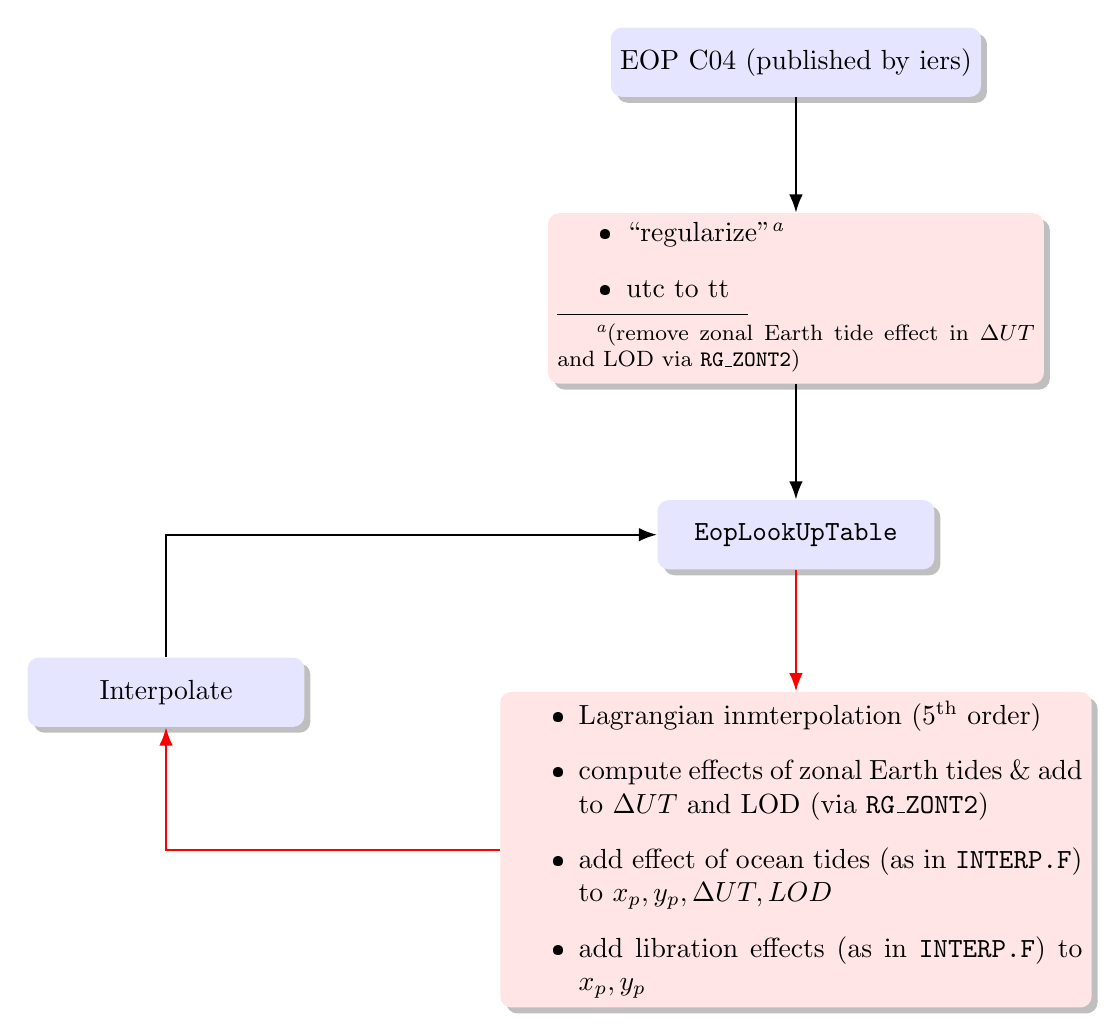
\begin{tikzpicture}
	\node (A) at (0,0) 
		[minimum height=2.5em, minimum width=10em, fill=blue!10,rounded corners, drop shadow] 
		{EOP C04 (published by \gls{iers})};
	
	\node (AtB) at (0,-3) 
		[minimum height=2.5em, minimum width=10em, fill=red!10,rounded corners, drop shadow]
		{\begin{minipage}{.5\textwidth}\begin{itemize}
		\item ``regularize''\footnote{(remove zonal Earth tide effect in $\Delta UT$ and LOD via \texttt{RG\_ZONT2})}
		\item \gls{utc} to \gls{tt}
		\end{itemize}\end{minipage}};
		
	\node (B) at (0,-6.0) 
		[minimum height=2.5em, minimum width=10em, fill=blue!10,rounded corners, drop shadow] 
		{\texttt{EopLookUpTable}};

	\node (BtI) at (0,-10) 
		[minimum height=2.5em, minimum width=10em, fill=red!10,rounded corners, drop shadow]
		{\begin{minipage}{.6\textwidth}\begin{itemize}
		\item Lagrangian inmterpolation (5\textsuperscript{th} order)
		\item compute effects of zonal Earth tides \& add to $\Delta UT$ and LOD (via \texttt{RG\_ZONT2})
		\item add effect of ocean tides (as in \texttt{INTERP.F}) to $x_p, y_p, \Delta UT, LOD$
		\item add libration effects (as in \texttt{INTERP.F}) to $x_p, y_p$
		\end{itemize}\end{minipage}};
	
	\node (I) at (-8,-8)
		[minimum height=2.5em, minimum width=10em, fill=blue!10,rounded corners, drop shadow]
		{Interpolate};

	\draw[-Latex,thick] (A.south) -- (AtB.north);
	\draw[-Latex,thick] (AtB.south) -- (B.north);
	\draw[-Latex,thick] (I.north) |- (B.west);
	\draw[-Latex,red,thick] (B.south) -| (BtI.north);
	\draw[-Latex,red,thick] (BtI.west) -| (I.south);
	%\draw[->] (A)--(B) node[midway]{Remove effects of zonal Earth tides on $\Delta$UT and LOD (\texttt{rg\_zont2})}; 
\end{tikzpicture}

\caption{Extracting \gls{eop} information from \gls{iers} \texttt{C04} data files.}
\label{fig:handling-eop}
\end{figure}

    
    \section{Time Systems and Scales}\label{ssec:time-systems-and-scales}
      \subsection{A Short Introduction to Time Scales}\label{ssec:time-scales}

Historically, solar time was the basis of time keeping, based on the diurnal rotation
of the Earth. However, with the  discovery of the variability of the 
rate of rotation of the Earth and later on the development of atomic clocks, 
ans the SI second different time systems and scales have been introduced to match the 
ever growing precision demands.

\begin{table}[h!]
    \centering
    \begin{tabular}{p{7cm}p{5cm}p{1cm}}
        %\hline
        \textbf{Time Scale} & \textbf{Usage\footnote{As in \cite{sofa2021ts}.}} & \textbf{Type} \\
        \hline
        \gls{tai} & the official timekeeping standard & Atomic \\
        %\arrayrulecolor{gray}\hline
        \gls{utc} & the basis of civil time & Atomic/Solar hybrid\\
        %\arrayrulecolor{gray}\hline
        \gls{ut1} & based on Earth rotation & Solar \\
        %\arrayrulecolor{gray}\hline
        \gls{tt}  & used for solar system ephemeris look-up & Dynamical\\
        %\arrayrulecolor{gray}\hline
        \gls{tcg} & used for calculations centered on the Earth in space  & Dynamical\\
        %\arrayrulecolor{gray}\hline
        \gls{tcb} & used for calculations beyond Earth orbit  & Dynamical\\
        %\arrayrulecolor{gray}\hline
        \gls{tdb} & a scaled form of \gls{tcb} that keeps in step with \gls{tt} on the average  & Dynamical\\
        \hline
    \end{tabular}
    \caption{Fundamental time scales used in Geodesy and Astronomy.}
    \label{table:time-scales}
  \end{table}

\paragraph{\gls{tai}}\label{par:tai}
The unit of \gls{tai} is the SI second, defined as ``the duration of 9,192,631,770 periods 
of the radiation corresponding to the transition between the two hyperfine levels of the ground state 
of the caesium 133 atom''. \gls{tai} is a laboratory time scale, independent of 
astronomical phenomena apart from having been synchronized to solar time when first 
introduced. It is realized via a weighted average of a number of high-precision atomic 
clocks held around the world. It is close to proper time for an observer on the
geoid, and is an appropriate choice for terrestrial applications (\cite{sofa2021ts}).

\paragraph{\gls{utc}}\label{par:utc}
\gls{utc} is a compromise between the demands of precise timekeeping and the desire to maintain
the current relationship between civil time and daylight. Untill 1972, rate changes were 
introduced to keep \gls{utc} roughly in step with \gls{ut1}; since then, adjustments have been 
made by occasionally inserting a whole second, called a \emph{leap second}, a procedure 
that can be thought of as stopping the \gls{utc} clock for a second to let the Earth catch 
up (\cite{sofa2021ts}). Leap seconds are introduced as necessary to keep \gls{ut1}-\gls{utc} in the
range $\pm\SI{0.9}{\second}$. The difference between \gls{ut1} and \gls{utc} is usually 
designated as $\Delta AT$.

\paragraph{\gls{ut1}}\label{par:ut1}
\gls{ut1} is the modern equivalent of mean solar time. In a physical sense, it is an 
angle rather than actual time, and is defined through its relationship with Earth 
rotation angle. Because of the variability of Earth's rotation, \gls{ut1} second is not 
precisely matched to the SI second. The difference between \gls{ut1} and \gls{tt} 
is normally designated as $\Delta T$, and can be written out as
\begin{equation}
    \Delta T = TT - UT1 = \SI{32.184}{\second} + \Delta AT - \Delta UT1
\end{equation}

\paragraph{The Dynamical Time Scales \gls{tcg}, \gls{tcb} \& \gls{tdb}}
\label{par:dynamical-time-scales}
The coordinate time scales \gls{tcg}, \gls{tcb} and \gls{tdb} are the independent
variable in General Relativity based theories which describe the motions of bodies in 
the vicinity of the Earth (\gls{tcg}) and in the solar system (\gls{tcb}, \gls{tdb}).
\gls{tt} and \gls{tdb} are close to each other (less than \SI{2}{\milli\second}) and 
run at the same rate as \gls{tai} (exactly in the case of \gls{tt}). \gls{tcg}
and \gls{tcb}, used in theoretical work, run at different rates and so have long 
term drifts relative to \gls{tai} (\cite{sofa2021ts}). \gls{tcg} and \gls{tcb} are 
the time coordinates of two \gls{iau} spacetime metrics called, respectively, the
geocentric and barycentric celestial reference systems (\gls{gcrs} and \gls{bcrs}).
\gls{tcg}, is appropriate for theoretical studies of geocentric ephemerides.
Its relationship with \gls{tt} is this conventional linear transformation:
\begin{equation}
    TCG = TT + L_G \times (JD_{TT} - TT_{0})
\end{equation}
where $TT_0 = 2443144.5003725$ (i.e. TT at 1977 January 1.0 TAI) and 
$LG = 6.969290134 \times 10-10$. The rate change $LG$ means that \gls{tcg} gains about
\SI{2.2}{\second} per century with respect to \gls{tt} or \gls{tai}; this represents 
the combined effect on the terrestrial clock of the gravitational potential from the 
Earth and the observatory's diurnal speed (\cite{sofa2021ts}).


\paragraph{\gls{tt}}\label{par:tt}
\gls{tt}, is the theoretical time scale for clocks at sea-level (on the geoid): for 
practical purposes it is tied to \gls{tai} through
\begin{equation}
    TT = TAI + \SI{32.184}{\second}
\end{equation}


Note that UTC has to be expressed as hours, minutes and seconds (or at least in seconds in a
given day) if leap seconds are to be taken into account in the correct manner. In particular, it
is inappropriate to express UTC as a Julian Date, because there will be an ambiguity during a
leap second—so that for example 1994 June 30 23h 59m 60s.0 and 1994 July 1 00h 00m 00s.0 would
both come out as MJD 49534.00000—and because subtracting two such JDs would not yield the
correct interval in cases that contain leap seconds.

      \subsection{Implementing Time Scales}\label{ssec:time-scales-implementation}

Designing and implementing software for handling dates, time scales and related transformations 
is a rather challenging task. The complexity is evident, considering:
\begin{itemize}
    \item The long list of different time-scales involved in Satellite Geodesy and 
        Astronomy (see \ref{ssec:time-scales})
    \item The different representation conventions (e.g. \gls{jd}, \gls{mjd}, year/month/day and hour/minute/seconds)
    \item The accuracy required when transforming between different time scales 
    \item The heavy usage of dates and time in a \gls{pod} process (i.e. efficiency)
\end{itemize}

All of the above must be taken into account in software design, making the ``datetime'' 
problem a field of continuous investigation. Despite the fact that there are a few datetime libraries, 
(some languages have even relevant implementations in their standard libraries), none 
complies with the accuracy and complexity involved in Satellite Geodesy. The exception 
is the official \gls{iau} implementation of Fundamental Astronomy, i.e. the \gls{sofa} 
library (\cite{sofa2021}). However, \gls{sofa} is implemented in the FORTRAN (and C) 
programming languages and has to reserve a level of ``backwards compatibility'', thus 
its design paradigm is rather outdated (e.g. no Object Oriented Design). Additionally, 
the package provides core functionality, hence one should implement various utility functions 
(e.g. parsers) to interact with this functions.

For all the above, a decision was taken to design and implement a new software library, 
from scratch, to address the ``datetime'' problem. The design follows recent developments 
and paradigms in Software Engineering, such as Template Metaprogramming 
(\cite{Vandevoorde2017}). The library is open and free for any interested user.

A ``datetime'' or \emph{epoch} within the library is represented as an \gls{mjd}, 
where the integral and fractional part of day are stored separately, to preserve 
precision. In the special case of \gls{utc} dates, the epoch can be stored in the 
Year Month Date plus Hours Minutes Seconds (YMD/HMS) format. Depending on the user/application 
needs, the fractional part of the day can be stored as either a floating point numeric 
value, or the accumulated number of \si{\second}, \si{\milli\second}, \si{\micro\second} or 
\si{\nano\second}, since the beginning of the day. Both implementations are supported by 
individual ``classes''; the latter is achieved via heavy template usage. 

While storing the fractional part of day as a floating point number is intuitive and 
straightforward, it suffers from roundoff errors. This is avoided in the case where 
the fraction of day is stored as an integer numeric value (i.e. accumulated second 
submultiple); however, in this case, precision is limited by the chosen submultiple 
and non-integer division will also introduce truncation. It is up to the user to 
choose the suitable representation to meet application demands.

The components of the library have been extensively tested using the \gls{sofa} results 
as reference, as well as the relevant (limited) standard library functions. The 
software is developed as a stand-alone library, complying with the latest C++ standards 
(C++17 \& C++20) and include $\approx$5000 lines of source code (including test suits).

%\fi

\chapter{Orbit Integration}\label{ch:orbit-integration}
%\iffalse
  \section{Introduction}\label{sec:integration-introduction}

The equations of motion governing the orbital path followed by an Earth orbiting 
satellite, constitute a system of \glspl{ode}. To ``propagate'' the orbit, we need 
to solve this system, using a reference trajectory at a given instant $t=t_0$ as 
\emph{initial conditions}. The high accuracy that is nowadays required for \gls{pod} 
applications, can only be achieved via numerical methods (\cite{Montenbruck2000}).

A variety of methods have been successfully applied to the problem of orbit 
propagation, each with its own drawbacks, limitations and advantages (see e.g. 
\cite{Somodi2011} and \cite{Papanikolaou2016}\info{Added references here})
. Thus, in 
general, it is not possible to simply select one method as best suited for the 
prediction of satellite motion.

In this Thesis, we investigate two kind of integration techniques, namely:
\begin{description}
    \item[Runge—Kutta] methods, that have the advantage of being well established 
      and easy to implement, and
    \item[multistep] methods, that a high efficiency and accuracy at a cost of 
      increased implementation complexity
\end{description}
Both of these techniques, are further subdivided into more specialized algorithms, 
depending on problem constraints, choice of parameters and algorithmic approach. 
Typically, application needs indicate the appropriate methodology.

It should be noted that the equations of motions considered, constitute a system 
of \glspl{ode} of seconds degree. Even though methods for direct integration of 
such equations exist, they will not be considered here, since such methods assume 
that forces acting on a satellite do not depend on its velocity (an assumption not 
fulfilled in the \gls{pod} case, see e.g. \autoref{sssec:atmospheric-drag}).
For a more detailed and general discussion on numerical methods for \glspl{ode}, 
see \cite{Hairer2009I} and \cite{Hairer2010II}.

A first order system of \glspl{ode} can always be obtained from a respective second 
order, by combining the position $\bm{r}$ and velocity $\bm{\dot{r}}$ vectors into 
the 6-dimensional \emph{state vector} $\bm{y}$
\begin{equation}
    \bm{y} = \begin{pmatrix}\bm{r}\\ \bm{\dot{r}} \end{pmatrix}
\end{equation}
with 
\begin{equation}
    \bm{\dot{y}} = \bm{f}(t,\bm{y}) = \begin{pmatrix}\bm{\dot{r}} \\ \bm{a}(t, \bm{r}, \bm{\dot{r}}) \end{pmatrix}
\end{equation}
so that the original system
\begin{equation}
    \bm{\ddot{r}} = \bm{a}(t, \bm{r}, \bm{\dot{r}})
\end{equation}
can be written in the general form
\begin{equation}\label{eq:genode0}
    \bm{\dot{y}} = \bm{f}(t,\bm{y}), \text{ with } \bm{y}, \bm{\dot{y}}, \bm{f} \in \Re
\end{equation}

  \section{Runge-Kutta Methods}\label{sec:runge-kutta}

In the \emph{Runge-Kutta} methods, a weighted average of the slopes ($\bm{f}$) of 
the solution computed at nearby points is used to determine the solution at 
$t = t_{n+1}$ from that at $t = t_n$. Typically, Runge-Kutta methods are further 
divided in \emph{explicit} and \emph{implicit} methods; the latter are more complicated 
but allow for higher order and improved stablity (see \cite{Griffiths2010}).

The general $s$-stage Runge-Kutta methods, may be written in the form
\begin{equation}\label{eq:grif95}
    x_{n+1} = x_n + h \sum_{i=1}^{s} b_i k_i 
\end{equation}
where the $k_i$ terms can be computed from the function $f$
\begin{equation}\label{eq:grif96}
    k_i = f \left( t_n + c_i h , x_n + h \sum_{j=1}^{s} a_{i,j} k_j \right) \text{ with } i = 1,2,\dots s
\end{equation}
Typically, we impose the condition
\begin{equation}
    c_i = \sum_{j=1}^{s} a_{i,j}
\end{equation}
Thus, given a value of $s$, the method depends on $s^2 + s$ parameters $a_{i,j}$ and $b_j$.
These can be conveniently displayed in a tableau known as the \emph{Butcher array} 
(see e.g. \cite{Butcher2016}).

\noindent\begin{minipage}[t]{0.5\textwidth}%
    \centering
    \label{table:butcher-array-implicit}
    \begin{tabular}{c|cccc}
        $c_1$  & $a_{1,1}$ & $a_{1,2}$ & \dots & $a_{1,s}$ \\
        $c_2$  & $a_{2,1}$ & $a_{2,2}$ & \dots & $a_{2,s}$ \\
        \vdots & \vdots    & \vdots    &       & \vdots \\ 
        $c_s$  & $a_{s,1}$ & $a_{s,2}$ & \dots & $a_{s,s}$ \\
        \hline
               & $b_1$     & $b_2$     & \dots & $b_s$ \\
    \end{tabular}
    \captionsetup{width=0.8\linewidth}
    \captionof{table}{The Butcher array for a full (implicit) RK method}
\end{minipage}%
\begin{minipage}[t]{0.5\textwidth}%
    \centering
    \label{table:butcher-array-explicit}
    \begin{tabular}{c|ccccc}
        $0$    & $0$       & $0$       & \dots  & $0$         & $0$ \\
        $c_2$  & $a_{2,1}$ & $0$       & \dots  & $0$         & $0$ \\
        $c_3$  & $a_{3,1}$ & $a_{3,2}$ & \dots  & $0$         & $0$ \\
        \vdots & \vdots    & \vdots    & $\ddots$ & $0$         & $0$ \\ 
        $c_s$  & $a_{s,1}$ & $a_{s,2}$ & \dots  & $a_{s,s-1}$ & $0$ \\
        \hline
               & $b_1$     & $b_2$     & \dots & $b_{s-1}$    & $b_s$ \\
    \end{tabular}
    \captionsetup{width=0.8\linewidth}
    \captionof{table}{The Butcher array for an explicit RK method. Zeros are often omitted.}
\end{minipage}%

\autoref{eq:grif96} constitutes a nonlinear equation system of size $s$, that can 
be used to determine $k_i$; once found, they can be substituted into \autoref{eq:grif95} 
to determine $x_{n+1}$. Thus, a general Runge-Kutta method is implicit (\cite{Griffiths2010}).
The form of the Butcher array for an implicit Runge-Kutta method is shown in 
\autoref{table:butcher-array-implicit}. Although early studies were devoted entirely 
to explicit Runge-Kutta methods, interest has now moved to include implicit methods, 
which have become recognized as appropriate for the solution of stiff differential 
equations (\cite{Butcher2016}).

If the coefficients $a_{i,j}$ can be placed in a lower triangular matrix, i.e. 
$a_{i,j} = 0$ for all $j \ge i$, the $k_i$ terms can be computed directly (from 
\autoref{eq:grif96}) without the need to solve any nonlinear equations. These are 
the methods most often used, and are called explicit. In this case, the general form 
of the associated Butcher array is depicted in \autoref{table:butcher-array-explicit}.

The \emph{Local Truncation Error} of a Runge-Kutta method $T_{n+1}$, is defined 
to be the difference between the exact and the numerical solution at $t=t_{n+1}$
(\cite{Griffiths2010})
\begin{equation}
    T_{n+1} = x(t_{n+1}) - x_{n+1}
\end{equation}
with $x_n = x(t_n)$. If $T_{n+1} = \mathcal{O}(h^{p+1})(p>0)$ the method is 
said to be of \emph{order} $p$. In practice, two related Runge-Kutta methods are 
used, one of order $p$ and another of order $p+1$, to approximate the value of 
the local truncation error via $T_{n+1} = x^{p+1}_{n+1} - x^{p}_{n+1}$, where the 
$T_{n+1}$ estimate is for the lowest order method $p$. To perform the calculation 
in an efficient way, the values of $k$s for the lowest degree method, are chosen 
so that they are a subset of the higher degree method coefficients. Such methods 
of neighboring orders are often called \emph{embedded} Runge-Kutta methods.

While for $s<4$ there are always Runge-Kutta methods where $s=q$, this is not the 
case for methods of stages higher than four. The number of stages necessary for 
a given order is known up to order 8, but there are no precise results for higher 
orders (\cite{Griffiths2010}).

\subsection{Adaptive Step Size}\label{ssec:adaptive-step-size}

The step size $h$ is a crucial parameter in the integrations methods; it dictates 
the number of steps required to integrate over a given interval, and the accuracy 
of the results obtained. Small step sizes (in general) improve accuracy but comes 
with an efficiency cost. To that end, \emph{step size control} can be used, to 
compute a value $h_n$ for step $n$, to obtain the same accuracy with fewer steps 
or better accuracy with the same number of steps. In \emph{adaptive} step size control,
the step size in each step is adapted to local conditions, so as to take short steps 
when the solution varies rapidly and longer steps when there is relatively little 
activity. Obviously, computing such variable step sizes, should be automatic and 
inexpensive. A thorough discussion on implementing sophisticated adaptive step size 
control, fit for computer programs, is given in the classic text \cite{Shampine1975}.

  \section{Multistep Methods}\label{sec:multistep-methods}

% http://www.math.iit.edu/~fass/478578_Chapter_2.pdf

\subsection{Adams Method(s)}\label{ssec:adams-method}

%In the Runge-Kutta method (see \autoref{sec:runge-kutta}), each step in the 
%integration process is completely independent and once used for computation is 
%discarded (for this reason they are often called \emph{single-step} methods). 
%To reduce the number of function calls and thus allow for efficiency, \emph{multi-step} 
%methods have been introduced. These store values of previous steps, and reuse them 
%in the next steps to be taken, so that to generate an approximation for the next 
%step, the already computed $x$ and $\dot{x}$ values computed at the previous $k$ 
%steps are combined.
Each step in the integration process in the \emph{Runge-Kutta} method (see 
\autoref{sec:runge-kutta}) is completely independent and is discarded once 
used for computation (this is why they are often referred to as \emph{single-step} 
methods). To cut down on the number of function calls \emph{multi-step} methods 
have been introduced to allow for efficiency. These store previous step values 
and reuse them in the subsequent steps, so that to generate an approximation 
for the next step, the previously computed $y$ and $\dot{y}$ values computed 
at the previous $k$ steps are combined.

In general, starting with the \gls{ode} $\bm{\dot{y}} = \bm{f}(t,\bm{y})$, and 
integrating both sides for the interval $t_i$ to $t_{i+j}$ the following expression 
is obtained
\begin{equation}\label{eq:mont442}
    \bm{y}(t_{i+1}) = \bm{y}(t_i) + \int_{t_i}^{t_{i+1}} \bm{f}(t,\bm{y}(t)) \,dt
\end{equation}
In multistep methods, the integrand is replaced by a polynomial $p(t)$, that interpolates 
a subset of the already available approximate values $\bm{\eta}_j$ of the solutions 
$\bm{y}(t_j)$, such that
\begin{equation}\label{eq:mont443}
    \bm{f}_j = \bm{f}(t_j, \bm{\eta}_j)
\end{equation}
Hence, if $\bm{\eta}_{i+1}$ is the approximate solution at the next step to be taken, 
\begin{equation}
    \bm{\eta}_{i+1} = \bm{\eta}_i + \int_{t_i}^{t_{i+h}} p(t) \,dt
\end{equation}
and the increment function of a multistep method is therefore given by
\begin{equation}\label{eq:mont445}
    \bm{\Phi} = \frac{1}{h} \int_{t_i}^{t_{i+h}} p(t) \,dt
\end{equation}
Finally, the solution approximation at $t=t_{i+1}$ can be approximated by
\begin{equation}\label{eq:butcher241a}
    \bm{y}(t_{i+1}) = \bm{y}(t_i) + h \left( b_1 \bm{f}_i + b_2 \bm{f}_{i-1} + \dots + b_k \bm{f}_{i-k+1} \right)
\end{equation}
Methods of this form are known as \emph{Adams-Bashforth} methods. Coefficients for 
the representation \autoref{eq:butcher241a} for up to 4\textsuperscript{th} degree 
are available in e.g. \cite{Butcher2016}.

Multistep methods are typically derived by using an interpolating polynomial in
either of two ways. The first is to use an interpolating polynomial through 
$t_i, t_{i-1}, \dots , t_{i-k+1}$ for $\bm{f}(t, \bm{\eta})$ and then integrate 
the equation (as discussed above). The second method consists in using an 
interpolating polynomial (again through $t_i, t_{i-1}, \dots , t_{i-k+1}$) to 
approximate $\bm{y}(t)$ and then differentiate it, evaluate at $t_{i+1}$ for an 
implicit method and set it equal to the given slope ($\bm{f}(t, \bm{\eta})$) at 
that point to obtain the difference equation. This gives rise to a family of 
implicit methods called \emph{backward difference formulas}. In the latter case, 
the polynomial is given by the expression (\cite{Montenbruck2000})
\begin{equation}\label{eq:mont451}
    p^{i}_{m}(t) = p^{i}_{m}(t_i + \sigma h) = \sum_{j=0}^{m-1} \left(-1\right)^j 
        \begin{pmatrix}-\sigma \\ j \end{pmatrix} \nabla ^j \bm{f}_i
\end{equation}
where the binomial coefficient is used
\begin{equation}
    \begin{pmatrix}-\sigma \\ j \end{pmatrix} = 
        \begin{cases}
            \frac{(-\sigma)(-\sigma -1)\dots (-\sigma -j -1)}{j!} \text{ , if } j>0 \text{ and } \\
            1  \text{ , if } j=0
        \end{cases}
\end{equation}
The $\nabla ^i$ operator here denotes the backward difference operator, which is 
recursively defined by (see \autoref{tab:backward-differences-ab})
\begin{equation}
    \begin{aligned}
        \nabla ^0 \bm{f}_i &= \bm{f}_i \\
        \nabla ^1 \bm{f}_i &= \bm{f}_i - \bm{f}_{i-1} \\
        \nabla ^n \bm{f}_i &= \nabla ^{n-1}\bm{f}_i - \nabla ^{n-1} \bm{f}_{i-1}
    \end{aligned}
\end{equation}

Using \autoref{eq:mont445} the increment function of the $m$\textsuperscript{th}-order 
Adams-Bashforth methods, can be written as
\begin{equation}\label{eq:mont454}
    \bm{\Phi} = \frac{1}{h} \int_{t_i}^{t_{i+h}} p^{i}_{m}(t) \,dt 
        = \sum_{j=0}^{m-1} \gamma _j \nabla ^j \bm{f}_i
\end{equation}
with 
\begin{equation}\label{eq:mont455}
    \gamma _j = \left( -1 \right)^j \int_{0}^{1} \begin{pmatrix}-\sigma \\ j \end{pmatrix} \,d\sigma
\end{equation}
$\gamma _j$ coefficients can be found in e.g. \cite{Butcher2016} up to 
7\textsuperscript{th} order.

\begin{table}[]
    \centering
    \begin{tabular}{ccccccccccc}
        %\hline
        $\bm{f}_{i-4}$ & \dots &&&&&\\ 
        & $\searrow$ &&&&& \\ 
        $\bm{f}_{i-3}$ & $\rightarrow$ & $\nabla ^1 \bm{f}_{i-3}$ & \dots &&&&\\ 
        & $\searrow$ & & $\searrow$ &&& \\ 
        $\bm{f}_{i-2}$ & $\rightarrow$ & $\nabla ^1 \bm{f}_{i-2}$ & $\rightarrow$ & $\nabla ^2 \bm{f}_{i-2}$ & \dots &&& \\ 
        & $\searrow$ && $\searrow$ && $\searrow$ & \\ 
        $\bm{f}_{i-1}$ & $\rightarrow$ & $\nabla ^1 \bm{f}_{i-1}$ & $\rightarrow$ & $\nabla ^2 \bm{f}_{i-1}$ & $\rightarrow$  & $\nabla ^3 \bm{f}_{i-1}$ & \dots && \\ 
        & $\searrow$ && $\searrow$ && $\searrow$ &&  $\searrow$ \\ 
        $\bm{f}_{i}$   & $\rightarrow$ & $\nabla ^1 \bm{f}_{i}$   & $\rightarrow$ & $\nabla ^2 \bm{f}_{i}$   & $\rightarrow$  & $\nabla ^3 \bm{f}_{i}$   & $\rightarrow$  & $\nabla ^4 \bm{f}_{i}$ & \dots & \\ 
        %$\bm{f}_{i-}$ & $\rightarrow$ & $\nabla ^2 \bm{f}_{i-}$ & $\rightarrow$ & $\nabla ^2 \bm{f}_{i-}$ & $\rightarrow$  & $\nabla ^2 \bm{f}_{i-}$ & $\rightarrow$  & $\nabla ^2 \bm{f}_{i-}$ & $\rightarrow$  & $\nabla ^2 \bm{f}_{i-}$ & \dots \\
        %\hline
    \end{tabular}
    \caption{Schematic representation of backward differences for polynomial interpolation, \cite{Montenbruck2000}.}
    \label{tab:backward-differences-ab}
  \end{table}

The local truncation error of the Adams-Bashforth method decreases with the
order $m$ and may be estimated by comparing two methods of order $m$ and $m+1$ 
(\cite{Montenbruck2000})
\begin{equation}\label{eq:mont457}
    T_{m} = \norm{\bm{y}(t_i +h) - \eta _{m}} \approx \norm{\eta _{m+1} - \eta _{m}} 
    = h \norm{\gamma _m \nabla ^m \bm{f}_i}
\end{equation}
which can be approximated by
\begin{equation}
    T_{m} \approx h^{m+1} \norm{\gamma _m \bm{f}^{(m)}_{i}} = h^{m+1} \norm{\gamma _m \bm{y}^{(m+1)}_{i}}
\end{equation}
which shows that the order of the Adams-Bashforth method is equal to the number
$m$ of nodes $t_{i-m+1}, \dots , t_i$.

The method of backward differences has two major advantages:
\begin{enumerate}
    \item it allows a straightforward estimation of the local truncation error, and
    \item the order can be changed in-between integration steps
\end{enumerate}

Note that the polynomial $p$ (\autoref{eq:butcher241a}) is defined by $m$
function values, up to and including $\bm{f}_i$ at time $t_i$, but the integration 
\autoref{eq:mont445} is performed over the subsequent interval $t_i , \dots , t_{i+1}$.
Instead of \autoref{eq:butcher241a}, a slightly different polynomial can be chosen
\begin{equation}\label{eq:butcher241b}
    \bm{y}(t_{i+1}) = \bm{y}(t_i) + h \left( b_0 \bm{f}_{i+1} b_1 \bm{f}_i + b_2 \bm{f}_{i-1} + \dots + b_k \bm{f}_{i-k+1} \right)
\end{equation}
(that is, include a term for the $t_{i+1}$), which leads to the \emph{Adams-Moulton} 
method. For order $m$ in this case, the interpolating polynomial is (compare to 
\autoref{eq:mont451})
\begin{equation}\label{eq:mont461}
    p^{i+1}_{m}(t) = p^{i+1}_{m}(t_i + \sigma h) = \sum_{j=0}^{m-1} \left(-1\right)^j 
    \begin{pmatrix}-\sigma +1\\ j \end{pmatrix} \nabla ^j \bm{f}_{i+1}
\end{equation}
which yields the increment function
\begin{equation}\label{eq:mont462}
    \bm{\Phi} = \frac{1}{h} \int_{t_i}^{t_{i+h}} p^{i+1}_{m}(t) \,dt 
    = \sum_{j=0}^{m-1} \bar{\gamma}_j \nabla ^j \bm{f}_{i+1}
\end{equation}
with coefficients
\begin{equation}\label{eq:mont463}
    \bar{\gamma}_j = \left( -1 \right)^j \int_{0}^{1} \begin{pmatrix}-\sigma +1 \\ j \end{pmatrix} \,d\sigma
\end{equation}

The local truncation error in this case, is given by (\cite{Montenbruck2000})
\begin{equation}
    T_{m} \approx h^{m+1} \norm{\hat{\gamma}_m \bm{y}^{(m+1)}_i}
\end{equation}
and since in general $\hat{\gamma}_m < \gamma _m$, it is smaller that the respective 
$T_m$ value for an Adams-Bashforth method of equal size.

\subsection{\gls{pece} Method}\label{ssec:predictor-corrector-method}

Since the increment function \autoref{eq:mont462} depends on 
$\bm{f}_{i+1} \equiv \bm{f}(t_{i+1}, \bm{\eta}_{i+1})$, it is not possible to 
calculate an explicit solution at $t_{i+1}$ from \autoref{eq:butcher241b}, 
making this method an \emph{implicit} method. To surpass this difficulty, a combination 
of the Adams-Bashforth and Adams-Moulton methods can be used, in what is called a 
\gls{pece} scheme (\autoref{fig:pece-adams}). 
At a first step, an Adams-Bashforth of order $m$ is used to compute an approximate 
solution $\bm{\eta}^{(p)}_{t_{i+1}}$, using the already computed values 
$\bm{f}_i, \bm{f}_{i-1}, \dots , \bm{f}_{i-m+1}$. This \emph{predicted} value 
($\bm{\eta}^{(p)}_{t_{i+1}}$), can then be used to obtain a \emph{predicted} 
function value at $t_{i=1}$, $\bm{f}^{(p)}_{i+1}(t_{i+1},\bm{\eta}^{(p)}_{t_{i+1}})$ 
and proceed to the \emph{corrector} step, where an updated, improved solution 
$\bm{\eta}_{t_{i+1}}$ is computed, via an Adams-Moulton method of order $m$ or 
$m=1$. The ``final'' function value at $t_{i+1}$, 
$\bm{f}^{(p)}_{i+1}(t_{i+1},\bm{\eta}^{(p)}_{t_{i+1}})$ can be evaluated for the 
next integration step.

\begin{figure}
  \centering
  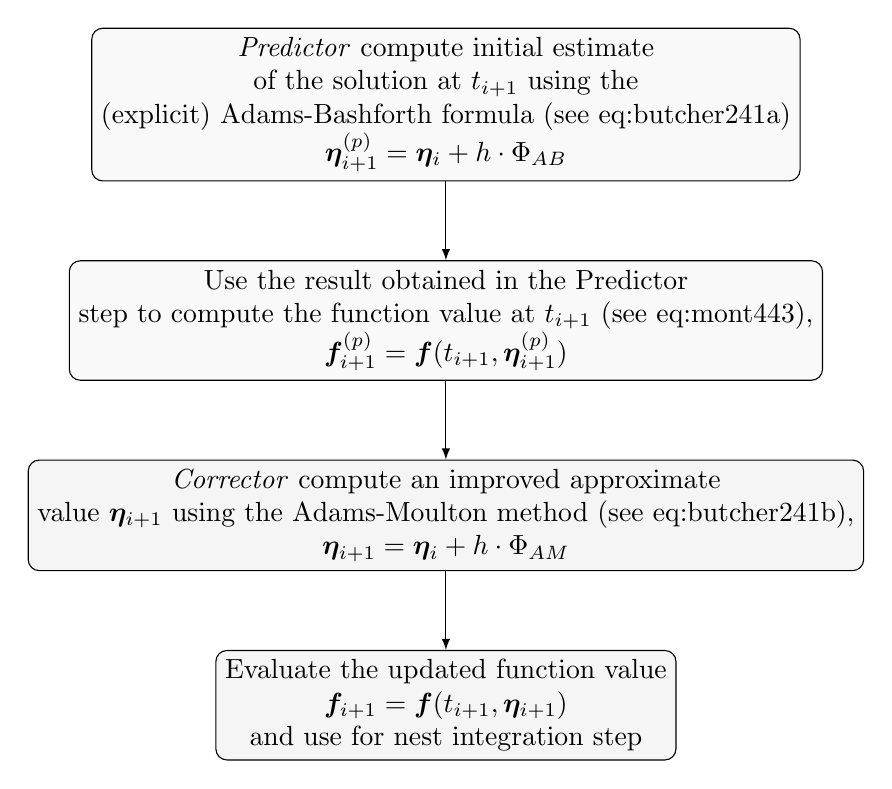
\begin{tikzpicture}[
    every node/.style = {
      draw=black, 
      rounded corners, 
      fill=gray!20,
      minimum width=2cm,
      minimum height=0.5cm,
      align=center},
      every path/.style = {draw, -latex}
    ]

    \node[fill=gray!5] (step1) [] {
        \emph{Predictor} compute initial estimate \\
        of the solution at $t_{i+1}$ using the\\
         (explicit) Adams-Bashforth formula (see \autoref{eq:butcher241a})\\
        $\bm{\eta}^{(p)}_{i+1} = \bm{\eta}_{i} + h \cdot \Phi _{AB}$
      };
    
    \node[fill=gray!5] (step2) [below =of step1] {
        Use the result obtained in the Predictor\\
        step to compute the function value at $t_{i+1}$ (see \autoref{eq:mont443}),\\
        $\bm{f}^{(p)}_{i+1} = \bm{f}(t_{i+1}, \bm{\eta}^{(p)}_{i+1})$
    };
    
    \node[fill=gray!8] (step3) [below =of step2] {
        \emph{Corrector} compute an improved approximate\\
        value $\bm{\eta}_{i+1}$ using the Adams-Moulton method (see \autoref{eq:butcher241b}),\\
        $\bm{\eta}_{i+1} = \bm{\eta}_{i} + h \cdot \Phi _{AM}$
    };

    \node[fill=gray!8] (step4) [below =of step3] {
        Evaluate the updated function value\\ 
        $\bm{f}_{i+1} = \bm{f}(t_{i+1}, \bm{\eta}_{i+1})$\\
        and use for nest integration step
    };

    \draw (step1) -- (step2);
    \draw (step2) -- (step3);
    \draw (step3) -- (step4);

\end{tikzpicture}

  \caption{Schematic representation of the \emph{Predictor-Corrector} algorithm using the Adams-Bashforth and Adams-Moulton methods.}
  \label{fig:pece-adams}
\end{figure}

Even though the \gls{pece} algorithms are complicated and difficult to implement, 
they offer increased stability, especially at large stepsizes (\cite{Montenbruck2000}).
Low-order methods are generally more stable even for large stepsizes.

  
According to \cite{Shampine1975}, use of Adams methods are most advantageous for 
problems in which:
\begin{itemize}
    \item function evaluations are expensive,
    \item mnoderate to high accuracy is requested,
    \item many output points are required
\end{itemize}

\cite{Shampine1975}:
The overhead in these codes is rather high, partly because of the methods
and partly because of the features they provide. For example, DE detects
and deals with discontinuities; it detects and deals with moderate stiffness;
it detects and tells the user of severe stiffness; it detects requests for very
high accuracy and switches on propagated roundoff controls; it detects
requests for more accuracy than is possible on the machine being used and
tells the user what is possible; it is, for practical purposes, independent
of the number and location of output points; it monitors the work being
expended; it allows the user to change direction without restarting; and
it is extremely efficient in terms of function evaluations. 

    \subsection{Integrator Validation}\label{sec:integrator-validation}

\info{new subsection}
Checking and validating integrator results is not a straight-forward process, since 
the computation of the complex force field acting on the satellite is required 
(see \autoref{ssec:perturbed-motion}). Some of these forces further depend on 
satellite-specific characteristics (e.g. atmospheric drag, solar radiation 
pressure). Additionally, validation of trajectory extrapolation requires a ``reference'' 
orbit (i.e. reference state results), which may have been computed using a non 
identical set of models, reference frames and algorithms.

To test the integrator designed and implemented for this Thesis, \gls{ids}-published 
(\cite{Willis2016}) \texttt{sp3} files were acquired and used as ``reference'' orbits. 
These orbits are the accumulated results for the satellite state, tabulated at 
equidistant epochs, of the individual analysis centers contributing to the service. 
Hence, they represent state-of-the-art \gls{pod} results using the \gls{doris} 
satellite system.

The test devised to check the integrator proceed as follows:
\begin{enumerate}
  \item Read a state vector off from the sp3 file for an epoch $t$
  \item Extrapolate the state to a later time $t_i$ (prior to the end of sp3 records)
  \item Read the state off from the sp3 file for the epoch $t_i$ and compare 
    with the results obtained from the integrator. Go to (1) and repeat the 
    process.
\end{enumerate}
The force model used within the integrator, does not contain contributions of the 
solar radiation pressure and atmospheric drag. Ocean tidal loading effects on the 
geopotential, are limited to the 11 major tides. All other contributions, are 
computed as described in \autoref{ssec:perturbed-motion}. Handling of the 
transformation between the \gls{itrf} and \gls{gcrf} is described in 
\autoref{ssec:the-celestial-reference-frame}.

The validation test is performed for a time interval of approximately one week, 
starting on 26/08/2022. The satellite mission picked for the test is Jason-3 
(\cite{Bannoura2011}), since this is the mission used later on, to test the 
integrated \gls{pod} process.

Normally, in a \gls{pod} process using the \gls{doris} system, there is no need to 
extrapolate an orbit further than some seconds, after it has been adjusted by the 
inclusion of observations (see \autoref{ch:pod}). Two distinct measurements are made 
every \SI{10}{\sec} and the ground network is dense enough so that at least one 
ground stations is nearly always visible by any \gls{doris}-equipped satellite. 
For the validation process, extrapolation is tested up to time intervals of 
\SI{15}{\minute} to gain a thorough view on the robustness of the implemented 
algorithm (\autoref{fig:sp3-vs-integration-1min}).

\autoref{fig:sp3-vs-integration-1min} depicts the differences in the state vector 
$\bm{y} = \begin{pmatrix}\bm{r} & \bm{v}\end{pmatrix}^T$ between the reference values 
obtained by the \texttt{sp3} file and the ones computed using the integrator with 
an extrapolation interval of \SI{1}{\minute}. Differences in the position range 
between \qtyrange{-2}{2}{\milli\metre} while for the velocity components the 
differences are within \qtyrange{-1e-5}{1e-5}{\meter\per\second}. A diurnal 
signal seems to be present in the latter case, which could be due to unmodeled 
effects of \begin{itemize}
  \item (remaining) ocean tidal constituents, 
  \item solid earth pole tides and ocean pole tides,
  \item solar radiation pressure acting on the satellite,
  \item atmospheric drag
\end{itemize}
\begin{figure}
  \centering
  \includegraphics[height=.4\textheight,keepaspectratio]{intrp.ja3.1min}
  \caption{Integration results of satellite state compared to respective 
    \gls{ids}-distributed sp3 file records. Extrapolation is performed for an 
    interval of \SI{1}{\minute}.}
  \label{fig:sp3-vs-integration-1min}
\end{figure}

\autoref{fig:sp3-vs-integration-3min} depicts the differences in the state vector 
when the integration interval is expanded to \SI{3}{\minute}. Differences in 
position range between \qtyrange{-5}{5}{\milli\metre} while for the velocity 
components the differences are within \qtyrange{-2e-5}{2e-5}{\meter\per\second}. As in the 
case of \SI{1}{\minute} extrapolation (see \autoref{fig:sp3-vs-integration-1min}), 
velocity differences are dominated by a harmonic, diurnal signal and the same can 
be told for the position discrepancies.
\begin{figure}
  \centering
  \includegraphics[height=.4\textheight,keepaspectratio]{intrp.ja3.3min}
  \caption{Integration results of satellite state compared to respective 
    \gls{ids}-distributed sp3 file records. Extrapolation is performed for an 
    interval of \SI{3}{\minute}.}
  \label{fig:sp3-vs-integration-3min}
\end{figure}

Differences when extrapolating for an interval of \SI{15}{\minute} are depicted 
in \autoref{fig:sp3-vs-integration-15min}. In this case, differences in position 
range between \qtyrange{-5}{5}{\centi\metre} while for the velocity components 
the range is \qtyrange{-.1}{.1}{\milli\meter\per\second}
\begin{figure}
  \centering
  \includegraphics[height=.4\textheight,keepaspectratio]{intrp.ja3.15min}
  \caption{Integration results of satellite state compared to respective 
    \gls{ids}-distributed sp3 file records. Extrapolation is performed for an 
    interval of \SI{15}{\minute}.}
  \label{fig:sp3-vs-integration-15min}
\end{figure}

In general, due to the very small magnitude in the discrepancies computed for the 
extrapolated vs the ``reference'' state (see \autoref{fig:sp3-vs-integration-1min}, 
\autoref{fig:sp3-vs-integration-3min} and \autoref{fig:sp3-vs-integration-15min}), 
the design of the algorithm and its implementation seem to be robust, while the 
discrepancies are attributed to either mismodelled, or unmodelled effects.


\chapter{\gls{pod}}\label{ch:pod}
%\iffalse
  \section{Introduction}\label{sec:pod-introduction}

Orbit determination of artificial satellites began in essence in the 1960s. However, 
it wasn't until the 1980s that great advancements were made, facilitated by
a better modeling of the Earth's gravity field and its variations (e.g. tides) and
the large increase in computing capabilities. This enabled orbit determination 
accuracy to increase to the tens-of-centimeter level. This improvement was
motivated and further pushed by the ever-increasing demands of scientists in the 
oceanographic and geodetic communities, in search for centimeter-level accuracy 
in global ocean topography obtained from altimetric satellites (\cite{Tapley2004}).
To-date, \gls{pod} can yield results in the  few-centimeter level.

Orbit determination can be viewed as a special case of a parameter estimation problem, 
where the parameters characterizing the orbit of an Earth orbiting satellite have to be 
determined from observations. Observations are themselfes values of nonlinear functions 
(the so-called \emph{observed functions}, \cite{BeutlerVII}), thus for the solution 
of the problem, initial approximate parameter values are needed (a problem often 
called \emph{initial orbit determination}). Such approximate starting values can be 
obtained in a number of ways (see e.g. \cite{Vallado2001}), including published 
values of preliminary solutions, and will not be considered here. Hence, the \gls{pod}
process is in essence an \emph{orbit improvement} problem.

Apart from the orbital elements or equivalently the state vector, a number of
different parameters have to be considered in a \gls{pod} problem, including
\begin{itemize}
    \item dynamical parameters characterizing the force model, necessary to describe 
        the orbital motion of the satellites,
    \item coordinates of the observing sites in an \gls{ecef} system,
    \item motion of the observing sites (e.g. crustal deformation),
    \item Earth rotation and Earth orientation parameters,
    \item atmosphere parameters defining the tropospheric refraction correction,
    \item parameters defining the ionospheric refraction correction,
    \item technique-specific, hardware and (possibly site-specific) instrumentation
        bias parameters
\end{itemize}
All of these parameters have to be considered and dealt-with (either estimated or 
introduced) in a \gls{pod} analysis scheme. In this thesis, a ``restricted'' problem 
is addressed, often labeled \emph{pure orbit determination}, where coordinates of 
reference observation sites are assumed to known (via their \gls{ecef} position vector).

It is not always possible to describe the entire time period covered by observations 
by one set of initial conditions and dynamic parameters (\cite{BeutlerVII}). Thus,
the period can be split into consecutive \emph{orbital arcs}; an orbital arc is 
thought of as contiguous, limited part of the satellite's trajectory, described by 
exactly one initial state vector and the dynamical parameters. Using short arcs, 
modeling deficiencies can be mitigated (absorbed by the initial state vectors),
but rapidly increases the number of arc-specific parameters, a fact that could lead 
to a considerably weakened solution (\cite{BeutlerVII}). To overcome this problem, 
an alternate method can be used, in which stochastic accelerations are introduced 
(added to the parameter list), with known mean values and variance-covariance matrices.
Not only observation noise but also system noise has to be introduced, and each 
\emph{deterministic} parameter is replaced by a stochastic process (see e.g. \cite{Jaggi2005b} 
and \cite{Jaggi2005a} for a least-squares approach).

\iffalse
The precise orbit determination of LEO, such as Starlette, Stella, and AJISAI is more
demanding than the determination of the LAGEOS orbits, because of:
-a larger sensitivity to the Earth’s gravity field and to its temporal variations,
-a large sensitivity to atmospheric drag models and variations of air density in the
upper atmosphere, (diss_ks_front)

Gauss’s theory, Kalman filters, and so forth, ultimately needed more precise data.
Without improvements in observational instruments, many of the techniques and meth-
ods in this chapter would be of little use.

On the other hand, the stochastic approach (involving or con-
taining a random variable, a chance, or a probability) uses information in addition to
measurements to account for the fact that neither the mathematical models nor the mea-
surements are perfectly known but are corrupted by random processes. The stochastic
approach combines information from the dynamics, uncertainty with the force model,
and the measurement errors to obtain the best estimate possible. This combination is the
basis of estimation.

Even our best theories can’t exactly model the atmosphere, the Earth’s gravity field,
or the satellite’s attitude. Process noise, v, is a mathematical model of the errors in the
system dynamics. Bierman (1977:113) notes that in a general sense, process noise also represents effects of un-
modeled parameters, linearization, and even “effects such as leaky attitude controls or solar
wind.” It quantifies our ability to model accurately the actual dynamics
before and after a given epoch. The effect of process-noise is that the dynamics may introduce measurable error into
the solution. One difficulty is that we often assume the process-noise statistics are ran-
dom. Unfortunately, they’re often systematic errors such as we might expect from an
incomplete gravity model. These errors can be highly correlated with time and not well
approximated by white noise. Closely related is the power-density matrix or the second
moment of the process noise, Q, which is a covariance of acceleration errors induced by
the mathematical modeling of the system dynamics.

The procedure typically involves an iterative least-squares estimation
seeking best ts of selected model parameters and model-predicted satellite
position and velocity to the tracking data along an orbit arc. The predicted
state at each epoch is integrated by using the satellite equations of motion re-
quiring accurate force models.
\fi

    \subsection{Goals of Current Chapter}\label{ssec:pod-goals}
In this section the fundamentals of orbit determination are discussed, focusing on 
two of the most crucial problems:
\begin{itemize}
  \item the derivation, computation and solution of the so called \emph{variational equations}, and 
  \item efficient, robust and precise parameter estimation via a variation of the 
    Kalman filter, labeled \emph{Extended Kalman Filter}
\end{itemize}

Variational equations are a set of differential equations that describe how small changes 
(i.e. perturbations) in initial conditions propagate over time and thus play a important 
role in predicting the satellite's trajectory. For the derivation of these equations, 
a linearization of the (non-linear) equations of motion is needed. Solution of the 
variational equations is coupled with the computation of the \emph{state transition matrix}, 
which relates the perturbed state at one epoch to a perturbed state at a later time and 
can be used to propagate the covariance matrix. Propagating the latter forward in time, 
a prediction can be made of the evolution of uncertainty in the estimate of the satellite's 
state. Formulas and numerical recipes for the linearization, as well as the differential 
equations of the state transition matrix and variational equations are presented. 
The discussion focuses on a hands-on approach, limiting analytical derivations which can be 
found in relevant literature. Equations are presented in matrix form, to enable an 
as much as possible easy translation to source code, and special care is taken to 
single out and exploit features, equations and particularities that can be used to derive 
a more efficient and/or robust algorithmic design.

Subsequently, the problem of parameter estimation is considered. There are two major 
methodologies that come into play in \gls{pod} problems, the method of \emph{Least Squares} 
and the extended family of filters called \emph{Kalman filters} and variations. 
For the current thesis, the latter methodology was used and more specifically the 
\emph{Extended Kalman filter} to derive a robust estimator. Computational aspects of the 
methodology and the implementation are discussed, as well as advantages and shortcomings.

Since a discussion on the input data for the \gls{pod} problem considered in this Thesis 
is not yet touched upon, the computation of \emph{observation equations} (needed in the 
estimation process) is not thoroughly presented here; this issue will be revisited once the 
basics of the DORIS system are presented (??see chapter 5??).

  \section{Linearization}\label{sec:pod-linearization}

In a \gls{pod} problem, both the dynamics and the measurements involve significant 
nonlinear relationships. For both the trajectory and the observation models, a large 
number of partial derivatives have to be computed for a rigorous linearization. These, 
according to \cite{Montenbruck2000} can be divided into four different categories:
\begin{description}
  \item[The State Transition Matrix] $\bm{\Phi}(t,t_0)$, which maps deviations in the 
    state vector from an epoch $t_0$ to a later time $t$, and is given by
    \begin{equation}\label{eq:mont71}
      \bm{\Phi} (t,t_0) = \left(
          \frac{\partial \bm{y}(t)}{\partial \bm{y}(t_0)} 
        \right) _{(6 \times 6)}
    \end{equation}

  \item[The Sensitivity Matrix] $\bm{S}(t)$, which describes the dependence of the 
    orbit on the dynamical parameters $p_i$ with $i=1,2,\dots ,n_p$ and is formed 
    by the respective partial derivatives of the state with respect to the force 
    model, 
    \begin{equation}\label{eq:mont72}
      \bm{S} (t) = \left(
          \frac{\partial \bm{y}(t)}{\partial \bm{p}} 
        \right) _{(6 \times n_p)}
        = \begin{pmatrix} 
          \frac{\partial x(t)}{\partial p_1} & \frac{\partial x(t)}{\partial p_2} & \dots & \frac{\partial x(t)}{\partial p_n} \\
          \frac{\partial y(t)}{\partial p_1} & \frac{\partial y(t)}{\partial p_2} & \dots & \frac{\partial y(t)}{\partial p_n} \\
          \frac{\partial z(t)}{\partial p_1} & \frac{\partial z(t)}{\partial p_2} & \dots & \frac{\partial z(t)}{\partial p_n} \\
          \frac{\partial \dot{x}(t)}{\partial p_1} & \frac{\partial \dot{x}(t)}{\partial p_2} & \dots & \frac{\partial \dot{x}(t)}{\partial p_n} \\
          \frac{\partial \dot{y}(t)}{\partial p_1} & \frac{\partial \dot{y}(t)}{\partial p_2} & \dots & \frac{\partial \dot{y}(t)}{\partial p_n} \\
          \frac{\partial \dot{z}(t)}{\partial p_1} & \frac{\partial \dot{z}(t)}{\partial p_2} & \dots & \frac{\partial \dot{z}(t)}{\partial p_n}
      \end{pmatrix}
    \end{equation}

  \item[Partials of the measurements with respect to the state vector], which given 
    an observation $z$  at some instant $t$, is given by
    \begin{equation}\label{eq:mont73}
      \left( \frac{\partial z}{\partial \bm{y}(t)} \right) _{(1 \times 6)}
    \end{equation}, and

  \item[Partials with respect to measurement model parameters], which given the observation 
    model parameters $q_i$ for $i=1,2, \dots ,n_q$, given by 
    \begin{equation}\label{eq:mont74}
       \left( \frac{\partial z}{\partial \bm{q}} \right) _{(1 \times n_q)}
    \end{equation}

\end{description}

Note that from \autoref{eq:mont71}, the dependence of an individual observation $z$ 
on the initial state $\bm{y}(t_0)$ is
\begin{equation}
  \frac{\partial z}{\partial \bm{y}(t_0)} = 
    \frac{\partial z}{\partial \bm{y}(t)}\frac{\partial \bm{y}(t)}{\partial \bm{y}(t_0)} 
    = \frac{\partial z}{\partial \bm{y}(t)} \bm{\Phi} (t,t_0)
\end{equation}
and from \autoref{eq:mont72}
\begin{equation}
  \frac{\partial z}{\partial \bm{p}} = 
    \frac{\partial z}{\partial \bm{y}(t)}\frac{\partial \bm{y}(t)}{\partial \bm{p}}
    = \frac{\partial z}{\partial \bm{y}(t)} \bm{S} (t)
\end{equation}

Analytical computation of the partial derivatives is tedious, cumbersome and an 
error prone procedure. However, it constitutes an essential part of orbit determination 
and have a noticable impact on the achieved performance and convergence speed 
(\cite{Montenbruck2000}).

The orbit determination problem, can in the general case be described by the 
1\textsuperscript{st} order \gls{ode} system for the dynamics accompanied with 
the observation functions
\begin{align}
  \bm{\dot{Y}} &= \bm{F}(t, \bm{Y}) \label{eq:tapley421} \\
  \bm{Z}_i     &=  G(t_i, \bm{Y}_i) + \bm{\epsilon}_i \label{eq:tapley422}
\end{align}
where $\bm{y}$ is the state vector and $\bm{z}_i$ is a $p-$dimensional set of 
observations, for $i=1,2,\dots ,l$. If a sufficiently precise reference (initial) 
trajectory $\bm{y}^{*}$ is available, then the actual, ``true'' trajector $\bm{y}$ 
can be expanded in a Taylor series about this reference trajectory at each point 
in time. Truncating higher order terms, the deviation in state from the 
reference trajectory can be described by a set of linear differential equations 
with time-dependent coefficients. The same procedure can be used in \autoref{eq:tapley422} 
to obtain a linear relation between the observation deviation and the state deviation.
In this way, the original, non-linear orbit determination problem is transformed 
to a linear proble, in which the deviation from some reference solution must be 
determined.
If $\bm{y}$ denotes the state deviation vector and $\bm{z}$ the observation deviation 
vector, then
\begin{equation}
  \begin{aligned}
    \bm{y}(t) &= \bm{Y}(t) - \bm{Y}^{*}(t) \\
    \bm{z}(t) &= \bm{Z}(t) - \bm{Z}^{*}(t)
  \end{aligned}
\end{equation}
so that
\begin{equation}\label{eq:tapley424}
  \dot{\bm{y}}(t) = \dot{\bm{Y}}(t) - \dot{\bm{Y}}^{*}(t)
\end{equation}
Expanding \autoref{eq:tapley421} and \autoref{eq:tapley422} in a Taylor's series 
about the reference trajectory, leads to (\cite{Tapley2004})
\begin{equation}\label{eq:tapley425a}
  \begin{aligned}
  \bm{\dot{Y}}(t) &= \bm{F}(t, \bm{Y}) \\
                  &= \bm{F}(t, \bm{Y}^{*}) + 
                  \frac{\partial \bm{F}(t, \bm{Y})}{\partial \bm{Y}^{*}(t)} 
                  \left( \bm{Y}(t) - \bm{Y}^{*}(t) \right) 
                  + \mathcal{O}\left( \bm{Y}(t) - \bm{Y}^{*}(t) \right)
  \end{aligned}
\end{equation}
and
\begin{equation}\label{eq:tapley425b}
  \begin{aligned}
  \bm{Z}_i &= \bm{G}(t_i, \bm{Y}_i) + \epsilon _i \\ 
           &= \bm{G}(t, \bm{Y}^{*}_{i}, t_i) 
           + \frac{\partial \bm{G}}{\partial \bm{Y}^{*}}\at{i} 
           \left( \bm{Y}(t_i) - \bm{Y}^{*}(t_i) \right) 
           + \mathcal{O}\left( \bm{Y}(t_i) - \bm{Y}^{*}(t_i) \right) 
           + \epsilon _i
  \end{aligned}
\end{equation}
where the partials are evaluated on the reference solution, $\bm{Y}^{*}(t)$ can be 
obtained by integrating \autoref{eq:tapley421} and $\mathcal{O}$ indicate terms 
containing products of the difference $\bm{Y}(t) - \bm{Y}^{*}(t)$ higher than the 
first term. Given that these terms are sufficiently small to be neglecting and using 
$ \bm{\dot{Y}}^{*} = \bm{F}(t, \bm{Y}^{*})$, \autoref{eq:tapley425a} and 
\autoref{eq:tapley425b} can be written as
\begin{equation}\label{eq:tapley426}
  \begin{aligned}
    \dot{\bm{y}}(t) &= A(t) \bm{x}(t) \\
    \bm{z}_i &= H_i \bm{x}_i + \epsilon _i
  \end{aligned}
\end{equation}
where 
\begin{equation}
  A(t) = \frac{\partial F (t)}{\partial \bm{Y}(t)}\at{\bm{X}^{*}} 
  \text{ and }
  H_i = \frac{\partial G}{\partial \bm{Y}}\at{\bm{X}^{*}_i}
\end{equation}

    \subsection{State Transition Matrix}\label{ssec:pod-state-transition-matrix}

\autoref{eq:tapley426a} represents a system of linear differential equations with 
time-dependent coefficients (notice that the matrix $A$ in \autoref{eq:tapley426c} 
is derived from a particular solution of $\dot{\bm{y}}=\bm{f}(t,\bm{y})$, generated 
with the initial conditions $\bm{y}(t_0)=\bm{y}^{*}_{0}$). The general solution for 
this system can be expressed as 
\begin{equation}\label{eq:tapley427}
    \delta \bm{y}(t) = \Phi (t,t_k) \delta \bm{y}_k
\end{equation}
with $\delta \bm{y}_k \equiv \delta \bm{y}(t_k)$
Differentiating \autoref{eq:tapley427} and noting that $\delta \bm{y}_k$ is constant, 
gives
\begin{equation}\label{eq:tapley429}
    \delta \dot{\bm{y}}(t) = \dot{\Phi} (t,t_k) \delta \bm{y}_k
\end{equation}
and using \autoref{eq:tapley426a} and \autoref{eq:tapley427}, the \gls{ode} system 
\begin{equation}\label{eq:tapley4210}
    \begin{aligned}
        \dot{\Phi} (t,t_k) &= A(t) \Phi (t,t_k) \\
        \Phi (t_k,t_k) &= \bm{I}
    \end{aligned}
\end{equation}
The great advantage of this formulation, is that it allows the solution $\delta \bm{y}(t)$ 
to be expressed in terms of the unknown initial state $\delta \bm{y}_k$. Hence, the 
state transition matrix enables relating observations made at different times.
    
The \gls{ode} system for the state transition matrix \autoref{eq:tapley429} 
is prefered against a direct solution of $\delta \bm{y}(t)$ from the system
\autoref{eq:tapley426a} for computational reasons, \cite{Tapley2004}.

\cite{Montenbruck2000} give the formulae for forming the state transition matrix 
using orbital elements and the associated partials with respect to the state vector.
\cite{Battin1999} uses the fact that $\Phi$ is a \emph{sympletic} matrix, to obtain 
an analyticaly its inverse.

    \subsection{The Observation Equations}\label{ssec:pod-observation-equations}

\autoref{eq:tapley426b} involves an unknown state vector $\delta \bm{y}_i$ related 
to the observation set $\bm{z}_i$. The state transition matrix can be used to relate 
all observation with the state at a single epoch. For each set, \autoref{eq:tapley426b} 
($\bm{\delta z}_i = H_i \delta \bm{y}_i + \epsilon _i$) can be written as 
\begin{equation}\label{eq:tapley4237}
    \bm{\delta z}_i = H_i \Phi (t_i,t_k) \delta \bm{y}_k + \epsilon _i
\end{equation}
where \autoref{eq:tapley427} was used, and subsequently in matrix form 
\begin{equation}\label{eq:tapley4239}
    \bm{\delta z} = \bar{H} \delta \bm{y}_k + \bm{\epsilon}
\end{equation}
with
\begin{equation}
    \bm{\delta z} \equiv \begin{pmatrix}\bm{\delta z}_1 \\ \bm{\delta z}_2 \\ \vdots \\ \bm{\delta z}_l \end{pmatrix} 
    \text{ , }
    \bar{H} \equiv \begin{pmatrix}H_1 \Phi (t_1,t_k) \\ H_2 \Phi (t_2,t_k) \\ \vdots \\ H_l \Phi (t_l,t_k)\end{pmatrix} 
    \text{ and }
    \bm{\delta z} \equiv \begin{pmatrix}\bm{\epsilon}_1 \\ \bm{\epsilon}_2 \\ \vdots \\ \bm{\epsilon}_l \end{pmatrix} 
\end{equation}

  \section{The Kalman Filter}\label{sec:pod-kalman-filter}

In this section, the sequential estimation algorithm referred to as the 
\emph{Kalman filter} is discussed, with emphasis on its application on the orbit 
determination problem. A more thorough discussion on the sequential estimation 
techniques can be found at \cite{Gelb1974}, while \cite{Montenbruck2000} and 
\cite{Tapley2004} describe the filter's application and variations thereof for 
\gls{pod}. One important advantage of the Kalman filter is that the matrix to be 
inverted will be of the same dimension as the observation vector, which means 
that given that the observations can be processed one at a time, only scalar 
divisions will be required to obtain the estimate of $\delta \bm{y}(t_k)$. For the 
rest of this section, the notation $\bm{y}_k$ will be used to denote the value 
$\delta \bm{y}(t_k)$ to reduce complexity and follow relevant literature in the 
field.

Given that an estimate $\hat{\bm{y}}_j$ and the associated covariance matrix $\bm{P}_j$ 
are available at a given epoch $t_j$, the state and its variance-covariance matrix can 
be propagated according to
\begin{equation}\label{eq:tapley471}
    \begin{aligned}
        \bar{\bm{y}}_k &= \phi (t_k, t_j) \hat{\bm{y}}_j \\
        \bar{\bm{P}}_k &= \phi (t_k, t_j) \bm{P}_j \phi ^{T}(t_k, t_j)
    \end{aligned}
\end{equation}
This step of the algorithm, is often called the \emph{time update} step. 
Assuming that an observation is available at $t_k$
\begin{equation}\label{eq:tapley472}
    \bm{z}_k = \tilde{H}_k \bm{y}_k + \bm{\epsilon}_k
\end{equation}
with $E [\bm{\epsilon}_k] = \bm{0}$ and  
$E [\bm{\epsilon}_k \bm{\epsilon}^{T}_k] = \bm{R}_k \delta _{kj}$, it can be 
shown (see \cite{Tapley2004}) that:
\begin{align}
    K_k &= \bar{\bm{P}}_k \tilde{H}^{T}_{k} 
        \left( \tilde{H}_{k} \bar{\bm{P}}_k \tilde{H}^{T}_{k} 
            + \bm{R}_k \right)^{-1} \label{eq:tapley4711} \\
    \bm{P}_k &= \left( \bm{I} - \bm{K}_k \tilde{H}_{k} \right) \bar{\bm{P}}_k 
        \label{eq:tapley4712} \\
    \hat{\bm{y}}_k &= \bar{\bm{y}}_k + \bm{K}_k 
        \left( \bm{z}_k - \tilde{H}_{k} \bar{\bm{y}}_k \right) \label{eq:tapley4716}
\end{align}
\autoref{eq:tapley4711}, \autoref{eq:tapley4712} and \autoref{eq:tapley4716} are 
collectively labeled the \emph{measurement update} step. The matrix $\bm{K}$ is 
called the \emph{(Kalman) gain matrix}.
The above equations can be used in a recursive fashion to compute the estimate of 
$\hat{\bm{y}}_k$, incorporating the observation $\bm{z}_k$. A flowchart of the 
process is depicted in \autoref{fig:kalman-pod}.

\begin{figure}
    \centering
    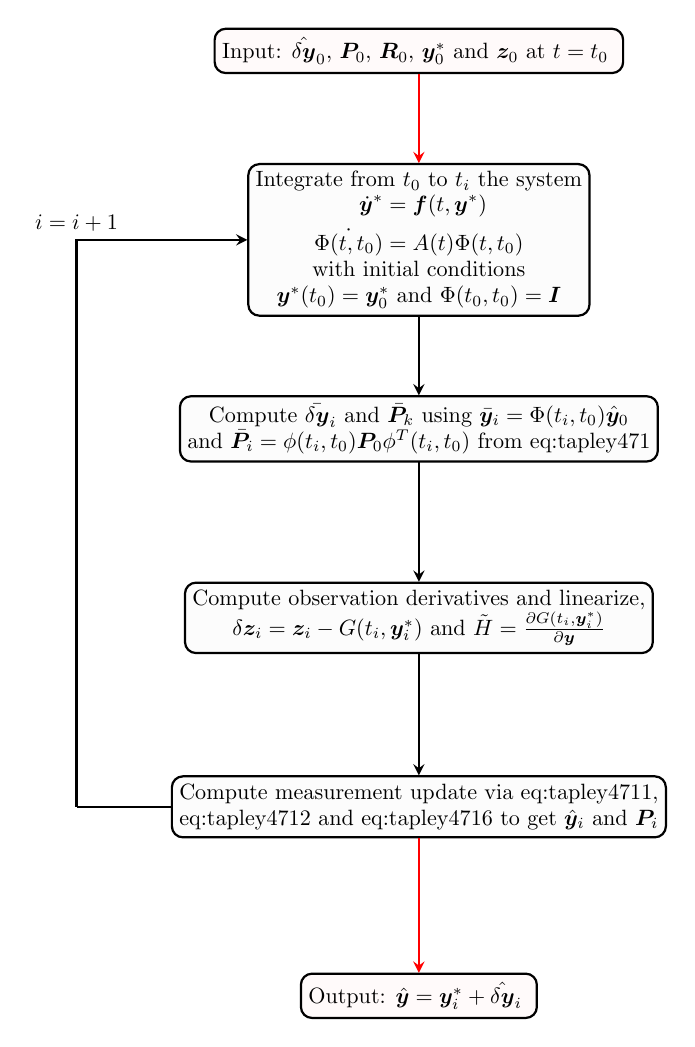
\begin{tikzpicture}[align=center, thick,scale=0.8, every node/.style={scale=0.8}]

    \node[rectangle,
        draw,
        text centered,
        rounded corners,
        minimum height=2em,
        fill=red!2] 
    (input) at (0,0) {
        Input: $\hat{\delta \bm{y}}_{0}$, $\bm{P}_{0}$, $\bm{R}_0$, $\bm{y}^{*}_{0}$
        and $\bm{z}_0$ at $t=t_0$
    };

    \node[rectangle,
        draw,
        text centered,
        rounded corners,
        minimum height=2em,
        align=center,
        fill=gray!2] 
    (integrate) at (0,-3) {
        Integrate from $t_0$ to $t_i$ the system\\
        $
            \begin{aligned}
                \dot{\bm{y}}^{*} &= \bm{f}(t, \bm{y}^{*}) \\
                \dot{\Phi (t,t_0)} &= A(t) \Phi(t,t_0)
            \end{aligned}
        $\\
        with initial conditions\\
        $\bm{y}^{*}(t_0) = \bm{y}^{*}_0$ and $\Phi (t_0,t_0) = \bm{I}$
    };

    \node[rectangle,
        draw,
        text centered,
        rounded corners,
        minimum height=2em,
        align=center,
        fill=gray!2] 
    (approx) at (0,-6) {
        Compute $\bar{\delta \bm{y}}_{i}$ and $\bar{\bm{P}}_k$ using 
        $\bar{\bm{y}}_i = \Phi (t_i, t_0) \hat{\bm{y}}_0$ \\
        and $\bar{\bm{P}}_i = \phi (t_i, t_0) \bm{P}_0 \phi ^{T}(t_i, t_0)$ 
        from \autoref{eq:tapley471}
    };
    
    \node[rectangle,
        draw,
        text centered,
        rounded corners,
        minimum height=2em,
        align=center,
        fill=gray!2] 
    (obs) at (0,-9) {
        Compute observation derivatives and linearize,\\
        $\delta \bm{z}_i = \bm{z}_i - G(t_i, \bm{y}^{*}_i)$ and 
        $\tilde{H} = \frac{\partial G(t_i, \bm{y}^{*}_i)}{\partial \bm{y}}$
    };

    \node[rectangle,
        draw,
        text centered,
        rounded corners,
        minimum height=2em,
        align=center,
        fill=gray!2] 
    (upd) at (0,-12) {
        Compute measurement update via \autoref{eq:tapley4711},\\
        \autoref{eq:tapley4712} and \autoref{eq:tapley4716} to get $\hat{\bm{y}}_i$ and $\bm{P}_i$
    };

    \node[rectangle,
        draw,
        text centered,
        rounded corners,
        minimum height=2em,
        fill=red!2] 
    (output) at (0,-15) {
         Output: $\hat{\bm{y}} = \bm{y}^{*}_{i} + \hat{\delta \bm{y}}_{i}$
    };

    \draw [-stealth, thick, red] (input) -- (integrate);
    \draw [-stealth, thick] (integrate) -- (approx);
    \draw [-stealth, thick] (approx) -- (obs);
    \draw [-stealth, thick] (obs) -- (upd);
    \draw [thick] (upd.west) -- ($(upd.west)-(1.5,0)$);
    \draw [-stealth, thick] ($(upd.west)-(1.5,0)$) |- (integrate.west) node[midway, above]{$i = i + 1$}; 
    \draw [-stealth, thick, red] (upd) -- (output);

\end{tikzpicture}
    \caption{Flowchart of the Kalman filter algorithm for orbit determination.}
    \label{fig:kalman-pod}
\end{figure}

Note that the differential equations for the state transition matrix are 
reinitialized at each observation epoch. If observations are introduced as 
scalars, and more than one measurements are available at each epoch, $\Phi (t_i,t_i)$ 
would be set to the unity matrix $\Phi (t_i,t_i) = \bm{I}$ after processing the first 
observation in the epoch, and $\bm{P}$ and $\hat{\bm{y}}$ would only be time updated 
at the next observation epoch $i+1$.

\subsection{Filter Shortcomings}\label{ssec:pod-kalman-filter-shortcomings}
One disadvantage of the sequential algorithm presented here, lies in the fact
that if the true state and the reference state are not close together then the 
linearization assumption leading to \autoref{eq:tapley426} may not be valid and 
the estimation process may diverge (\cite{Tapley2004}). To overcome this problem, 
the \emph{Extended Kalman Filter} algorithm (\autoref{sec:pod-extended-kalman-filter}) 
was used in this Thesis.

Yet another disadvantage is that the state estimation error covariance matrix may 
approach zero as the number as the number of observations becomes large. As 
$\bm{P}_k \to \bm{0}$, gain also approaches zero $\bm{K} \to \bm{0}$, and the 
estimation procedure will become insensitive to further observations. Consequently, 
the estimate will diverge due to either errors introduced in the linearization 
procedure, computational errors, or errors due to an incomplete mathematical model. 
To overcome this problem, process noise often is added to the state propagation 
equations (\cite{Tapley2004}).

In addition to these two problems, the Kalman filter may diverge because of
numerical difficulties associated with the covariance measurement update, given
by \autoref{eq:tapley4712} (\cite{Tapley2004}). This can be the case if the 
covariance matrix loses its properties of symmetry and become non-positive definite 
due to roundoff error (this pitfal is especially possible when a large a priori 
covariance is reduced by the incorporation of very accurate observation data). 
An alternative equation to \autoref{eq:tapley4712} is to use the more numerically 
stable formula introduced by \emph{Bucy} and \emph{Joseph}, which reads
\begin{equation}\label{eq:tapley4719}
    \bm{P}_k = \left( \bm{I} - \bm{K}_k \tilde{\bm{H}} \right) \bar{\bm{P}}_k
    \left( \bm{I} - \bm{K}_k \tilde{\bm{H}} \right)^{T} 
    + \bm{K}_k \bm{R}_k \bm{K}^{T}_k
\end{equation}
More information and a detailed discussion on the stability of relevant approaches 
can be found in \cite{Bierman1977}.

  \section{The Extended Kalman Filter}\label{sec:pod-extended-kalman-filter}

To address the problem of growing the errors due to higher order terms that are 
ignored in the sequential Kalman filter (see \autoref{ssec:pod-kalman-filter-shortcomings}), 
an extended form of the algorithm can be used, labeled the \emph{Extended Kalman Filter}.
The advantage of this approach is that convergence (to the best estimate) is 
accelerated because of the reduced linearization errors. The major disadvantage 
of the extended sequential algorithm is that the differential equations for the 
reference trajectory must be reinitialized after each observation is processed.
A flowchart of the algorithm is depicted in \autoref{fig:efk-pod}.

The primary difference between the clasic formulation and the extended algorithm 
is that the reference trajectory for the extended Kalman filter is updated 
after each observation to reflect the best estimate of the true trajectory. E.g., 
after processing the $k$\textsuperscript{th} observation, the computed best estimate 
is used to provide a new initial condition for the reference orbit,
\begin{equation}\label{eq:tapley4728}
    \bm{y}^{*}_{k, new} = \hat{\bm{y}}_k = \bm{y}^{*}_k + \hat{\delta \bm{y}}_k
\end{equation}

Note that using $\hat{\bm{y}}_k$ as the reference orbit, implies that $\hat{\delta \bm{y}}_k=\bm{0}$ 
and thus $\bar{\delta \bm{y}}_{k+1}=\bm{0}$. The integration for the reference 
trajectory and the state transition matrix is reinitialized at each observation 
epoch, and the equations are integrated forward from $t_k$ to $t_{k+1}$. After 
the time update step, the best estimate can be computed as 
\begin{equation}
    \hat{\delta \bm{y}}_{k+1} = K_{k+1} \bm{y}_{k+1}
\end{equation}
with $K_{k+1}$ and $\bm{y}_{k+1}$ computed based on the updated reference orbit.
The process of incorporating the estimate at each observation point into the 
reference trajectory for propagating to the next observation epoch leads to
the reference trajectory being the prediction of the estimate of the nonlinear state 
(\cite{Tapley2004}), e.g. $\bm{y}^{*}_{t} = \hat{\bm{y}}(t)$.

When implementing the extended Kalman filter for applications demanding high accuracy, 
care must be taken when updating the reference orbit at the begining of the 
processing. Often, the update is omitted for the first few observations, especially 
if these contain significant noise. After a few observations have been processed, 
the estimates of $\hat{\delta \bm{y}}$ will stabilize, and the trajectory update step 
can be added to the process (\cite{Tapley2004}).

\begin{figure}
    \centering
    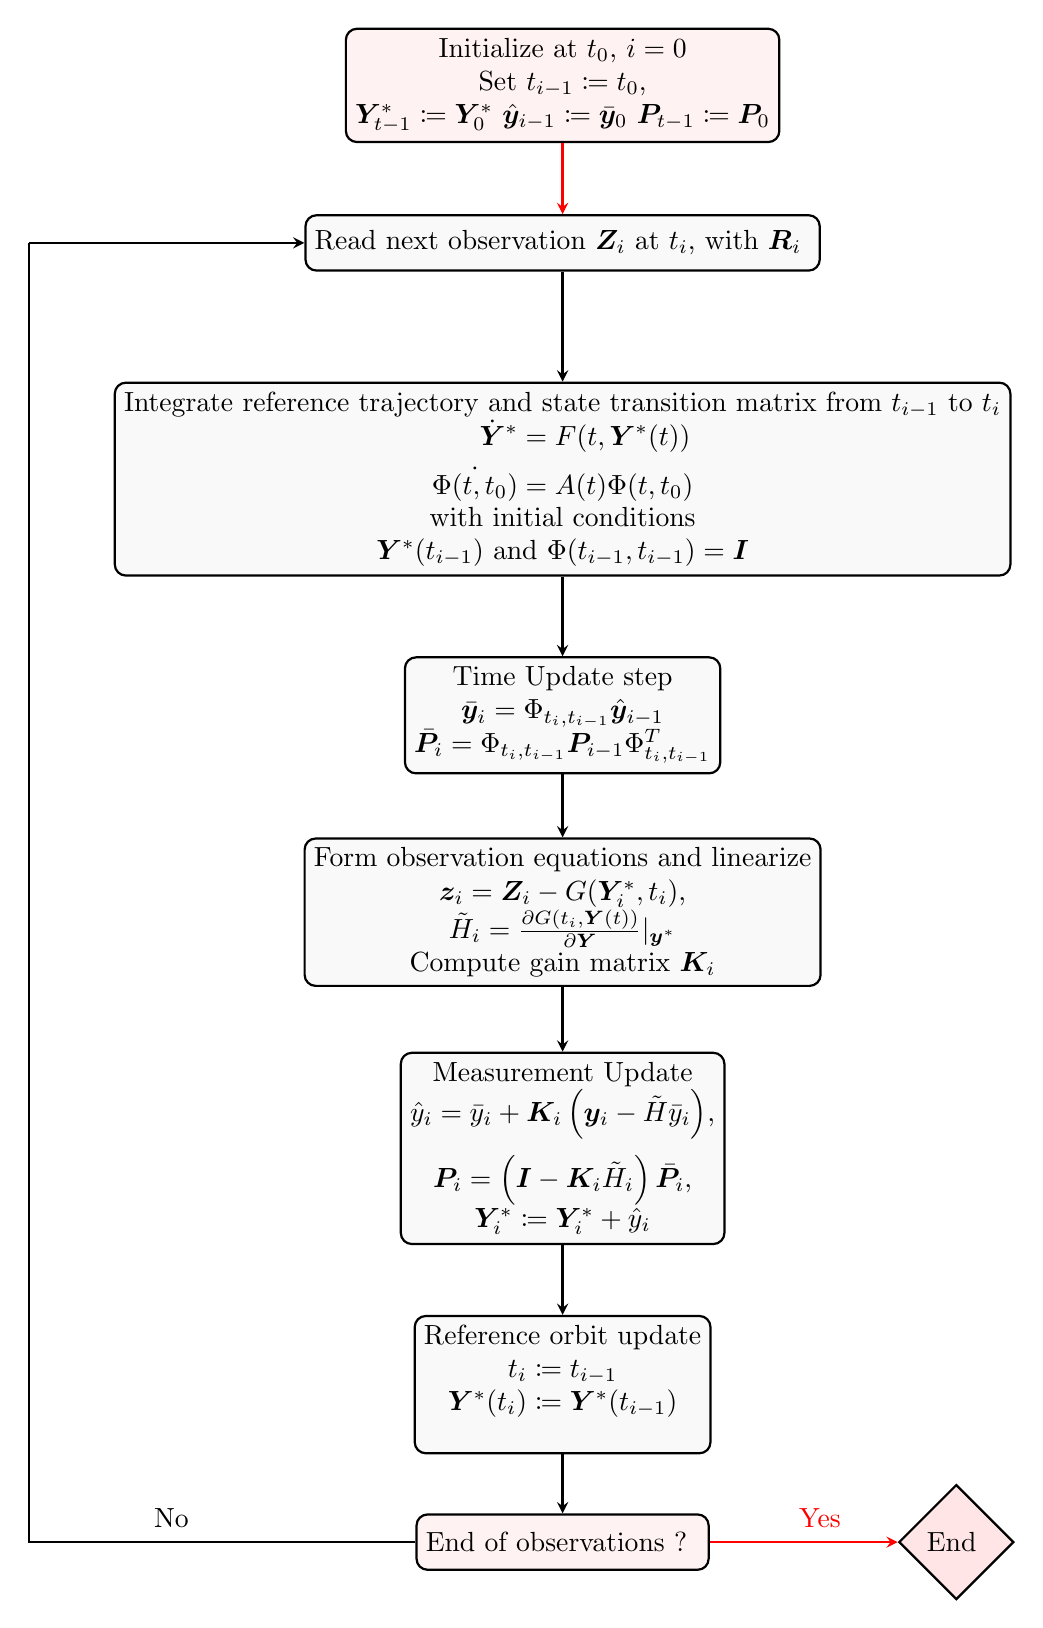
\begin{tikzpicture}[align=center, scale=1.0, every node/.style={scale=1.0}]

    \node[rectangle,
        draw,
        text centered,
        rounded corners,
        minimum height=2em,
        align=center,
        thick,
        fill=red!5] 
    (init) at (0,0) {
        Initialize at $t_0$, $i = 0$\\
        Set $t_{i-1} \coloneqq t_0$,\\
        $\bm{Y}^{*}_{t-1} \coloneqq \bm{Y}^{*}_{0}$
        $\hat{\bm{y}}_{i-1} \coloneqq \bar{\bm{y}}_0$
        $\bm{P}_{t-1} \coloneqq \bm{P}_{0}$
    };

    \node[rectangle,
        draw,
        text centered,
        rounded corners,
        thick,
        minimum height=2em,
        align=center,
        fill=gray!5] 
    (readobs) at (0,-2) {
        Read next observation $\bm{Z}_i$ at $t_i$, with $\bm{R}_{i}$
    };

    \node[rectangle,
        draw,
        text centered,
        rounded corners,
        minimum height=2em,
        align=center,
        thick,
        fill=gray!5] 
    (integrate) at (0,-5) {
        Integrate reference trajectory and state transition matrix from 
        $t_{i-1}$ to $t_i$\\
        $
        \begin{aligned}
            \dot{\bm{Y}}^{*} &= F(t, \bm{Y}^{*}(t)) \\
            \dot{\Phi (t,t_0)} &= A(t) \Phi(t,t_0)
        \end{aligned}
        $\\
        with initial conditions\\
        $\bm{Y}^{*}(t_{i-1})$ and $\Phi (t_{i-1},t_{i-1}) = \bm{I}$
    };
    
    \node[rectangle,
        draw,
        text centered,
        rounded corners,
        minimum height=2em,
        align=center,
        thick,
        fill=gray!5] 
    (tupd) at (0,-8) {
        Time Update step\\
        $\bar{\bm{y}}_i = \Phi _{t_i,t_{i-1}}  \hat{\bm{y}}_{i-1}$\\
        $\bar{\bm{P}}_i = \Phi _{t_i,t_{i-1}} \bm{P}_{i-1} \Phi ^{T}_{t_i,t_{i-1}}$
    };

    \node[rectangle,
        draw,
        text centered,
        rounded corners,
        minimum height=2em,
        align=center,
        thick,
        fill=gray!5] 
    (obs) at (0,-10.5) {
        Form observation equations and linearize\\
        $\bm{z}_i = \bm{Z}_i - G(\bm{Y}^{*}_i, t_i)$,\\
        $\tilde{H}_i = \frac{\partial G(t_i, \bm{Y}(t))}{\partial \bm{Y}}\at{\bm{y}^{*}}$\\
        Compute gain matrix $\bm{K}_i$
    };

    \node[rectangle,
        draw,
        text centered,
        rounded corners,
        minimum height=2em,
        align=center,
        thick,
        fill=gray!5] 
    (mupd) at (0,-13.5) {
        Measurement Update\\
        $\hat{y}_i = \bar{y}_i + \bm{K}_i \left( \bm{y}_i - \tilde{H} \bar{y}_i \right)$,\\ \\
        $\bm{P}_i = \left( \bm{I} - \bm{K}_i \tilde{H}_i \right) \bar{\bm{P}}_i$,\\
        $\bm{Y}^{*}_i \coloneqq \bm{Y}^{*}_i + \hat{y}_i$
    };

    \node[rectangle,
        draw,
        text centered,
        rounded corners,
        minimum height=2em,
        align=center,
        thick,
        fill=gray!5] 
    (roupd) at (0,-16.5) {
        Reference orbit update\\
        $t_i \coloneqq t_{i-1}$\\
        $\bm{Y}^{*}(t_i) \coloneqq \bm{Y}^{*}(t_{i-1})$\\
    };

    \node[rectangle,
        draw,
        text centered,
        rounded corners,
        minimum height=2em,
        thick,
        fill=red!5] 
    (more) at (0,-18.5) {
        End of observations ?
    };
    
    \node[diamond,
        draw,
        minimum height=0.5em,
        thick,
        fill=red!10] 
    (end) at (5,-18.5) {
        End
    };

    \draw [-stealth, thick, red] (init) -- (readobs);
    \draw [-stealth, thick] (readobs) -- (integrate);
    \draw [-stealth, thick] (integrate) -- (tupd);
    \draw [-stealth, thick] (tupd) -- (obs);
    \draw [-stealth, thick] (obs) -- (mupd);
    \draw [-stealth, thick] (mupd) -- (roupd);
    \draw [-stealth, thick] (roupd) -- (more);
    \draw [thick] (more.west) -| ($(readobs.west)-(3.5,0)$);
    \node[] (no) at ($(more.west)-(3.1,-.3)$) {No};
    \draw [-stealth, thick] ($(readobs.west)-(3.5,0)$) -- (readobs);
    \node[red] (yes) at ($(more.east)-(-1.4,-.3)$) {Yes};
    \draw [-stealth, thick, red] (more) -- (end);
    %\draw [-stealth, thick] ($(upd.west)-(1.5,0)$) |- (integrate.west) node[midway, above]{$i = i + 1$}; 
    %\draw [-stealth, thick, red] (upd) -- (output);

\end{tikzpicture}
    \caption{Flowchart of the Extended Kalman filter algorithm for orbit determination.}
    \label{fig:efk-pod}
\end{figure}
  \section{Variational Equations}\label{sec:pod-variational-equations}

For application with high accuracy demands, the state transition matrix should include 
terms at least the major perturbations. That is, the initial value problem should be 
expanded to include differential equations to account for perturbed motion. An 
analytical solution of this problem is close to impossible, thus this extended  
formulation should be solved for numerically. The added differential equations (to 
the state transition matrix system) are labeled \emph{variational equations}.
Aside from the increased accuracy that may be obtained by accounting for perturbations, the
concept of the variational equations offers the advantage that it is not limited to the
computation of the state transition matrix, but may also be extended to the treatment
of partial derivatives with respect to force model parameters (\cite{Montenbruck2000}).

\subsection{Differential Equations for the State Transition Matrix}\label{ssec:pod-state-transition-ode}
Denoting the state vector as $\bm{y}(t) = \begin{pmatrix}\bm{r}(t) & \bm{v}(t) \end{pmatrix}^{T}$, 
the differential equation, which describes the change of the state transition matrix 
with time in a first-order \gls{ode} 
\begin{equation}\label{eq:mont738}
    \frac{d \bm{y}(t)}{d t} = \bm{f}(t,\bm{y}(t)) = 
        \begin{pmatrix}\bm{v}(t)\\\bm{a}(t,\bm{r},\bm{v})\end{pmatrix}
\end{equation}
An differentiating with respect to $\bm{y}(t_0)$ gives
\begin{equation}
    \frac{\partial}{\partial \bm{y}(t_0)} \left( \frac{d \bm{y}(t)}{d t} \right) 
        = \frac{\partial \bm{f}(t,\bm{y}(t))}{\partial \bm{y}(t_0)} 
        = \frac{\partial \bm{f}(t,\bm{y}(t))}{\partial \bm{y}(t)}\frac{\partial \bm{y}(t)}{\partial \bm{y}(t_0)}
\end{equation}
Since the state transition matrix $\Phi (t,t_0)$ is given by
\begin{equation}\label{eq:mont740}
    \Phi (t,t_0) = \frac{\partial \bm{y}(t)}{\partial \bm{y}(t_0)}
\end{equation}
its derivative can be computed from
\begin{equation}\label{eq:mont7412}
    \begin{aligned}
        \frac{d}{dt} \Phi (t,t_0) & = \frac{\partial \bm{f}(t,\bm{y}(t))}{\partial \bm{y}(t)} 
        \Phi (t,t_0) \\
        &= \begin{pmatrix}
            \frac{\partial \bm{v}(t,\bm{r}, \bm{v})}{\partial \bm{r}(t)} &
            \frac{\partial \bm{v}(t,\bm{r}, \bm{v})}{\partial \bm{v}(t)} \\
            \frac{\partial \bm{a}(t,\bm{r}, \bm{v})}{\partial \bm{r}(t)} &
            \frac{\partial \bm{a}(t,\bm{r}, \bm{v})}{\partial \bm{v}(t)}
        \end{pmatrix} \Phi (t,t_0) \\
        &= \begin{pmatrix}
            \bm{0}_{3 \times 3} & \bm{I}_{3 \times 3} \\
            \frac{\partial \bm{a}(t,\bm{r}, \bm{v})}{\partial \bm{r}(t)} &
            \frac{\partial \bm{a}(t,\bm{r}, \bm{v})}{\partial \bm{v}(t)}
        \end{pmatrix} \Phi (t,t_0)
    \end{aligned}
\end{equation}
Paired with the initial condition $\Phi (t_0,t_0) = \bm{I}_{6 \times 6}$, 
\autoref{eq:mont7412} can be solved for as an initial value problem, using 
numerical integration.

\subsection{Differential Equations for the Sensitivity Matrix}\label{ssec:pod-sensitivity-ode}
To form the variational equations, the partial derivatives of the state with respect 
to the $n_p$ dynamical, or force model parameters $p_i$ are needed. Taking the 
time derivatives
\begin{equation}
    \frac{d}{dt}\frac{\partial \bm{y}(t)}{\partial \bm{p}} 
        = \frac{\partial \bm{f}(t,\bm{y}(t), \bm{p})}{\partial \bm{y}(t)} 
            \frac{\partial \bm{y}(t)}{\partial \bm{p}}
            + \frac{\partial \bm{f}(t,\bm{y}(t), \bm{p})}{\partial \bm{p}}
\end{equation}
and hence using the sensitivity matrix defined in \autoref{sec:pod-linearization},
\begin{equation}
    \frac{d}{dt}\bm{S}(t) = 
    \begin{pmatrix}
        \bm{0}_{3 \times 3} & \bm{I}_{3 \times 3} \\
        \frac{\partial \bm{a}(t,\bm{r}, \bm{v}, \bm{p})}{\partial \bm{r}(t)} &
        \frac{\partial \bm{a}(t,\bm{r}, \bm{v}, \bm{p})}{\partial \bm{v}(t)}
    \end{pmatrix}_{6 \times 6} \bm{S}(t)
    +
    \begin{pmatrix}
        \bm{0}_{3 \times n_p} \\
        \frac{\partial \bm{a}(t,\bm{r}, \bm{v}, \bm{p})}{\partial \bm{p}}
    \end{pmatrix}_{6 \times n_p}
\end{equation}
The initial condition for the above system is $\bm{S}(t_0) = \bm{0}$, since the 
state vector at $t_0$ does not depend on the force model parameters.

\subsection{Solving the Variational Equations}\label{ssec:pod-varequations-solution}
Combining the differential equation systems formed above for the state transition matrix 
(\autoref{ssec:pod-state-transition-ode}) and the sensitivity matrix (\autoref{ssec:pod-sensitivity-ode}),
the full system of variational equations is formed, which reads
\begin{equation}\label{eq:mont745}
    \frac{d}{dt} \begin{pmatrix} \Phi & \bm{S} \end{pmatrix} = 
    = \begin{pmatrix}
        \bm{0}_{3 \times 3} & \bm{I}_{3 \times 3} \\
        \frac{\partial \bm{a}}{\partial \bm{r}} &
        \frac{\partial \bm{a}}{\partial \bm{v}}
    \end{pmatrix}_{6 \times 6} \begin{pmatrix} \Phi & \bm{S} \end{pmatrix}
    + 
    \begin{pmatrix}
        \bm{0}_{3 \times 6} & \bm{0}_{3 \times n_p} \\
        \bm{0}_{3 \times 6} & \frac{\partial \bm{a}}{\partial \bm{p}}
    \end{pmatrix}_{6 \times n_p}
\end{equation}

Given also the initial conditions (described in \autoref{ssec:pod-state-transition-ode} and
\autoref{ssec:pod-sensitivity-ode})
\begin{equation}
    \begin{pmatrix}\Phi (t_0,t_0) _{6 \times 6} & \bm{S}(t_0) _{}\end{pmatrix}
    \begin{pmatrix} \bm{I}_{6 \times 6} & \bm{0}_{6 \times n_p} \end{pmatrix}
\end{equation}
an initial value problem of $1$\textsuperscript{st} degree is formed, which can 
be solved for by methods of numerical integration (see \autoref{ch:orbit-integration}).
A slightly different approach is presented in \autoref{sec:alternate-variational-equations}, 
starting from the state-space representation.

It is important to note that the variational equations have to be integrated 
simultaneously with the state vector. Otherwise the position and velocity of the 
satellite, which are required to evaluate the acceleration partials (right-hand 
side of the variational equations), would be unknown. 

  \section{Implementation}\label{sec:pod-implementation}

\subsection{Solution of Variational Equations}\label{ssec:vareq-implementation}
The computation of the differential equation system comprisig the variational 
equations and its subsequent solution is a demading task in \gls{pod}, posing 
challenges both in efficiency and in precision. A large number of computations 
must be performed, mainly including evaluation of partial derivatives. Analytic 
formulas for the latter are rather complicated making their implementation error 
prone.

Unfortunately, testing and validation of software designed to tackle this problem 
is cumbersome, and based on trial-and-error. To test the implemetation, a large 
number of tests was performed, starting from a simple, two-body formulation and 
gradually increasing complexity, checking each step with respect to the previously 
estimated solution. The gradual increase of complexity was expected to be paired with 
a increase in solution accuracy.

The solution of the variational equations is based on numeric integration, via an 
Adams-Bashforth-Moulton \gls{pece} algorithm, with varying step size and order. The 
fundametals and implementation of this method is already discussed in \autoref{sec:multistep-methods} 
and \autoref{sec:integrator-implementation}.

\subsection{Exteded Kalman Filter Implementation}\label{ssec:ekf-implementation}
For the purposes of the current Thesis, a software package was designed and 
implemented to perform orbit determination using the Extended Kalman Filter 
algorithm (see \autoref{sec:pod-extended-kalman-filter}). This algorithm was 
chosen due to a number of factors, including
\begin{itemize}
  \item robust and efficient estimation algorithm,
  \item the filter's ability to utilize state models for dynamic processing,
  \item compensation for dynamic model inaccuracy (\emph{process noise}),
  \item estimation of varying state and easily adaptable to (near) real-time scenarios; 
    \cite{Zhou2020} use an extended Kalman filterig algorithm to determine in real time 
    the orbit of the HY2A \gls{leo}, using \gls{doris} and spaceborne \gls{gps} 
    observations
  \item adaptability and fine tuning of statistical properties of process noise, 
    and measurement error to design an ``optimal'' filter,
  \item widely used across various engineering fields and under growing progress
\end{itemize}

To address the issue raised in \autoref{ssec:pod-kalman-filter-shortcomings}, 
concerning the possible divergence of the estimates due to numerical instabilities, 
the \emph{Bucy} and \emph{Joseph} formula (\autoref{eq:tapley4719}) is adopted.

Kalman filtering offers great verstility in handling stochastic and statistical 
properties of parameters, state and system dynamics. Special care was taken in 
order to preserve this versatility and transfer it to the user, through the control
of relevant options by means of (user) input. Fundamental stochastic properties of 
the analysis are set via a user-friendly configuration file, including but not 
limited to a-priori sigmas (standard deviation) for all parameters considered and 
observation statistics. Numerous tests have been performed with combinations of 
different values to derive sensible defaults, an option alsoprovided to the user.

The implementation processes one observation at a time, so as to take full advantage 
of the scalar computations of various formulas included in the previous chapters. 
This makes the algorithm more efficient and less demading on memory resources.

Filter design is as generic as possible, so as to allow (except from varying user 
input descussed above) reusage in different parts of the software package, to perform 
different tasks. E.g. a variant of the same algorithm performs linear regression 
to estimate relative frequency offsets biases (see \autoref{ch:doris}).

It is worth noting that most state-of-the-art software packages for \gls{pod} using 
DORIS observations, use the method of least squares for parameter estimation. This 
is true e.g. for the Bernese GNSS Software (\cite{Dach2015}), GINS (\cite{Gins2013}) and 
GEODYN (\cite{Geodyn2015}), all of which are packages used by Aalysis Centers 
actively contributing to the \gls{ids}. This choice has to do with the fact that 
at the time these packages were first developed, Least Squares was the prevailing 
method for parameter estimation, while Kalman filtering had miimum intrusion into the 
geodetic community. Nevertheless, using alternate but equally robust techniques 
can provide insight and drive further research and progress both within the DORIS 
community (via the combination of Analysis Centers individual results) and in the 
scientific world in general.

%\fi

\chapter{\gls{doris}}\label{ch:doris}
  \section{Introduction}\label{sec:doris-introduction}
Individual components of \gls{pod} analysis have been discussed in the preceding 
sections, including the force model, orbit integration, and parameter estimation. 
This chapter focuses on the one crucial component that is still missing: actual data.

The most widely used satellite observation techniques in geodesy, 
are \gls{slr}, \gls{gnss} and \gls{doris}. In this Thesis the latter technique 
is considered. 
Since its inception in the late 1980s, DORIS has been constantly evolving, and 
it is now of critical importance for geodesy, with applications spanning a wide 
range of related elds, including reference frame maintenance. There is currently 
an effort underway to deploy 4\textsuperscript{th} generation ground beacons, 
securing and strengthening the technique's performance and thus its future.

To date, orbital accuracies achieved using \gls{doris} data, can reach the few-centimeter 
level (see e.g. \cite{Rudenko2023} and \cite{Kong2017}), and since most altimetry satellite missions 
are equipped with onboard \gls{doris} receivers, the technique plays a crucial role in 
the study of sea level changes and hence, indirectly, in the monitoring of the Earth's 
climate.

Currently \gls{doris} is not as popular as other satellite geodetic techniques (e.g. 
\gls{gnss}), for a variety of reasons, including the technique's complexity and 
its limited (if any) commercial usage. This is evident by the number of Analysis 
Centers contributing to the \gls{ids} (according to \cite{Moreaux2022}, four Analysis Centers 
were involved in \gls{ids}'s contribution to ITRF2020). 
The current Thesis work aims to lay the groundwork for a new, state-of-the-art 
software package that will allow \gls{doris} data analysis in accordance with 
\gls{ids} quality standards.

\subsection{Goals of Current Chapter}
In this chapter emphasis is given on the \gls{doris} satellite system. A short 
introduction of the system's origins and technological advancements is given first, and a short 
description of its operation principle follows. Two pillars of the system are 
introduced: 
\begin{itemize}
  \item the \gls{ids}, a service dedicated to facilitating access to \gls{doris} 
data and products to the scientific community, while at the same time deriving products 
of the utmost quality to all interested parties, and 
  \item the \gls{doris} network, i.e. the transmitting ground beacons, scattered around the 
globe in a homogeneous spatial distribution, which along with the instrumentation stability 
is a key factor in the technique's precision
\end{itemize}

Subsequently, the geometry of the ground stations is discussed. In applications  
with high accuracy demands, the signal path between emitter and receiver  
needs to be referred to the appropriate, yet virtual, exact point of transmission 
(and reception respectively). Hence, beacon geometry, reference points and related 
offsets and variations (\gls{pco} and \gls{pcv}) are presented and discussed, as 
well as the reductions involved in data analysis.

The theoretical investigation of the measurements obtained via the \gls{doris} 
technique, namely the relative velocity between the transmitter and the receiver, 
follows (via Doppler counts).
It is crucial to gain a clear view on both the 
observation model and the measurement conduction by the receiver electronics, to 
be able to identify discrepancies, error sources and ambiguities that enter the model, 
measurements and computations. An observation model is developed and extensively 
discussed in order to match the acquired measurements as precisely as possible. 
Basic formulas involved, along with theoretical implications are also presented.

Last but not least, a thorough discussion on the implementation of the observation 
equations, obtained via the \gls{doris} system, follows. Starting from the theoretical 
background (discussed previously), implementation details and practical aspects of the 
computations involved are presented, following a hands-on approach. Given that analysis 
of \gls{doris} observations is not as popular and not as ``standardized'' as other 
techniques (e.g. \gls{gnss}), especially since the new, extended \gls{doris} RINEX 
format was introduced, this section is key in designing a robust processing pipeline.

    \section{Fundamentals of DORIS System}\label{sec:doris-system-fundamentals}
In the late 1980s, \gls{cnes}, in conjunction with \gls{ign} and \gls{grgs} developed 
a new geodetic tracking system called \gls{doris} for precise orbit determination 
of \gls{leo} satellites for oceanographic missions. Since then, \gls{doris} has 
made huge leaps forward, and proved to be an invaluable tool to the scientific community, 
greatly expanding its application range and significance. This process lead in 
2003 to the creation of \gls{ids} (\cite{Willis2016a}), part of the \gls{ggos} 
within the \gls{iag} (\cite{Willis2006}). 

\begin{figure}
  \centering
  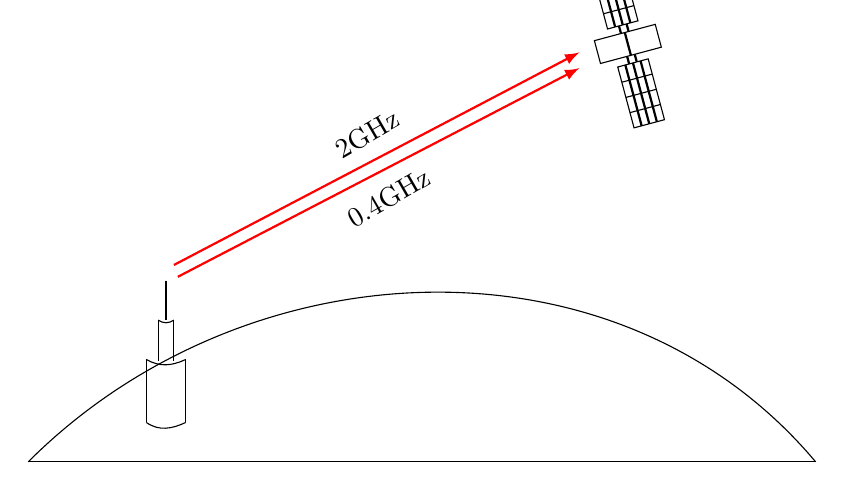
\begin{tikzpicture}
    \coordinate (lend) at (-5, 0);
    \coordinate (rend) at (5, 0);
    \draw (lend) to (rend);
    \draw (lend) to[out=45,in=-230] (rend);

    \coordinate (blb) at (-3.5, 0.5);
    \coordinate (brb) at (-3, 0.5);
    \draw (blb) to[out=-35,in=205] (brb);

    \coordinate (mlb) at (-3.5, 1.3);
    \coordinate (mrb) at (-3, 1.3);
    \draw (mlb) to[out=-30,in=205] (mrb);
    %\draw (mlb) to[out=35,in=-205] (mrb);
    \draw (blb) to (mlb);
    \draw (brb) to (mrb);
    
    \coordinate (tlb) at (-3.35, 1.8);
    \coordinate (trb) at (-3.15, 1.8);
    \draw (tlb) to[out=-35,in=215] (trb);
    \draw (tlb) to (-3.35, 1.28);
    \draw (trb) to (-3.15, 1.28);

    \coordinate (ulb) at (-3.26, 2.3);
    \coordinate (urb) at (-3.24, 2.3);
    \draw (ulb) to (-3.26, 1.8);
    \draw (urb) to (-3.24, 1.8);

    \rotatebox{15}{%
    \draw[] (3.5,4.6) rectangle (4.3,4.3);
    % Up panel
    \draw[thick] (3.9,4.3) to (3.9,4.6);
    \draw[thick] (3.85,4.6) to (3.85,4.7);
    \draw[thick] (3.95,4.6) to (3.95,4.7);
    \draw[] (3.7,5.5) rectangle (4.1,4.7);
    % grid
    \draw[thick] (3.8,4.7) to (3.8, 5.5); 
    \draw[thick] (3.9,4.7) to (3.9, 5.5); 
    \draw[thick] (4.0,4.7) to (4.0, 5.5); 
    \draw[] (3.7,4.9) to (4.1, 4.9);
    \draw[] (3.7,5.1) to (4.1, 5.1);
    \draw[] (3.7,5.3) to (4.1, 5.3);
    % Down panel
    \draw[thick] (3.85,4.3) to (3.85,4.2);
    \draw[thick] (3.95,4.3) to (3.95,4.2);
    \draw[] (3.7,3.4) rectangle (4.1,4.2);
    % grid
    \draw[thick] (3.8,3.4) to (3.8, 4.2); 
    \draw[thick] (3.9,3.4) to (3.9, 4.2); 
    \draw[thick] (4.0,3.4) to (4.0, 4.2); 
    \draw[] (3.7,3.6) to (4.1, 3.6);
    \draw[] (3.7,3.8) to (4.1, 3.8);
    \draw[] (3.7,4.0) to (4.1, 4.0);
    }
    
    \coordinate (satant1) at (2.0,  5.2);
    \coordinate (bcnant1) at (-3.15,2.5);
    \coordinate (satant2) at (2.0,  5.0);
    \coordinate (bcnant2) at (-3.10,2.35);
    \draw[thick,red,-latex] (bcnant1) -- node[above=1mm, align=center, black, rotate=30]{2GHz} (satant1);
    \draw[thick,red,-latex] (bcnant2) -- node[below=1mm, align=center, black, rotate=30]{0.4GHz} (satant2);

\end{tikzpicture}

  \caption{\gls{doris} System Description}
  \label{fig:doris-system-description}
\end{figure}

\gls{doris} (\cite{Barlier2005}) originated during the design phase of the US-French 
TOPEX/Poseidon mission (\cite{Fu1994}), 
and constitutes a Doppler up-link system, optimized for orbit determination (both 
in real-time and post-processed). Radio signals are generated from a ground-tracking 
network, and Doppler measurements are performed on-board the satellite. Since its 
initialization, the system's technology has greatly improved, and its applications 
have gradually and logically expanded from orbit determination to gravity-field 
determination, terrestrial reference frame maintenance and geodynamics. Since TOPEX/Poseidon, an 
ever-increasing number of \gls{leo} satellite missions are equipped with on-board 
\gls{doris} receivers. \autoref{fig:doris-constellations} depicts past, current and 
future \gls{doris}-equipped satellite missions.

\begin{figure}[h!]
  \centering
  \includegraphics[height=.4\textheight,keepaspectratio]{Constellation2021}
  \caption{DORIS-ecquiped satellites; image courtesy of \gls{ids}, source \url{https://ids-doris.org/doris-system/satellites.html}}
  \label{fig:doris-constellations}
\end{figure}

\gls{doris} is based on the accurate measurement of the Doppler shift of radio 
frequency signals transmitted from ground beacons and received on board the 
satellite(s) (\autoref{fig:doris-system-description}). Roughly every \SI{10}{\second}, 
the on-board receiver accurately measures 
the Doppler shift of radio-frequencies signals continuously transmitted from 
beacons at two frequencies: at \SI{2.03625}{\GHz} for precise Doppler measurement 
and at \SI{401.25}{\MHz} for correction of the propagation delay trough the 
ionosphere. The two channels are also used for time-tagging measurements and 
auxiliary data transmission (\cite{Auriol2010}).

\iffalse
\begin{description}
  \item[Atmospheric Studies] including troposphere () and ionosphere ()
  \item[Reference Frames] \cite{Willis2007}
  \item[Space Weather and Solar Activity] \cite{Willis2005}
  \item[Tectonics] \cite{}
\end{description}
\fi

\subsection{The DORIS Tracking Network}\label{ssec:doris-tracking-network}
The tracking network is a key factor in the success of the \gls{doris} system. 
\gls{ign} established and actively maintains this network, which currently (February
 2023) has 59 sites (\autoref{fig:doris-network}). It is global, dense 
and homogeneous, and thus unique among the different techniques that contribute to 
\gls{itrf}. Since its establishment, very few changes of sites and/or instrumentation 
have been performed, thus enforcing network stability. Furthermore, it is (spatially) 
dense and well distributed geographically (especially between the Northern and  
Southern hemispheres). This spatial balance along with several collocations with 
other space-geodetic techniques (\autoref{fig:doris-network-ties}), make the 
\gls{doris} system an integral part of reference frame maintenance (\cite{Moreaux2022}).

\begin{figure}[h]
  \centering
  \includegraphics[height=.4\textheight,keepaspectratio]{permanent_network_Nov2020}
  \caption{The \gls{doris} Network (as of Nov. 2020); image courtesy of \gls{ids}, source \url{https://ids-doris.org/doris-system/tracking-network/maps.html}}
  \label{fig:doris-network}
\end{figure}

The strengths and advantages of the \gls{doris} tracking network, can be summarized 
by (\cite{Soudarin2019})
\begin{description}
  \item[Centralized control and management] of the network deployment and evolution, 
    including site instrumentation.
  \item[Long operation time]; time-series of current stations span a 21 year period in average, 
    with a median of 26.4 years.
  \item[Homogeneous spatial distribution]; half of the stations are located on 
    islands or coastal areas and the network is well balanced between the 
    Northern and Southern hemispheres (\autoref{fig:doris-network}).
  \item[Large number of co-locations]; 48 stations are co-located with 
    other techniques (\gls{gnss}: 47, \gls{slr}: 10, \gls{vlbi}: 7), plus 28 are 
    co-located with tide gauges (\autoref{fig:doris-network-ties})
\end{description}

\begin{figure}[h]
  \centering
  \includegraphics[height=.4\textheight,keepaspectratio]{colocation_IERS_TG_Nov2020}
  \caption{\gls{doris} stations co-located with other space-geodetic techniques 
    and tide-gauges (as of Nov. 2020); image courtesy of \gls{ids}.}
  \label{fig:doris-network-ties}
\end{figure}

\subsection{The International DORIS Service}\label{ssec:ids}
The \gls{ids} was established in 2003, with the mission to (\cite{Soudarin2019})
\begin{itemize}
  \item provide support to research activities in geodesy and geophysics, based 
    on \gls{doris} data and derived products, and
  \item give access to data, products and documents related to the \gls{doris} system
\end{itemize}

The service is based on international cooperation on a volunteer basis and just like 
its geodetic counterparts (i.e. \gls{igs}, \gls{ilrs} and \gls{ivs} for \gls{gnss}, 
\gls{slr} and \gls{vlbi} respectively) plays a crucial role in the development of 
the technique and most importantly drives and facilitates its usage from the scientific 
community. Major products published by \gls{ids} include times series of the \gls{doris} 
tracking stations, along with their positions and velocities  and time series of 
geocenter motion and Earth orientation parameters. \gls{ids} also coordinates the 
technique's contribution to the \gls{itrf} (see e.g. \cite{Moreaux2022}).

\gls{ids}'s organization chart, includes a Governing Board and a Central Bureau.
The Analysis Centers process the \gls{doris} data available at the \gls{ids} Data 
Centers and generate products with the assistance of the Analysis Center Coordinator.
The \gls{ids} Combination Center provides regular combination of products of 
the Analysis Centers and is also in charge of the realization of the so-called 
DPOD (\gls{doris} extension to the current \gls{itrf} for \gls{pod}) 
which contains update mean positions and velocities of all the \gls{doris} stations. 
Last but not least, the \gls{ids} Combination Center produces the technique's 
contribution the \gls{itrf}.

\iffalse
\fi

  \section{DORIS Ground Segment}\label{sec:doris-ground-segment}

\subsection{Geometry of Ground Antennae}\label{ssec:antenae-geometry}
DORIS observations are referred to the electronic reference point (RP) of the 
antenna, the points where the DORIS observations  are  acquired.  As that 
electronic  point (\SI{2}{\GHz} center of phase for DORIS) is virtual and as 
for example it may change while using another type of antenna data referring 
to that electronic point are of no use for geophysical studies. So, 
observations must be referred to the conventional RP which is defined 
according to the geometry of the antenna. Therefore, one has also to account 
for the distance between the electronic RP and the conventional RP of the 
antenna (\cite{TOURAIN2016}). The ability to get accurate DORIS data relies 
for one part on the capability of providing accurate models to connect the 
electronic RP (or electronic phase center) and the conventional RP, as well 
as, phase center variations (\glspl{pcv}) as a function of the elevation angle 
and azimuth.

The type of antenna is identified by the 4\textsuperscript{th} character of 
the beacon mnemonic: letter ``A'' for the Alcatel type; letter ``B'' or letter 
``C'' for the Starec B or C type.  That is, in the DORIS RINEX field 
``STATION REFERENCE'', the last character of the second column (aka 
``4-character station code''), defines the ground beacon antenna type; 
example:

\begin{adjustbox}{max width=\linewidth , fbox=0.5pt}
\begin{BVerbatim}[commandchars=\\\{\}]
    51                                                      # OF STATIONS       
D01  BEM\textcolor{red}{B} BELGRANO                      66018S002  3   0    STATION REFERENCE   
D02  ADH\textcolor{red}{C} TERRE ADELIE                  91501S005  3   0    STATION REFERENCE   
D03  SYQ\textcolor{red}{B} SYOWA                         66006S005  3   0    STATION REFERENCE   
D04  CRQ\textcolor{red}{C} CROZET                        91301S004  4   0    STATION REFERENCE   
D05  DIO\textcolor{red}{B} DIONYSOS                      12602S012  3   0    STATION REFERENCE
\end{BVerbatim}
\end{adjustbox}

\begin{table}[h!]
    \centering
    \begin{tabular}{|c | c | c | c | c|}
        \hline
        \textbf{Zenith Distance} & \multicolumn{2}{c}{\textbf{ALCATEL (dBi)}} & \multicolumn{2}{c|}{\textbf{STAREC (dBi)}} \\
                        & \SI{401.25}{\mega\hertz} & \SI{2036.25}{\mega\hertz} &  \SI{401.25}{\mega\hertz} & \SI{2036.25}{\mega\hertz}\\
        \hline
        \ang{0}&3.2&2.1&3.5&0 \\
        \ang{10}&3.5&2.6&3.6&0.4\\
        \ang{20}&4&2&3.7&0.5\\
        \ang{30}&4.4&4&3.8&1.5\\
        \ang{40}&4.6&4.4&3.7&3.2\\
        \ang{50}&4.2&4.6&3.2&3.9\\
        \ang{60}&2.7&2.7&2.5&4\\
        \ang{70}&0.6&-0.1&1&3.2\\
        \ang{80}&-2.7&-3.3&-1.3&0.2\\
        \ang{90}&-6&-7&-4.2&-5.6\\
        \hline
    \end{tabular}
    \caption{DORIS ground antennae gains, \cite{DORISGSM}.}
    \label{table:antenna-gains}
\end{table}

\subsubsection{Phase Center Offsets}\label{sssec:doris-pco}
Depending on the antenna type, appropriate \gls{pco}s need to be applied to 
the observed quantities for the reduction of the observation vector to the 
Reference Point (from the respective ``virtual'' phase center) of the antenna. 
When a linear combination of the observed quantities is used, a respective 
\gls{pco} needs to be computed and applied. E.g., for the case of the 
ionospheric-free linear combination, the respective \gls{pco} is:
\begin{equation}
    \vec{r}_{2GHz,iono-free} = \frac{\vec{r}_{400MHz,2GHz}}{\gamma - 1}
\end{equation}

where $\vec{r}_{2GHz,iono-free}$ is the vector from the \SI{2}{\GHz} phase
center to the iono-free phase center and $\vec{r}_{400MHz,2GHz}$ is
the vector from the \SI{400}{MHz} to the \SI{2}{\GHz} phase center.

\begin{table}[h!]
    \centering
    \begin{tabular}{|c|c|c|}
        \hline
        \textbf{Antenna Type} & \textbf{ALCATEL} & \textbf{STAREC-B} \& \textbf{STAREC-C} \\
        \hline
        $\Delta h$ in \si{\mm} for \SI{2}{\GHz} & \SI{510}{\mm} & \SI{487}{\mm}\\
        $\Delta h$ in \si{\mm} for \SI{400}{\MHz} & \SI{335}{\mm} & \SI{0}{\mm}\\
        \hline
    \end{tabular}
    \caption{DORIS ground antennae Phase Center Offsets, \cite{DORISGSM}.}
    \label{table:antenna-pco}
\end{table}

\subsubsection{DORIS ALCATEL Antenna}\label{sssec:doris-alcatel}
\begin{figure}
\centering
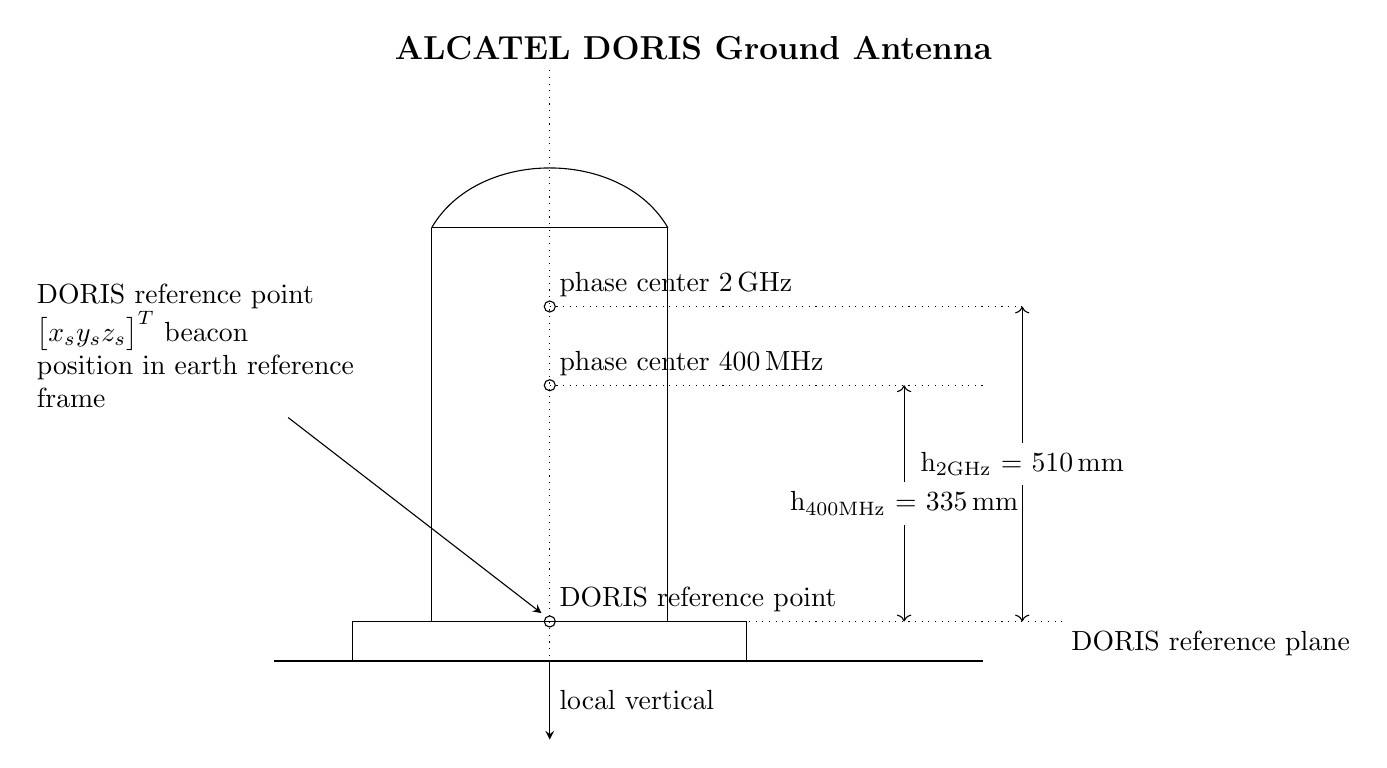
\begin{tikzpicture}
    \draw (2,-2) -- (2,-7); %% left vertical
    \coordinate (LT) at (2,-2);
    \draw (5,-2) -- (5,-7); %% right vertical
    \coordinate (RT) at (5,-2);
    \coordinate (L2PC) at (3.5, -4.0);
    \coordinate (L1PC) at (3.5, -3.0);
    \coordinate (BRP) at (3.5, -7.0);
    \draw (LT) to[out=60, in=120] (RT); %% dome
    \draw (LT) to (RT); %% top horizontal (under dome)
    \draw (1,-7) -- (6,-7); %% reference plain
    \draw (1, -7) -- (1, -7.5); %% left minor vertical
    \draw (6, -7) -- (6, -7.5); %% right minor vertical
    \draw [line width=0.25mm] (0,-7.5) -- (9,-7.5); %% ground
    \draw [-stealth] (3.5,-7.5) --node[anchor=west]{local vertical} (3.5, -8.5); %% local vertical to ground
    \draw [dotted] (3.5, 0) -- (3.5, -7.5); %% local vertical from dome
    
    \draw (L1PC) circle (2pt) node[anchor=south west]{phase center \SI{2}{\GHz}}; %% 2GHz pc
    \draw (L1PC) node[cross=3pt, rotate=0] {}; %% 2GHz cross
    \draw [dotted] (L1PC) -- (9.5, -3.0); %% horizontal from 2GHz PC
    \path (9.5, -7.0) -- node[](hl1){h\textsubscript{2GHz} = \SI{510}{\mm}} (9.5, -3.0);
    \draw [<-] (9.5, -7.0)--(hl1); \draw [->] (hl1)--(9.5, -3.0);
    
    \draw (L2PC) circle (2pt) node[anchor=south west]{phase center \SI{400}{\MHz}}; %% 400 MHz pc
    \draw (L2PC) node[cross=3pt, rotate=0] {}; %% 400MHz cross
    \draw [dotted] (L2PC) -- (9, -4.0); %% horizontal from 400MHz PC
    \path (8, -7.0) -- node[](hl2){h\textsubscript{400MHz} = \SI{335}{\mm}} (8, -4.0);
    \draw [<-] (8, -7.0)--(hl2); \draw[->] (hl2)--(8, -4.0);
    
    \draw (BRP) circle (2pt) node[anchor=south west]{DORIS reference point}; %% reference point
    \draw (BRP) node[cross=3pt, rotate=0] {}; %% RP cross
    \draw [dotted] (BRP) -- (10, -7.0); %% horizontal from RP
    \draw (10, -7) node[anchor=north west]{DORIS reference plane};
    
    \node[rectangle, align=left] (rptext) at (-1,-3.5) {DORIS reference point \\ \(\begin{bmatrix} x_s y_s z_s \end{bmatrix}^{T} \) beacon \\position in earth reference \\frame};
    \draw [-stealth] (rptext) to ($(BRP)-(3pt,-3pt)$);
    \node[above,font=\large\bfseries] at (current bounding box.north) {ALCATEL DORIS Ground Antenna};
\end{tikzpicture}

\caption{Geometry of Alcatel DORIS Ground Antenna/Beacon}
\label{fig:alcatel-antenna}
\end{figure}


\subsubsection{DORIS STAREC Antenna}\label{sssec:doris-starec}
STAREC antennae B and C are identical in terms of design and specification, the
difference is about the error budget in phase center position. For STAREC-C,
manufacturing process and error budget have been improved \cite{DORISGSM}.

According to \cite{TOURAIN2016}, in order to check the consistency of the theoretical 
characteristics of this type of antennae, a measurement campaign was performedby 
the \gls{cnes} at the \gls{catr}. The \gls{catr} is a dedicated facility 
consisting of an anechoic chamber equipped with several specific devices 
allowing significant measurement for satellite characterization.

As a result of the campaign, a phase law was established by averaging the 
estimated phase law values obtained during the \gls{catr} characterization. 
The resulting couple phase center position–phase law correction was provided 
to the DORIS users through a text file in \gls{antex} (\cite{ANTEXv14}) format, 
made available by \gls{ids} at 
\url{ftp://ftp.ids-doris.org/pub/ids/stations/doris_phase_law_antex_starec.txt}.

STAREC antennae B and C are identical in terms of design and specification, the
difference is about the error budget in phase center position. For STAREC C,
manufacturing process and error budget have been improved (\cite{DORISGSM}).

\begin{figure}
\centering
\tikzset{cross/.style={cross out, draw=red, minimum size=2*(#1-\pgflinewidth), inner sep=0pt, outer sep=0pt},
%default radius will be 1pt. 
cross/.default={1pt}}

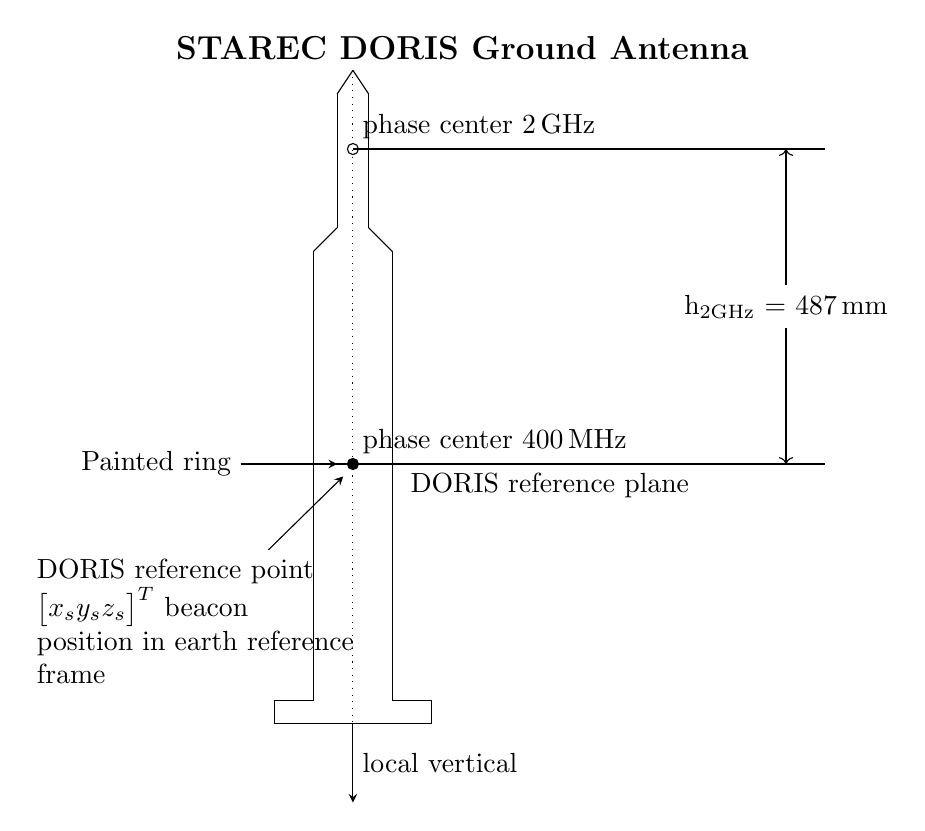
\begin{tikzpicture}
    \coordinate (top) at (4,-1);
    \coordinate (tl) at (3.8, -1.3);
    \coordinate (tr) at (4.2, -1.3);
    \coordinate (blt) at (3.8, -3.0);
    \coordinate (brt) at (4.2, -3.0);
    \coordinate (blb) at (3.5, -3.3);
    \coordinate (brb) at (4.5, -3.3);
    \draw (top) to (tl);
    \draw (tl) to (blt);
    \draw (blt) to (blb);
    \draw (top) to (tr);
    \draw (tr) to (brt);
    \draw (brt) to (brb);
    \draw (blb) to (3.5, -9);
    \draw (brb) to (4.5, -9);
    \draw (3.5, -9) to (3.0, -9);
    \draw (3.0, -9) to (3.0, -9.3);
    \draw (4.5, -9) to (5.0, -9);
    \draw (5.0, -9) to (5.0, -9.3);
    \draw (3.0, -9.3) to (5.0, -9.3);

    \draw [dotted] (top) -- (4.0, -9.3); %% local vertical from top
    \draw [-stealth] (4.0, -9.3) -- node[anchor=west]{local vertical} (4.0, -10.3); %% local vertical arrow

    \coordinate (l1pc) at (4, -2.0);
    \draw (l1pc) circle (2pt) node[anchor=south west]{phase center \SI{2}{\GHz}}; %% 2GHz pc
    \draw (l1pc) node[cross=3pt, rotate=0] {}; %% 2GHz cross
    \draw (l1pc) to (10, -2.0);
    
    \coordinate (l2pc) at (4, -6.0);
    \draw [fill=black] (l2pc) circle (2pt) node[anchor=south west]{phase center \SI{400}{\MHz}}; %% 400MHz pc
    \draw (l2pc) node[cross=3pt, rotate=0] {}; %% 400MHz cross
    \draw ($(l2pc)-(1.0,0.0)$) -- node[below]{DORIS reference plane} (10, -6.0);
    \node (prt) at ($(l2pc)-(2.5,0.0)$) {Painted ring}; 
    \draw [-stealth] (prt) to ($(l2pc)-(0.2,0.0)$);

    \path ($(l1pc)+(5.5, 0.0)$) -- node[](h2g){h\textsubscript{2GHz} = \SI{487}{\mm}} ($(l2pc)+(5.5, 0.0)$);
    \draw [<-] ($(l1pc)+(5.5, 0.0)$) -- (h2g); 
    \draw [->] (h2g) -- ($(l2pc)+(5.5, 0.0)$);

    \node[rectangle, align=left] (rptext) at ($(l2pc)-(2.0,2.0)$) {DORIS reference point \\ \(\begin{bmatrix} x_s y_s z_s \end{bmatrix}^{T} \) beacon \\position in earth reference \\frame};
    \draw [-stealth] (rptext) to ($(l2pc)-(3.5pt,4.5pt)$);

    \node[above,font=\large\bfseries] at (current bounding box.north) {STAREC DORIS Ground Antenna};
\end{tikzpicture}

\caption{Geometry of Alcatel STAREC Ground Antenna/Beacon}
\label{fig:starec-antenna}
\end{figure}

\subsubsection{Phase Law}\label{doris-phase-law}

\begin{figure}
\centering
\begin{tikzpicture}
\pgfplotstableread{tikz/phase_law.dat}{\table}
\begin{groupplot}[
  group style={
        group name= phase-law-plots,
        group size=1 by 2,
        xlabels at=edge bottom,
        xticklabels at=edge bottom,
        vertical sep=8pt,
    },
  %title={\texttt{patch type=quadratic spline}},
  xmin=0, xmax=90,
  ymin=-5, ymax=25,
  xtick distance = 5,
  ytick distance = 5,
  grid = both,
  minor tick num = 1,
  major grid style = {lightgray},
  minor grid style = {lightgray!25},
  width = \textwidth,
  height = 0.4\textwidth,
  xlabel = {Zenith angle ($^{\circ}$)},
]
\nextgroupplot[]
\addlegendimage{empty legend};
%\addplot[blue, mark = *] table [x = {Zenith}, y = {Alcatel_1}] {\table};
\addplot[mark=o,mark size=0.6pt] table [x = {Zenith}, y = {Alcatel_1}] {\table};
\addlegendentry{\texttt{Alcatel Antenna}}[15 pt];
\coordinate (top) at (rel axis cs:0,1);% coordinate at top of the first plot

\nextgroupplot[]
\addlegendimage{empty legend};
\addplot[mark = *,mark size=0.6pt] table [x = {Zenith}, y = {Starec_1}] {\table};
\addlegendentry{\texttt{Starec Antenna}}[15 pt];
\coordinate (bot) at (rel axis cs:0,0);% coordinate at bottom of the last plot

\end{groupplot}

\path (top-|current bounding box.west)-- node[anchor=south,rotate=90] 
  {Phase Correction for 2GHz ($mm$)} (bot-|current bounding box.west);

\path (top-|current bounding box.west) --
  node[anchor=south]{\textbf{DORIS Antennae Phase Law}} 
  (top-|current bounding box.east);
%\node (title) at ($(group c1r1.center)!0.5!(group c2r1.center)+(0,2cm)$) 
%  {DORIS Antenae Phase Law};
\end{tikzpicture}

\caption{DORIS Antennae Phase Law}
\label{fig:doris-antennae-phase-law}
\end{figure}

  \section{DORIS RINEX}\label{sec:doris-rinex}

\subsection{General Format  Description}
The DORIS RINEX format consists of one ASCII file containing both space based 
and meteorological data collected at DORIS stations and relayed by satellites.

DORIS RINEX format bears close resemblance\footnote{The format specifications are 
actually close to identical.} to the GNSS RINEX Version 3 (\cite{RINEX305}).
Data files consist of a header section and a data section. The first contains 
global information for the entire file, while the latter contains the actual 
observations and a date tag, keeping strict chronological order.

DORIS is basically running on its own proper time which is constantly linked 
to \gls{tai}. Time tags are given in instrument time, clock offsets are given 
between instrument time and \gls{tai}.

Observation types recorded in the DORIS RINEX files are the given in table

\begin{table}[h!]
\centering
\begin{tabular}{|c c c|}
\hline
Descriptor & Observation Type & Units \\
\hline
\texttt{L} & carrier phase observation & cycles \\
\texttt{C} & pseudo-range observation & \si{\metre}\\
\texttt{W} & power level received at each frequency & \si{\dBm} \\
\texttt{F} & relative frequency offset of the receiver’s oscillator $\frac{f-f_0}{f_0}$ & $10^{-11}$ \\
\texttt{P} & ground pressure at the station & 100 \si{\pascal} (\si{\milli\bar}) \\
\texttt{T} & ground temperature at the station & \si{\degreeCelsius} \\
\texttt{H} & ground humidity at the station & \si{\percent} \\
\hline
\end{tabular}
\caption{DORIS RINEX observation types}
\label{table:doris-rinex-observation-types}
\end{table}

\subsection{Receiver Clock Offsets}

DORIS RINEX contain a ``receiver clock offset'' \(\tau_{r_{offset}}\) (as an 
optional field) at the header record of every epoch. E.g. the line
\begin{verbatim}
    ...
    > 2020 01 01 00 00 35.099949800  0  1       -3.248177132 0
    ...
\end{verbatim}
records a receiver clock offset of \SI{35.099949800}{\second} followed by the 
receiver clock offset flag, which in this case is \num{0}. In such record 
lines, the date (given as YYYY MM DD HH MM SS.) is given in the on-board time 
scale (aka proper time of the receiver) and the conversion to the \gls{tai} 
time scale is obtained by adding the receiver clock offset.

\textit{Depending on the version of the RINEX file, this offset can have been either 
computed by the DORIS-DIODE navigator, or through a post-fit processing using PANDOR. 
In the first case, the file ends with ``.001'' whereas in the second with ``.010''. 
More information on the computation of (\(\tau_{r_{offset}}\) are provided in 
\cite{lemoine-2016}.}

\subsection{Types of DORIS measurements}
\label{ssec:types-of-doris-measurements}

\subsubsection{Relative Frequency Offset}
\label{sssec:relative-frequency-offset}

DORIS RINEX files (usually) contain a measurement type labeled ``F'' (should be 
recorded in the field \verb|SYS/#/OBS TYPES| at the RINEX header). This measurement 
type is provided for every epoch and is a measure of the relative frequency 
offset of the receiver's oscillator (aka \(\frac{f-f_0}{f_0}\) \num{10e-11}).
Example (rinex header):

\begin{adjustbox}{max width=\linewidth , fbox=0.5pt}
\begin{BVerbatim}
        0.9768        0.0001        0.0011                  CENTER OF MASS: XYZ
D   10  L1  L2  C1  C2  W1  W2   F   P   T   H              SYS / # / OBS TYPES
  2018    01    01    00    00   28.8526816     DOR         TIME OF FIRST OBS
...
                                                            END OF HEADER
> 2018 01 01 00 00 32.589951370  0  3       -3.737269708 0
D01  -2104936.480    -1241282.301   131837622.17412 131837685.14912      -124.650 7
         -114.150 7      5643.911        1025.000 1         6.000 1        85.000 1
D02  -1063469.796    -1862572.573   136575183.93813 136575216.89713      -118.350 7
         -109.250 7      5643.911        1014.000 0       -18.800 0        73.000 0
D03   -826480.354    -2642364.157   148404267.53014 148404098.13114      -115.200 7
         -104.700 7      5643.911         934.000 0       -21.500 0        72.000 0
...                                                            
\end{BVerbatim}
\end{adjustbox}

  \section{\gls{doris} Observation Equation}\label{sec:doris-observation-equation}

\subsection{Theoretical Model of Doppler Observations}\label{ssec:doris-obs-theory}
A detailed derivation of the Doppler observation equation, as implemented by means of the 
\gls{doris} system, can be found in \cite{Lemoine2016}, including a thorough theoretical 
discussion. A brief overview is given here, with focus on the measurement model 
implementation.

To gain a clear view on the model of the measurements, a rigorous distinction of 
events must be made; four different events can be identified:
\begin{description}
    \item[beginning of emission] of the 1\textsubscript{st} cycle by the emitter, 
    \(\tau_{e_1}\) in the proper time scale of the emitter and \(t_1\) in the coordinate 
    time
    
    \item[beginning of reception] of the 1\textsubscript{st} cycle by the receiver, 
    \(\tau_{r_1'}\) in the proper time scale of the receiver and 
    \(t_{1'}\) in the coordinate time

    \item[end of emission] of the N\textsubscript{th} cycle by the emitter, 
    \(\tau_{e_2}\) in the proper time scale of the emitter and \(t_2\) in the coordinate 
    time
    
    \item[end of reception] of the N\textsubscript{th} cycle by the receiver, 
    \(\tau_{r_2'}\) in the proper time scale of the receiver and 
    \(t_{2'}\) in the coordinate time
\end{description}

During the proper time interval $\Delta\tau_{r} = \tau_{r2'} - \tau_{r1'}$, 
the receiver has received the $N_e$ cycles sent by the emitter, with $N_e = f_e \Delta\tau_e$, 
$f_e$ being the proper frequency of the emitter. The receiver is also equipped with
an oscillator and during the proper time interval $\Delta\tau_{r}$ has generated 
a number $N_r = f_r \Delta\tau_r$ of cycles, $f_r$ being the proper frequency of the 
receiver.

The Doppler measurement is the count, by the receiver electronics, of the number 
of cycles of difference between \(N_e\) and \(N_r\):
\begin{equation}
    \begin{split}
    N_{DOP} & = N_e - N_r\\
            & = f_e \Delta\tau_e - f_r \Delta\tau_r
    \end{split}
\end{equation}

\emph{In the RINEX files, this Doppler count is the difference between two phase measurements 
done at different time tags in the proper time-scale of the receiver.}

After a series of assumptions and simplifications, theoretical formula for the 
Doppler count can be written as (\cite{Lemoine2016}):
\begin{equation}
    \begin{split}
        \frac{c}{f_e \Delta\tau_r} N_{DOP} & \approx c \frac{f_e - f_r}{f_e} \\
        & - (1 - \frac{U_e}{c^2} - \frac{{V_e}^2}{2 c^2}) \frac{\rho_2 - \rho_1}{\Delta\tau_r}\\
        & + \frac{1}{c} (U_r - U_e + \frac{{V_r}^2 - {V_e}^2}{2}) \\
        & + \frac{2 \mu}{c^2 \Delta\tau_r} [\ln{(\frac{R_1 + R_{1'} + \rho_1}{R_1 + R_{1'} - \rho_1})} - \ln{(\frac{R_2 + R_{2'} + \rho_2}{R_2 + R_{2'} - \rho_2})}]
    \end{split}
\end{equation}
where
\begin{description}
  \item $c$ is the velocity of light in vacuum,
  \item $f_e$ and $f_r$ are the emitter's and receiver's proper frequencies,
  \item $U_e$ and $U_r$ are the gravitational potential at the emitter and receiver,
  \item $V_e$ and $V_r$ is the velocity of the clock at the emitter and receiver 
    (in the coordinate reference frame),
  \item $\rho _i$ is the curvlinear trajectory (of the photon(s)) at the event $i$,
  \item $R_i$ is the geometric distance between the beacon and the satellite at event $i$
\end{description}

The above equation can be conveniently split into two parts, one containing the ``measured'' 
quantities and one with the ``theoretical'' terms, as 
\begin{subequations}\label{eq:lem12}
  \begin{align}
    v_{measured} & = \frac{c}{f_e} (f_e - f_r -
     \frac{N_{DOP}}{\Delta\tau_r}) + \Delta u_{REL} \label{eq:lem12a} \\
    v_{theo}     &= \frac{\rho_2 - \rho_1}{\Delta\tau_r} (1- \frac{U_e}{c^2} - 
      \frac{{V_e}^2}{2 c^2}) \label{eq:lem12b}
  \end{align}
\end{subequations}
with
\begin{equation}
    \begin{split}
        \Delta v_{REL} &= \frac{1}{c} (U_r - U_e + \frac{{V_r}^2 - {V_e}^2}{2}) \\
        & + \frac{2 \mu}{c^2 \Delta\tau_r} [\ln{(\frac{R_1 + R_{1'} + \rho_1}{R_1 + R_{1'} - \rho_1})} - \ln{(\frac{R_2 + R_{2'} + \rho_2}{R_2 + R_{2'} - \rho_2})}]
    \end{split}
\end{equation}

It is well known that signals transmitted through the Earth's atmosphere are 
affected by it (delayed); let $\Delta v_{IONO}$ and $\Delta v_{TROPO}$, be the 
propagation corrections of the radio electric signal through the ionosphere and 
troposphere respectively. 

Additionally, in the actual case (measurements), the nominal frequencies $f_e$ and $f_r$ 
are not the ``true'' ones; hence, a relative correction needs to be applied e.g. for the 
emitter $f_{e_T} = f_{e_N} (1 + \frac{\Delta f_e}{f_{e_N}})$, where the subscript $T$ 
denotes the ``True'' frequency and $N$ the nominal one. Thus in \autoref{eq:lem12} the 
terms $f_e$ and $f_r$ need to be substituted by $f_{e_T}$ and $f_{r_T}$ respectively.

$\Delta v_{IONO}$ and $\Delta v_{REL}$, which do not involve adjusted parameters, can be placed 
on the ``measured'' part of \autoref{eq:lem12} and $\Delta v_{TROPO}$ and $\frac{\Delta f_e}{f_{e_N}}$ 
on the ``theoretical'' part. Furthermore, since $\Delta f_e / f_{e_N} \ll 1$ all  
terms including $\Delta f_e / f^2_{e_N}$ and $\left(\Delta f_e / f_{e_N}\right)^2$ 
can be safely neglected and \autoref{eq:lem12} can be rewritten as:
\begin{subequations}\label{eq:lem13}
    \begin{align}
        v_{measured} & = \frac{c}{f_{e_N}} (f_{e_N} - f_{r_T} -
          \frac{N_{DOP}}{\Delta\tau_r}) + \Delta u_{REL} + 
          \Delta u_{IONO} \label{eq:lem13a} \\
        v_{theo} &= \frac{\rho_2 - \rho_1}{\Delta\tau_r} 
          (1- \frac{U_e}{c^2} - \frac{{V_e}^2}{2 c^2}) + 
          \Delta u_{TROPO} - \frac{c(\frac{N_{DOP}}{\Delta\tau_r} + 
          f_{r_T})}{f_{e_N}} \frac{\Delta f_e}{f_{e_N}} \label{eq:lem13b}
    \end{align}
\end{subequations}
where 
\begin{description}
    \item[$v_{measured}$] is the measured relative velocity between the emitter and 
    the receiver between the events 1' and 2', based on the Doppler count $N_{DOP}$, 
    corrected for the ionospheric and relativistic effects.

    \item[$v_{theo}$] is the theoretical (computed) emitter/receiver relative velocity 
    between the events 1' and 2', corrected for the tropospheric effect and for a solved-for 
    frequency bias $\frac{\Delta f_e}{f_{e_N}}$ of the emitter. 
    $f_{r_T} = f_{r_N} (1 + \frac{\Delta f_r}{f_{r_N}})$ 
    is an estimate of the proper frequency of the receiver.

    \item[$\Delta v_{REL} = \Delta v_{{REL}_c} + \Delta v_{{REL}_r}$] is the relativistic 
    correction, composed of two parts: the clock correction $\Delta v_{{REL}_c}$ and the 
    travel correction $\Delta v_{{REL}_r}$
    \begin{subequations}\label{eq:lem14}
        \begin{align}
            \Delta v_{{REL}_c} & = \frac{1}{c} 
              (U_r - U_e + \frac{{V_r}^2 - {V_e}^2}{2}) \label{eq:lem14a}\\
            \Delta v_{{REL}_r} & = \frac{2 \mu}{c^2 \Delta\tau_r} \left[ 
              \ln{(\frac{R_1 + R_{1'} + \rho_1}{R_1 + R_{1'} - \rho_1})} - 
              \ln{(\frac{R_2 + R_{2'} + \rho_2}{R_2 + R_{2'} - \rho_2})} \right] \label{eq:lem14b}
        \end{align}
    \end{subequations}
\end{description}

Note that \autoref{eq:lem13a} and \autoref{eq:lem13b} can be further simplified 
to \autoref{eq:lem17a} and \autoref{eq:lem17b} respectively, by 
omitting small terms (\autoref{sssec:small-terms}).

\subsection{Computational Aspects}\label{ssec:doris-computational-aspects}

\subsubsection{Small Terms}\label{sssec:small-terms}
In \autoref{eq:lem13a} and \autoref{eq:lem13a}, the smallest terms are $-U_e / c^2 - {V_e}^2 / 2 c^2$ and 
$\Delta v_{{REL}_T}$; in the case of \gls{doris} they amount to \num{11.} and 
\num{6.} \SI{10e-6}{\meter\per\second} respectively (\cite{Lemoine2016}). 
Furthermore, since the emitters are located on the ground, the term 
$-U_e / c^2 - {V_e}^2 / 2 c^2$ is constant per station. This small 
relativistic offset is absorbed by the adjustment of $\Delta f_e / f_{e_N}$. 
So it is possibly to further simplify \autoref{eq:lem13a} and \autoref{eq:lem13b} 
to:
\begin{subequations}\label{eq:lem17}
    \begin{align}
        v_{measured} & = \frac{c}{f_{e_N}} (f_{e_N} - f_{r_T} -
          \frac{N_{DOP}}{\Delta\tau_r}) + 
          \Delta u_{{REL}_C} + \Delta u_{IONO} \label{eq:lem17a}\\
        v_{theo} &= \frac{\rho_2 - \rho_1}{\Delta\tau_r} + \Delta u_{TROPO} - 
          \frac{c(\frac{N_{DOP}}{\Delta\tau_r} + f_{r_T})}{f_{e_N}} 
          \frac{\Delta f_e}{f_{e_N}} \label{eq:lem17b}
    \end{align}
\end{subequations}

\subsubsection{Correction of Aberration}\label{sssec:doris-aberration}
In \autoref{eq:lem13b} (or \autoref{eq:lem17b}), $\rho _i$ is the geometrical distance 
between the emitter at time $t_i$ and the receiver at time $t_{i'}$ (with $i=1,2$). 
The measurements are made by the receiver electronics, hence the instance $t_i$ is 
actually unknown. In order to compute accurately $t_i$ and thus the position of 
the emitter at this instant in time, a \emph{correction of aberration} (\cite{Lemoine2016}) 
has to be performed. This correction can be evaluated in an iterative manner: an 
approximate value of the emitter-receiver distance $\rho ^{*} _i$ is first computed, 
by evaluating the position of the beacon at time $t_{i'}$. Subsequently, $t_i$ can be 
found via $t_i = t_{i'} - \rho ^{*} _i / c$. In practice, one iteration is enough.

\subsubsection{Geopotential}\label{sssec:doris-geopotential}
For a station on the geoid, the potential at the level of the station is the sum 
of the gravitational potential and the centrifugal potential due to the Earth's 
rotation: $U_{GEO} = U_e + \frac{{V_e}^2}{2}$, which is a constant. For a station 
not located on the geoid, the quantity $U_e + \frac{{V_e}^2}{2}$ will only depend 
on the height of the beacon above the geoid.

For the computation of the gravitational potential for \gls{leo} satellites, 
the potential $U_r$ cannot be restricted to the central term only ($GM_{\Earth} / r$) and
the Earth's oblateness ($J_2$) effect should also be considered (\cite{Larson2007}). 
Hence, the equation used for computing the potential for a given satellite, reads 
(\cite{Lemoine2016})
\begin{equation}\label{eq:lem18}
  U_r = 
    -\frac{GM_{\Earth}}{r} \left( 
      1 - 
      \left( \frac{R_{\Earth}}{r} \right) ^2 
      J_2 \frac{3 sin^2(\phi) - 1}{2} 
    \right)
\end{equation}
or in Cartesian coordinates (\cite{Larson2007})
\begin{equation}
  U_r = -\frac{GM_{\Earth}}{r} \left( 1- \left(\frac{R_{\Earth}}{r}\right)^2 
    J_2 \frac{3 z^2 - r^2}{2r^2} \right)
\end{equation}
with $R_{\Earth}$ the equatorial radius of the earth, $r$ radial 
distance of the satellite (to the Earth's center), $\phi$ latitude of the 
satellite and $J_2 = 1.0826359 \dot 10^{-3}$ in the zero-tide system (\cite{iers2010}).

\iffalse
\subsubsection{True Proper Frequency of the Receiver}\label{sssec:true-proprtfrequency-of-the-receiver}
For the term $f_{r_T}$ that appears in \autoref{eq:lem13a} and \autoref{eq:lem13b}, we need an estimate of 
$\Delta f_{r} / f_{r_N}$. This estimate can be obtained in one of the following ways 
\cite{Lemoine2016}:
\begin{enumerate}
    \item Via the field ``F'' recorded for every single measurement in the \gls{doris} 
      RINEX file (see \autoref{ssec:relative-frequency-offset}); not that this estimation 
      is not very smooth, as noticed by \cite{Gao2015} and it is advisable, before 
      using it in \autoref{eq:lem13}, to perform a linear (or polynomial) regression of 
      these estimates over one or a few days.
    \item It can be obtained from a polynomial regression over the frequency 
      offsets estimated during the passes over the master beacons
    \item It can be estimated as a by-product during a re-computation of the 
      ``timetagging'' polynomial (see \cite{Mercier2010})
\end{enumerate}
\fi

\subsubsection{Nominal Receiver and Emitter Frequencies}\label{ssec:nominal-frequencies}
In the observation equation model \autoref{eq:lem13a} and \autoref{eq:lem13b}, a distinction is made between 
\emph{nominal} and \emph{true} receiver/emitter frequencies, to account for the 
fact that in ``real world'' these two are not actually equal.

\paragraph{Emitter (Beacon) Nominal Frequencies, $f_{e_N}$}\label{par:beacon-nominal-frequencies}
RINEX file headers, contain values of the \emph{station frequency shift 
factor} $k$ for each of the beacons involved (\cite{DORISRNX3}, Sec. 6.16). 
These are used to compute the ``nominal'' frequencies of the beacon/emitter 
(usually, this shift factor is just $0$, but it can be an integer 
$k \neq 0$). The frequencies are computed as (\cite{DORISRNX3}, Sec. 6.16):
\begin{equation}
  \begin{aligned}
    L_{2GHz}   &= 543 \cdot F_0 \left( \frac{3}{4} + \frac{87\cdot k}{5 \cdot 2^{26}} \right) \\
    L_{400MHz} &= 107 \cdot F_0 \left( \frac{3}{4} + \frac{87\cdot k}{5 \cdot 2^{26}} \right) 
    \label{eq:nominal-freq}
  \end{aligned}
\end{equation}
where $F_0 = 5e6 \text{ Hz}$ the \gls{uso} frequency. These value, are the ones 
labelled as $f_{e_N}$ in \autoref{eq:lem13a} and \autoref{eq:lem13b}.

The \emph{true proper frequency} of the emitter $f_{e_T}$, can be computed (if needed) 
from:
\begin{equation}
  f_{e_T} = f_{e_N} \cdot \left( 1 + \frac{\Delta f_e}{f_{e_N}} \right)
\end{equation}
but the quantity $\Delta f_e / f_{e_N}$ is not known a-priori and has to be 
estimated during the processing.

The quantity $\Delta f_e / f_{e_N}$  can be estimated either as a constant term (bias), 
or using a linear model (bias ad drift). In the latter case (followed in this Thesis), 
the model can be written as:
\begin{equation}
  \frac{\Delta f_e}{f_{e_N}}\at{\tau=\tau _i} = \alpha + \beta \cdot \delta \tau
\end{equation}
For the estimation, the partials of the observation equation \autoref{eq:lem13b} are needed, 
with respect to $\alpha$ and $\beta$ parameters, which are:
\begin{equation}
  \begin{aligned}
  \frac{\partial v_{theo}}{\partial \alpha} &= 
    \frac{c(\frac{N_{DOP}}{\Delta\tau_r} + f_{r_T})}{f_{e_N}} \\
  \frac{\partial v_{theo}}{\partial \beta} &= 
    \frac{c(\frac{N_{DOP}}{\Delta\tau_r} + f_{r_T})}{f_{e_N}} \cdot \delta \tau
  \end{aligned}
\end{equation}

\paragraph{Receiver True Proper Frequency $f_{r_T}$}\label{par:receiver-true-proper-frequency}
In \autoref{eq:lem13a} and \autoref{eq:lem13b}, $f_{r_T}$ is the \emph{true proper frequency of 
the receiver}, computed as
\begin{equation}\label{eq:frt-gen}
  f_{r_T} = f_{r_N} \cdot \left( 1 + \frac{\Delta f_r}{f_{r_N}} \right)
\end{equation}
where $f_{r_N}$ is the ``nominal'' frequency value. The value of the quantity 
$\Delta f_r / f_{r_N}$, called the \emph{relative frequency offset} of the receiver,
can be extracted from the RINEX file, estimated or computed, in one of the following 
ways (\cite{Lemoine2016})
\begin{enumerate}
    \item Via the field ``F'' recorded for every single measurement in the \gls{doris} 
      RINEX file (see \autoref{sec:doris-rinex}); not that this estimation 
      is not very smooth, as noticed by \cite{Gao2015} and it is advisable, before 
      using it in \autoref{eq:lem13}, to perform a linear (or polynomial) regression of 
      these estimates over one or a few days.
    \item Obtained from a polynomial regression over the frequency 
      offsets estimated during the passes over the master beacons
    \item Estimated as a by-product during a re-computation of the 
      ``timetagging'' polynomial (see \cite{Mercier2010})
\end{enumerate}

Relative frequency offset values, $\frac{\Delta f_r}{f_{r_N}}$, are reported in the RINEX files for each epoch 
(under the observable tagged \texttt{F}). Note that these values are scaled to 
$10^{-11}$ (\cite{DORISRNX3}, Sec. 6.11), so that for a given epoch $t_i$, the 
true frequency is
\begin{equation}\label{eq:frt-rinex}
  f_{r_T}\at{t=t_i} = f_{r_N} \cdot \left( 1 + F_{t_i} \cdot 10^{-11} \right)
\end{equation}
where $F_{t_i}$ is the relative frequency offset value recovered from the RINEX 
file.

\subsection{Ionospheric Correction}\label{ssec:iono-correction}
The basic observation equation \autoref{eq:lem13a} and \autoref{eq:lem13b}, is formed for the \SI{2}{\GHz} 
carrier. For each measurement, the ionospheric path delay has to be corrected for, 
by computing a correction (in cycles) as (\cite{Lemoine2016}, Sec. 2.5.7):
\begin{equation}
  \delta_{ION} [\SI{2}{\GHz}\text{ cycles}] = 
    \frac{L_{\SI{2}{\GHz}} - \sqrt{\gamma} \cdot L_{\SI{400}{\MHz}}}{\gamma - 1}
  \label{eq:iono-delay-cycles}
\end{equation}
which is added to the \SI{2}{\GHz} measurement at time $t=t_i$ (obtained by the 
RINEX file). Thus, the corrected observation is:
\begin{equation}\label{eq:l2if}
  L_{\SI{2}{\GHz},IF} [\SI{2}{\GHz}\text{ cycles}] = 
    L_{\SI{2}{\GHz}} + \delta_{ION}
\end{equation}

Note that after applying \autoref{eq:l2if}, the measurement is referred to the ``Iono-Free'' 
geometrical endpoints of the signal path (and not the \SI{2}{\GHz} endpoints). 
This means that the respective {phase center corrections (i.e. \gls{pco} and \gls{pcv})
both at the satellite and at the beacon have to be applied.

  \section{Implementation of the \gls{doris} Observation Equation}\label{sec:doris-observation-equation-implementation}
The observation equation formed to process the \gls{doris} data, is based on 
\autoref{eq:lem17}. Consequently, two parts are computed, $v_{measured}$ which 
represents the ``observed'' or ``measured'' relative velocity between the receiver 
and the transmitter, and $v_{theo}$ which is the ``computed'' or ``theoretical'' 
counterpart. In this way, during the processing phase, all quantities that do not 
need adjustment can be placed on the ``measured'' side of the equation (\cite{Lemoine2016}).

A short discussion follows, describing the implementation of the \gls{doris} 
observation equation in the software designed for this Thesis.

\subsection{Coordinate and Proper Time}\label{ssec:coordinate-proper-time}
\gls{tai} is used as coordinate time; to transform RINEX observation time (given in 
proper time $\tau$) to coordinate time $t$, we use the \emph{receiver clock 
offset} values, extracted from the RINEX file (one value per observation block).

Hence, if an observation block is taged at proper time $\tau _i$ at the RINEX 
file, and the receiver clock offset for this block is $\Delta \tau _i$ (again from 
RINEX), then the coordinate time of the event in \gls{tai} is:
\begin{equation}
  t^{TAI}_i = \tau _i + \Delta \tau _i
\end{equation}

According to \cite{Lemoine2016} however, there is no need to make a time conversion 
for the time interval of the Doppler count, i.e. the term $\Delta \tau _r$ in 
\autoref{eq:lem17}, due to the time-tagging method used in \gls{doris} RINEX.

\subsection{Receiver Emitter Geometric Distance}
The geometric distances between the emitter and the receiver, $\rho _1$ and $\rho _2$, 
when computed, are corrected for the aberration effect, i.e. the slight displacement of 
the emitter due to Earth's rotation between signal emission and signal reception at
the receiver. The algorithm for this correction is described in \autoref{sssec:doris-aberration}.

\subsection{Relativistic Correction}\label{ssec:relativistic-correction}
\autoref{eq:lem17} contains a relativistic correction term, $\Delta u_{REL}$. This 
correction is split into two parts, $\Delta u_{REL_c}$ the part containing the 
clock correction and $\Delta u_{REL_r}$, containing the effect of the travel 
path (see \autoref{eq:lem14}). In the implementation follwed for this Thesis, only 
the $\Delta u_{REL_c}$ part is considered (\autoref{eq:lem14a}).

For the receiver part (with subscripts $r$), the respective quantities in 
\autoref{eq:lem14a} are given by:
\begin{equation}
  \begin{aligned}
    V^2_r &= \norm{\bm{v}_{ecef}}^2 \\
    U_r   &= \frac{\mu _{\Earth}}{\norm{\bm{r}_{ecef}}} \cdot \left( 1 - 
      \left(\frac{\alpha}{\norm{\bm{r}_{ecef}}}\right) ^2 \cdot J_2 \cdot
        \frac{3 \cdot \sin ^2{\phi} -1}{2} \right)
  \end{aligned}
  \label{eq:potential-receiver}
\end{equation}
where $\bm{r}_{ecef}$ and $\bm{v}_{ecef}$ are the position and velocity of the 
satellite at the given instant, in the terrestrial reference frame, 
aka \gls{itrf}. Note that the Earth's oblateness cannot be ignored here (see 
discusion in \autoref{sssec:doris-geopotential}).

For the emitter, things are further simplified. Since $V_e = 0$, the potential 
is computed as 
\begin{equation}
  U_e = \frac{\mu _{\Earth}}{\norm{\bm{r}_{ecef}}}
  \label{eq:potential-emitter}
\end{equation}
where $\bm{r}_{ecef}$ is the position of the beacon in \gls{itrf}.

In \autoref{eq:lem17}, relativistic corrections must be ``differentiated'' between 
two consecutive epochs (used for the Doppler count)
\begin{equation}\label{eq:drel-diff}
  \begin{aligned}
    \Delta v_{REL} &= \frac{1}{c} 
      \left( 
        \left[ U_r - U_e + \frac{V^2_r - V^2_e}{2} \right]\at{t=t_i} 
        - \left[ U_r - U_e + \frac{V^2_r - V^2_e}{2} \right]\at{t=t_{i-1}} 
      \right) \\
      &= \frac{1}{c} \cdot \left( 
        U_r\at{t_i} - U_r\at{t_{i-1}} +  \frac{V_r\at{t_i}-V_r\at{t_{i-1}}}{2} 
        \right) \si{\m\per\s}
  \end{aligned}
\end{equation}

\subsection{Receiver Proper Frequency $f_{r_T}$}\label{ssec:receiver-true-proper-frequency}
In the implementation, ``smoothed'' values of RINEX-provided $\Delta f_r / f_{r_N}$ estimates 
are used to compute the receiver's proper frequency, given by \autoref{eq:frt-rinex}.
In a first RINEX pass, $F_{t_i}$ are used to estimate a linear model spanning the 
whole RINEX time span. These smoothed values are then used to compute relative 
frequency offsets at the observation epochs (see discussion in \autoref{sssec:true-proprtfrequency-of-the-receiver}). 

\subsection{Ionospheric Correction}\label{ssec:iono-correction}
For each observation in the RINEX file, the ionospheric correction is computed and applied 
to the \SI{2}{\GHz} measurement (as described in \autoref{ssec:iono-correction}), thus 
transforming it to an ``iono-free'' measurement.

When applied to \autoref{eq:lem17}, ``differenciation'' of the ionospheric 
delays computed from \ref{eq:iono-delay-cycles} must be performed, affecting two 
observations (the same ones used to derive the Doppler count). Hence, the term 
$\Delta v_{IONO}$ appearing in \autoref{eq:lem17} is
\begin{equation}
  \Delta v_{IONO} [\si{\m \per \s}] = 
    %\tikz[baseline]{
    %  \node[fill=blue!20,anchor=base](en1){$\frac{c}{f_{e_N}}$};
    %}
    \frac{c}{f_{e_N}}
    \cdot 
    \frac{\delta_{ION}\at[\big]{t=t_{i-1}} 
    - \delta_{ION}\at[\big]{t=t_i}}{\Delta \tau}
  \label{eq:dion-diff}
\end{equation}

\subsubsection{2GHz and Iono-Free Phase Center}\label{sssec:2ghz-ionofree-pco}
When using the transformed, ``iono-free'' phase measurement, a geometric correction 
has to be applied to get to the respective beacon (and satellite antenna) phase 
center. This offset is computed as
\begin{equation}\label{eq:ionf-pco}
  \bm{r}_{iono-free} = \bm{r}_{\SI{2}{\GHz}} + \frac{\bm{r}_{\SI{2}{\GHz}} 
    - \bm{r}_{\SI{400}{\MHz}}}{\gamma - 1}
\end{equation}

where $\bm{r}_{\SI{2}{\GHz}}$ and $\bm{r}_{\SI{400}{\MHz}}$ are the 
eccentricities for the \SI{2}{\GHz} and the \SI{400}{\MHz} carriers respectively 
from the beacon antena phase center (given at \cite{DORISGSM}, Sec. 5.2.1).

Note that in \autoref{eq:ionf-pco}, the eccentricity vector $\bm{r}_{iono-free}$ 
is in a topocentric reference frame. Hence, to compute the \gls{ecef} coordinates of the 
iono-free phase center, given the \gls{ecef} coordinates of the beacon's 
\gls{arp} $\bm{r}_{arp}$ (see \ref{ssec:beacon_coordinates})
\begin{equation}
  \bm{r}^{ecef}_{iono-free} = \bm{r}_{arp} + \bm{R}^T \cdot \bm{r}_{iono-free}
  \label{eq:arp-to-if-pc}
\end{equation}
where $\bm{R}$ is the cartesian-to-topocentric rotation matrix, computed 
at $\bm{r}_{arp}$.

In accordance to the beacons, a similar geometric reduction must be applied 
at the satellite's end, to correct for the discrepancy between the \SI{2}{\GHz} 
and the \emph{iono-free} phase center
\begin{equation}
  \bm{r}^{satf}_{iono-free} = \bm{r}^{satf}_{\SI{2}{\GHz}} + 
    \frac{\bm{r}^{satf}_{\SI{2}{\GHz}} - 
    \bm{r}^{satf}_{\SI{400}{\MHz}}}{\gamma - 1}
\end{equation}

where the superscript $satf$ denotes the \emph{satellite-fixed} body/reference 
frame. On-board satellite antenna phase center offset values can be found in 
\cite{DorisSatModels}.

\subsection{Tropospheric Correction}\label{ssec-tropospheric-correction}
The GPT3/VMF3 (\cite{Landskron2018}) model is used to handle tropospheric refraction. 
The hydrostatic zenith delay $zd_{hydrostatic}$, is computing via the ``refined'' 
\emph{Saastamoinen} model (\cite{Davisetal85} and \cite{Saastamoinen72}). 
The corresponding value for the wet delay, $zd_{wet}$ is estimated during the 
analysis, \emph{per beacon and per pass}, using an initial value provided by 
\cite{Askneetal87}.

Using the mapping function and the zenith delay, the tropospheric 
delay for an observation at $t=t_i$ is given by
\begin{equation}\label{eq:tropo-delay}
  \delta _{TRO} [\si{\m}] = zd_{hydrostatic} \cdot mf_{hydrostatic} + zd_{wet}\at{t=t_i} \cdot mf_{wet}
\end{equation}

The tropospheric correction term in \autoref{eq:lem17}, is actually the ``time-differenced'' 
tropospheric delay between two measurements (the same ones used to derive the 
Doppler count), given in \si{\m \per \s}. That is:
\begin{equation}\label{eq:dtrop-diff}
  \begin{aligned}
    \Delta v_{TROPO} [\si{\m \per \s}] 
      &= \left( \delta _{TRO} \at{t=t_{i-1}} - \delta _{TRO} \at{t=t_{i}} \right) / \Delta \tau\\
      &= \left( \left[ zd_{h} \cdot mf_{h} + zd_{w}\at{t=t_{i-1}} \cdot mf_{w} \right]\at[\big]{t=t_i} - 
        \left[ zd_{h} \cdot mf_{h} + zd_{w}\at{t=t_{i-1}} \cdot mf_{w} \right]\at[\big]{t=t_{i-1}} \right) \ \Delta \tau
  \end{aligned}
\end{equation}

Note that in the above equation the same value $zd_{w}\at{t=t_{i-1}}$ 
for the wet part of the zenith delay is used, that is the best estimate prior to 
incorporating the (new) measurement at $t=t_i$.

The parameter $zd_{w}$ is estimated using no constraints and a simple white 
noise model (no process noise). Since it is an estimated parameter, 
the (partial) derivative of the observation equation w.r.t to this parameter, 
is required
\begin{equation}\label{eq:partials-zwd}
  \frac{\partial v_{theo}}{\partial zd_{w}} = \frac{mf_{w}\at[\big]{t=t_i} 
    - mf_{w}\at[\big]{t=t_{i-1}}}{\Delta \tau}
\end{equation}

\iffalse
\subsubsection{Mapping Functions}
The GPT3/VMF3 (\cite{Landskron2018}) model is used to handle tropospheric refraction. 
For the hydrostatic zenith delay $zd_{hydrostatic}$, the ``refined'' 
\emph{Saastamoinen} model (\cite{Davisetal85} and \cite{Saastamoinen72}). 
The corresponding value for the wet delay, $zd_{wet}$ is estimated during the 
analysis, \emph{per beacon and per pass}, using an initial value provided by 
\cite{Askneetal87}.

Given the elevation angle $el$ and the beacon's ellipsoidal coordinates 
$\bm{r}=\begin{pmatrix} \lambda & \phi & h\end{pmatrix}$, we use the \texttt{gpt3} 
$\ang{5} \times \ang{5}$ grid to interpolate the $ah$ and $aw$ coefficients; 
we then compute the mapping function (with height correction) $mf_{wet}$ and 
$mf_{hydrostatic}$.

\subsubsection{Zenith Delays}
For the hydrostatic zenith delay $zd_{hydrostatic}$ we use the ``refined'' 
\emph{Saastamoinen} model (\cite{Davisetal85} and \cite{Saastamoinen72}). 
The corresponding value for the wet delay, $zd_{wet}$ is estimated during the 
analysis, \emph{per beacon and per pass}, using an initial value provided by 
\cite{Askneetal87}.

\subsubsection{Tropospheric Correction}
Using the mapping function and the zenith delay, we derive the tropospheric 
delay for an observation at $t=t_i$, given by:
\begin{equation}
  \delta _{TRO} [\si{\m}] = zd_{hydrostatic} \cdot mf_{hydrostatic} + zd_{wet}\at{t=t_i} \cdot mf_{wet}
  \label{eq:tropo-delay}
\end{equation}

The tropospheric correction term in \ref{eq:lem13}, is actually the ``time-differenced'' 
tropospheric delay between two measurements (the same ones used to derive the 
Doppler count), given in \si{\m \per \s}. That is:
\begin{equation}
  \begin{aligned}
    \Delta v_{TROPO} [\si{\m \per \s}] 
      &= \left( \delta _{TRO} \at{t=t_{i-1}} - \delta _{TRO} \at{t=t_{i}} \right) / \Delta \tau\\
      &= \left( \left[ zd_{h} \cdot mf_{h} + zd_{w}\at{t=t_{i-1}} \cdot mf_{w} \right]\at[\big]{t=t_i} - 
        \left[ zd_{h} \cdot mf_{h} + zd_{w}\at{t=t_{i-1}} \cdot mf_{w} \right]\at[\big]{t=t_{i-1}} \right) \ \Delta \tau
    \label{eq:dtrop-diff}
  \end{aligned}
\end{equation}

Note that in the above equation we use the same value $zd_{w}\at{t=t_{i-1}}$ 
for the wet part of the zenith delay, that is the best estimate prior to 
incorporating the (new) measurement at $t=t_i$.

The parameter $zd_{w}$ is estimated using no constraints and a simple white 
noise model (no process noise). Since it is an estimated parameter, we need 
to compute the (partial) derivative of the observation equation w.r.t to it, 
that is:
\begin{equation}
  \frac{\partial v_{theo}}{\partial zd_{w}} = \frac{mf_{w}\at[\big]{t=t_i} 
    - mf_{w}\at[\big]{t=t_{i-1}}}{\Delta \tau}
  \label{eq:partials-zwd}
\end{equation}
\fi

  \section{Implementation}\label{sec:doris-implementation}
In the framework of the current Thesis, a software package was designed to analyze 
\gls{doris} measurements for \gls{pod}. The practical implementation of the observation 
equation model is already discussed in \autoref{sec:doris-observation-equation-implementation}. 
In this section, general issues of the algorithmic design are presented.

The first issue raised when wanting to process \gls{doris} data, is the parsing of 
input files. For the software created, the decision was made to stick to the new 
RINEX format (\autoref{sec:doris-rinex}), as suggested by the \gls{ids}. This decision 
provides for a wider range of analysis options (compared to the older data format), 
regarding both the data types available and the subsequent processing options and 
scheme (e.g. it is possible to parse and process pseudorange measurements). The 
drawback though, is the complexity of the RINEX format.

A dedicated module of the software package is thus designed to handle parsing of the 
RINEX files, in a generic way, so that users can extract the observables and meta-data 
needed for the processing scheme they decide on. Note that recent studies have shown that 
the phase measurements themselves can be used (instead of Doppler counts) to effectively 
process data (see e.g. \cite{Mercier2010}, \cite{Dettmering2014} and \cite{Zhou2020}), 
although this method is not yet widely used. As far as 

Ground beacon geometry, including \gls{pco} and \gls{pcv} (see \autoref{sec:doris-ground-segment}) 
information, is hard-coded in the software library. The implementation is based on a 
\emph{type-safe}, \emph{meta-programming} paradigm (\cite{Vandevoorde2017}), so that 
users can request eccentricities and corrections for any \gls{doris} frequency, including 
their linear combinations. This design pattern allows for efficiency, safety and 
versatility.

Site eccentricities are read from the respective \emph{log} files, per beacon. 
\gls{ids} maintains updates log-files for each of the ground beacons included in 
the \gls{doris} network (see \url{https://ids-doris.org/doris-system/tracking-network/site-logs.html}). 
To that end, a \emph{Python} module has been created that can handle the acquisition, 
validation and parsing of relevant information off from the site-specific log file. 
Eccentricities can thus be extracted and sourced into the main processing module. 
This design was preferred (e.g. to harcoding eccentricity information), as it accommodates 
an easier adoption of site changes (e.g. instrumentation, of installation).

Once all of the above components are in place, the software can implement the 
observation model, as described in \autoref{sec:doris-observation-equation-implementation}.
The processing algorithm applies observation-specific corrections to the extracted 
measurements, and keeps track (in chronological order) of the previous observations 
encountered. Thus, it can compute Doppler counts at every new epoch. All available 
observations can be taken into account, assuming they comply to a number of user-defined 
criteria:
\begin{description}
  \item[Observation flags]: every observation in a RINEX file is followed by 
    a list of flags, denoting the instrumentation status (see \cite{DORISRNX3}). Users 
    can define selection criteria based on these flags.
  \item[Minimum Elevation]: it is well known that measurements performed on low 
    elevation angles include an increased error budget. Users can define an 
    elevation cut-off angle, under which observations are removed for analysis.
  \item[Time Offset]: to compute the Doppler count between two consecutive observations, 
    a time distance criterion is set. If the measurements are performed within a  
    time period larger that this interval, then the Doppler count is rest.
  \item[Running Statistics]: while processing observations, the software computes 
    ``running'' statistic values (e.g. average and standard deviation). Users can 
    set boundary values for accepting observations based on these statistics (e.g. 
    a 3-$\sigma$ statistical test).
\end{description}

The whole analysis can be performed in two ``passes'' of the RINEX file: the first is 
performed to model the receiver's proper frequency $f_{r_T}$ (see 
\autoref{sssec:true-proprtfrequency-of-the-receiver} and \autoref{ssec:receiver-true-proper-frequency}). 
In a second pass, the ``core'' part of the analysis is performed, including 
parameter estimation.


\chapter{\gls{pod} Using \gls{doris}}\label{ch:pod-using-doris}
  \section{Introduction}\label{sec:podwdoris-introduction}

With the introduction of the \gls{doris} system and the observation model 
discussed in \autoref{ch:doris}, and using the developments presented earlier 
in the Thesis, a full orbit determination process can now be put together. The 
theoretical background and implementation details of the fundamental building 
blocks of the analysis (discussed above), include:
\begin{description}
  \item[Astrodynamics] and the effective modelling of the \emph{perturbed} motion 
    of an artificial earth orbiting satellite (see \autoref{ssec:orbital-mechanics})
  \item[Spatial and Temporal Reference Systems] where the equations of motion 
    can be described in, as well as the transformation mechanisms between their 
    realizations (see \autoref{ssec:the-celestial-reference-frame} and 
    \autoref{ssec:time-systems-and-scales})
  \item[Earth's Attitude], i.e. modelling the Earth's variable rotation and dynamics 
    (see \autoref{ssec:earth-attitude})
  \item[Orbit integration] for the efficient and precise extrapolation of the 
    satellite's trajectory (see \autoref{ch:orbit-integration}),
  \item[Orbit estimation] or \emph{orbit improvement}, where data are processed in 
    a robust fashion to produce estimates for the satellite's state vector or 
    equivalently orbital elements (see \autoref{ch:pod})
  \item[Data analysis] where measurements obtained using the \gls{doris} system are 
    processed using the observation model described in \autoref{ch:doris}, to obtain 
    precise relative velocity values between the emitter and the receiver
\end{description}

State-of-the-art \gls{pod} software packages utilizing \gls{doris} observations, 
can reach accuracies in the centimeter level (\cite{Rudenko2023}). It should be 
noted that such software are only seldom limited to one satellite technique; most 
often either \gls{slr} and/or \gls{gnss} datasets are included in the analysis, 
either for validation purposes or for integrated processing.



\iffalse
  \chapter{Orbit Integrators}
\label{ch:orbit-integrators}

\section{Runge Kutta Nystr{\"o}m Methods}
Families of \gls{rkn} formulae are used when the problem at hand involves 
a 2\textsuperscript{nd} order \gls{ode}, where :
\begin{equation}
  \label{eq:dorm1}
  y''(t) = f(t, y(t)) \text{ with } y(t_0) = y_0 \text{ , } y'(t_0) = y'_0
\end{equation}
that is \( f \) is independent of \( y'(t) \). While it is possible to reduce 
\ref{eq:dorm1} to a system of first order \glspl{ode} and apply e.g. a Runge-Kutta 
method, we can exploit its special structure directly applying \gls{rkn} technique,
which consists of formulae of orders \(q\) and \(p\) (with \(q>p\)) of the form 
(\cite{dormand87}):
\begin{equation}
  \begin{aligned}
    \hat{y}_{n+1}  & = \hat{y}_n + h_n \hat{\phi}(x_n , \hat{y}_n , \hat{y'}_n , h_n) & 
    \hat{y'}_{n+1} & = \hat{y'}_n + h_n \hat{\phi}' (x_n , \hat{y}_n , \hat{y'}_n , h_n) \\
    y_{n+1}        & = \hat{y}_n + h_n \phi (x_n , \hat{y}_n , \hat{y'}_n , h_n) & 
    y'_{n+1}       & = \hat{y'}_n + h_n {\phi}' (x_n , \hat{y}_n , \hat{y'}_n , h_n) \\
  \end{aligned}
\end{equation}

where
\begin{equation}
  \begin{aligned}
    \begin{aligned}
    \hat{\phi}(x_n , \hat{y}_n , \hat{y'}_n , h_n) & = \hat{y}'_n + h_n \sum_{i=0}^{s-1} \hat{b}_i g_i & 
    \hat{\phi}'(x_n , \hat{y}_n , \hat{y'}_n , h_n) & = \sum_{i=0}^{s-1} \hat{b}'_i g_i \\
         \phi (x_n , \hat{y}_n , \hat{y'}_n , h_n) & = \hat{y}'_n + h_n \sum_{i=0}^{s-1} b_i g_i & 
         {\phi}' (x_n , \hat{y}_n , \hat{y'}_n , h_n) & = \sum_{i=0}^{s-1} b'_i g_i \\
    \end{aligned}
    \\
    g_i = f(x_n + c_i h_n , \hat{y}_n +c_i h_n \hat{y}'_n + h^2 \sum_{j=0}^{i-1} {\alpha}_{ij}g_j) \text{ ,  } i=0,2,\cdots ,s-1\\
  \end{aligned}
\end{equation}

In the above, \( x_{n+1} = x_n + h_n\) where \( h_n = \theta (x_n) h\) with 
\( 0< \theta \leq 1 \), \( \hat{y}_0 = y(x_0) \) and \( \hat{y'}_0 = y'(x_0)\) 
and \( \hat{y}_n \), \(\hat{y'}_n\), \(y_n\) and \(y'_n\) denote approximations to the 
`true' solution \(y(x_n)\) and \(y'(x_n)\). The q\textsuperscript{th} order approximations 
\( \hat{y}_n \) and \( \hat{y'}_n\) are used as initial values for the \( (n+1)^{th} \) 
step.

Estimates \({\delta}_{n+1} = y_{n+1} - \hat{y}_{n+1}\) and \({\delta '}_{n+1} = y'_{n+1} - \hat{y'}_{n+1}\) 
of the local truncation errors, \(t_{n+1}\) and \(t'_{n+1}\) can be computed and used 
to control the step size \(h_n\), via \cite{dormand87}:
\begin{equation}
  h_{n+1} = 0.9 h_n (T/E)^{\frac{1}{p+1}} \text{ where } 
  E = max\{\lVert {\delta}_{n+1} \rVert_{\infty} , \lVert {\delta '}_{n+1} \rVert_{\infty} \}
\end{equation}
\(T\) is the maximum allowable local error.

\subsection{RKN4(3) Family}
For a process with \(q=4\) and \(p=3\), \cite{dormand87} provides coefficients for \(c_i\), \({\alpha}_{ij}\), 
\(\hat{b}_i\), \(\hat{b'}_i\), \(b_i\) and \(b'_i\) which are listed in \ref{table:dormand87-rkn434fm} 
(for a detailed description of their derivation see therin); nomenclature follows the 
original work of \cite{dormand86}, in which the second \(4\) indicates the number of function 
evaluations, the \textbf{F} indicates that \emph{FSAL}\footnote{FSAL refers to the idea that 
the last evaluation at any step is the same as the first of the next evaluation, used when 
deriving the RKN coefficients; see e.g. \cite{dormand78}.} and the \textbf{M} indicates that the fourth-order truncation-error terms have
been reduced.

\renewcommand{\arraystretch}{2}
\begin{table}[h!]
    \centering
    \begin{tabular}{cccccccc}
        \hline
        \(c_i\) & \multicolumn{3}{c}{\({\alpha}_{ij}\)} &  \(\hat{b}_i\) & \(\hat{b'}_i\) & \(b_i\) & \(b'_i\) \\
        \hline
        \(0\) & & & & \(\frac{1}{14}\) & \(\frac{1}{14}\) & \(-\frac{7}{150}\) & \(\frac{13}{21}\) \\
        \(\frac{1}{4}\) & \(\frac{1}{32}\) & & & \(\frac{8}{27}\) & \(\frac{32}{81}\) & \(\frac{67}{150}\) & \(-\frac{20}{27}\) \\
        \(\frac{7}{10}\) & \(\frac{7}{1000}\) & \(\frac{119}{500}\) & & \(\frac{25}{189}\) & \(\frac{250}{567}\) & \(\frac{3}{20}\) & \(\frac{275}{189}\) \\
        \(1\) & \(\frac{1}{14}\) & \(\frac{8}{27}\) & \(\frac{25}{189}\) & \(0\) & \(\frac{25}{189}\) & \(-\frac{1}{20}\) & \(-\frac{1}{3}\) \\
        \hline
    \end{tabular}
    \caption{The RKN4(3)4FM, \cite{dormand87}.}
    \label{table:dormand87-rkn434fm}
\end{table}
\renewcommand{\arraystretch}{1}

\section{Gauss Jackson}
The Runge-Kutta methods (discussed above), may be characterized as \emph{single-step} 
methods. No use is made of function values calculated in earlier steps, which
means that all integration steps are completely independent of one another. Enhanced with  
step-size controll, single-step methods are well suited for differential 
equations with rapid changes in the function to be integrated \cite{Montenbruck2000}.

For differential equations defined by complicated functions, with a lot of arithmetic operations, 
\emph{multi-step} methods are usually more efficient \cite{Montenbruck2000}; these 
methods store and use values from previous steps.

\section{Introduction}
Determination and prediction of orbits requires an orbit propagator that finds the
phase space state of a satellite at one time based on its state at another time.
An \gls{ode} of order \( n \) is an equation of the form:
\begin{equation}
	\frac{d^n y}{dt^n} = f(t,y,y',y'',\ldots,y^{n-1})
\end{equation}
Initial value problems involving higher-order \glspl{ode} require initial conditions 
for each derivative through \( y^{n-1} \). 
The solution to an initial value problem, \( y(t) \) most often must be found numerically;
algorithms that numerically solve initial value problems are known as \emph{numerical integrators}.

Higher-order \glspl{ode} may be transformed to an equivelent set of 1\textsuperscript{st} 
order equations and be solved with a standard numerical integrator; however, some 
numerical integrators are designed to directly solve higher-order \glspl{ode}.

\emph{Multi-step integrators} (also called \emph{predictor-corrector} methods) 
integrate forward from a particular time to the next mesh
point using function values at the current point as well as several previous mesh
points. The set of the previous points used as well as the current point is called the
set of \emph{backpoints} (\cite{berry2004}). The methods develop a Taylor series 
in the time separation between mesh points, and this series must be truncated after 
some number of terms, which thereby gives the \emph{order} of the method. The order is one 
less than the number of backpoints, and is not related to the order of the differential equation.
There a re various multi-step integrators, depending on the implementation.

The function \( f(t,y) \) must be continuous and smooth through the set of 
backpoints. If there are any discontinuities in \( f \), for example going through eclipse when 
solar radiation pressure is considered, the integration must either be restarted, or 
modified to handle the discontinuity (\cite{berry2004}).

\section{Difference Tables}
Predictor-corrector integrators can be defined in terms of difference tables. 
For a fixed-step method, assume that solution values \( y_n \) are known on a 
discrete set of equally-spaced mesh points 
\( \ldots, t_0 - 2h , t_0 - h , t_0 , t_0 + h , t_0 + 2h , \ldots \)
where \( h \) is the \emph{step}. If we define \(  t_n \equiv t_0 + n h \), then the 
set of points is \( t_{-2}, t_{-1}, t_0 , t_{1}, t_{2} \) with the corrsponding 
function values \( f_n = f(t_n , y_n ) \), where \( y_n \) is the numerical solution 
at the mesh point \( t_n \).

There are three kinds of differences \footnote{Note that a more general backward difference formula, 
reads:
\begin{equation}
  \begin{aligned}
    & \text{\textbf{forward differene} } {\Delta}_h [f](x) = f(x+h) - f(x)\\  
    & \text{\textbf{backward difference} } {\nabla}_h [f](x) = f(x) - f(x-h) = {\Delta}_h [f](x-h)\\
    & \text{\textbf{central difference} } {\delta}_h [f](x) = f(x+\frac{h}{2}) - f(x-\frac{h}{2}) = {\Delta}_{h/2} [f](x) + {\nabla}_{h/2} [f](x)\\
  \end{aligned}
\end{equation}
When the step size \( h \) is ommited, it is taken to be \(1\). }, 
represented by different operators (following \cite{berry2004}):
\begin{equation}
  \begin{aligned}
    \text{forward differene     } &   \Delta f_i    = & f_{i+1} - f_i \\
    \text{backward difference    } & \nabla f_i  = & f_i - f_{i-1} \\
    \text{central difference    } &   \delta f_i   = & f_{i+1/2} - f_{i-1/2} \\
  \end{aligned}
\end{equation}

The differences of the
differences, or \emph{second differences}, can also be computed. For instance,
the square of the backward difference operator is the operator applied to the first
difference \footnote{
  On a more genral manner, the n\textsuperscript{th} order forward, backward and central differences read :
\begin{equation}
  \begin{aligned}
  & {\Delta}^n_h [f](x) = \sum_{k=0}^n \binom{n}{k} (-1)^{n-k} f(x+k)\\
  & {\nabla}^n_h [f](x) = \sum_{i=0}^n (-1)^i \binom{n}{i} f(x-ih)\\
  & {\delta}^n_h [f](x) = \sum_{i=0}^n (-1)^i \binom{n}{i} f(x + (\frac{n}{2} -i)h)\\
  \end{aligned}
\end{equation}
respectively.}
\begin{equation}
  {\nabla}^2 f_i = \nabla \nabla f_i = \nabla (f_i - f_{i-1}) = 
  (f_i - f_{i-1}) - (f_{i-1} - f_{i-2}) = f_i - 2 f_{i-1} + f_{i-2}
\end{equation}

In addition to the three difference operators, there is also a 
\emph{displacement operator} \(E\). The displacement operator is defined as:
\begin{equation}
  E f_i = f_{i+1} \text{ and } E^n f_i = f_{i+n}
\end{equation}

The difference and displacement operators  can be written in terms of each other:
\begin{equation}
\label{eq:berry6}
  \nabla = 1 - E^{-1} \text{ and } E = \frac{1}{1 - \nabla}
\end{equation}

\begin{figure}
\centering
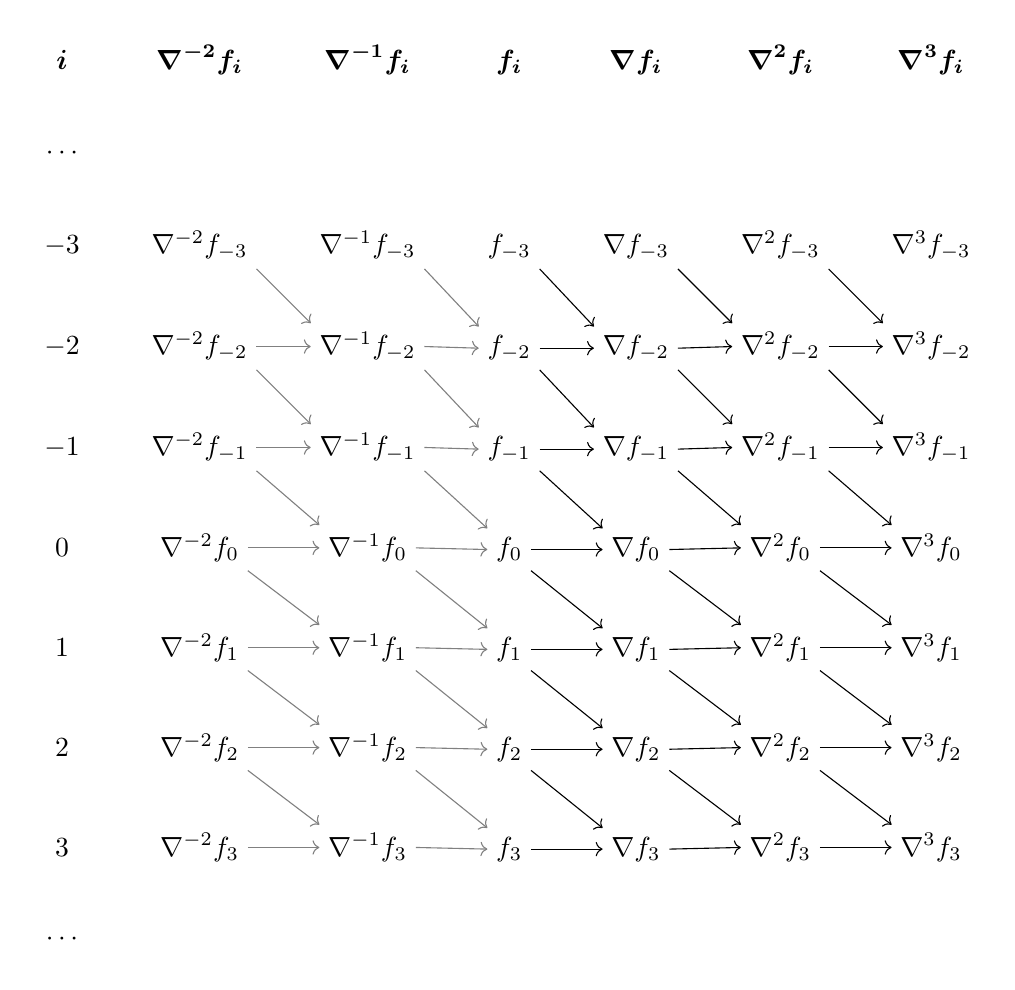
\begin{tikzpicture}
\matrix[
  matrix of math nodes,
  inner sep=3pt,
  row sep=2em,
  column sep=2em
] (M)
{
    \bm{i} & \bm{{\nabla}^{-2} f_i} & \bm{{\nabla}^{-1} f_i} & \bm{f_i} & \bm{\nabla f_i} & \bm{{\nabla}^2 f_i} & \bm{{\nabla}^3 f_i} \\
    \cdots \\
    -3 & {\nabla}^{-2} f_{-3} & {\nabla}^{-1} f_{-3} & f_{-3} &  \nabla f_{-3}  &  {\nabla}^2 f_{-3}  & {\nabla}^3 f_{-3} \\
    -2 & {\nabla}^{-2} f_{-2} & {\nabla}^{-1} f_{-2} & f_{-2} &  \nabla f_{-2}  &  {\nabla}^2 f_{-2}  & {\nabla}^3 f_{-2} \\
    -1 & {\nabla}^{-2} f_{-1} & {\nabla}^{-1} f_{-1} & f_{-1} &  \nabla f_{-1}  &  {\nabla}^2 f_{-1}  & {\nabla}^3 f_{-1} \\
     0 & {\nabla}^{-2} f_{0}  & {\nabla}^{-1} f_{0}  & f_{0}  &  \nabla f_{0}   &  {\nabla}^2 f_{0}   & {\nabla}^3 f_{0}  \\
     1 & {\nabla}^{-2} f_{1}  & {\nabla}^{-1} f_{1}  & f_{1}  &  \nabla f_{1}   &  {\nabla}^2 f_{1}   & {\nabla}^3 f_{1}  \\
     2 & {\nabla}^{-2} f_{2}  & {\nabla}^{-1} f_{2}  & f_{2}  &  \nabla f_{2}   &  {\nabla}^2 f_{2}   & {\nabla}^3 f_{2}  \\
     3 & {\nabla}^{-2} f_{3}  & {\nabla}^{-1} f_{3}  & f_{3}  &  \nabla f_{3}   &  {\nabla}^2 f_{3}   & {\nabla}^3 f_{3}  \\
    \cdots \\
}
;
\draw[->] (M-3-4.south east) -- (M-4-5.north west);
\draw[->] (M-4-4.south east) -- (M-5-5.north west);
\draw[->] (M-5-4.south east) -- (M-6-5.north west);
\draw[->] (M-6-4.south east) -- (M-7-5.north west);
\draw[->] (M-7-4.south east) -- (M-8-5.north west);
\draw[->] (M-8-4.south east) -- (M-9-5.north west);
\draw[->] (M-4-4.east) -- (M-4-5.west);
\draw[->] (M-5-4.east) -- (M-5-5.west);
\draw[->] (M-6-4.east) -- (M-6-5.west);
\draw[->] (M-7-4.east) -- (M-7-5.west);
\draw[->] (M-8-4.east) -- (M-8-5.west);
\draw[->] (M-9-4.east) -- (M-9-5.west);
\draw[->] (M-3-5.south east) -- (M-4-6.north west);
\draw[->] (M-4-5.south east) -- (M-5-6.north west);
\draw[->] (M-5-5.south east) -- (M-6-6.north west);
\draw[->] (M-6-5.south east) -- (M-7-6.north west);
\draw[->] (M-7-5.south east) -- (M-8-6.north west);
\draw[->] (M-8-5.south east) -- (M-9-6.north west);
\draw[->] (M-4-5.east) -- (M-4-6.west);
\draw[->] (M-5-5.east) -- (M-5-6.west);
\draw[->] (M-6-5.east) -- (M-6-6.west);
\draw[->] (M-7-5.east) -- (M-7-6.west);
\draw[->] (M-8-5.east) -- (M-8-6.west);
\draw[->] (M-9-5.east) -- (M-9-6.west);
\draw[->] (M-3-6.south east) -- (M-4-7.north west);
\draw[->] (M-4-6.south east) -- (M-5-7.north west);
\draw[->] (M-5-6.south east) -- (M-6-7.north west);
\draw[->] (M-6-6.south east) -- (M-7-7.north west);
\draw[->] (M-7-6.south east) -- (M-8-7.north west);
\draw[->] (M-8-6.south east) -- (M-9-7.north west);
\draw[->] (M-4-6.east) -- (M-4-7.west);
\draw[->] (M-5-6.east) -- (M-5-7.west);
\draw[->] (M-6-6.east) -- (M-6-7.west);
\draw[->] (M-7-6.east) -- (M-7-7.west);
\draw[->] (M-8-6.east) -- (M-8-7.west);
\draw[->] (M-9-6.east) -- (M-9-7.west);
\draw[gray,->] (M-3-3.south east) -- (M-4-4.north west);
\draw[gray,->] (M-4-3.south east) -- (M-5-4.north west);
\draw[gray,->] (M-5-3.south east) -- (M-6-4.north west);
\draw[gray,->] (M-6-3.south east) -- (M-7-4.north west);
\draw[gray,->] (M-7-3.south east) -- (M-8-4.north west);
\draw[gray,->] (M-8-3.south east) -- (M-9-4.north west);
\draw[gray,->] (M-4-3.east) -- (M-4-4.west);
\draw[gray,->] (M-5-3.east) -- (M-5-4.west);
\draw[gray,->] (M-6-3.east) -- (M-6-4.west);
\draw[gray,->] (M-7-3.east) -- (M-7-4.west);
\draw[gray,->] (M-8-3.east) -- (M-8-4.west);
\draw[gray,->] (M-9-3.east) -- (M-9-4.west);
\draw[gray,->] (M-3-2.south east) -- (M-4-3.north west);
\draw[gray,->] (M-4-2.south east) -- (M-5-3.north west);
\draw[gray,->] (M-5-2.south east) -- (M-6-3.north west);
\draw[gray,->] (M-6-2.south east) -- (M-7-3.north west);
\draw[gray,->] (M-7-2.south east) -- (M-8-3.north west);
\draw[gray,->] (M-8-2.south east) -- (M-9-3.north west);
\draw[gray,->] (M-4-2.east) -- (M-4-3.west);
\draw[gray,->] (M-5-2.east) -- (M-5-3.west);
\draw[gray,->] (M-6-2.east) -- (M-6-3.west);
\draw[gray,->] (M-7-2.east) -- (M-7-3.west);
\draw[gray,->] (M-8-2.east) -- (M-8-3.west);
\draw[gray,->] (M-9-2.east) -- (M-9-3.west);
\end{tikzpicture}
\caption{Backward Difference Table. The arrows in the table point towards the difference; 
the upper component is always subtracted from the lower, e.g. \( {\nabla}^2 f_3 = \nabla f_3 - \nabla f_2\)
\cite{berry2004}.}
\label{fig:differences-table-integrator}
\end{figure}

Differentiation (aka the operator \( D = d / dt \)) can be represented approximately 
in terms of  the \( E \) operator, noting that (\cite{berry2004}):
\begin{equation}
  \begin{aligned}
  E^p f(t_0 ) & = f(t_0 + p h) \\
              & = f(t_0) + p h D f(t_0) + \frac{(ph)^2}{2!}D^2f(t_0) + 
      \frac{(ph)^3}{3!}D^3f(t_0) + \ldots \\
              & = e^{phD}f(t_0)\\
  \end{aligned}
\end{equation}

We identify two operators:
\begin{equation}
  E^p = e^{phD}
\end{equation}
or taking the logarithm:
\begin{equation}
  p h D = p \log E
\end{equation}
which gives (using \ref{eq:berry6}):
\begin{equation}
  \label{eq:berry13}
  h D = \log E = - \log(1-\nabla)
\end{equation}

\section{Adams Method}
The integration operator \( D^{-1} \) can be computed as the inverse of the 
differentiation operator; using \ref{eq:berry13}:
\begin{equation}
  D^{-1} = - \frac{h}{\log(1-\nabla)}
\end{equation}

In the following, focus is placed in satellite orbits, hence the general function 
\( f \) will be replaced with \( \ddot{\vec{r}} \).

The definite integral is computed by using the diplacement operator on the indefinite 
integral (\cite{berry2004}):
\begin{equation}
  (E^p -1) D^{-1} \ddot{\vec{r}}_n = (E^p -1) \dot{\vec{r}}_n 
  = \int_{t_n}^{t_n +ph} \ddot{\vec{r}} \,dt
\end{equation}

This integration corresponds to a \emph{predictor} in a multi-step numerical 
integration, because the equation finds a value \( \dot{\vec{r}} \) at a future 
time. If \( p = 1 \), the predictor operator \( J \) can be written in terms of 
the backward difference operator as (\cite{berry2004}):
\begin{equation}
  \begin{aligned}
  J & = \frac{1}{h} (E-1) D^{-1} \\
    & = \frac{1}{h} [ {(1-\nabla)}^{-1} - 1 ] D^{-1} \\
    & = \frac{1}{h} \frac{\nabla}{1-\nabla}D^{-1} \\
    & = - \frac{\nabla}{(1-\nabla) \log(1-\nabla)}
  \end{aligned}
\end{equation}

  \chapter{Satellite Orbit modeling}
\label{ch:satellite-orbit-modeling}

\section{Quick Note: The State-Space Notation}
It is often helpfull to represent a linear differential equation in the the 
\emph{state-space} form, that is a first-order matrix differential equation of 
the form:
\begin{equation}
  \dot{\vec{x}} = \bm{F} \vec{x} + \bm{G} \vec{u} + \vec{w}
\end{equation}

where:
\begin{itemize}
  \item \(\vec{x}\) is the system \emph{state vector},
  \item \(\bm{F}\) is system's \emph{dynamic matrix},
  \item \(\vec{u}\) is a deterministic input, sometimes called a \emph{control vector}, and
  \item \(\vec{w}\) is a random forcing function, which is also known as \emph{process noise}
\end{itemize}

\section{Linearization of the Orbit Determination Process}
In the general orbit determination problem, both the dynamics and the measurements 
involve significant nonlinear relationships. For the general case, the governing 
relations involve the nonlinear expression:
\begin{subequations}
\begin{align}
  \dot{\vec{x}} = F( \vec{x}, t ), 
    & \quad \vec{x}(t_k ) \equiv \vec{x}_k 
    \label{eq:tapley421}\\
  \vec{y}_i = G( \vec{x}_i , t_i ) + {\epsilon}_i , 
    & \quad  i=1,2,\ldots ,l
    \label{eq:tapley422}
\end{align}
\end{subequations}

where \(\vec{x}_k\) is the unknown \(n\)-dimensional state vector at time \(t_k\) and 
\(\vec{y}_i\) for \(i=1,2,\ldots ,l\) is a \(p\)-dimensional set of observations. The 
\emph{best estimate} of the state vector \(\vec{x}_k\) will be denoted as \(\hat{\vec{x}}_k\). 
In general, \(p<n\) and \( m = p \times l \gg n \). The formulation described by the 
system \ref{eq:tapley421} and \ref{eq:tapley422}, is characterized by: (\cite{tapley})
\begin{enumerate}
  \item the inability to observe the state (\(\vec{x}_k\)) directly,
  \item nonlinear relations between the observations and the state, 
  \item fewer observations at any time epoch \(i\) than there are state vector 
  components (\(p<n\)), and 
  \item errors in the observations represented by \({\epsilon}_i\)
\end{enumerate}

If a reasonable reference trajectory \(\vec{x}*\) is available and if 
\(\vec{x}\), the true trajectory, and the reference trajectory remain sufficiently 
close throughout the time interval of interest, then the trajectory for the actual 
motion can be expanded in a Taylor’s series about the reference trajectory at 
each point in time. Eliminating higher order terms, the deviation in the state
from the reference trajectory can be described by a set of linear differential 
equations. Corresponding linear relations can be derived between the observation 
and the state deviations, thus transforming the nonlinear orbit determination problem 
to a linear one.

If \(\vec{\delta x}\) is the \( n \times 1 \) state deviation vector and 
\(\vec{\delta y}\) is the \(p \times 1\) observation deviation:
\begin{equation}
  \begin{aligned}
    \vec{\delta x} (t) &= \vec{x}(t) - \vec{x}^* (t) \\
    \vec{\delta y} (t) &= \vec{y}(t) - \vec{y}^*(t)
  \end{aligned}
\end{equation}

hence

\begin{equation}
  \dot{\vec{\delta x}} (t) = \dot{\vec{x}} (t) - \dot{\vec{x}}^* (t)
\end{equation}

Expanding \ref{eq:tapley421} and \ref{eq:tapley422} in a Taylor series about the 
reference trajectory, leads to:
\begin{equation}
\label{eq:tapley425}
\begin{aligned}
  \dot{\vec{x}} (t) &= F (\vec{x}, t) \\
   & \approx F (\vec{x}^* , t) 
    + \left.\frac{\partial F(t)}{\partial \vec{x}(t)}\right|_{\vec{x}^*} \left( \vec{x}(t) - \vec{x}^* (t) \right)
    + O_F \left( \vec{x}(t) - \vec{x}^* (t) \right) \\
    \vec{y}_i &= G( \vec{x}_i , t_i ) + {\epsilon}_i = \\ & \approx G( \vec{x}^*_i , t_i )
    + \left.\frac{\partial G}{\partial \vec{x}}\right|_{\vec{x}^* , i} \left.\left( \vec{x}(t_i) - \vec{x}^* (t_i) \right)\right|_{i} 
    + O_G \left( \vec{x}(t_i) - \vec{x}^* (t_i) \right) + {\epsilon}_i \\
\end{aligned}
\end{equation}

where \(\left.\frac{\partial}{\partial \vec{x}}\right|_{\vec{x}^*}\) indicates that 
the partial derivative matrix is evaluated on the reference solution \(\vec{x}^* (t)\) 
which is obtained by integrating \ref{eq:tapley421} with the initial conditions 
\(\vec{x}^* (t_0)\). \(O_F\) and \(O_G\) indicate terms higher than the 1\textsuperscript{st} 
order which are ignored. Noting that \(\dot{\vec{x}}^* = F(\vec{x}^* ,t)\) and 
\(\vec{y}^*_i = G(\vec{x}^*_i , t_i )\), and letting
\begin{subequations}
\begin{align}
\delta \vec{x}(t) & = \vec{x}(t) - \vec{x}^*(t) \label{eq:tapley426ua} \\
\delta \vec{x}_i  & = \vec{x}(t_i) - \vec{x}^*(t_i)\label{eq:tapley426ub}\\
\delta \vec{y}_i  & = \vec{y}_i - G(\vec{x}^*_i , t_i ) \label{eq:tapley426uc}
\end{align}
\end{subequations}

\ref{eq:tapley421} can be written as:
\begin{align}
  \label{eq:tapley426a}
  \delta \dot{\vec{x}}(t) &= A(t) \delta \vec{x}(t) \\
  \label{eq:tapley426b}
  \delta \vec{y}_i &= \tilde{H}_i \delta \vec{x}_i + {\epsilon}_i \quad (i=1,\ldots,l)
\end{align}

where
\begin{equation}
\label{eq:tapley426ah}
A(t) = \left.\frac{\partial F(t)}{\partial \vec{x} (t)}\right|_{\vec{x}^*} 
\quad
\tilde{H}_i = \left.\frac{\partial G}{\partial \vec{x}}\right|_{\vec{x}^* , i}
\end{equation}

\section{State Transition Matrix}
\ref{eq:tapley426a} represents a system of linear differential equations with time-dependent 
coefficients; the general solution to the system, can be expressed as:
\begin{equation}
\label{eq:tapley427}
  \bm{x}(t) = \Phi (t, t_k) \cdot \bm{x}_k \quad \text{with } \bm{x}_k = \bm{x}(t_k)
\end{equation}

The matrix \(\Phi (t_i, t_k) \) is called the \emph{state transition matrix} and has the 
following properties:
\begin{itemize}
  \item \(\Phi (t_k, t_k) = I \)
  \item \(\Phi (t_i, t_k) = \Phi (t_i, t_j) \Phi (t_j, t_k) \)
  \item \(\Phi (t_i, t_k) = {\Phi}^{-1} (t_j, t_k) \)
\end{itemize}

Noting that \(\bm{x}_k\) is constant,
\begin{equation}
  \label{eq:tapley429}
  \bm{\dot{x}}(t) = \dot{\Phi} (t, t_k) \cdot \bm{x}_k
\end{equation}

Using \ref{eq:tapley426a} and \ref{eq:tapley427},
\begin{equation}
  \label{eq:tapley4210}
  \begin{aligned}
  \dot{\Phi} (t, t_k) \bm{x}_k & = A(t) \cdot \bm{x} (t) \\
  & = A(t) \cdot \Phi (t, t_k) \bm{x}_k \\ 
  \implies & \dot{\Phi} (t, t_k) = A(t) \Phi (t, t_k)
  \end{aligned}
\end{equation}

\ref{eq:tapley4210} represents a linear differential equation. For any practical orbit 
determination application, the solution for \(\Phi (t, t_0)\)  will be obtained
via numerical integration, supplying a vector of derivative values for the differential 
equation of the nominal state vector and computed values for \(\dot{\Phi} (t, t_0)\).

\section{Observations}
Combining \ref{eq:tapley427} and \ref{eq:tapley426b}, we get:
\begin{equation}
  \label{eq:tapley4237}
  \begin{aligned}
    \bm{y}_0 &= \tilde{H}_0 \Phi (t_0, t_k) \bm{x}_k + {\epsilon}_0 \\
    \bm{y}_1 &= \tilde{H}_1 \Phi (t_1, t_k) \bm{x}_k + {\epsilon}_1 \\
    & \vdotswithin{=} \\
    \bm{y}_{l-1} &= \tilde{H}_{l-1} \Phi (t_{l-1}, t_k) \bm{x}_k + {\epsilon}_{l-1}
  \end{aligned}
\end{equation}

where the system contains \(m=p\times l\) observations and \(n\) unknown components 
in the state vector. For convinience, we define the following notation:
\begin{equation}
  \bm{y} \equiv \begin{bmatrix} y_0 \\ y_1 \\ \ldots \\ y_{l-1} \end{bmatrix},
  \quad
  H \equiv \begin{bmatrix} \tilde{H}_0 \Phi (t_0, t_k) \\ \tilde{H}_1 \Phi (t_1, t_k) \\ \ldots \\ \tilde{H}_{l-1} \Phi (t_{l-1}, t_k) \end{bmatrix},
  \quad
  \bm{\epsilon} \equiv \begin{bmatrix} {\epsilon}_0 \\ {\epsilon}_1 \\ \ldots \\ {\epsilon}_{l-1} \end{bmatrix}
\end{equation}

so that we can now write \ref{eq:tapley4237} as:
\begin{equation}
  \label{eq:tapley4239}
  \bm{y} = H \bm{x} + \bm{\epsilon} 
  \quad
  \bm{y} \in \mathbb{R} ^{m \times 1},
  \bm{x} \in \mathbb{R} ^{n \times 1},
  H \in \mathbb{R}^{m \times n},
\end{equation}

where \( m = p \times l \) is the total number of observations.

\section{Sequential Estimation Overview}
In the sequential estimation algorithm, observations are processed as soon as they 
are received (in contrast to batch estimation), thus offering the advantage of 
inverting a matrix of the same dimension as the observation vector. Hence, if the 
observations are processed individually, only scalar divisions will be required to 
obtain the estimate of \(\vec{x}_k\). The sequential estimation algorithm discussed 
here, is often reffered to as the \emph{Kalman filter}, named after Rudolf E. K\'alm\'an
who was one of the primary developers of its theory. 

An estimate \(\hat{\bm{x}}_j \) and a covariance matrix \(P_j\) can be 
propagated forward to an epoch \(t_k\) by the relations (known as the 
\emph{time update} equations)
\begin{subequations}
\label{eq:tapley471}
\begin{align}
  \bar{\bm{x}} _k & = \Phi (t_k, t_j) \hat{\bm{x}}_j 
  \label{eq:tapley471a}\\
  \bar{P}_k & = \Phi (t_k, t_j) P_j \Phi ^T (t_k, t_j)
  \label{eq:tapley471b}
\end{align}
\end{subequations}


Assume that we have a new, additional obervation at epoch \(t_k\),
\begin{equation}
  \bm{y}_k = \tilde{H}_k \bm{x}_k + \bm{\epsilon} _k ,
  \quad E\left[\bm{\epsilon} _k \right] = 0,
  \quad E\left[\bm{\epsilon} _k \bm{\epsilon} ^T_j \right] = R_k \delta _{kj}
\end{equation}

(where \(\delta _{kj}\) is the \emph{Kronicker delta}). We wish to process 
\(\bm{y} _k\) in order to determine \(\hat{\bm{x}} _k\). The best estimate of 
\(\bm{x} _k\) is

\begin{equation}
\label{eq:tapley473}
\hat{\bm{x}} _k = \left( \tilde{H}^T_k R^{-1}_k \tilde{H}_k + \bar{P}^{-1}_k \right)^{-1} \left( \tilde{H}^T_k R^{-1}_k \bm{y}_k + \bar{P}^{-1}_k \bar{\bm{x}}_k \right)
\end{equation}

\ref{eq:tapley473} implies the inversion of the \(n \times n\) \emph{information matrix} \(\Lambda _k\), 
\begin{equation}
\label{eq:tapley474}
\Lambda ^{-1}_k = P_k = 
\left( \tilde{H}^T_k R^{-1}_k \tilde{H}_k + \bar{P}^{-1}_k \right)^{-1}
\end{equation}

From \ref{eq:tapley474}, it follows that:
\begin{equation}
  \label{eq:tapley475}
  P^{-1}_k  
    = \tilde{H}^T_k R^{-1}_k \tilde{H}_k + \bar{P}^{-1}_k
\end{equation}

Premultiplying each side of \ref{eq:tapley475} by \(P_k\) and then postmultiplying 
by \(\bar{P}_k\), leads to:
\begin{subequations}
\begin{align}
  \bar{P}_k &= 
    P_k \tilde{H}^T_k R^{-1}_k \tilde{H}_k \bar{P}_k + P_k 
      \quad or \label{eq:tapley476} \\
  P_k &= 
    \bar{P}_k - P_k \tilde{H}^T_k R^{-1}_k \tilde{H}_k \bar{P}_k 
      \label{eq:tapley477}
  \end{align}
\end{subequations}

Postmultiplying \ref{eq:tapley476} by \(\tilde{H}^T_k R^{-1}_k\)
\begin{equation}
  \label{eq:tapley478}
  \begin{aligned}
  \bar{P}_k \tilde{H}^T_k R^{-1}_k &= 
    P_k \tilde{H}^T_k R^{-1}_k \tilde{H}_k \bar{P}_k \tilde{H}^T_k R^{-1}_k +
    P_k \tilde{H}^T_k R^{-1}_k & \\
  &= P_k \tilde{H}^T_k R^{-1}_k \left(
    \tilde{H}_k \bar{P}_k \tilde{H}^T_k R^{-1}_k + I \right) & \\
  &= P_k \tilde{H}^T_k R^{-1}_k \left(
     \tilde{H}_k \bar{P}_k \tilde{H}^T_k + R_k \right) R^{-1}_k &
  \end{aligned}
\end{equation}

We can postmultiply \ref{eq:tapley478} by \(R_k\) and then by 
\(\left(\tilde{H}_k \bar{P}_k \tilde{H}^T_k + R_k \right) ^{-1} \) to solve for 
the quantity \(P_k \tilde{H}^T_k R^{-1}_k\):
\begin{equation}
\label{eq:tapley479}
P_k \tilde{H}^T_k R^{-1}_k = 
\bar{P}_k \tilde{H}^T_k \left( \tilde{H}_k \bar{P}_k \tilde{H}^T_k + R_k \right) ^{-1}
\end{equation}

which relates the \emph{a-priori} covariance matrix \(\bar{P}_k\) to the 
\emph{a-posteriori} covariance matrix \(P_k\).

Substituting \ref{eq:tapley479} into \ref{eq:tapley477}, yields:
\begin{equation}
\label{eq:tapley4710}
  P_k = 
    \bar{P}_k - \bar{P}_k \tilde{H}^T_k \left( \tilde{H}_k \bar{P}_k \tilde{H}^T_k + R_k \right) ^{-1} \tilde{H}_k \bar{P}_k 
\end{equation}

\ref{eq:tapley4710} is an alternate way of computing the inverse in \ref{eq:tapley474}, 
but here the matrix to be inverted is of dimension \(p \times p\), that is the 
same dimensions as the observation error covariance matrix. If the observations are 
processed as scalars (i.e. one at a time), only a scalar division is required.

If we define the weighting matrix \(K_k\), usually called \emph{Kalman gain matrix}, 
as
%\begin{equation}
\begin{tcolorbox}[ams equation]
\label{eq:tapley4711}
K_k = \bar{P}_k \tilde{H}^T_k \left( \tilde{H}_k \bar{P}_k \tilde{H}^T_k + R_k \right) ^{-1}
\end{tcolorbox}
%\end{equation}

then \ref{eq:tapley4710} reads
%\begin{equation}
\begin{tcolorbox}[ams equation]
\label{eq:tapley4712}
P_k = \left( I - K_k \tilde{H}_k \right) \bar{P}_k
\end{tcolorbox}
%\end{equation}

Note also, that substituting \ref{eq:tapley479} into \ref{eq:tapley4711}, we get
\begin{equation}
\label{eq:tapley4714}
K_k = P_k \tilde{H}^T_k R^{-1}_k
\end{equation}

Substituting \ref{eq:tapley474} into \ref{eq:tapley473}, we get:
\begin{equation}
  \begin{aligned}
  \hat{\bm{x}}_k &= P_k 
    \left( \tilde{H}^T_k R^{-1}_k \bm{y}_k + \bar{P}^{-1}_k \bar{\bm{x}}_k \right) \\
  & = \underbrace{P_k \tilde{H}^T_k R^{-1}_k}_{K_k} \bm{y}_k + P_k \bar{P}^{-1}_k \bar{\bm{x}}_k  \\
  & = K_k \bm{y}_k + P_k \bar{P}^{-1}_k \bar{\bm{x}}_k \\
  & = K_k \bm{y}_k + \left( I - K_k \tilde{H}_k \right) \bar{P}_k \bar{P}^{-1}_k \bar{\bm{x}}_k
  \end{aligned}
\end{equation}

and finaly
%\begin{equation}
\begin{tcolorbox}[ams equation]
\label{eq:tapley4716}
\hat{\bm{x}}_k = \bar{\bm{x}}_k + K_k \left( \bm{y}_k - \tilde{H}_k \bar{\bm{x}}_k \right)
\end{tcolorbox}
%\end{equation}

\ref{eq:tapley4711}, \ref{eq:tapley4712}, \ref{eq:tapley4716} along with \ref{eq:tapley471} can be used in a recursive fashion to compute the estimate \(\hat{\bm{x}}_k\) 
incorporating the observation \(\bm{y}_k\).

\subsection{Sequential Estimation Algorithm}
\label{ssec:sequential-estimation-algorithm}
Given the initial conditions \(\vec{X}^*_{k-1}\), \(\hat{\bm{x}}_{k-1}\) and \(P_{k-1}\), 
the observation \(Y_k\) and the corresponding \(R_k\) at \(t=t_k\), the algorithm 
for computing the estimate sequentially is summarized as:
\begin{enumerate}
  \item \label{en:kalman-wf-item1} Integrate reference trajectory (\(X^*\)) and 
  state transition matrix, from \(t_{k-1}\) to \(t_k\) (see \ref{eq:tapley421}, \ref{eq:tapley426ah} and \ref{eq:tapley4210})
    \begin{subequations}
    \begin{align}
      \dot{X}^* &= F( X^* , t ) 
        \quad \text{with initial conditions } X^*_{k-1} \label{eq:tapley4717a} \\
      A(t) &= 
        \left.\frac{\partial F(X,t)}{\partial X}\right|_{X=X^*} \\
      \dot{\Phi} (t, t_{k-1}) &= 
        A(t) \Phi (t,t_{k-1}) 
        \quad \text{with initial conditions } \Phi(t_{k-1}, t_{k-1}) = I\label{eq:tapley4717b}
    \end{align}
    \end{subequations}
    This step results in computation of \(X^*_{t_k}\) and \(\Phi (t_k, t_{k-1})\)

  \item \label{en:kalman-wf-time-update} Compute the time update (see \ref{eq:tapley471}):
    \begin{subequations}
    \begin{align}
      \bar{\bm{x}}_k &= \Phi (t_k , t_{k-1}) \hat{\bm{x}}_{k-1} \\
      \bar{P}_k &= \Phi (t_k , t_{k-1}) P_{k-1} \Phi ^T (t_k , t_{k-1})
    \end{align}
    \end{subequations}

  \item Compute observation deviation, observation state matrix and gain matrix (see \ref{eq:tapley426uc}, \ref{eq:tapley426ah} and \ref{eq:tapley4711})
    \begin{subequations}
    \begin{align}
      \bm{y}_k &= Y_k - G(X^*_k , t_k ) \\
      \tilde{H}_k &= \left.\frac{\partial G(X , t_k )}{\partial X} \right|_{X=X^*} \\
      K_k & = 
        \bar{P}_k \tilde{H}^T_k 
          \left( \tilde{H}_k \bar{P}_k \tilde{H}^T_k + R_k \right) ^{-1}
    \end{align}
    \end{subequations}

  \item Compute the \emph{measurement update} (see \ref{eq:tapley4712} and \ref{eq:tapley4716})
    \begin{subequations}
    \begin{align}
\hat{\bm{x}}_k &= \bar{\bm{x}}_k + K_k \left( \bm{y}_k - \tilde{H}_k \bar{\bm{x}}_k \right) \\
P_k &= \left( I - K_k \tilde{H}_k \right) \bar{P}_k
    \end{align}
    \end{subequations}

  \item Replace \(k\) with \(k+1\); \(X^*(t_k)\) now becomes \(X^*(t_{k-1})\).
  Return to \ref{en:kalman-wf-item1}.

\end{enumerate}

The estimate of the state of the nonlinear system at \(t_k\) is given by 
\(\hat{X}_k = X^*_k + \hat{\bm{x}}_k\)

Note that if there is an observation at \(t_0\), a time update (\ref{en:kalman-wf-time-update}) is not performed but a measurement update is performed.

Also, note that the differential equations for the state transition matrix
are reinitialized at each observation epoch. Therefore, the state transition matrix
is reinitialized at each observation epoch. If there is more than one observation
at each epoch and we are processing them as scalars, we would set \(\Phi (t_i , t_i ) = I\)
after processing the first observation at each epoch; \(P\) and \(\hat{\bm{x}}\) are not
time updated until we move to the next observation epoch. 

\subsection{Shortcomings and Considerations}
One disadvantage of the sequential algorithm lies in the fact that if the true state 
and the reference state are not close together then the linearization assumption 
leading to \ref{eq:tapley426} may not be valid and the estimation process may diverge.
This problem can be adressed via the \emph{extended sequential filter algorithm}, see 
\cite{tapley}.

A second unfavorable characteristic of the sequential estimation algorithm is
that the state estimation error covariance matrix may approach zero as the number
of observations becomes large. The trace of the state estimation error covariance 
matrix grows between observations and is reduced by the amount \(trace(K\tilde{H}\bar{P})\) 
after each observation. Hence, the magnitude of the covariance matrix elements 
will decrease depending on the density, information content, and accuracy of the 
observations.

Examination of the estimation algorithm shows that as \(P_k \to 0\), the gain 
approaches zero, and the estimation procedure will become insensitive to the 
observations. Consequently, the estimate will diverge due to either errors introduced 
in the linearization procedure, computational errors, or errors due to an incomplete 
mathematical model. To overcome this problem, process noise often is added to 
the state propagation equations.

In addition to these two problems, the Kalman filter may diverge because of
numerical difficulties associated with the covariance measurement update, given by 
\ref{eq:tapley4712}. The covariance matrix may lose its properties of symmetry and 
become nonpositive definite when the computations are carried out with the finite 
digit arithmetic of the computer. In particular, this equation can fail to yield a 
symmetric positive definite result when a large a priori covariance is reduced by 
the incorporation of very accurate observation data (\cite{tapley}). The most common 
solution to numerical problems with the covariance update is to use a square root 
formulation to update the covariance matrix (\ref{sec:square-root-filtering}).

\subsection{The Extended Sequential Estimation Algorithm}
To minimize the effects of errors due to the neglect of higher order terms in the
linearization procedure leading \ref{eq:tapley426}, the extended form of the sequential
estimation algorithm is sometimes used. This algorithm is often referred to as the
\emph{Extended Kalman Filter} (EKF). The primary difference between the sequential
and the extended sequential algorithm is that the reference trajectory for the ex-
tended sequential algorithm is updated after each observation to reflect the best
estimate of the true trajectory. For example, after processing the \(k^{th}\) observation, 
the best estimate of the state vector at \(t_k\) is used to provide new initial 
conditions for the reference trajectory,
\begin{equation}
  X^*_{k,new} = \hat{X}_k = X^*_k + \hat{\bm{x}}_k
\end{equation}

The flowchart for the \emph{Extended Sequential Estimation Aalgorithm} is given below, 
in contrast to the one presented in \ref{ssec:sequential-estimation-algorithm}.

Given the initial conditions \(\vec{X}^*_{k-1}\), \(\hat{\bm{x}}_{k-1}\) and \(P_{k-1}\), 
the observation \(Y_k\) and the corresponding \(R_k\) at \(t=t_k\), the algorithm 
for computing the estimate sequentially is summarized as:
\begin{enumerate}
  \item \label{en:kalman-wf-item1} Integrate reference trajectory (\(X^*\)) and 
  state transition matrix, from \(t_{k-1}\) to \(t_k\) (see \ref{eq:tapley421}, \ref{eq:tapley4210})
    \begin{subequations}
    \begin{align}
      \dot{X}^* &= F( X^* , t ) 
        \quad \text{with initial conditions } X^*_{k-1} \label{eq:tapley4717a} \\
      A(t) &= 
        \left.\frac{\partial F(X,t)}{\partial X}\right|_{X=X^*} \\
      \dot{\Phi} (t, t_{k-1}) &= 
        A(t) \Phi (t,t_{k-1}) 
        \quad \text{with initial conditions } \Phi(t_{k-1}, t_{k-1}) = I\label{eq:tapley4717b}
    \end{align}
    \end{subequations}
    This step results in computation of \(X^*_{t_k}\) and \(\Phi (t_k, t_{k-1})\)

  \item \label{en:kalman-wf-time-update} Compute the time update (see \ref{eq:tapley471b}); \textcolor{red}{in contrast to the sequential estimation filter, the extended version does not use \ref{eq:tapley471a} at this step}
    \begin{subequations}
    \begin{gather}
      \hcancel[red]{\bar{\bm{x}}_k = \Phi (t_k , t_{k-1}) \hat{\bm{x}}_{k-1}} \\
      \bar{P}_k = \Phi (t_k , t_{k-1}) P_{k-1} \Phi ^T (t_k , t_{k-1})
    \end{gather}
    \end{subequations}

  \item Compute observation deviation, observation state matrix and gain matrix (see \ref{eq:tapley426uc}, and \ref{eq:tapley426ah})
    \begin{subequations}
    \begin{align}
      \bm{y}_k &= Y_k - G(X^*_k , t_k ) \\
      \tilde{H}_k &= \frac{\partial G(X^*_k , t_k )}{\partial X} \\
      K_k & = 
        \bar{P}_k \tilde{H}^T_k 
          \left( \tilde{H}_k \bar{P}_k \tilde{H}^T_k + R_k \right) ^{-1}
    \end{align}
    \end{subequations}

  \item Compute the measurement \textcolor{red}{and reference orbit} update (see \ref{eq:tapley4711}, \ref{eq:tapley4712}, \ref{eq:tapley4716})
    \begin{subequations}
    \begin{gather}
      \hcancel{\hat{\bm{x}}_k = \bar{\bm{x}}_k + K_k \left( \bm{y}_k - \tilde{H}_k \bar{\bm{x}}_k \right)} \\
      \textcolor{red}{\hat{\bm{x}} = K_k \bm{y}_k} \\
      \textcolor{red}{X^*_k = X^*_k + \hat{\bm{x}}} \\
      P_k = \left( I - K_k \tilde{H}_k \right) \bar{P}_k
    \end{gather}
    \end{subequations}

  \item Replace \(k\) with \(k+1\); \(X^*(t_k)\) now becomes \(X^*(t_{k-1})\).
  Return to \ref{en:kalman-wf-item1}.

\end{enumerate}

The estimate of the state of the nonlinear system at \(t_k\) is given by 
\(\hat{X}_k = X^*_k + \hat{\bm{x}}_k\)

\subsection{The Prediction Residual}
It is of interest to examine the variance of the predicted residuals, which are
sometimes referred to as the \emph{innovation}, or \emph{new information}, which 
comes from each measurement. The predicted residual, or innovation, is the observation 
residual based on the a-priori or predicted state, \(\bar{\bm{x}}\), at the observation 
time, \(t_k\), and is defined as
\begin{equation}
  \label{eq:tapley4733}
  \beta _k = \bm{y}_k - \tilde{H}_k \bar{\bm{x}}_k
\end{equation}

with
\begin{equation}
  \begin{aligned}
    \bar{\bm{x}}_k &= \bm{x}_k + \eta _k \\
    \bm{y}_k &= \tilde{H}_k \bm{x}_k + \epsilon _k
  \end{aligned}
\end{equation}

where \(\bm{x}_k\) is the true value of the state deviation vector and \(\bm{\eta}_k\) 
is the error in \(\bar{\bm{x}}\). Also
\begin{equation}
  E \left[ \bm{\eta}_k \right] = 0, \quad 
  E \left[ \bm{\eta}_k , \bm{\eta}^T_k \right] = \bar{P}_k
\end{equation}

and
\begin{equation}
  \begin{aligned}
  E \left[ \bm{\epsilon}_k \right] &= 0 \\
  E \left[ \bm{\epsilon}_k , \bm{\epsilon}^T_k \right] &= R_k \\
  E \left[ \bm{\epsilon}_k , \bm{\eta}^T_k \right] &= 0
  \end{aligned}
\end{equation}

From these conditions it follows that \(\beta _k\) has mean
\begin{equation}
  \begin{aligned}
    E \left[ \beta _k \right] \equiv \bar{\beta}_k &= E \left[
      \tilde{H}_k \bm{x}_k + \epsilon _k - \tilde{H}_k \bar{\bm{x}}_k \right] \\
    &= E \left[ \tilde{H}_k \left( \bm{x}_k - \bar{\bm{x}}_k \right) + \epsilon _k \right] \\
    & = E \left[ \epsilon _k - \tilde{H}_k \bm{\eta}_k \right] \\
    & = 0
  \end{aligned}
\end{equation}

and variance-covariance
\begin{equation}
  \begin{aligned}
    P_{\beta _k} &= 
      E \left[ \left( \beta _k - \bar{\beta}_k \right) \left( \beta _k - \bar{\beta}_k \right)^T \right] \\
    & = E \left[ \beta _k {\beta}^T_k \right] \\
    & = E \left[ \left( \bm{y}_k - \tilde{H}_k \bar{\bm{x}}_k \right) 
      \left( \bm{y}_k - \tilde{H}_k \bar{\bm{x}}_k \right)^T \right] \\
    & = E \left[ \left( \bm{\epsilon}_k - \tilde{H}_k \bm{\eta}_k \right)
      \left( \bm{\epsilon}_k - \tilde{H}_k \bm{\eta}_k \right)^T \right] \\
    & = R_k + \tilde{H}_k \bar{P}_k \tilde{H}^T_k
  \end{aligned}
\end{equation}

Using formula \ref{eq:tapley:4711}, we can write the gain matrix \(K_k\) in terms 
of the residual variance-covariance
\begin{equation}
  \begin{aligned}
  K_k &= 
    \bar{P}_k \tilde{H}^T_k \left( \tilde{H}_k \bar{P}_k \tilde{H}^T_k + R_k \right) ^{-1} \\
  &=
    \bar{P}_k \tilde{H}^T_k P_{\beta _k}^{-1}
  \end{aligned}
\end{equation}

Hence, for a large prediction residual variance-covariance, the Kalman gain matrix 
will be small and the observation will have little influence on the estimate of the 
state. Also, large values of the prediction residual relative to the prediction residual 
standard deviation, may be an indication of bad tracking data and hence may be used to 
edit data from the solution.

\section{State Noise}
In addition to the effects of the nonlinearities, the effects of errors in the dynamical 
model can lead to divergence in the estimate. As pointed out previously, for a sufficiently large
number of observations the elements of the covariance matrix \(P_k\) will asymptotically 
approach zero and the estimation algorithm will be insensitive to any further
observations. This condition can lead to filter divergence. One approach to preventing 
this divergence is to recognize that the linearized equations for propagating the 
estimate of the state are in error and to compensate for this by assuming
that the error in the linearized dynamics can be approximated by process noise.

The state dynamics of a linear system under the influence of process noise are
described by:
\begin{equation}
  \label{eq:tapley491}
  \dot{\bm{x}} (t) = A(t) \bm{x} (t) + \Beta (t) \bm{u} (t)
\end{equation}

Where the vector \(\bm{u}\), called the \emph{state} or \emph{process noise} is of 
dimension \(m \times 1 \) and the matrix \(\Beta \) is \(n \times m \).
The functional form of \(\bm{u}\) can include a number of processes, including constant, 
piecewise constant, correlated, or white noise.

If we assume a white process noise:
\begin{equation}
  \label{eq:tapley492}
  \begin{aligned}
    E \left[ \bm{u} (t) \right] &= 0 \\
    E \left[ \bm{u} (t) \bm{u}^T (\tau) \right] &= Q(t) \delta (t-\tau)
  \end{aligned}
\end{equation}
where \(\delta (t-\tau)\) is the \emph{Dirac Delta} and \(Q\) is called the 
\emph{process noise covariance matrix}. The algorithm that results from the assumption 
that \( \bm{u} (t) \) is white noise with known covariance is known as \gls{snc}. 
The use of more sophisticated models such as the process to compensate for state 
and/or measurement model errors generally is referred to as \gls{dmc}.

The solution of \ref{eq:tapley491}, is given by (for a detailed description, see \cite{tapley})
\begin{equation}
  \label{eq:tapley4914}
  \bm{x} (t) = \Phi(t, t_0) \bm{x}_0 + 
    \int_{t_0}^{t} \Phi(t, \tau ) \Beta (\tau ) \bm{u} (\tau ) \, d\tau 
\end{equation}
which is the general solution for the inhomogeneous \ref{eq:tapley491} and
indicates how the true state propagates under the influence of process noise.

If the mean of the process noise is zero, that is \(E \left[ \bm{u} (t) \right] = 0 \), 
then the equation for propagating the state estimate is the same as without process noise
(\cite{tapley})
\begin{equation}
  \label{eq:tapley4919}
  \bar{\bm{x}} (t) = \Phi (t , t_{k-1} ) \hat{\bm{x}}_{k-1}
\end{equation}

One could derive a solution for the case where the mean is nonzero. In the case 
where \(E \left[ \bm{u} (t) \right] = \bar{\bm{u}} \), 
the solution would be obtained by applying the expectation operator to \ref{eq:tapley492} 
to yield
\begin{equation}
  \label{eq:tapley4920}
  \bar{\bm{x}} (t) = \Phi (t , t_{k-1} ) \hat{\bm{x}}_{k-1} + \Gamma (t , t_{k-1} ) \bar{\bm{u}}
\end{equation}
where \(\Gamma (t , t_{k-1} )\) is given by \ref{eq:tapley4947}.

\begin{equation}
  \label{eq:tapley4944}
  \bar{P}(t) = \Phi (t , t_{k-1} ) P_{k-1} \Phi ^T (t , t_{k-1} )
    +  \int_{t_{k-1}}^{t} \Phi(t, \tau ) \Beta (\tau ) Q (\tau ) \Beta ^T (\tau ) \Phi ^T (t, \tau ) \, d\tau
\end{equation}

\section{Square Root Filtering}
\label{sec:square-root-filtering}
Sequential estimation algorithms are subject to the filter divergence phenomenon, during 
which the estimate of the state can depart in an unbounded manner from the true value 
of the state. There are two fundamental reasons for filter divergence (\cite{tapley}):
\begin{itemize}
  \item due to inaccuracies in the mathematical model used to describe the dynamic 
  process or in the model used to relate the observations to the state, and
  \item the state error covariance matrix during measurement update can become nonpositive 
  definite (a situation that is a theoretical impossibility) due to floating point 
  arithmetic when computing the update of the state error covariance matrix at the 
  point where an observation is incorporated \footnote{When the eigenvalues have a wide spread, the error
introduced in the computational process can destroy the symmetry and positive
definite character of the covariance matrix and filte r divergence may occur, see \cite{tapley}.}.
\end{itemize}

The latter point is addressed in modifications of the computational algorithm called 
\emph{square root covariance filters}, in which the state error covariance matrix is 
replaced by its square root. The state error covariance matrix is obtained by
multiplying the square root matrix by its transpose and will always be symmetric
and positive semidefinite.

If we define
\begin{equation}
\label{eq:tapley571}
P = W W^T
\end{equation}

where \(W\) is the state error covariance matrix square root, and use \ref{eq:tapley571} to 
compute the \(P\) matrix, this can never be nonpositive definite even in the presence 
of round-off or truncation errors. Furthermore, since \(P\) is symmetric and positive 
definite, there will exist an orthogonal matrix \(M\) such that:
\begin{equation}
\label{eq:tapley572}
  P^* = M^T P M
\end{equation}

where \(P^*\) is a diagonal matrix whose elements are the eigenvalues of \(P\) and 
\(M\) is the corresponding matrix of eigenvectors. Define \(W^*\) as the matrix 
whose diagonal elements are equal to the square root of the diagonal elements of \(P^*\)
\begin{equation}
  W^*_{ii} = \sqrt P^*_{ii} \quad i=1,\ldots ,n
\end{equation}
where \(P^*_{ii} > 0\), then
\begin{equation}
 W^* W^{*T} = P^* = M^T P M = M^T W W^T M
\end{equation}

Thus, \(W^* = M^T W \) and since \(M\) is an orthogonal matrix, it follows that
\begin{equation}
  \label{eq:tapley574}
  W = M W^*
\end{equation}

The numerical conditioning of \(W\) is generally much better than that of \(P\) (see 
e.g. \cite{lawson1995}, \cite{tapley}).

  \chapter{Time, Time Scales and Calendars}
\label{ch:time-scales}

\section{Julian Date and Modified Julian Date}
\label{sec:julian-date}
Calendar dates are usually quaite cumbersome and inefficient to use when 
performing date computations; instead, a continuous count of days is prefered. 
To this end, the \emph{Julian day number} was introduced with JD zero located 
about 7000 years ago (for example Julian day number 2449444 began at noon on 
1994 April 1). Note that JD (and MJD) can be used in conjunction to most 
time scales used in astronomy, such as TAI, TT and TDB.

\emph{Julian Date} (JD) is the same system but with a fractional part appended; JD 2449443.5 was the
midnight on which 1994 April 1 commenced (\cite{sofa_18161_tscb}). Removing the leading 
`24' and dropping the fractional `.5' part, yileds the so called \emph{Modified Julian Date}, 
aka:
\begin{equation}
    MJD = JD - 2400000.5
\end{equation}
Thus 1994 April 1 commenced at MJD 49443.0. Within \ref{ssec:dso-datetime}, dates are 
internally stored as MJD (integers).

\subsection{Julian Epoch}
It is often convinient to work with fractional years; in the past, this was done 
using a system called \emph{Besselian epoch} (\cite{sofa_18161_tscb}) but since the 
mid-80's, the \emph{Julian epoch} took over. It uses the Julian year of exactly 365.25 days,
and the TT time scale. Julian epoch 2000.0 is defined to be 2000 January 1.5, which
is JD 2451545.0 or MJD 51544.5 (\cite{sofa_18161_tscb}). Julian epochs are denoted with 
a `J' prefix, hence e.g. `J2000.0' is Julian epoch 2000.0.

\section{Time Scales}
The most common time scales used in astronomical computations, are:
\begin{table}
  \centering
\begin{tabularx}{\textwidth}{>{\raggedright\arraybackslash}X >{\raggedright\arraybackslash}X c}
  %\hline
    \bf{Time-Scale} & \bf{Description} & \bf{Type} \\
  \hline
  \textbf{TAI}\\ \scriptsize{(International Atomic Time)} & The official timekeeping standard & Atomic \\
  \textbf{UTC}\\ \scriptsize{(Coordinated Universal Time)} & The basis of civil time & Atomic/Solar hybrid \\
  \textbf{UT1}\\ \scriptsize{(Universal Time)} & Based on Earth rotation & Solar \\
  \textbf{TT}\\ \scriptsize{(Terrestrial Time)} & Used for solar system ephemeris look-up &  Dynamic \\
  \textbf{TCG}\\ \scriptsize{(Geocentric Coordinate Time)} & Used for calculations centered on the Earth in space & Dynamic \\
  \textbf{TCB}\\ \scriptsize{(Barycentric Coordinate Time)} & Used for calculations beyond Earth orbit; for most common cases, may be approximated by \textbf{TT} & Dynamic \\
  \textbf{TDB}\\ \scriptsize{(Barycentric Dynamical Time)} & A scaled form of TCB that keeps in step with TT
on the average & Dynamic \\
  %\hline
\end{tabularx}
\caption{Common Time Scales used in Astronomical and Celestial Computations.}
\end{table}

Time scales that are obsolete, according to \cite{sofa_18161_tscb}, are:
\begin{description}
  \item[UT0, UT2]: specialist forms of universal time that take into account polar motion and
known seasonal effects; no longer used.
  \item[GMT] (Greenwich mean time): an obsolete time scale that can be taken to mean either
UTC or UT1.
  \item[ET] (ephemeris time): superseded by TT and TDB.
  \item[TDT] (terrestrial dynamical time): the former name of TT.
\end{description}

Note that \emph{Sidereal time} ins not really a time scale but rather an angle. 
The same can be said of UT1; however, the interrelation between UTC and UT1 makes 
it clearer and more convenient to treat the latter as a time scale.

Each of the time scales Each has a distinct role, and there are offsets of tens 
of seconds between some of them. The transformation from one time scale to the next can take a number of forms. In some cases,
for example TAI to TT, it is simply a fixed offset. In others, for example TAI to UT1, it is
an offset that depends on observations and cannot be predicted in advance (or only partially).
Some time scales, for example TT and TCG, are linearly related, with a rate change as well as an
offset. Others, for example TCG and TCB, require a 4-dimensional spacetime transformation (\cite{sofa_18161_tscb}).

\begin{figure}
\centering
\begin{tikzpicture}
\coordinate (TAI) at (-4,5.0);
\coordinate (UTC) at (-4,2.5);
\coordinate (UT1) at (-4,0);
\coordinate (TT) at (0,0);
\coordinate (TCG) at (2,-2.5);
\coordinate (TCB) at (2,-5.0);
\coordinate (TDB) at (2,-7.5);

\draw [thick] (UT1) rectangle node{\textbf{UT1}}  ($(UT1)+(1.4,0.8)$);
\draw [thick] (UTC) rectangle node{\textbf{UTC}}  ($(UTC)+(1.4,0.8)$);
\draw [thick] (TAI) rectangle node{\textbf{TAI}}  ($(TAI)+(1.4,0.8)$);
\draw [thick] (TT)  rectangle node{\textbf{TT}}   ($(TT)+(1.4,0.8)$);
\draw [thick] (TCG) rectangle node{\textbf{TCG}}  ($(TCG)+(1.4,0.8)$);
\draw [thick] (TCB) rectangle node{\textbf{TCB}}  ($(TCB)+(1.4,0.8)$);
\draw [thick] (TDB) rectangle node{\textbf{TDB}}  ($(TDB)+(1.4,0.8)$);

\draw [blue,thick,->] ($(TAI) + (0.7,0.0)$) -- node[anchor=west]{\(-\Delta AT\) (leap seconds)} ($(UTC) + (0.7,+0.8)$);
\draw [red,thick,->] ($(UTC) + (0.7,0.0)$) -- node[anchor=west]{\(+\Delta UT1\)} ($(UT1) + (0.7,+0.8)$);
\path [>=latex,->,draw,red,thick] ($(TAI) + (0.0,+0.3)$) -| ++(-1,-2.5) node[rotate=90,above]{\(+\textcolor{red}{\Delta UT1} - \textcolor{blue}{\Delta AT} \)} |- ($(UT1)+(0.0,+0.3)$);
\path [>=latex,->,draw,blue,thick] ($(TAI) + (1.4,+0.3)$) -| ++(3.8,-2.3) node[rotate=90,below]{\( \SI{32.184}{\second} \)} |- ($(TT)+(1.25,+0.8)$);

\end{tikzpicture}
\caption{Geometry of Alcatel DORIS Ground Antenna/Beacon}
\label{fig:alcatel-antenna}
\end{figure}

\subsection{Leap Seconds and $\Delta$AT}
\label{ssec:leap-seconds-dat}
Leap seconds are introduced when necessary to keep the time difference UT1-UTC 
to within \(\SI{\pm 0.9}{\second}\). They are injected at the end of December or 
June. Each time a leap second is introduced, the offset \(\Delta AT = TAI - UTC\) 
changes by exactly \SI{1}{\second} (leap seconds are in practice always positive, hence 
the offset is augmented, but provision for negative seconds exists if needed). In 
practice, are indicators of the accumulated difference between atomic time and time 
measured by Earth rotation. At the time of writing, the average solar day 
is now \SIrange{1}{2}{\milli\second} longer than the nominal \SI{86400}{\second}, accumulating 
to \SI{1}{\second} over a period of 18 months to a few years. As the Earth rotation 
slows, leap seconds will become ever more frequent.

The procedure of leap second injection, can be thought of as stopping the UTC clock 
for a second to let the Earth catch up.

\subsubsection{Leap Seconds Implications}
If a UTC date is not expressed using the hours, minutes, seconds format, but instead 
is expressed as a Julian Date (or MJD), an ambiguity will 
arise at the time of leap second injection. E.g., \cite{sofa_18161_tscb}, the dates 
June 30 1994, 235960.0 and July 1 1994, 000000.0 would both result to the same 
MJD, namely 49534.000; obviously, subtracting the two, identical JDs, would not 
yield the correct interval.

\subsection{Solar Time: UT1, UTC and $\Delta$UT1}
UT1 is the modern equivalent to \emph{mean solar time} and is really an angle rather 
than time (\cite{sofa_18161_tscb}). Historicaly its definition has involved the 
`ficticious mean Sun' and sidereal time, but now is defined through its relationship 
with Earth rotation angle. Because the Earth's rotation rate is slightly irregular
and is gradually decreasing, the UT1 second is not precisely matched to the SI second.
This makes UT1 itself unsuitable for use as a time scale in physics applications.
Nevertheless, it is still in use in a wide variety of applications.

Coordinated Universal Time (UTC) is the standard atomic based time scale in normal 
everyday use throughout the world. UTC is a compromise between the demands of 
precise timekeeping and the desire to maintain the current relationship between 
civil time and daylight (\cite{sofa_18161_tscb}).

To obtain UT1 starting from UTC, it is necessary to look up the value of 
\( \Delta UT1 = UT1 - UTC \) for the date concerned in tables published by the 
\gls{iers}; this is then added to the UTC. The quantity \(\Delta UT1\), which 
typically changes by \SIrange{1}{2}{\milli\second} per day, can be obtained only 
by observation, principally \gls{vlbi} using extragalactic radio sources, though seasonal effects 
are present and the \gls{iers} listings are able to predict some way into the future 
with adequate accuracy for most applications.

\( \Delta UT1 = UT1 - UTC \) is used to determine the \gls{era}, which is the 
angle measured along the intermediate equator of the \gls{cip} between the \gls{tio} and the 
\gls{cio} positively in the retrograde direction (\cite{IersBulABC04}; for details on 
\gls{era} computation, see \cite{iers2010}).

Values for \( \Delta UT1 \) are published by the \gls{iers} within the regularly disseminated 
\href{https://www.iers.org/IERS/EN/Publications/Bulletins/bulletins.html}{Bulletins}; 
\href{https://datacenter.iers.org/productMetadata.php?id=6}{Bulletin A} contains 
rapid determinations for earth orientation parameters, 
\href{https://datacenter.iers.org/productMetadata.php?id=207}{Bulletin B} 
contains monthly earth orientation parameters and 
\href{https://datacenter.iers.org/productMetadata.php?id=17}{Bulletin D} contains 
announcements of the value of \( \Delta UT1 \).

  \chapter{Reference Systems and Frames}
\label{ch:reference-systems-frames}

\section{Basic Definitions}
\label{sec:basic-definitions}
In the last two decades, major changes and updates have been developed and adopted 
regarding the theoretical background, modeling and implementation of the 
complicated movements of the Earth and their formulation with respect to a 
\gls{crs}. In this chapter, we are only going to briefly describe the basic 
definitions and algorithms relevant to Satellite Geodesy, adhering to the 
so-called \textbf{IAU 2000/2006 resolutions} that were made by the 2003-2006 
IAU Working Group on \emph{Nomenclature for fundamental astronomy}, \cite{Capitaine2006}.

\gls{icrf} is the realization of the \emph{barycentric}, fixed, stable, celestial 
reference system based on observations of extragalactic radio sources 
(\cite{Gurfil18}). The \gls{gcrf} is a result of a relativistic, coordinate 
transformation of the \gls{bcrf} to the geocenter and thus, a realization of the 
\gls{gcrs}; it is a \emph{geocentric} \gls{icrf}. Accordint to \cite{esaa13}, in 
general, the \gls{gcrs} should be used when the object of interest is within 
several Earth diameters of the geocenter; beyond this distance, the \gls{bcrs} 
should be used.

The \gls{cip} is the geocentric equatorial pole, determined by the \gls{iau} 
precession-nutation model for the transformation from the \gls{icrf} to the 
\gls{gcrf}. It is is an intermediate pole separating, by convention, the motion 
of the pole of the \gls{itrs} in the \gls{gcrs} into a celestial part and a 
terrestrial part (\cite{iers2010}). To be consistent with \gls{iau} 2000 Resolution 
B1.6 and 2006 Resolution B1, starting on 1 January 2009, the matrix \(Q(t)\) in 
\label{eq:tn3651} should be based on the \gls{iau} 2006 precession and on the 
nutation model \gls{iau} 2000A or \gls{iau} 2000B depending on the required 
precision.

The \gls{cio} is an 
origin of right ascensions on the instantaneous celestial true equator of date 
(\cite{Gurfil18}).

The \gls{cirs} is a geocentric reference system, related to the \gls{gcrs} by a 
time-dependent rotation, taking into account precession-nutation. 

\section{Transformation between \gls{itrs} and \gls{gcrs}}
\label{transformation-itrs-gcrs}
The transformation to be used to relate a vector in the \gls{itrs} (\(\vec{r}_{ITRS}\)) 
to the \gls{gcrs} (\(\vec{r}_{GCRS}\)), is:
\begin{equation}
  \label{eq:tn3651}
  \vec{r}_{GCRS} = Q(t) R(t) W(t) \vec{r}_{ITRS}
\end{equation}
\ref{eq:tn3651} is valid for any choice of celestial pole and origin on the equator 
of that pole (\cite{iers2010}).

\begin{figure}
\centering
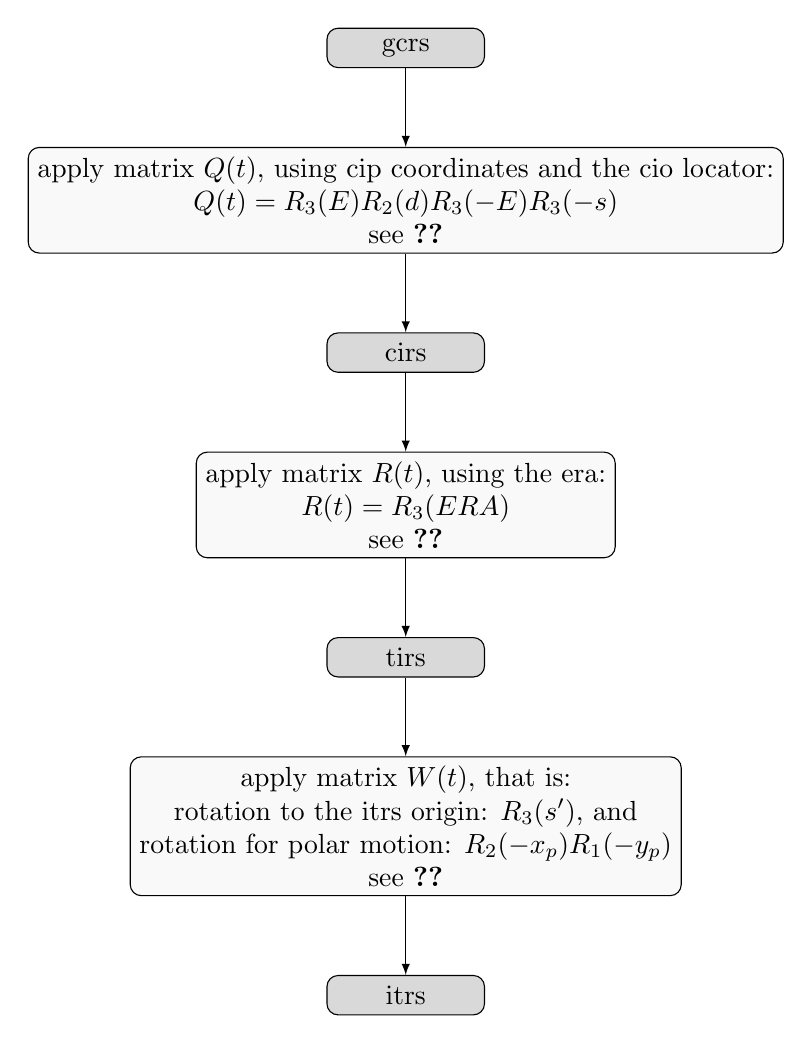
\begin{tikzpicture}[
  every node/.style = {
    draw=black, 
    rounded corners, 
    fill=gray!30,
    minimum width=2cm,
    minimum height=0.5cm,
    align=center},
  every path/.style = {
    draw,
    -latex}
  ]

  \node (gcrs) {\acrfull{gcrs}};
  
  \node[fill=gray!5] (gcrs2cirs) [below =of gcrs] {
    apply matrix \(Q(t)\), using \gls{cip} coordinates 
    and the \gls{cio} locator:\\
    \(Q(t) = R_3 (E) R_2 (d) R_3 (-E) R_3 (-s)\)\\
    see \ref{ssec:gcrs-to-cirs-via-q}
  };

  \node (cirs) [below =of gcrs2cirs] {\acrfull{cirs}};

  \node[fill=gray!5] (cirs2tirs) [below =of cirs] {
    apply matrix \(R(t)\), using the \gls{era}:\\
    \(R(t) = R_3 (ERA) \)\\
    see \ref{ssec:cirs-to-tirs-via-r}
  };
  
  \node (tirs) [below =of cirs2tirs] {\acrfull{tirs}};

  \node[fill=gray!5] (tirs2itrs) [below =of tirs] {
    apply matrix \(W(t)\), that is:\\
    rotation to the \gls{itrs} origin: \(R_3 (s')\), and \\
    rotation for polar motion: \(R_2(-x_p) R_1(-y_p)\) \\
    see \ref{ssec:tirs-to-itrs-via-w}
  };
  
  \node (itrs) [below =of tirs2itrs] {\acrfull{itrs}};

  \draw (gcrs) -- (gcrs2cirs);
  \draw (gcrs2cirs) -- (cirs);
  \draw (cirs) -- (cirs2tirs);
  \draw (cirs2tirs) -- (tirs);
  \draw (tirs) -- (tirs2itrs);
  \draw (tirs2itrs) -- (itrs);

\end{tikzpicture}

\caption{Transformation from \gls{gcrs} to \gls{itrs} using the so called ``CIO based'' procedure.}
\label{fig:bcrs-to-itrs}
\end{figure}

According to the \gls{iau} resolution (\cite{iers2010}), time coordinates for the 
\gls{bcrs} should be expressed in \gls{tcb}, whereas for \gls{gcrs}, time coordinates 
should be expressed in either \gls{tcg} or \gls{tt}. \gls{tcg} and \gls{tt} differ 
by a constant rate. The parameter \(t\) to be used in \ref{eq:tn3651}, is defined by:
\begin{equation}
  \label{eq:tn3652}
  t = (TT - \text{ 2000 January 1d 12h } TT) \text{ in days} / 36525.
\end{equation}
that is he elapsed time in Julian centuries since J2000 TT.

Two equivalent procedures can be followed to implement the relation \ref{eq:tn3651}, 
consistent with the \gls{iau} 2000/2006 resolutions; they differ by the origin 
that is adopted on the \gls{cip} equator (i.e. the equinox or the \gls{cio}) and 
are conventionaly called ``equinox based'' and ``CIO based'' respectively. The matrix 
\(W(t)\) is the same for both procedures, while \(Q(t)\) and \(R(t)\) depend on the 
corresponding origin on the \gls{cip} equator. Of the two, only the `CIO based'
procedure can be in agreement with \gls{iau} 2000 Resolution B1.8, which requires 
the use of the ``nonrotating origin'' in both the \gls{gcrs} and the \gls{itrs} as 
well as the position of the \gls{cip} in the \gls{gcrs} and in the \gls{itrs} 
(\cite{iers2010}).

\subsection{\gls{tirs} to \gls{itrs} via \(W(t)\)}
\label{ssec:tirs-to-itrs-via-w}
When applying the transformation \(W(t)\) at date \(t\), the system is transformed 
from \gls{itrs} to \gls{tirs}, which uses the \gls{cip} as its \(z\)-axis and 
the \gls{tio} as its \(x\)-axis. The formula for the transformation is
\begin{equation}
  \label{eq:tn3653}
  W(t) = R_3 (-s') R_2 (x_p ) R_1 (y_p )
\end{equation}
where \(x_p\) and \(y_p\) are the polar coordinates of the \gls{cip} in the 
\gls{itrs} (\ref{ssec:motion-of-the-cip-in-the-itrs}) and \(s'\) is the 
``TIO locator'' (\ref{ssec:position-of-the-tio-in-the-itrs}) which provides 
the position of the \gls{tio} on the equator of the \gls{cip} corresponding to 
the kinematical definition of the ``non-rotating'' origin in the \gls{itrs} 
when the \gls{cip} is moving with respect to the \gls{itrs} due to polar motion 
(\cite{iers2010}).

\subsection{\gls{cirs} to \gls{tirs} via \(R(t)\)}
\label{ssec:cirs-to-tirs-via-r}
Tthe ``CIO based'' procedure, realizes an intermediate celestial reference system 
at date \(t\) that uses the \gls{cip} as its \(z\)-axis and the \gls{cio} as its 
\(x\)-axis, called the \gls{cirs}. The matrix \(R(t)\) uses the \gls{era}, that 
is the angle between the \gls{cio} and the \gls{tio} at date \(t\) on the equator 
of the \gls{cip} (aka, the sidereal rotation of the Earth) matrix \(R(t)\), relating 
\gls{tirs} and \gls{cirs}, can be expressed as
\begin{equation}
  \label{eq:tn3655}
  R(t) = R_3 (-ERA)
\end{equation}


\subsection{\gls{gcrs} to \gls{cirs} via \(Q(t)\)}
\label{ssec:gcrs-to-cirs-via-q}
\(Q(t)\) is the matrix expressing the combined effect of nutation, precession and 
frame bias, performing the \emph{intermediate-to-celestial} transformation.
\(Q(t)\) uses the two coordinates of the \gls{cip} in the \gls{gcrs}
\begin{equation}
  \label{eq:tn3656}
  Q(t) = R_3 (-E) R_2 (-d) R_3 (E) R_3 (s)
\end{equation}
where
\begin{equation}
  \label{eq:tn3657}
  X = \sin d \cos E , \quad
  Y = \sin d \sin E , \quad
  Z = \cos d
\end{equation}
\(\left[ X  Y  Z \right]\) are the coordinates of the 
\gls{cip} in the \gls{gcrs}.
\(s\) is the ``CIO locator'' which provides the position of the \gls{cio} 
on the equator of the \gls{cip} corresponding to the kinematical definition of 
the Non-Rotating-Origin in the \gls{gcrs} when the \gls{cip} is moving with 
respect to the \gls{gcrs}, between the reference epoch and the date \(t\) due to
precession and nutation (\cite{iers2010}). Alternatively, \(Q(t)\) can be written 
as
\begin{equation}
  \label{eq:tn36510}
  Q(t) = \begin{pmatrix}
    1 - \alpha X^2 & -\alpha XY      & X \\
    -\alpha XY     & 1 - \alpha Y^2  & Y \\
    -X             &  -Y             & 1 - \alpha (X^2 + Y^2)\\
  \end{pmatrix} R_3 (s)
\end{equation}
with \(\alpha = 1 / (1 + \cos d ) \) and \(X\) and \(Y\) being the coordinates of 
the \gls{cip} in the \gls{gcrs} (\ref{ssec:coordinates-of-the-cip-in-the-gcrs}).

In contrast, the ``equinox based'' procedure \todo{Probably skip the equinox based procedure 
alltogether. Only describe the `new', CIO-based procedure} uses an intermediate celestial reference 
system that uses the \gls{cip} as its \(z\)-axis and the equinox as its \(x\)-axis, 
called the ``true equinox and equator of date system''. The matrix \(R(t)\) uses 
the \gls{gst} for Earth rotation, which transforms from the \gls{tirs} to the 
true equinox and equator of date system; \gls{gst} is the angle between the equinox 
and the \gls{tio}
\begin{equation}
  R(t) = R_3 (-GST)
\end{equation}
\(Q(t)\) uses the classical precession and nutation parameters; it can be formed 
in two ways: 
\begin{itemize}
  \item using the classical nutation angles and precession matrix, including a 
  separate rotation matrix for the frame biases, or
  \item referred directly to the \gls{gcrs} pole and origin without requiring the 
  frame bias to be applied separately, and no separate precession and nutation
  steps.
\end{itemize}

\subsection{Motion of the \gls{cip} in the \gls{itrs}}
\label{ssec:motion-of-the-cip-in-the-itrs}
The rotation of the Earth is represented by the diurnal rotation around a reference 
axis, the \gls{cip}, whose motion with respect to the \gls{irf} is represented 
by the theories of precession and nutation (\cite{esaa13}). The \gls{cip} moves 
slowly, in a \gls{trf}, is a quasi-circular path around the axis of figure (maximum 
proncipal moment of inertia). The motion of the of the \gls{trf} with respect to 
the \gls{cip} is known as \emph{polar motion} (\cite{esaa13}).

Polar motion consists of three major components: a free oscillation called 
\emph{Chandler wobble} with a period of about 435 days, an annual oscillation 
forced by the seasonal displacement of air and water masses, and an irregular 
drift, partly due to motions in the Earth's core and mantle, and partly to the 
redistribution of water mass (\cite{iersPolarmotionWs}). Unpredictable geophysical forces can 
affect the exact period and amplitude of polar motion, thus its determination 
can only be performed via observation.

The \gls{iers} publishes values for coordinates of the \gls{cip}, \(x_p\), \(y_p\).
When applied in \ref{eq:tn3653} though, additional corrections/components have 
to be applied, to account for a number of effects.

The pole coordinate parameters \(x_p \) and \(y_p\) to be used in \ref{eq:tn3653} 
(if not estimated) should be the ones published by the \gls{iers} with corrections 
for the effect of ocean tides \((\Delta x , \Delta y )_{ocean tides} \) and for the 
forced terms \((\Delta x , \Delta y )_{libration} \) with periods less than two 
days in space:
\begin{equation}
  \label{eq:tn36511}
  \begin{pmatrix}
    x_p \\
    y_p
  \end{pmatrix}
  =
  \begin{pmatrix}
    x \\
    y
  \end{pmatrix} _{IERS}
  +
  \begin{pmatrix}
  \Delta x \\
  \Delta y
  \end{pmatrix} _{ocean tides}
  +
  \begin{pmatrix}
  \Delta x \\
  \Delta y
  \end{pmatrix} _{libration}
\end{equation}

where \((x, y)_{IERS}\) are pole coordinates provided by the \gls{iers}, 
\((\Delta x, \Delta y)_{ocean tides}\) are the diurnal and semi-diurnal variations 
in pole coordinates caused by ocean tides, and \((\Delta x, \Delta y)_{libration}\) 
are the variations in pole coordinates corresponding to motions with periods 
less than two days in space that are not part of the IAU 2000 nutation model.
A detailed discussion on the variations caused by ocean tides and so-called ``libration'', 
can be found in \cite{iers2010}.

To apply the corrections, we can use one of the following schemes (after retrieving 
\gls{eop} information, e.g. from \gls{iers} Bulletin files):
\todo[color=red!40]{Is this correct? See also \cite{iers2010}, section 5.5.1. It seems that 
a call to \texttt{interp\_pole} is the same as a call to \texttt{ortho\_eop} followed 
by a call to \texttt{pmsdnut2}. The latter may give a bit better precision, but 
we first need an interpolation for the given MJD. \texttt{interp\_pole} e.g. uses 
a Lagrange interpolation algorithm using 4 data points.}

\begin{enumerate}
  \item use the function \texttt{iers2010::interp\_pole}, or
  \item use the functions \texttt{iers2010::ortho\_eop} followed by \texttt{iers2010::pmsdnut2}
\end{enumerate}

\subsection{Position of \gls{tio} in the \gls{itrs}, the ``\gls{tio} locator''}
\label{ssec:position-of-the-tio-in-the-itrs}
The \gls{tio} locator, provides the position of the \gls{tio} on the equator
of the \gls{cip}, such that there is no component of polar motion about the pole 
of rotation. This constitues a kinematical definition of the \emph{non-rotating origin} 
in the \gls{itrs}, when the \gls{cip} is moving with respect to the \gls{itrs} 
due to polar motion. The use of the \gls{tio} locator, 
\begin{displayquote}
which was neglected in the classical form prior to 1 January 2003, is
necessary to provide an exact realization of the ``instantaneous prime meridian'' 
(designated by ``TIO meridian'').
\end{displayquote} (\cite{iers2010}).

\ref{eq:tn3653} needs the \gls{tio}-locator \(s'\), which can be computed by:
\begin{equation}
  \label{eq:tn3654}
  s'(t) = \frac{1}{2} \int_{t_0}^{t} \left( 
    x_p \dot{y}_p - \dot{x}_p y_p \right) \,dt
\end{equation}
According to \cite{iers2010}, the value of \(s'\) will be less than 
\SI{0.4}{\milli\arcsecond} after one century. Using the current mean amplitudes 
for the Chandlerian and annual wobbles gives:
\begin{equation}
  \label{eq:tn36513}
  s' = -47 \text{ } \mu as \text{ } t
\end{equation}

\subsection{\acrfull{era}}
\label{ssec:earth-rotation-angle}
For the computation of \ref{eq:tn3655}, we need the \gls{era}, which is given by 
(\cite{iers2010}):
\begin{equation}
  \label{eq:tn36515}
  \begin{aligned}
  ERA(T_u ) &= 2 \pi ( UT1 \text{ Julian day fraction } \\
            &+ 0.7790572732640 + 0.00273781191135448 T_u )
  \end{aligned}
\end{equation}

where \(T_u = \text{ Julian UT1 date } - 2451545.0 \) and \( UT1 = UTC + \Delta UT1 \), 
and \(\Delta UT1 \) is provided by the \gls{iers} (if not estimated). Similarly 
to polar motion, additional components should be added to the values
published by the \gls{iers} for UT1 and LOD to account for the effects of ocean 
tides and libration.

The function \texttt{iers2010::interp\_pole} can only interpolate and apply the 
correction for the tidal terms \(\Delta UT1_{ocean\text{ }tides}\), or 
\(\Delta LOD_{ocean\text{ }tides}\) but the \(\Delta UT1_{libration}\) and 
\(\Delta LOD_{libration}\) are missing (and probably could be added, see \cite{iers2010}, 
section 5.5.3.1).

\texttt{iers2010::ortho\_eop} can be used to compute diurnal and
semi-diurnal variations in UT1 or LOD caused by ocean tides, aka 
\(\Delta UT1_{ocean\text{ }tides}\) and \(\Delta LOD_{ocean\text{ }tides}\).

\texttt{iers2010::utlibr} can be used to compute \(\Delta UT1_{libration}\) and 
\(\Delta LOD_{libration}\).

\subsection{Coordinates of the \gls{cip} in the \gls{gcrs}}
\label{ssec:coordinates-of-the-cip-in-the-gcrs}
Following the IAU 2006 precession and IAU 2000A nutation models, the parameters 
\(X\) and \(Y\) in \ref{eq:tn36510} can be computed in the microarcsecond level, 
using the formulas (\cite{iers2010}):
\begin{equation}
  \label{eq:tn36516a}
  \begin{aligned}
  X &= \SI{-0.01661700}{\arcsecond} + \SI{2004.19189800}{\arcsecond} t - \SI{0.429782900}{\arcsecond} t^2 \\
  &- \SI{0.1986183400}{\arcsecond}t^3 + \SI{0.00000757800}{\arcsecond} t^4 + \SI{0.000005928500}{\arcsecond} t^5 \\
  &+ \sum_{i} \left[ (a_{s,0})_i \sin \theta + (a_{c,0})_i \cos \theta \right] \\ 
  &+ \sum_{i} \left[ (a_{s,1})_i t \sin \theta + (a_{c,1})_i t \cos \theta \right] \\ 
  &+ \sum_{i} \left[ (a_{s,2})_i t^2 \sin \theta + (a_{c,2})_i t^2 \cos \theta \right] \\ 
  &+ \cdots \\
  \end{aligned}
\end{equation}
and
\begin{equation}
  \label{eq:tn36516b}
  \begin{aligned}
  Y &= -\SI{0.00695100}{\arcsecond} - \SI{0.02589600}{\arcsecond} t - \SI{22.407274700}{\arcsecond} t^2 \\
  &+ \SI{0.0019005900}{\arcsecond} t^3 + \SI{0.00111252600}{\arcsecond} t^4 + \SI{0.000000135800}{\arcsecond} t^5 \\
  &+ \sum_{i} \left[ (b_{s,0})_i \sin \theta     + (b_{c,0})_i \cos \theta \right] \\ 
  &+ \sum_{i} \left[ (b_{s,1})_i t \sin \theta   + (b_{c,1})_i t \cos \theta \right] \\ 
  &+ \sum_{i} \left[ (b_{s,2})_i t^2 \sin \theta + (b_{c,2})_i t^2 \cos \theta \right] \\ 
  &+ \cdots \\
  \end{aligned}
\end{equation}

where \(t\) is expressed in Julian centuries TT (\ref{eq:tn3652}) and \(\theta\) 
is a function of the fundamental lunisolar and planetary arguments. Complete 
list of coefficients for \ref{eq:tn36516a} and \ref{eq:tn36516b} is provided 
by \gls{iers}. 

Details on the position of the \gls{cip} in the \gls{gcrs} and implementation 
details, can be found in \cite{CapitaineAndWallace2006} and 
\cite{Capitaineetal2003a}.

  \chapter{Celestial Reference System and \gls{eop}}
\label{ch:celestial-rf-and-eop}

The transformation used to relate the \gls{itrs} to the \gls{gcrs} at a 
given date $t$, can be written as (\cite{iers2010}):
\begin{equation}
    \bm{r}_{GCRS} = \bm{Q}(t) \cdot \bm{R}(t) \cdot \bm{W}(t) \cdot \bm{r}_{ITRS}
    \label{eq:iers1051}
\end{equation}

where:
\begin{itemize}
    \item $\bm{Q}(t)$ is the transformation matrix arising from the
    (celestial) \textbf{polar motion} in the celestial reference system,
    \item $\bm{R}(t)$ is the transformation matrix accounting for 
    \textbf{Earth rotation} around the axis ascociated with the pole, and
    \item $\bm{W}(t)$ accounts for \textbf{polar motion}
\end{itemize}

Note that the paremeter $t$ used in \ref{eq:iers1051} is given by:
\begin{equation}
    t = \left( TT - 2000 \text{ January } 1d 12h TT \right)
    \text{ in days } / 36525
\end{equation}
where $2000 \text{ January 1d 12h TT} = \text{ Julian Date } 2451545.0 \text{ TT}$.

\ul{Here, we follow the approach compliant with the \emph{IAU 2000/2006} 
resolutions}. Hence, the quantities to be used in the matrix $\bm{Q}(t)$ in 
\ref{eq:iers1051} must be based on the \emph{IAU 2006} precession and the 
\emph{IAU 2000A} or \emph{IAU 2000B} (depending on required precision).

\section{Terrestrial to Celestial Transformation}
\label{sec:ter2cel-trans}

Currently, IERS recommends two procedures for transforming between the 
Terrestrial and Celestial reference frames, called the ``equinox based'' 
and the ``\gls{cio} based'', differing in the origin of the \gls{cip} 
equator. For further details on the ``equinox based'' transformation, see 
e.g. \cite{iers2010} and \cite{esaa13}. In the following we will discuss the 
``\gls{cio} based'' transformation, since
\begin{displayquote}
    only the CIO based
procedure can be in agreement with IAU 2000 Resolution B1.8, which requires the use of the “non-
rotating origin” in both the GCRS and the ITRS as well as the position of the CIP in the GCRS
and in the ITRS.
\end{displayquote}, \cite{iers2010}.

Each of the three rotation matrices in \ref{eq:iers1051}, represents a series 
of elementary rotations, a product of the rotation matrices $R_x(\theta)$, 
$R_y(\theta)$ and $R_z(\theta)$, with positive angle about the $x-$, $y-$ and 
$z-$axis. The position of the \gls{cip} (in both \gls{itrs} and \gls{gcrs}) is 
provided by the \gls{cip} unit vector components $x$ and $y$, called 
``coordinates'' of the \gls{cip}.

\subsection{Polar Motion Matrix $W(t)$}
\label{ssec:polar-motion-matrix}
The rotation of the Earth is represented by the diurnal rotation around a
refernce axis, called the \gls{cip}. The \gls{cip} does not coincide with 
the axis of figure of the Earth, but slowly moves (in a terrestrial reference 
frame) (\cite{esaa13}). This motion of the terrestrial reference frame 
with respect to the \gls{cip} is known as \emph{polar motion}. Note that the 
\gls{cip} is not the instantenuous axis of rotation but the axis around which the 
diurnal rotation of earth is applied (in the celestial to terrestrial 
transformation). Polar motion is typically determined from \gls{vlbi} 
observation, as except from the principal periods of 365 days (annual wobble) 
and 428 days (Chandler wobble), it is also affected by unpredictable geophysical 
forces.

According to IAU 2006 Resolution B2, the system at date $t$ as realized 
from the \gls{itrs} by applying the transformation $\bm{W}(t)$ is the 
\gls{tirs}. It uses the \gls{cip} as its $z$-axis and the \gls{tio} as 
its $x$-axis (\cite{iers2010}). This matrix gives the position of the 
terrestrial reference frame with respect to the \gls{tio}.

The $\bm{W}$ matrix can be expressed as (\cite{iers2010}):
\begin{equation}
    \bm{W}(t) = \bm{R}_z(-s') \cdot \bm{R}_y(x_p) \cdot \bm{R}(y_p)
    \label{eq:iers1053}
\end{equation},
where $s'$ is the ``\gls{tio} locator'' and $x_p$, $y_p$ are the 
``polar coordinates'' of the \gls{cip} in the \gls{itrs}. The latter values, 
if not estimated, should be the ones published by the \gls{iers}, corrected for 
the effect of ocean tides and forced terms (aka ``libration''), with periods 
less than two days in space (\cite{iers2010}), so that:
\begin{equation}
    \begin{pmatrix} x_p & y_p \end{pmatrix} = 
    \begin{pmatrix} x & y \end{pmatrix}_{IERS} + 
    \begin{pmatrix} \Delta x & \Delta y \end{pmatrix}_{ocean\text{ }tides} + 
    \begin{pmatrix} \Delta x & \Delta y \end{pmatrix}_{libration} 
\end{equation}
Handling of ocean tides and forced terms is performed similar to the \gls{iers}-
published \texttt{INTERP.F}\footnote{available from IERS at \url{https://hpiers.obspm.fr/iers/models/interp.f}} routine. 
In principle, the same result should be obtained by computing the respective 
corrections from calling \texttt{RG\_ZONT2.F}\footnote{Available from the \gls{iers} \href{https://iers-conventions.obspm.fr/}{Conventions Centre} at \url{https://iers-conventions.obspm.fr/content/chapter8/software/RG_ZONT2.F}, provided by A. Brzezinski.} 
and \texttt{PMSDNUT2.F}\footnote{Available from the \gls{iers} \href{https://iers-conventions.obspm.fr/}{Conventions Centre} at \url{https://iers-conventions.obspm.fr/content/chapter5/software/PMSDNUT2.F}, provided by A. Brzezinski.}.

\begin{itemize}
    \item The subdaily variations are not part of the polar motion values 
    reported to and distributed by the \gls{iers} and are therefore to be 
    added after interpolation (\cite{iers2010}). To perform this correction, 
    two seperate effects are taken into account,
\end{itemize}

\section{Implementation}
\label{eop-implementation}

\subsubsection{\gls{eop} Information}
\Gls{eop} information for formulating the Celestial-to-Terrestrial transformation 
matrix, is extracted from the \gls{iers} \texttt{C04} files (\cite{Bizouard2019}).
These files contain tabulated \gls{eop} values at 0\textsuperscript{h} \gls{utc}. 

These files can be read into an \texttt{dso::EopLookUpTable} instance, using 
the function \texttt{dso::parse\_iers\_C04}.

According to \cite{Bradley2016850}:
\begin{displayquote}
    Prior to the interpolation of DUT1 and LOD, the tabulated values
    should be smoothed through regularization to enhance the
    interpolation accuracy. Regularization is the removal of
    zonal tidal variations with frequencies ranging from 5 days
    to 18.6 years.
\end{displayquote}


\begin{figure}
\centering
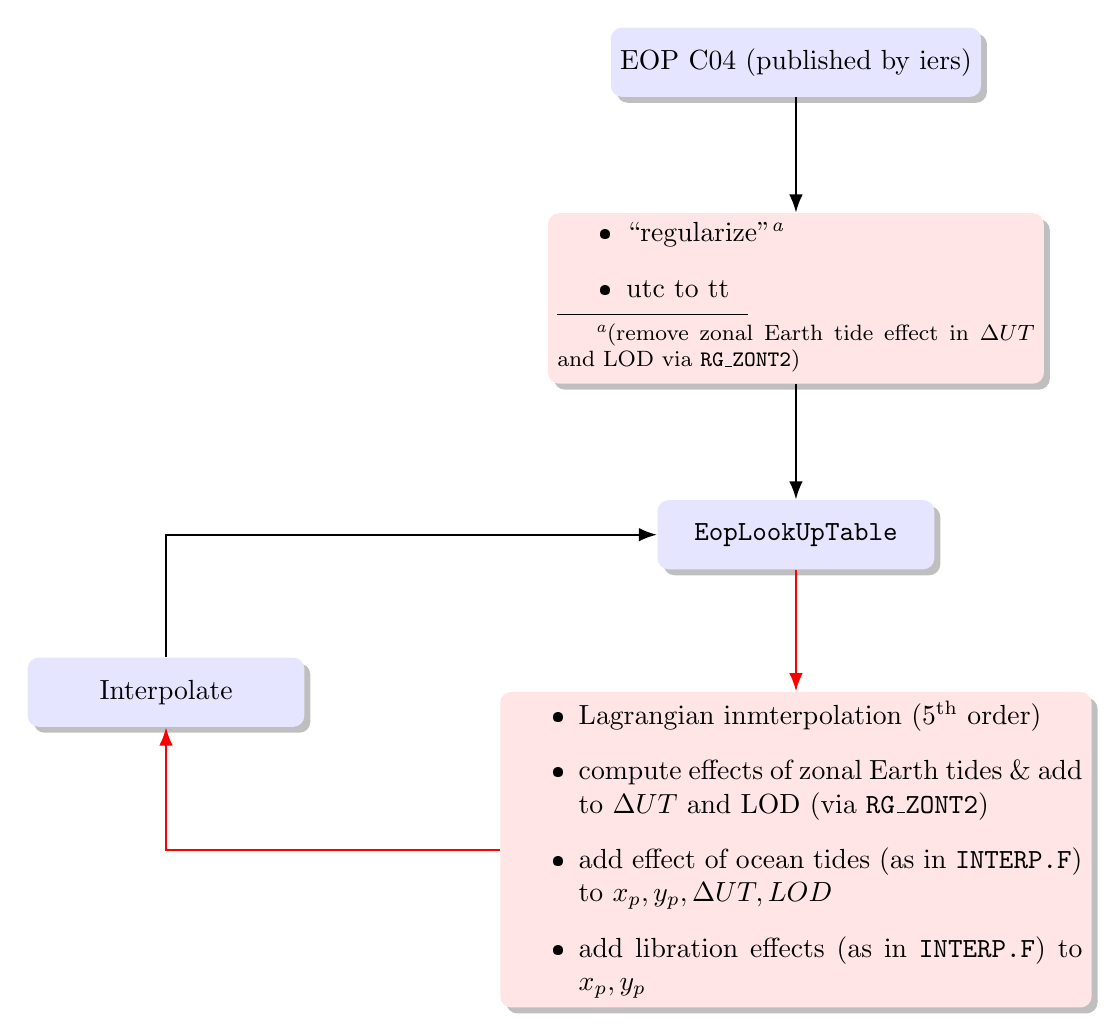
\begin{tikzpicture}
	\node (A) at (0,0) 
		[minimum height=2.5em, minimum width=10em, fill=blue!10,rounded corners, drop shadow] 
		{EOP C04 (published by \gls{iers})};
	
	\node (AtB) at (0,-3) 
		[minimum height=2.5em, minimum width=10em, fill=red!10,rounded corners, drop shadow]
		{\begin{minipage}{.5\textwidth}\begin{itemize}
		\item ``regularize''\footnote{(remove zonal Earth tide effect in $\Delta UT$ and LOD via \texttt{RG\_ZONT2})}
		\item \gls{utc} to \gls{tt}
		\end{itemize}\end{minipage}};
		
	\node (B) at (0,-6.0) 
		[minimum height=2.5em, minimum width=10em, fill=blue!10,rounded corners, drop shadow] 
		{\texttt{EopLookUpTable}};

	\node (BtI) at (0,-10) 
		[minimum height=2.5em, minimum width=10em, fill=red!10,rounded corners, drop shadow]
		{\begin{minipage}{.6\textwidth}\begin{itemize}
		\item Lagrangian inmterpolation (5\textsuperscript{th} order)
		\item compute effects of zonal Earth tides \& add to $\Delta UT$ and LOD (via \texttt{RG\_ZONT2})
		\item add effect of ocean tides (as in \texttt{INTERP.F}) to $x_p, y_p, \Delta UT, LOD$
		\item add libration effects (as in \texttt{INTERP.F}) to $x_p, y_p$
		\end{itemize}\end{minipage}};
	
	\node (I) at (-8,-8)
		[minimum height=2.5em, minimum width=10em, fill=blue!10,rounded corners, drop shadow]
		{Interpolate};

	\draw[-Latex,thick] (A.south) -- (AtB.north);
	\draw[-Latex,thick] (AtB.south) -- (B.north);
	\draw[-Latex,thick] (I.north) |- (B.west);
	\draw[-Latex,red,thick] (B.south) -| (BtI.north);
	\draw[-Latex,red,thick] (BtI.west) -| (I.south);
	%\draw[->] (A)--(B) node[midway]{Remove effects of zonal Earth tides on $\Delta$UT and LOD (\texttt{rg\_zont2})}; 
\end{tikzpicture}

\caption{Extracting \gls{eop} information from \gls{iers} \texttt{C04} data files.}
\label{fig:handling-eop}
\end{figure}

  \chapter{Tides}
\label{ch:tides}

\section{Solid Earth Tides}
\label{sec:solid-earth-tides}

\subsubsection{Solid Earth Tide Effect on Geopotential}
\label{sssec:solid-earth-tide-geopotential}
The changes induced by the solid Earth tides in the free space potential are 
most conveniently modeled as variations in the standard geopotential 
coefficients $C_{nm}$ and $S_{nm}$, labled $\Delta C_{nm}$ and $\Delta S_{nm}$ 
respectively, expressible in terms of the Love number $\lovek$. The effects of 
ellipticity and of the Coriolis force due to Earth rotation on tidal 
deformations necessitate the use of three $\lovek$ parameters, $\lovek ^{(0)}_{nm}$ 
and $\lovek ^{(\pm)}_{nm}$ (except for $n = 2$) to characterize the
changes produced in the free space potential by tides of spherical harmonic 
degree and order $(nm)$, whereas only two parameters are needed for $n = 2$ 
because $\lovek ^{(-)}_{2m} = 0$ due to mass conservation (\cite{iers2010}).

Solid Earth tides within the diurnal tidal band (for which $(n,m) = (2,1)$) are 
not wholly due to the direct action of the \gls{tgp} on the solid Earth; they 
include the deformations (and associated geopotential changes) arising from 
other effects of the \gls{tgp}, namely, ocean tides and wobbles of the mantle 
and the core regions (\cite{iers2010}).

The computation of the tidal contributions to the geopotential coefficients is 
most efficiently done by a three-step procedure:
\begin{itemize}
  \item In Step 1, the $(2m)$ part of the tidal potential is evaluated in the 
   time domain for each $m$ using lunar and solar ephemerides, and the 
   corresponding changes $\Delta \bar{C}_{2m}$ and $\Delta \bar{S}_{2m}$ are 
   computed using frequency independent nominal values $\lovek _{2m}$ for the 
   respective $\lovek ^{(0)}_{2m}$. The contributions of the degree 3 tides to
   $\bar{C}_{3m}$ and $\bar{S}_{3m}$ through $\lovek ^{(0)}_{3m}$ and also of 
   those of the degree 2 tides to $\bar{C}_{4m}$ and $\bar{S}_{4m}$ though 
   $\lovek ^{(+)}_{2m}$ may be computed by a similar procedure.

   With frequency-independent values $\lovek _{nm}$, changes induced by the 
   $(nm)$ part of the \gls{tgp} in the \emph{normalized} geopotentials 
   coefficients of the same degree and order $(nm)$, are given in the time 
   domain by (\cite{iers2010}):
   \begin{equation}
    \Delta \bar{C}_{nm} - \iim \Delta \bar{S}_{nm} = \frac{\lovek _{nm}}{2n+1}
      \sum^{3}_{j=2} \frac{GM_j}{GM_\Earth} \left( \frac{R_e}{r_j} \right) ^{n+1} 
      \bar{P}_{nm} \left( \sin \Phi _j \right) e^{-\iim m \lambda _j}
      \label{eq:iers1066}
   \end{equation}
    where:
    \begin{description}
      \item $\lovek _{nm}$\footnote{Tables of relevant Love numbers are listed 
        in \cite{iers2010}, Table 6.3.} is the nominal Love number for degree 
        $n$ and order $m$, 
      \item $R_e$ and $GM_{\Earth}$ are the equatorial radius and the 
        gravitational parameter of the Earth,
      \item $GM_j$ is the gravitational parameter of the Moon and Sun, for 
        $j=2$ and $j=3$ respectively,
      \item $\Phi _j$ is the body-fixed geocentric latitude of the Moon and 
        Sun ($j$ indexes as above), and
      \item $\lambda _j$ is the body-fixed (east) logitude of the Moon and 
        Sun ($j$ indexes as above)
    \end{description}

    For $n=4$, formula \ref{eq:iers1066} becomes (\cite{iers2010}):
    \begin{equation}
    \Delta \bar{C}_{4m} - \iim \Delta \bar{S}_{4m} = \frac{\lovek _{nm}}{5}
      \sum^{3}_{j=2} \frac{GM_j}{GM_\Earth} \left( \frac{R_e}{r_j} \right) ^{3} 
      \bar{P}_{2m} \left( \sin \Phi _j \right) e^{-\iim m \lambda _j} \text{ for } m=0,1,2
      \label{eq:iers1067}
    \end{equation}
    to account for the changes in the degree 4 coefficients produced by the 
    degree 2 tides.

    In Step 1, we compute corrections for 
    \begin{equation}
      \Delta \bar{C}_{nm}, \Delta \bar{S}_{nm} \text{ for }
        \begin{cases}
          n=2 & m=0,1,2 \\
          n=3 & m=0,1,2,3 \\
          n=4 & m=0,1,2\\
        \end{cases}
    \end{equation} 

  \item in Step 2 we compute corrections for the deviations of the 
  $\lovek ^{(0)}_{21}$ from the constant nominal value $\lovek _{21}$ 
  assumed (for this band) in the first step. Similar corrections need to be 
  applied to a few of the constituents of the other two bands also.
\end{itemize}

Steps 1 and 2 can be used to compute the total tidal contribution, including 
the time independent (permanent) contribution to the geopotential coefficient 
$\bar{C}_{20}$, which is adequate for a ``conventional tide free'' model. 
When using a ``zero tide'' model, this permanent part should not be counted 
twice.

\subsubsection{Solid Earth Tide Effect on Reference Points}
\label{sssec:solid-earth-tide-reference-points}

Site displacements caused by tides of spherical harmonic degree and order $(nm)$ 
are characterized by the Love number $loveh _{nm}$ and the Shida number $\lovel _{nm}$. 
The effective values of these numbers depend on station latitude and tidal 
frequency (\cite{WahrEtAl1981}).

Computation of the variations of station coordinates due to solid Earth tides, 
like that of geopotential variations, is done most efficiently by the use of a 
two-step procedure (\cite{iers2010}). The evaluations in the first step use 
the expression in the time domain for the full degree 2 tidal potential or for 
the parts that pertain to particular bands $(m = 0, 1, \text{ or } 2)$. Nominal 
values common to all the tidal constituents involved in the potential and to 
all stations are used for the \emph{Love} and \emph{Shida} numbers $\loveh _{2m}$ 
and $\lovel _{2m}$ in this step. Along with expressions for the dominant 
contributions from $\loveh ^{(0)}$ and $\lovel ^{(0)}$ to the tidal displacements,
relatively small contributions from some of the other parameters are included 
in Step 1 for reasons of computational efficiency. The displacements caused by 
the degree 3 tides are also computed in the first step, using constant values 
for $\loveh _3$ and $\lovel _3$ (\cite{iers2010}).

Corrections to the results of the first step are needed to take account of the 
frequency-dependent deviations of the \emph{Love} and \emph{Shida} numbers from 
their respective nominal values, and also to compute the out-of-phase 
contributions from the zonal tides. Computations of these corrections constitute 
Step 2. The total displacement due to the tidal potential is the sum of the 
displacements computed in Steps 1 and 2 (\cite{IERS2010}).

A short overview of the relevant computation formulas follows. More information 
can be found in \cite{iers2010} and references therein.

\textbf{\ul{In-phase displacement due to degree 2 tides, with nominal values for 
$\loveh ^{(0)}_{2m}$ and $\lovel ^{(0)}_{2m}$}}.\\
The displacement vector of the station due to the degree 2 tides is given by 
(\cite{iers2010}):
\begin{equation}
  \Delta \bm{r} = \sum ^{3}_{2} \frac{GM_j R^4_{\Earth}}{GM_{\Earth}R^3_j}
    \biggl\{ \loveh _2 \hat{r} \left( \frac{3 (\hat{R}_j \cdot \hat{r})^2 -1}{2} \right) 
      + 3 \lovel _2 (\hat{R}_j \cdot \hat{r}) \left[ \hat{R}_j - (\hat{R}_j \cdot \hat{r}) \hat{r} \right] 
    \biggl\}
    \label{eq:iers105}
\end{equation}
where \begin{description}
  \item $GM_j$ is the gravitational parameter for the Moon ($j=2$) and Sun ($j=3$),
  \item $GM_{\Earth}$ is the gravitational parameter for the Earth,
  \item $\hat{R}_j, R_j$ is unit vector from the geocenter to Moon or Sun and 
    the magnitude of that vector,
  \item $R_{\Earth}$ is the Earth’s equatorial radius,
  \item $\hat{r}, r$ is the unit vector from the geocenter to the station and 
    the magnitude of that vector,
  \item $\loveh _2$ and $\lovel _2$ are the \emph{Lova} and \emph{Shida} numbers 
    of degree 2
\end{description}

\textbf{\ul{In-phase displacement due to degree 3 tides, with nominal values for
$\loveh ^{(0)}_{2m}$ and $\lovel ^{(0)}_{2m}$}}.\\

Only the Moon’s contribution needs to be computed, the term due to the Sun being
negligible. The transverse part of the displacement does not exceed \SI{0.2}{\mm}, 
but the radial displacement can reach \SI{1.7}{\mm} (\cite{iers2010}).

The displacement vector due to these tides is then given by (\cite{iers2010}):
\begin{equation}
  \begin{aligned}
  \Delta \bm{r} = \frac{GM_{Moon} R^5_{\Earth}}{GM_{\Earth}R^4_{Moon}} &
    \biggl\{ \loveh _3 \hat{r} \left( \frac{5}{2} (\hat{R}_{Moon} \cdot \hat{r})^3) -\frac{3}{2} (\hat{R}_{Moon} \cdot \hat{r}) \right) \\
      & + \lovel _2 \left( \frac{15}{2}(\hat{R}_{Moon} \cdot \hat{r})^2 - \frac{3}{2}\right) \left[ \hat{R}_{Moon} - (\hat{R}_{Moon} \cdot \hat{r}) \hat{r} \right] 
    \biggl\}
    \end{aligned}
    \label{eq:iers106}
\end{equation}

/* Add formulas here from Section 7.1.1 Effects of the solid Earth tides */

\gls{IERS} publishes a FORTRAN program to perform the Step 1 and Step 2 computations 
called \texttt{DEHANTTIDEINEL.F}\footnote{Available from the \gls{iers} \href{https://iers-conventions.obspm.fr/}{Conventions Centre} at \url{https://iers-conventions.obspm.fr/content/chapter7/software/dehanttideinel}}.

\section{Secular polar motion and the pole tide}
\label{sec:pole-tides}

Changes in the direction of the Earth's rotation axis with respect to locations 
on the Earth's surface cause local deformations (\cite{Desai2002}) that result in 
variations in station coordinates up to a few centimeters.

To perform the corrections of the induced effect, we have to compute the so-called 
``secular pole'' (\cite{iers2010}, Sec. 7.1.4). Its coordinates, designated by 
$(x_s, y_s)$ are computed according to (\cite{iers2010}):

\begin{equation}
  \begin{aligned}
    x_s &= 55.0 + 1.677 \cdot (t-2000) \text{ in } \si{\milli\larcsecond} \\
    y_s &=  320.5 + 3.460 \cdot (t-2000) \text{ in } \si{\milli\larcsecond}
  \end{aligned}
\end{equation}
where $t$ is the date in years of 365.25 days.

  %\chapter{DORIS}
  %\label{ch:doris}
  \section{DORIS RINEX}\label{sec:doris-rinex}

\subsection{General Format  Description}
The DORIS RINEX format consists of one ASCII file containing both space based 
and meteorological data collected at DORIS stations and relayed by satellites.

DORIS RINEX format bears close resemblance\footnote{The format specifications are 
actually close to identical.} to the GNSS RINEX Version 3 (\cite{RINEX305}).
Data files consist of a header section and a data section. The first contains 
global information for the entire file, while the latter contains the actual 
observations and a date tag, keeping strict chronological order.

DORIS is basically running on its own proper time which is constantly linked 
to \gls{tai}. Time tags are given in instrument time, clock offsets are given 
between instrument time and \gls{tai}.

Observation types recorded in the DORIS RINEX files are the given in table

\begin{table}[h!]
\centering
\begin{tabular}{|c c c|}
\hline
Descriptor & Observation Type & Units \\
\hline
\texttt{L} & carrier phase observation & cycles \\
\texttt{C} & pseudo-range observation & \si{\metre}\\
\texttt{W} & power level received at each frequency & \si{\dBm} \\
\texttt{F} & relative frequency offset of the receiver’s oscillator $\frac{f-f_0}{f_0}$ & $10^{-11}$ \\
\texttt{P} & ground pressure at the station & 100 \si{\pascal} (\si{\milli\bar}) \\
\texttt{T} & ground temperature at the station & \si{\degreeCelsius} \\
\texttt{H} & ground humidity at the station & \si{\percent} \\
\hline
\end{tabular}
\caption{DORIS RINEX observation types}
\label{table:doris-rinex-observation-types}
\end{table}

\subsection{Receiver Clock Offsets}

DORIS RINEX contain a ``receiver clock offset'' \(\tau_{r_{offset}}\) (as an 
optional field) at the header record of every epoch. E.g. the line
\begin{verbatim}
    ...
    > 2020 01 01 00 00 35.099949800  0  1       -3.248177132 0
    ...
\end{verbatim}
records a receiver clock offset of \SI{35.099949800}{\second} followed by the 
receiver clock offset flag, which in this case is \num{0}. In such record 
lines, the date (given as YYYY MM DD HH MM SS.) is given in the on-board time 
scale (aka proper time of the receiver) and the conversion to the \gls{tai} 
time scale is obtained by adding the receiver clock offset.

\textit{Depending on the version of the RINEX file, this offset can have been either 
computed by the DORIS-DIODE navigator, or through a post-fit processing using PANDOR. 
In the first case, the file ends with ``.001'' whereas in the second with ``.010''. 
More information on the computation of (\(\tau_{r_{offset}}\) are provided in 
\cite{lemoine-2016}.}

\subsection{Types of DORIS measurements}
\label{ssec:types-of-doris-measurements}

\subsubsection{Relative Frequency Offset}
\label{sssec:relative-frequency-offset}

DORIS RINEX files (usually) contain a measurement type labeled ``F'' (should be 
recorded in the field \verb|SYS/#/OBS TYPES| at the RINEX header). This measurement 
type is provided for every epoch and is a measure of the relative frequency 
offset of the receiver's oscillator (aka \(\frac{f-f_0}{f_0}\) \num{10e-11}).
Example (rinex header):

\begin{adjustbox}{max width=\linewidth , fbox=0.5pt}
\begin{BVerbatim}
        0.9768        0.0001        0.0011                  CENTER OF MASS: XYZ
D   10  L1  L2  C1  C2  W1  W2   F   P   T   H              SYS / # / OBS TYPES
  2018    01    01    00    00   28.8526816     DOR         TIME OF FIRST OBS
...
                                                            END OF HEADER
> 2018 01 01 00 00 32.589951370  0  3       -3.737269708 0
D01  -2104936.480    -1241282.301   131837622.17412 131837685.14912      -124.650 7
         -114.150 7      5643.911        1025.000 1         6.000 1        85.000 1
D02  -1063469.796    -1862572.573   136575183.93813 136575216.89713      -118.350 7
         -109.250 7      5643.911        1014.000 0       -18.800 0        73.000 0
D03   -826480.354    -2642364.157   148404267.53014 148404098.13114      -115.200 7
         -104.700 7      5643.911         934.000 0       -21.500 0        72.000 0
...                                                            
\end{BVerbatim}
\end{adjustbox}

  \chapter{DORIS Ground Segment}
\label{ch:doris-ground-segment}

\tikzset{cross/.style={cross out, draw=red, minimum size=2*(#1-\pgflinewidth), inner sep=0pt, outer sep=0pt},
%default radius will be 1pt. 
cross/.default={1pt}}

\section{Geometry of Ground Antennae}
DORIS observations are referred to the electronic reference point (RP) of the antenna, 
the points where the DORIS observations  are  acquired.  As  that  electronic  point 
(\SI{2}{\GHz} center of phase for DORIS) is virtual and as for example it may change 
while using another type of antenna data referring to that electronic point are of no 
use for geophysical studies. So, observations must be referred to the conventional RP 
which is defined according to the geometry of the antenna. Therefore, one has also to 
account for the distance between the electronic RP and the conventional RP of the antenna (\cite{TOURAIN2016}). 
The ability to get accurate DORIS data relies for one part on the capability of providing 
accurate models to connect the  electronic RP (or electronic phase center) and the conventional 
RP, as well as, phase center variations (\gls{pcv}s) as a function of the elevation angle and azimuth.

The type of antenna is identified by the 4\textsubscript{th} character of the beacon 
mnemonic: letter ``A'' for the Alcatel type; letter ``B'' or letter ``C'' for the 
Starec B or C type.  That is, in the DORIS RINEX field ``STATION REFERENCE'', the 
last character of the second column (aka ``4-character station code''), defines the 
ground beacon antenna type; example:

\begin{adjustbox}{max width=\linewidth , fbox=0.5pt}
\begin{BVerbatim}[commandchars=\\\{\}]
    51                                                      # OF STATIONS       
D01  BEM\textcolor{red}{B} BELGRANO                      66018S002  3   0    STATION REFERENCE   
D02  ADH\textcolor{red}{C} TERRE ADELIE                  91501S005  3   0    STATION REFERENCE   
D03  SYQ\textcolor{red}{B} SYOWA                         66006S005  3   0    STATION REFERENCE   
D04  CRQ\textcolor{red}{C} CROZET                        91301S004  4   0    STATION REFERENCE   
D05  DIO\textcolor{red}{B} DIONYSOS                      12602S012  3   0    STATION REFERENCE
\end{BVerbatim}
\end{adjustbox}

\begin{table}[h!]
    \centering
    \begin{tabular}{|c | c | c | c | c|}
        \hline
        Zenith Distance & \multicolumn{2}{c}{ALCATEL (dBi)} & \multicolumn{2}{c|}{STAREC (dBi)} \\
                        & \SI{401.25}{\mega\hertz} & \SI{2036.25}{\mega\hertz} &  \SI{401.25}{\mega\hertz} & \SI{2036.25}{\mega\hertz}\\
        \hline
        \ang{0}&3.2&2.1&3.5&0 \\
        \ang{10}&3.5&2.6&3.6&0.4\\
        \ang{20}&4&2&3.7&0.5\\
        \ang{30}&4.4&4&3.8&1.5\\
        \ang{40}&4.6&4.4&3.7&3.2\\
        \ang{50}&4.2&4.6&3.2&3.9\\
        \ang{60}&2.7&2.7&2.5&4\\
        \ang{70}&0.6&-0.1&1&3.2\\
        \ang{80}&-2.7&-3.3&-1.3&0.2\\
        \ang{90}&-6&-7&-4.2&-5.6\\
        \hline
    \end{tabular}
    \caption{DORIS ground antennae gains, \cite{DORISGSM}.}
    \label{table:antenna-gains}
\end{table}

\subsection{Phase Center Offsets}

Depending on the antenna type, appropriate \gls{pco}s need to be applied to 
the observed quantities for the reduction of the observation vector to the Reference Point 
(from the respective ``virtual'' phase center) of the antenna. When a linear combination 
of the observed quantities is used, a respective \gls{pco} needs to be computed and 
applied. E.g., for the case of the Ionospheric-free linear combination, the respective 
\gls{pco} is:
\begin{equation}
    \vec{r}_{2GHz,iono-free} = \frac{\vec{r}_{400MHz,2GHz}}{\gamma - 1}
\end{equation}

where $\vec{r}_{2GHz,iono-free}$ is the vector from the \SI{2}{\GHz} phase
center to the iono-free phase center and $\vec{r}_{400MHz,2GHz}$ is
the vector from the \SI{400}{MHz} to the \SI{2}{\GHz} phase center.

\begin{table}[h!]
    \centering
    \begin{tabular}{|c|c|c|}
        \hline
        Antenna Type & ALCATEL & STAREC-B \& STAREC-C \\
        \hline
        $\Delta h$ in \si{\mm} for \SI{2}{\GHz} & \SI{510}{\mm} & \SI{487}{\mm}\\
        $\Delta h$ in \si{\mm} for \SI{400}{\MHz} & \SI{335}{\mm} & \SI{0}{\mm}\\
        \hline
    \end{tabular}
    \caption{DORIS ground antennae Phase Center Offsets, \cite{DORISGSM}.}
    \label{table:antenna-pco}
\end{table}

\subsection{DORIS ALCATEL Antenna}

\begin{figure}
\centering
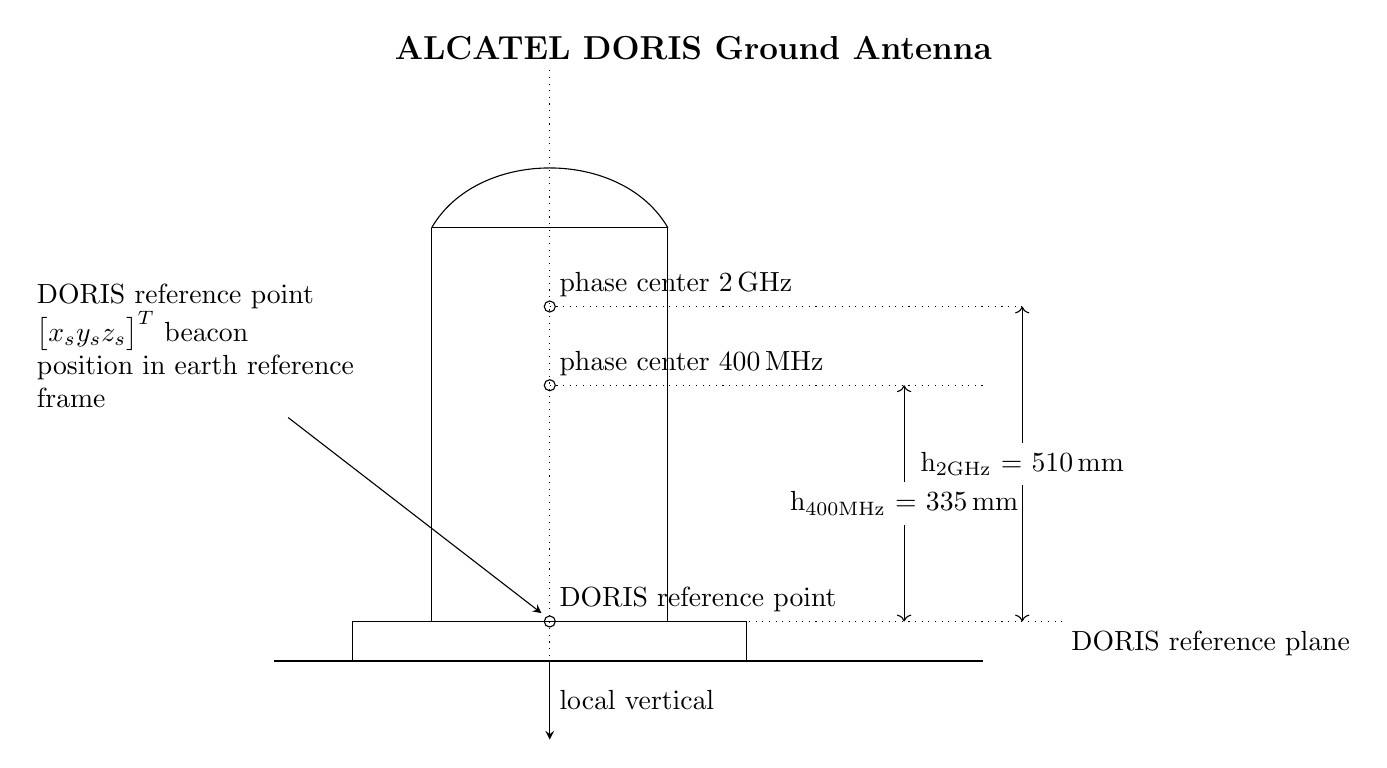
\begin{tikzpicture}
    \draw (2,-2) -- (2,-7); %% left vertical
    \coordinate (LT) at (2,-2);
    \draw (5,-2) -- (5,-7); %% right vertical
    \coordinate (RT) at (5,-2);
    \coordinate (L2PC) at (3.5, -4.0);
    \coordinate (L1PC) at (3.5, -3.0);
    \coordinate (BRP) at (3.5, -7.0);
    \draw (LT) to[out=60, in=120] (RT); %% dome
    \draw (LT) to (RT); %% top horizontal (under dome)
    \draw (1,-7) -- (6,-7); %% reference plain
    \draw (1, -7) -- (1, -7.5); %% left minor vertical
    \draw (6, -7) -- (6, -7.5); %% right minor vertical
    \draw [line width=0.25mm] (0,-7.5) -- (9,-7.5); %% ground
    \draw [-stealth] (3.5,-7.5) --node[anchor=west]{local vertical} (3.5, -8.5); %% local vertical to ground
    \draw [dotted] (3.5, 0) -- (3.5, -7.5); %% local vertical from dome
    
    \draw (L1PC) circle (2pt) node[anchor=south west]{phase center \SI{2}{\GHz}}; %% 2GHz pc
    \draw (L1PC) node[cross=3pt, rotate=0] {}; %% 2GHz cross
    \draw [dotted] (L1PC) -- (9.5, -3.0); %% horizontal from 2GHz PC
    \path (9.5, -7.0) -- node[](hl1){h\textsubscript{2GHz} = \SI{510}{\mm}} (9.5, -3.0);
    \draw [<-] (9.5, -7.0)--(hl1); \draw [->] (hl1)--(9.5, -3.0);
    
    \draw (L2PC) circle (2pt) node[anchor=south west]{phase center \SI{400}{\MHz}}; %% 400 MHz pc
    \draw (L2PC) node[cross=3pt, rotate=0] {}; %% 400MHz cross
    \draw [dotted] (L2PC) -- (9, -4.0); %% horizontal from 400MHz PC
    \path (8, -7.0) -- node[](hl2){h\textsubscript{400MHz} = \SI{335}{\mm}} (8, -4.0);
    \draw [<-] (8, -7.0)--(hl2); \draw[->] (hl2)--(8, -4.0);
    
    \draw (BRP) circle (2pt) node[anchor=south west]{DORIS reference point}; %% reference point
    \draw (BRP) node[cross=3pt, rotate=0] {}; %% RP cross
    \draw [dotted] (BRP) -- (10, -7.0); %% horizontal from RP
    \draw (10, -7) node[anchor=north west]{DORIS reference plane};
    
    \node[rectangle, align=left] (rptext) at (-1,-3.5) {DORIS reference point \\ \(\begin{bmatrix} x_s y_s z_s \end{bmatrix}^{T} \) beacon \\position in earth reference \\frame};
    \draw [-stealth] (rptext) to ($(BRP)-(3pt,-3pt)$);
    \node[above,font=\large\bfseries] at (current bounding box.north) {ALCATEL DORIS Ground Antenna};
\end{tikzpicture}

\caption{Geometry of Alcatel DORIS Ground Antenna/Beacon}
\label{fig:alcatel-antenna}
\end{figure}


\subsection{DORIS STAREC Antenna}
STAREC antennae B and C are identical in terms of design and specification, the
difference is about the error budget in phase center position. For STAREC-C,
manufacturing process and error budget have been improved \cite{DORISGSM}.

According to \cite{TOURAIN2016}, in order to check the consistency of the theoretical 
characteristics of this type of antennae, a measurement campaign was performedby 
the CNES at the Compact Antenna Test Range (CATR). The CATR is a dedicated facility 
consisting ofan anechoic chamber equipped with several specific devices 
allowing significant measurement for satellite characterization.

As a result of the campaign, a phase law was established by averaging the estimated 
phase law values obtained during the CATR characterization. The resulting couple phase 
center position–phase law correction was provided to the  DORIS  users  through  a  
text  file  in  \gls{antex} (\cite{ANTEXv14}) format, available on the IDS website
\url{ftp://ftp.ids-doris.org/pub/ids/stations/doris_phase_law_antex_starec.txt}.

STAREC antennae B and C are identical in terms of design and specification, the
difference is about the error budget in phase center position. For STAREC C,
manufacturing process and error budget have been improved (\cite{DORISGSM}).

\begin{figure}
\centering
\tikzset{cross/.style={cross out, draw=red, minimum size=2*(#1-\pgflinewidth), inner sep=0pt, outer sep=0pt},
%default radius will be 1pt. 
cross/.default={1pt}}

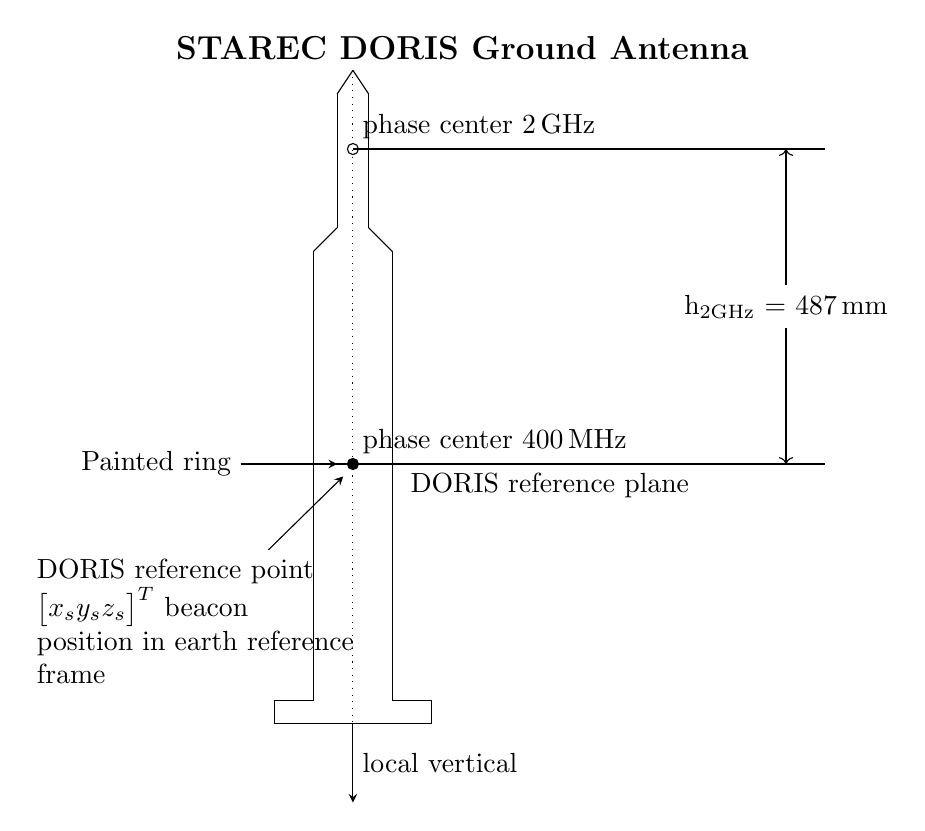
\begin{tikzpicture}
    \coordinate (top) at (4,-1);
    \coordinate (tl) at (3.8, -1.3);
    \coordinate (tr) at (4.2, -1.3);
    \coordinate (blt) at (3.8, -3.0);
    \coordinate (brt) at (4.2, -3.0);
    \coordinate (blb) at (3.5, -3.3);
    \coordinate (brb) at (4.5, -3.3);
    \draw (top) to (tl);
    \draw (tl) to (blt);
    \draw (blt) to (blb);
    \draw (top) to (tr);
    \draw (tr) to (brt);
    \draw (brt) to (brb);
    \draw (blb) to (3.5, -9);
    \draw (brb) to (4.5, -9);
    \draw (3.5, -9) to (3.0, -9);
    \draw (3.0, -9) to (3.0, -9.3);
    \draw (4.5, -9) to (5.0, -9);
    \draw (5.0, -9) to (5.0, -9.3);
    \draw (3.0, -9.3) to (5.0, -9.3);

    \draw [dotted] (top) -- (4.0, -9.3); %% local vertical from top
    \draw [-stealth] (4.0, -9.3) -- node[anchor=west]{local vertical} (4.0, -10.3); %% local vertical arrow

    \coordinate (l1pc) at (4, -2.0);
    \draw (l1pc) circle (2pt) node[anchor=south west]{phase center \SI{2}{\GHz}}; %% 2GHz pc
    \draw (l1pc) node[cross=3pt, rotate=0] {}; %% 2GHz cross
    \draw (l1pc) to (10, -2.0);
    
    \coordinate (l2pc) at (4, -6.0);
    \draw [fill=black] (l2pc) circle (2pt) node[anchor=south west]{phase center \SI{400}{\MHz}}; %% 400MHz pc
    \draw (l2pc) node[cross=3pt, rotate=0] {}; %% 400MHz cross
    \draw ($(l2pc)-(1.0,0.0)$) -- node[below]{DORIS reference plane} (10, -6.0);
    \node (prt) at ($(l2pc)-(2.5,0.0)$) {Painted ring}; 
    \draw [-stealth] (prt) to ($(l2pc)-(0.2,0.0)$);

    \path ($(l1pc)+(5.5, 0.0)$) -- node[](h2g){h\textsubscript{2GHz} = \SI{487}{\mm}} ($(l2pc)+(5.5, 0.0)$);
    \draw [<-] ($(l1pc)+(5.5, 0.0)$) -- (h2g); 
    \draw [->] (h2g) -- ($(l2pc)+(5.5, 0.0)$);

    \node[rectangle, align=left] (rptext) at ($(l2pc)-(2.0,2.0)$) {DORIS reference point \\ \(\begin{bmatrix} x_s y_s z_s \end{bmatrix}^{T} \) beacon \\position in earth reference \\frame};
    \draw [-stealth] (rptext) to ($(l2pc)-(3.5pt,4.5pt)$);

    \node[above,font=\large\bfseries] at (current bounding box.north) {STAREC DORIS Ground Antenna};
\end{tikzpicture}

\caption{Geometry of Alcatel STAREC Ground Antenna/Beacon}
\label{fig:starec-antenna}
\end{figure}

\section{Phase Law}

\begin{tikzpicture}
\pgfplotstableread{tikz/phase_law.dat}{\table}
\begin{groupplot}[
  group style={
        group name= phase-law-plots,
        group size=1 by 2,
        xlabels at=edge bottom,
        xticklabels at=edge bottom,
        vertical sep=8pt,
    },
  %title={\texttt{patch type=quadratic spline}},
  xmin=0, xmax=90,
  ymin=-5, ymax=25,
  xtick distance = 5,
  ytick distance = 5,
  grid = both,
  minor tick num = 1,
  major grid style = {lightgray},
  minor grid style = {lightgray!25},
  width = \textwidth,
  height = 0.4\textwidth,
  xlabel = {Zenith angle ($^{\circ}$)},
]
\nextgroupplot[]
\addlegendimage{empty legend};
\addplot[blue, mark = *] table [x = {Zenith}, y = {Alcatel_1}] {\table};
\addlegendentry{\texttt{Alcatel Antenna}}[15 pt];
\coordinate (top) at (rel axis cs:0,1);% coordinate at top of the first plot

\nextgroupplot[]
\addlegendimage{empty legend};
\addplot[blue, mark = *] table [x = {Zenith}, y = {Starec_1}] {\table};
\addlegendentry{\texttt{Starec Antenna}}[15 pt];
\coordinate (bot) at (rel axis cs:0,0);% coordinate at bottom of the last plot

\end{groupplot}

\path (top-|current bounding box.west)-- node[anchor=south,rotate=90] 
  {Phase Correction for 2GHz ($mm$)} (bot-|current bounding box.west);

\path (top-|current bounding box.west) --
  node[anchor=south]{\textbf{DORIS Antennae Phase Law}} 
  (top-|current bounding box.east);
%\node (title) at ($(group c1r1.center)!0.5!(group c2r1.center)+(0,2cm)$) 
%  {DORIS Antenae Phase Law};
\end{tikzpicture}

%\begin{figure}
%\begin{subfigure}{0.45\textwidth}
%  \centering
%  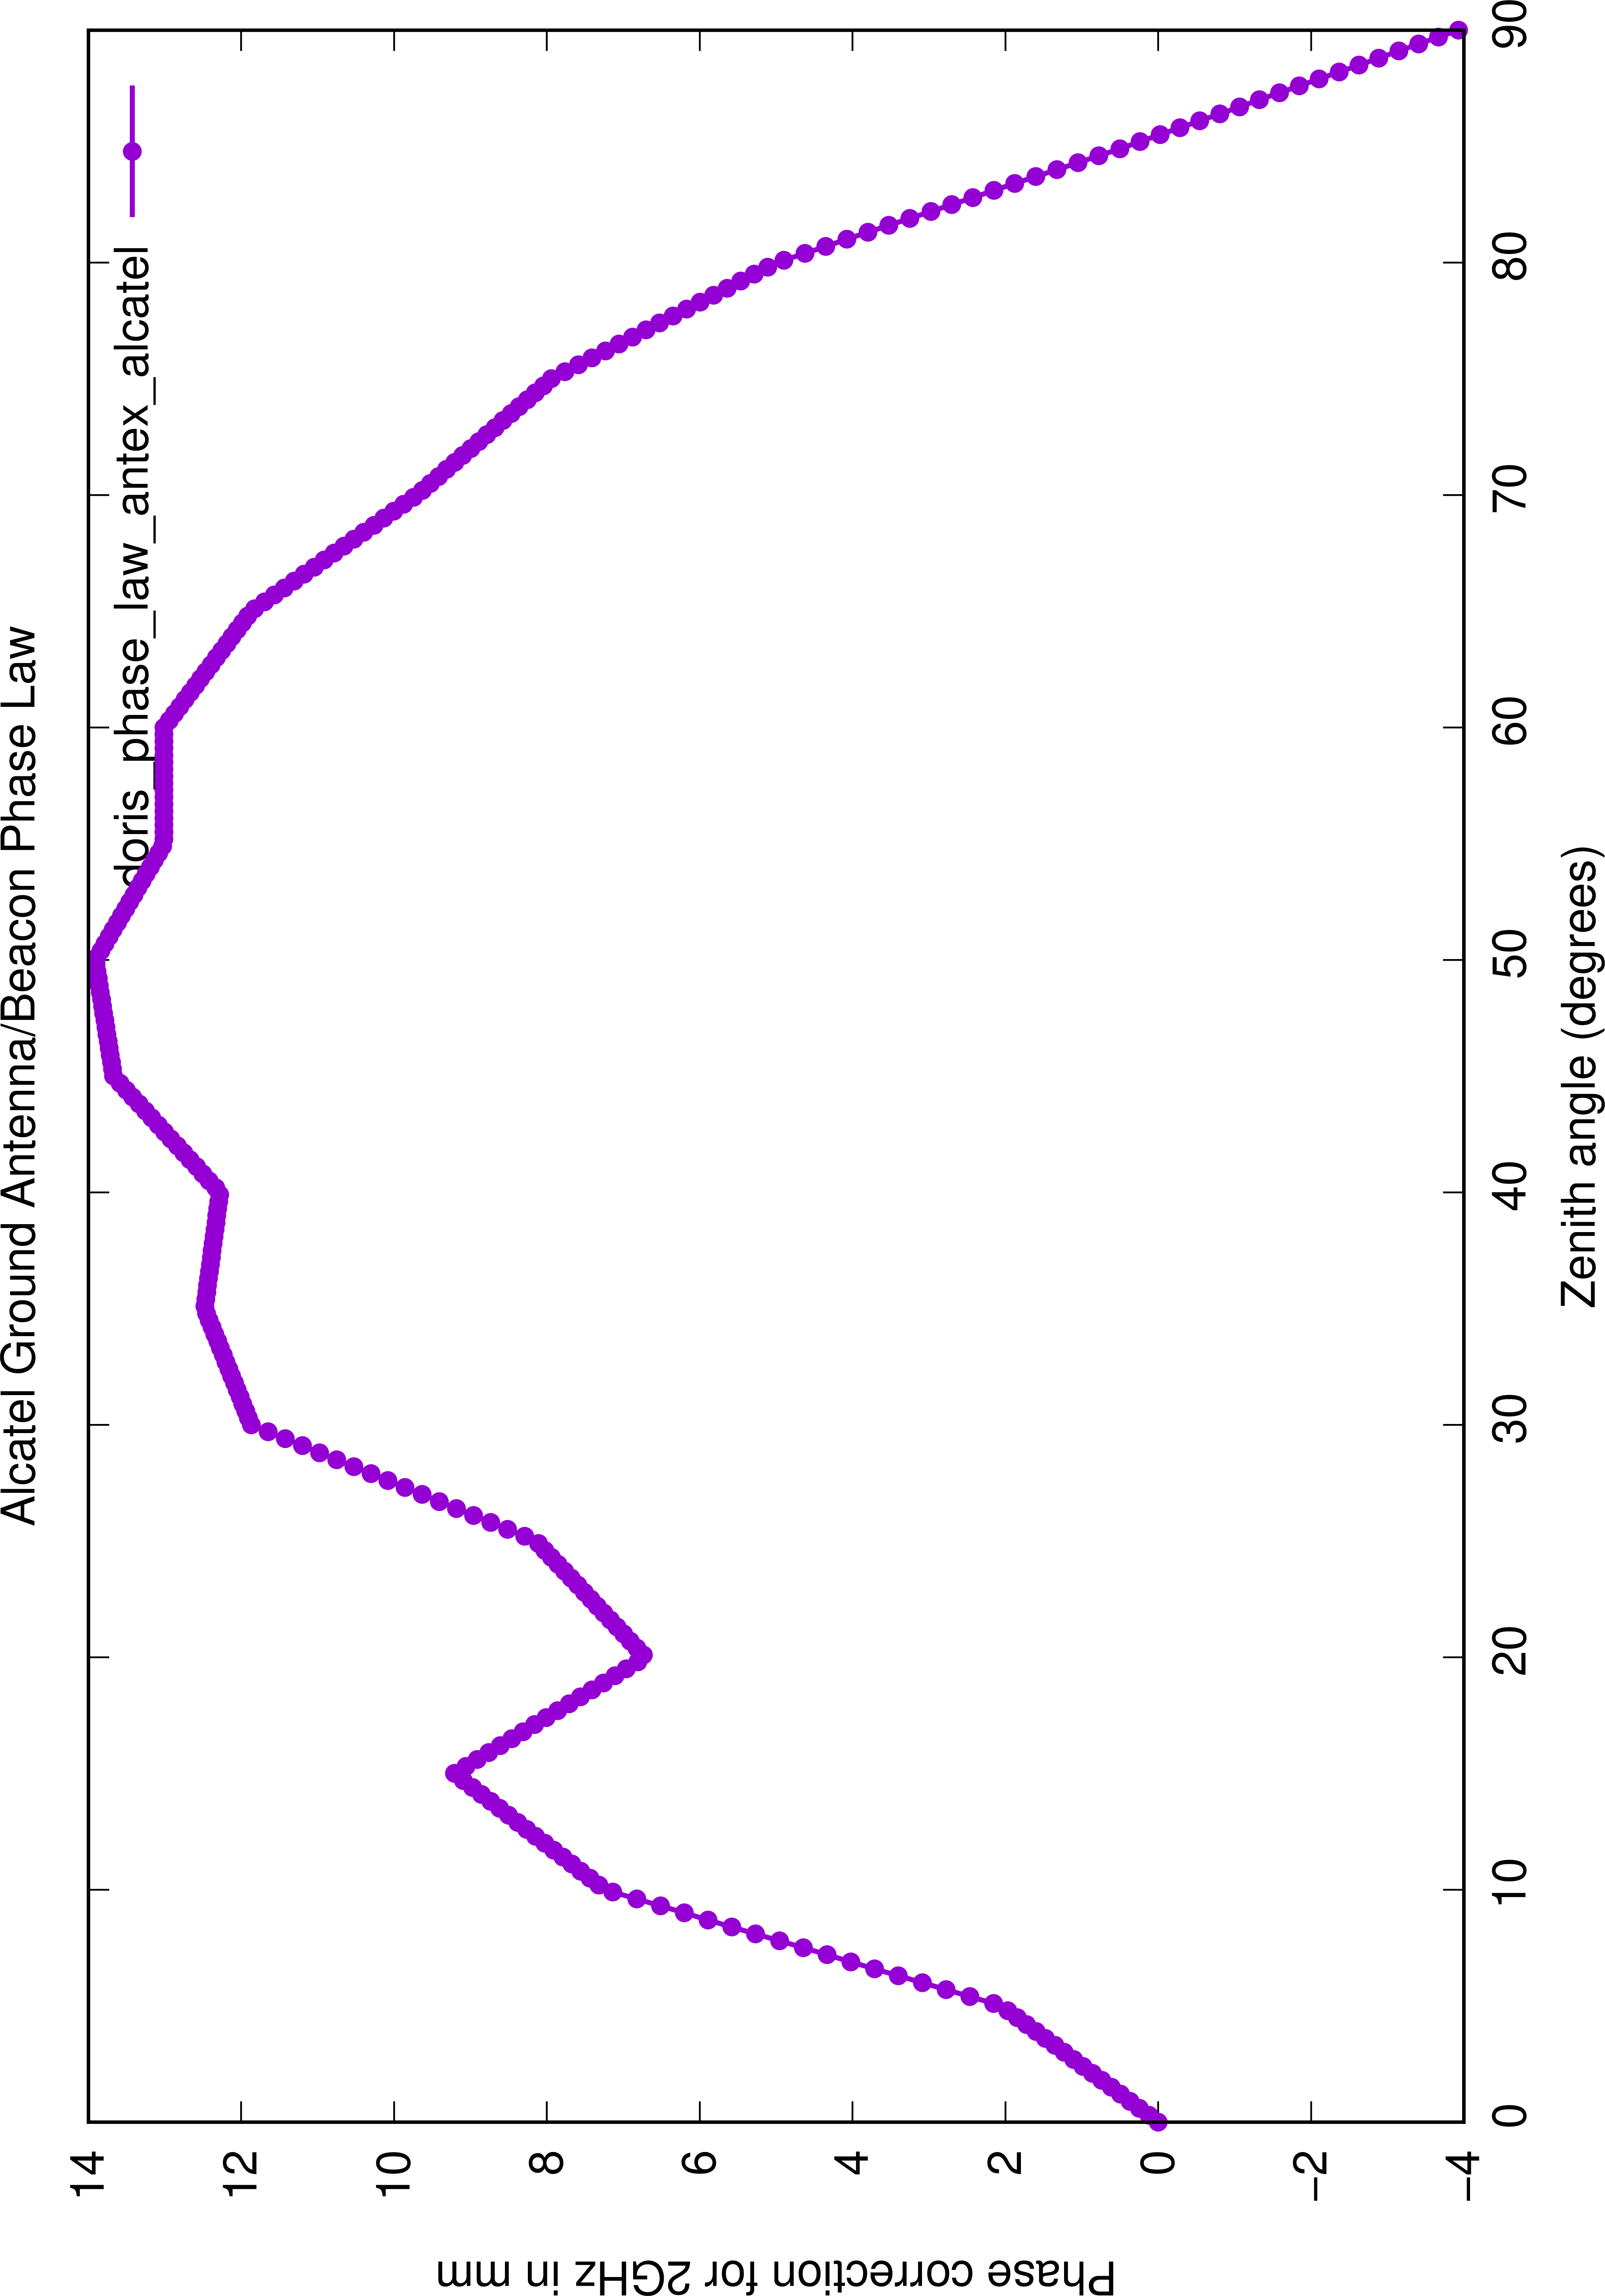
\includegraphics[width=.65\linewidth, angle=-90]{alcatel-phlaw}  
%  \caption{\scriptsize ALCATEL DORIS Ground Antenna Phase Law}
%  \label{fig:pcv-alcatel}
%\end{subfigure}
%\begin{subfigure}{0.45\textwidth}
%  \centering
%  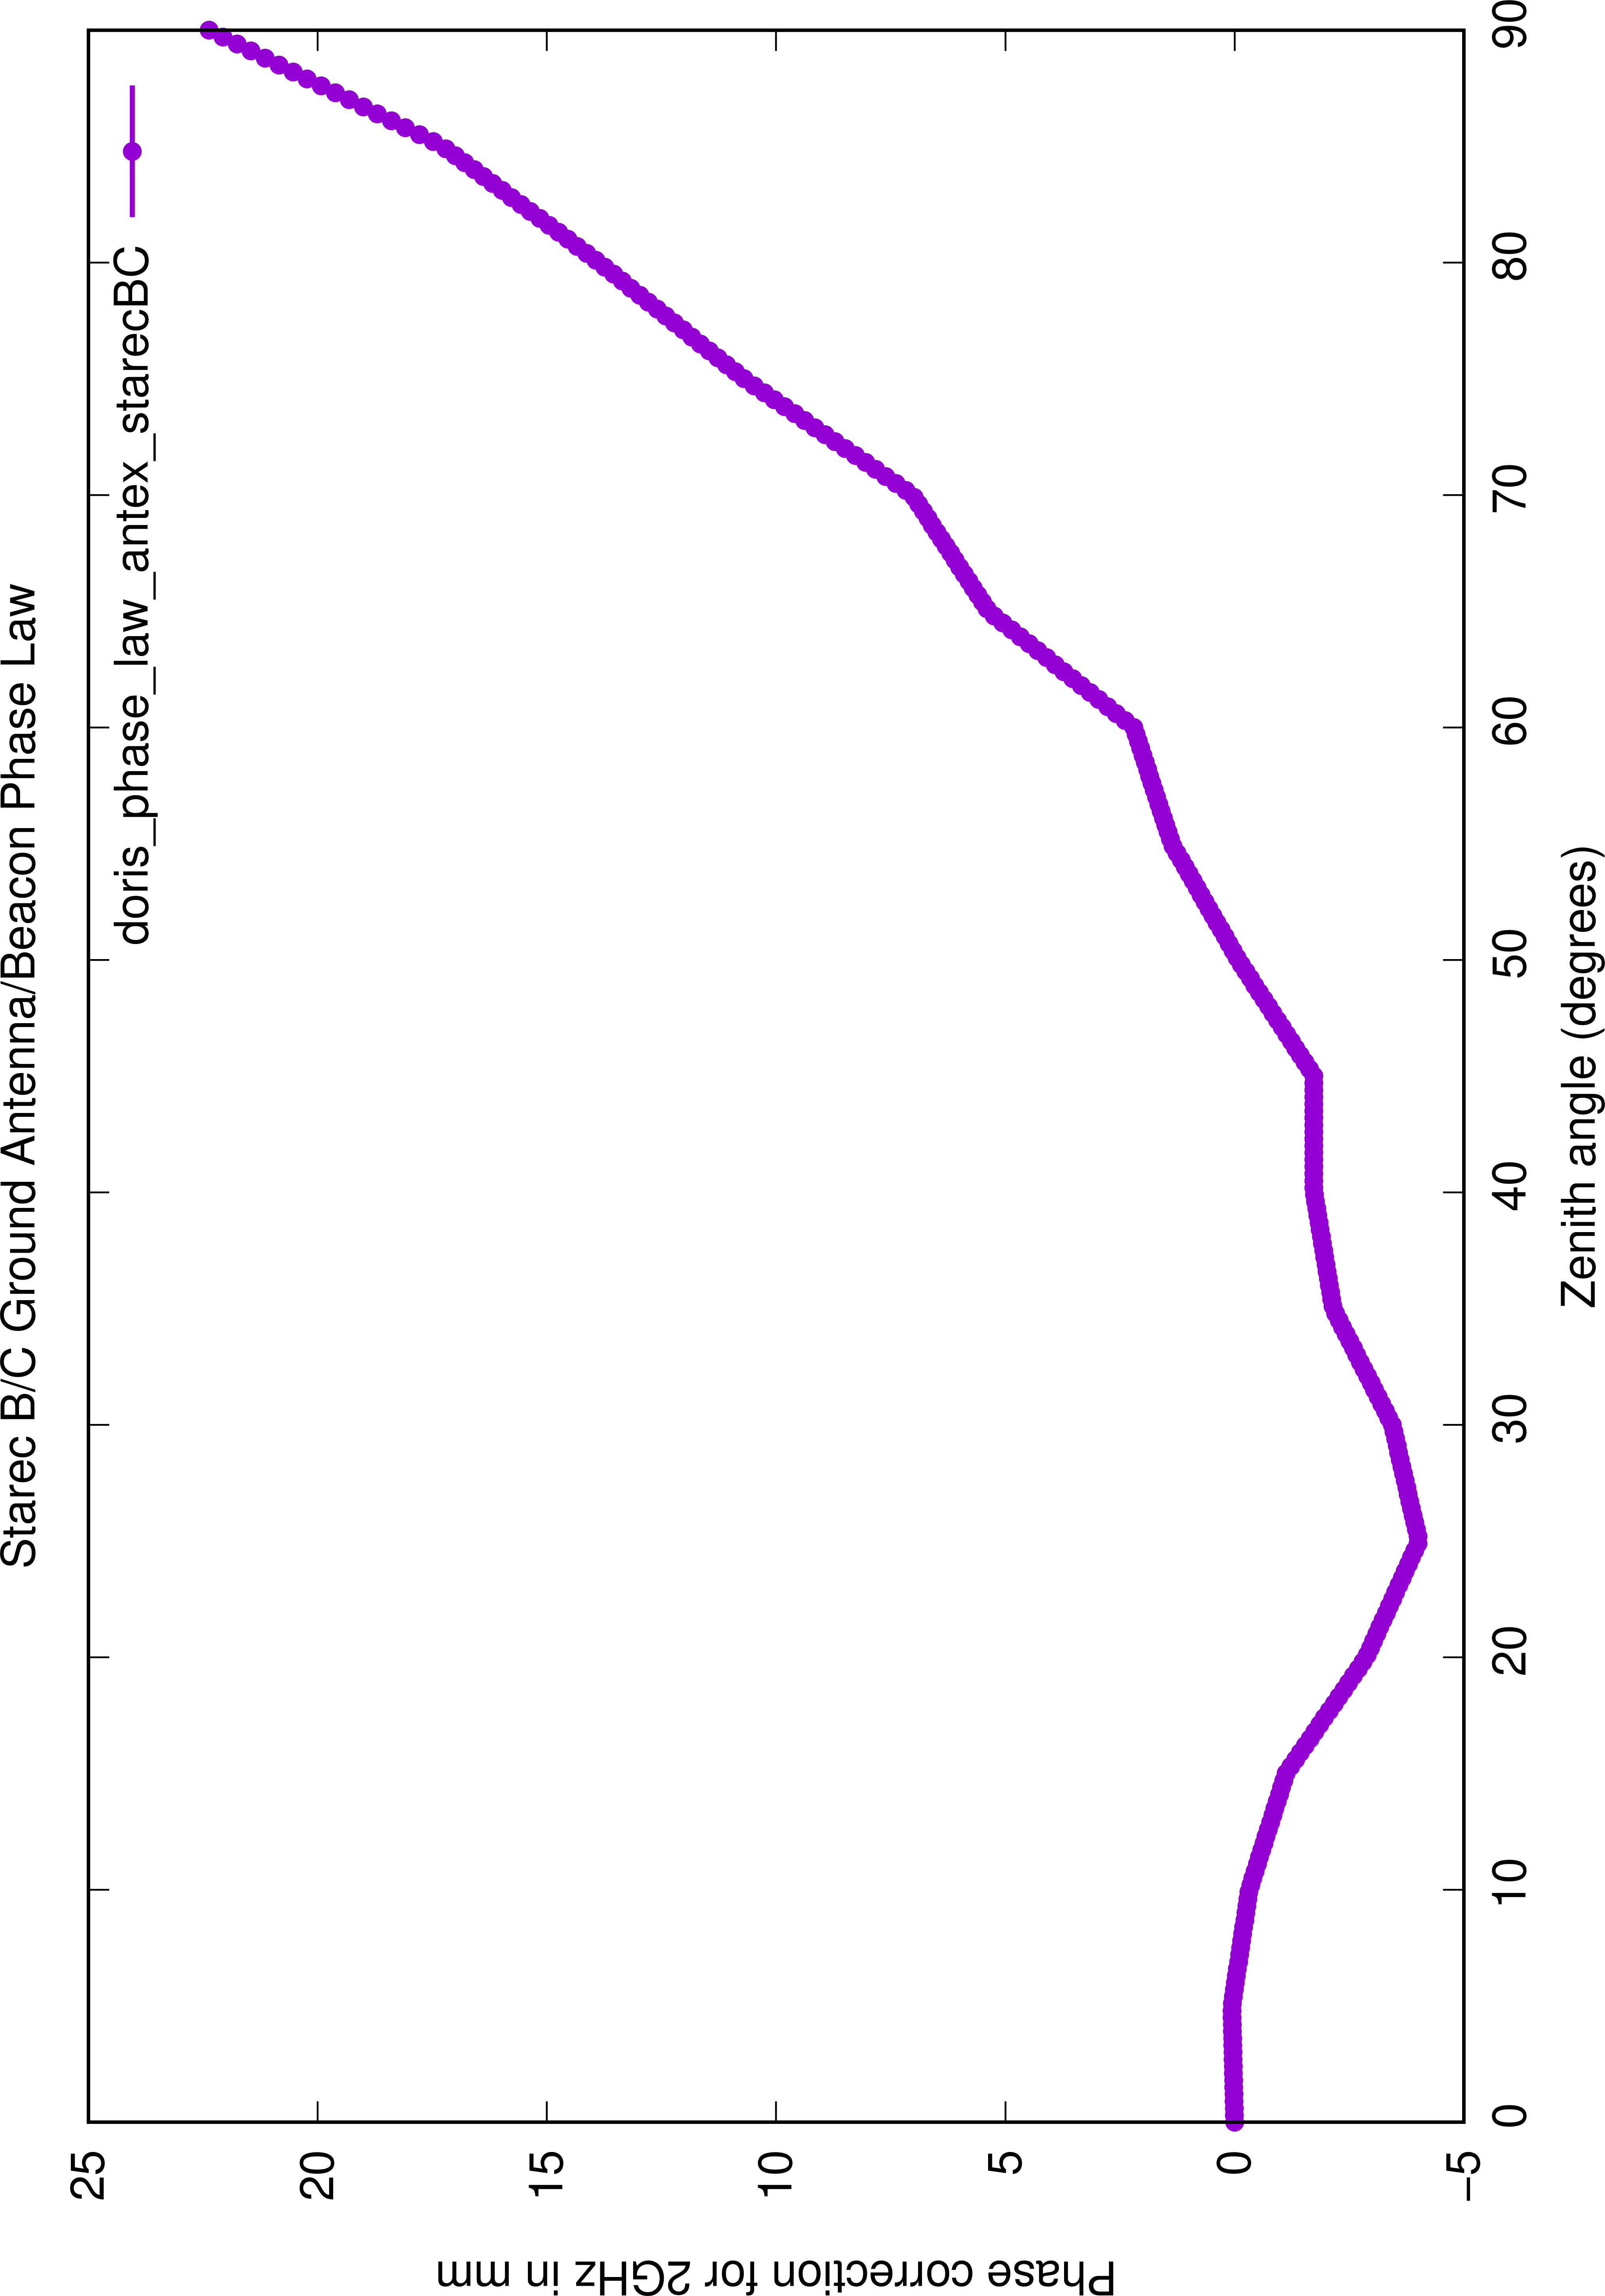
\includegraphics[width=.65\linewidth, angle=-90]{starecbc-phlaw}  
%  \caption{\scriptsize STAREC B/C DORIS Ground Antenna Phase Law}
%  \label{fig:pcv-starec}
%\end{subfigure}
%\caption{DORIS Ground Antenna Phase Law}
%\label{fig:ground-antenna-phase-law}
%\end{figure}

  \section{\gls{doris} Observation Equation}\label{sec:doris-observation-equation}

\subsection{Theoretical Model of Doppler Observations}\label{ssec:doris-obs-theory}
A detailed derivation of the Doppler observation equation, as implemented by means of the 
\gls{doris} system, can be found in \cite{Lemoine2016}, including a thorough theoretical 
discussion. A brief overview is given here, with focus on the measurement model 
implementation.

To gain a clear view on the model of the measurements, a rigorous distinction of 
events must be made; four different events can be identified:
\begin{description}
    \item[beginning of emission] of the 1\textsubscript{st} cycle by the emitter, 
    \(\tau_{e_1}\) in the proper time scale of the emitter and \(t_1\) in the coordinate 
    time
    
    \item[beginning of reception] of the 1\textsubscript{st} cycle by the receiver, 
    \(\tau_{r_1'}\) in the proper time scale of the receiver and 
    \(t_{1'}\) in the coordinate time

    \item[end of emission] of the N\textsubscript{th} cycle by the emitter, 
    \(\tau_{e_2}\) in the proper time scale of the emitter and \(t_2\) in the coordinate 
    time
    
    \item[end of reception] of the N\textsubscript{th} cycle by the receiver, 
    \(\tau_{r_2'}\) in the proper time scale of the receiver and 
    \(t_{2'}\) in the coordinate time
\end{description}

During the proper time interval $\Delta\tau_{r} = \tau_{r2'} - \tau_{r1'}$, 
the receiver has received the $N_e$ cycles sent by the emitter, with $N_e = f_e \Delta\tau_e$, 
$f_e$ being the proper frequency of the emitter. The receiver is also equipped with
an oscillator and during the proper time interval $\Delta\tau_{r}$ has generated 
a number $N_r = f_r \Delta\tau_r$ of cycles, $f_r$ being the proper frequency of the 
receiver.

The Doppler measurement is the count, by the receiver electronics, of the number 
of cycles of difference between \(N_e\) and \(N_r\):
\begin{equation}
    \begin{split}
    N_{DOP} & = N_e - N_r\\
            & = f_e \Delta\tau_e - f_r \Delta\tau_r
    \end{split}
\end{equation}

\emph{In the RINEX files, this Doppler count is the difference between two phase measurements 
done at different time tags in the proper time-scale of the receiver.}

After a series of assumptions and simplifications, theoretical formula for the 
Doppler count can be written as (\cite{Lemoine2016}):
\begin{equation}
    \begin{split}
        \frac{c}{f_e \Delta\tau_r} N_{DOP} & \approx c \frac{f_e - f_r}{f_e} \\
        & - (1 - \frac{U_e}{c^2} - \frac{{V_e}^2}{2 c^2}) \frac{\rho_2 - \rho_1}{\Delta\tau_r}\\
        & + \frac{1}{c} (U_r - U_e + \frac{{V_r}^2 - {V_e}^2}{2}) \\
        & + \frac{2 \mu}{c^2 \Delta\tau_r} [\ln{(\frac{R_1 + R_{1'} + \rho_1}{R_1 + R_{1'} - \rho_1})} - \ln{(\frac{R_2 + R_{2'} + \rho_2}{R_2 + R_{2'} - \rho_2})}]
    \end{split}
\end{equation}
where
\begin{description}
  \item $c$ is the velocity of light in vacuum,
  \item $f_e$ and $f_r$ are the emitter's and receiver's proper frequencies,
  \item $U_e$ and $U_r$ are the gravitational potential at the emitter and receiver,
  \item $V_e$ and $V_r$ is the velocity of the clock at the emitter and receiver 
    (in the coordinate reference frame),
  \item $\rho _i$ is the curvlinear trajectory (of the photon(s)) at the event $i$,
  \item $R_i$ is the geometric distance between the beacon and the satellite at event $i$
\end{description}

The above equation can be conveniently split into two parts, one containing the ``measured'' 
quantities and one with the ``theoretical'' terms, as 
\begin{subequations}\label{eq:lem12}
  \begin{align}
    v_{measured} & = \frac{c}{f_e} (f_e - f_r -
     \frac{N_{DOP}}{\Delta\tau_r}) + \Delta u_{REL} \label{eq:lem12a} \\
    v_{theo}     &= \frac{\rho_2 - \rho_1}{\Delta\tau_r} (1- \frac{U_e}{c^2} - 
      \frac{{V_e}^2}{2 c^2}) \label{eq:lem12b}
  \end{align}
\end{subequations}
with
\begin{equation}
    \begin{split}
        \Delta v_{REL} &= \frac{1}{c} (U_r - U_e + \frac{{V_r}^2 - {V_e}^2}{2}) \\
        & + \frac{2 \mu}{c^2 \Delta\tau_r} [\ln{(\frac{R_1 + R_{1'} + \rho_1}{R_1 + R_{1'} - \rho_1})} - \ln{(\frac{R_2 + R_{2'} + \rho_2}{R_2 + R_{2'} - \rho_2})}]
    \end{split}
\end{equation}

It is well known that signals transmitted through the Earth's atmosphere are 
affected by it (delayed); let $\Delta v_{IONO}$ and $\Delta v_{TROPO}$, be the 
propagation corrections of the radio electric signal through the ionosphere and 
troposphere respectively. 

Additionally, in the actual case (measurements), the nominal frequencies $f_e$ and $f_r$ 
are not the ``true'' ones; hence, a relative correction needs to be applied e.g. for the 
emitter $f_{e_T} = f_{e_N} (1 + \frac{\Delta f_e}{f_{e_N}})$, where the subscript $T$ 
denotes the ``True'' frequency and $N$ the nominal one. Thus in \autoref{eq:lem12} the 
terms $f_e$ and $f_r$ need to be substituted by $f_{e_T}$ and $f_{r_T}$ respectively.

$\Delta v_{IONO}$ and $\Delta v_{REL}$, which do not involve adjusted parameters, can be placed 
on the ``measured'' part of \autoref{eq:lem12} and $\Delta v_{TROPO}$ and $\frac{\Delta f_e}{f_{e_N}}$ 
on the ``theoretical'' part. Furthermore, since $\Delta f_e / f_{e_N} \ll 1$ all  
terms including $\Delta f_e / f^2_{e_N}$ and $\left(\Delta f_e / f_{e_N}\right)^2$ 
can be safely neglected and \autoref{eq:lem12} can be rewritten as:
\begin{subequations}\label{eq:lem13}
    \begin{align}
        v_{measured} & = \frac{c}{f_{e_N}} (f_{e_N} - f_{r_T} -
          \frac{N_{DOP}}{\Delta\tau_r}) + \Delta u_{REL} + 
          \Delta u_{IONO} \label{eq:lem13a} \\
        v_{theo} &= \frac{\rho_2 - \rho_1}{\Delta\tau_r} 
          (1- \frac{U_e}{c^2} - \frac{{V_e}^2}{2 c^2}) + 
          \Delta u_{TROPO} - \frac{c(\frac{N_{DOP}}{\Delta\tau_r} + 
          f_{r_T})}{f_{e_N}} \frac{\Delta f_e}{f_{e_N}} \label{eq:lem13b}
    \end{align}
\end{subequations}
where 
\begin{description}
    \item[$v_{measured}$] is the measured relative velocity between the emitter and 
    the receiver between the events 1' and 2', based on the Doppler count $N_{DOP}$, 
    corrected for the ionospheric and relativistic effects.

    \item[$v_{theo}$] is the theoretical (computed) emitter/receiver relative velocity 
    between the events 1' and 2', corrected for the tropospheric effect and for a solved-for 
    frequency bias $\frac{\Delta f_e}{f_{e_N}}$ of the emitter. 
    $f_{r_T} = f_{r_N} (1 + \frac{\Delta f_r}{f_{r_N}})$ 
    is an estimate of the proper frequency of the receiver.

    \item[$\Delta v_{REL} = \Delta v_{{REL}_c} + \Delta v_{{REL}_r}$] is the relativistic 
    correction, composed of two parts: the clock correction $\Delta v_{{REL}_c}$ and the 
    travel correction $\Delta v_{{REL}_r}$
    \begin{subequations}\label{eq:lem14}
        \begin{align}
            \Delta v_{{REL}_c} & = \frac{1}{c} 
              (U_r - U_e + \frac{{V_r}^2 - {V_e}^2}{2}) \label{eq:lem14a}\\
            \Delta v_{{REL}_r} & = \frac{2 \mu}{c^2 \Delta\tau_r} \left[ 
              \ln{(\frac{R_1 + R_{1'} + \rho_1}{R_1 + R_{1'} - \rho_1})} - 
              \ln{(\frac{R_2 + R_{2'} + \rho_2}{R_2 + R_{2'} - \rho_2})} \right] \label{eq:lem14b}
        \end{align}
    \end{subequations}
\end{description}

Note that \autoref{eq:lem13a} and \autoref{eq:lem13b} can be further simplified 
to \autoref{eq:lem17a} and \autoref{eq:lem17b} respectively, by 
omitting small terms (\autoref{sssec:small-terms}).

\subsection{Computational Aspects}\label{ssec:doris-computational-aspects}

\subsubsection{Small Terms}\label{sssec:small-terms}
In \autoref{eq:lem13a} and \autoref{eq:lem13a}, the smallest terms are $-U_e / c^2 - {V_e}^2 / 2 c^2$ and 
$\Delta v_{{REL}_T}$; in the case of \gls{doris} they amount to \num{11.} and 
\num{6.} \SI{10e-6}{\meter\per\second} respectively (\cite{Lemoine2016}). 
Furthermore, since the emitters are located on the ground, the term 
$-U_e / c^2 - {V_e}^2 / 2 c^2$ is constant per station. This small 
relativistic offset is absorbed by the adjustment of $\Delta f_e / f_{e_N}$. 
So it is possibly to further simplify \autoref{eq:lem13a} and \autoref{eq:lem13b} 
to:
\begin{subequations}\label{eq:lem17}
    \begin{align}
        v_{measured} & = \frac{c}{f_{e_N}} (f_{e_N} - f_{r_T} -
          \frac{N_{DOP}}{\Delta\tau_r}) + 
          \Delta u_{{REL}_C} + \Delta u_{IONO} \label{eq:lem17a}\\
        v_{theo} &= \frac{\rho_2 - \rho_1}{\Delta\tau_r} + \Delta u_{TROPO} - 
          \frac{c(\frac{N_{DOP}}{\Delta\tau_r} + f_{r_T})}{f_{e_N}} 
          \frac{\Delta f_e}{f_{e_N}} \label{eq:lem17b}
    \end{align}
\end{subequations}

\subsubsection{Correction of Aberration}\label{sssec:doris-aberration}
In \autoref{eq:lem13b} (or \autoref{eq:lem17b}), $\rho _i$ is the geometrical distance 
between the emitter at time $t_i$ and the receiver at time $t_{i'}$ (with $i=1,2$). 
The measurements are made by the receiver electronics, hence the instance $t_i$ is 
actually unknown. In order to compute accurately $t_i$ and thus the position of 
the emitter at this instant in time, a \emph{correction of aberration} (\cite{Lemoine2016}) 
has to be performed. This correction can be evaluated in an iterative manner: an 
approximate value of the emitter-receiver distance $\rho ^{*} _i$ is first computed, 
by evaluating the position of the beacon at time $t_{i'}$. Subsequently, $t_i$ can be 
found via $t_i = t_{i'} - \rho ^{*} _i / c$. In practice, one iteration is enough.

\subsubsection{Geopotential}\label{sssec:doris-geopotential}
For a station on the geoid, the potential at the level of the station is the sum 
of the gravitational potential and the centrifugal potential due to the Earth's 
rotation: $U_{GEO} = U_e + \frac{{V_e}^2}{2}$, which is a constant. For a station 
not located on the geoid, the quantity $U_e + \frac{{V_e}^2}{2}$ will only depend 
on the height of the beacon above the geoid.

For the computation of the gravitational potential for \gls{leo} satellites, 
the potential $U_r$ cannot be restricted to the central term only ($GM_{\Earth} / r$) and
the Earth's oblateness ($J_2$) effect should also be considered (\cite{Larson2007}). 
Hence, the equation used for computing the potential for a given satellite, reads 
(\cite{Lemoine2016})
\begin{equation}\label{eq:lem18}
  U_r = 
    -\frac{GM_{\Earth}}{r} \left( 
      1 - 
      \left( \frac{R_{\Earth}}{r} \right) ^2 
      J_2 \frac{3 sin^2(\phi) - 1}{2} 
    \right)
\end{equation}
or in Cartesian coordinates (\cite{Larson2007})
\begin{equation}
  U_r = -\frac{GM_{\Earth}}{r} \left( 1- \left(\frac{R_{\Earth}}{r}\right)^2 
    J_2 \frac{3 z^2 - r^2}{2r^2} \right)
\end{equation}
with $R_{\Earth}$ the equatorial radius of the earth, $r$ radial 
distance of the satellite (to the Earth's center), $\phi$ latitude of the 
satellite and $J_2 = 1.0826359 \dot 10^{-3}$ in the zero-tide system (\cite{iers2010}).

\iffalse
\subsubsection{True Proper Frequency of the Receiver}\label{sssec:true-proprtfrequency-of-the-receiver}
For the term $f_{r_T}$ that appears in \autoref{eq:lem13a} and \autoref{eq:lem13b}, we need an estimate of 
$\Delta f_{r} / f_{r_N}$. This estimate can be obtained in one of the following ways 
\cite{Lemoine2016}:
\begin{enumerate}
    \item Via the field ``F'' recorded for every single measurement in the \gls{doris} 
      RINEX file (see \autoref{ssec:relative-frequency-offset}); not that this estimation 
      is not very smooth, as noticed by \cite{Gao2015} and it is advisable, before 
      using it in \autoref{eq:lem13}, to perform a linear (or polynomial) regression of 
      these estimates over one or a few days.
    \item It can be obtained from a polynomial regression over the frequency 
      offsets estimated during the passes over the master beacons
    \item It can be estimated as a by-product during a re-computation of the 
      ``timetagging'' polynomial (see \cite{Mercier2010})
\end{enumerate}
\fi

\subsubsection{Nominal Receiver and Emitter Frequencies}\label{ssec:nominal-frequencies}
In the observation equation model \autoref{eq:lem13a} and \autoref{eq:lem13b}, a distinction is made between 
\emph{nominal} and \emph{true} receiver/emitter frequencies, to account for the 
fact that in ``real world'' these two are not actually equal.

\paragraph{Emitter (Beacon) Nominal Frequencies, $f_{e_N}$}\label{par:beacon-nominal-frequencies}
RINEX file headers, contain values of the \emph{station frequency shift 
factor} $k$ for each of the beacons involved (\cite{DORISRNX3}, Sec. 6.16). 
These are used to compute the ``nominal'' frequencies of the beacon/emitter 
(usually, this shift factor is just $0$, but it can be an integer 
$k \neq 0$). The frequencies are computed as (\cite{DORISRNX3}, Sec. 6.16):
\begin{equation}
  \begin{aligned}
    L_{2GHz}   &= 543 \cdot F_0 \left( \frac{3}{4} + \frac{87\cdot k}{5 \cdot 2^{26}} \right) \\
    L_{400MHz} &= 107 \cdot F_0 \left( \frac{3}{4} + \frac{87\cdot k}{5 \cdot 2^{26}} \right) 
    \label{eq:nominal-freq}
  \end{aligned}
\end{equation}
where $F_0 = 5e6 \text{ Hz}$ the \gls{uso} frequency. These value, are the ones 
labelled as $f_{e_N}$ in \autoref{eq:lem13a} and \autoref{eq:lem13b}.

The \emph{true proper frequency} of the emitter $f_{e_T}$, can be computed (if needed) 
from:
\begin{equation}
  f_{e_T} = f_{e_N} \cdot \left( 1 + \frac{\Delta f_e}{f_{e_N}} \right)
\end{equation}
but the quantity $\Delta f_e / f_{e_N}$ is not known a-priori and has to be 
estimated during the processing.

The quantity $\Delta f_e / f_{e_N}$  can be estimated either as a constant term (bias), 
or using a linear model (bias ad drift). In the latter case (followed in this Thesis), 
the model can be written as:
\begin{equation}
  \frac{\Delta f_e}{f_{e_N}}\at{\tau=\tau _i} = \alpha + \beta \cdot \delta \tau
\end{equation}
For the estimation, the partials of the observation equation \autoref{eq:lem13b} are needed, 
with respect to $\alpha$ and $\beta$ parameters, which are:
\begin{equation}
  \begin{aligned}
  \frac{\partial v_{theo}}{\partial \alpha} &= 
    \frac{c(\frac{N_{DOP}}{\Delta\tau_r} + f_{r_T})}{f_{e_N}} \\
  \frac{\partial v_{theo}}{\partial \beta} &= 
    \frac{c(\frac{N_{DOP}}{\Delta\tau_r} + f_{r_T})}{f_{e_N}} \cdot \delta \tau
  \end{aligned}
\end{equation}

\paragraph{Receiver True Proper Frequency $f_{r_T}$}\label{par:receiver-true-proper-frequency}
In \autoref{eq:lem13a} and \autoref{eq:lem13b}, $f_{r_T}$ is the \emph{true proper frequency of 
the receiver}, computed as
\begin{equation}\label{eq:frt-gen}
  f_{r_T} = f_{r_N} \cdot \left( 1 + \frac{\Delta f_r}{f_{r_N}} \right)
\end{equation}
where $f_{r_N}$ is the ``nominal'' frequency value. The value of the quantity 
$\Delta f_r / f_{r_N}$, called the \emph{relative frequency offset} of the receiver,
can be extracted from the RINEX file, estimated or computed, in one of the following 
ways (\cite{Lemoine2016})
\begin{enumerate}
    \item Via the field ``F'' recorded for every single measurement in the \gls{doris} 
      RINEX file (see \autoref{sec:doris-rinex}); not that this estimation 
      is not very smooth, as noticed by \cite{Gao2015} and it is advisable, before 
      using it in \autoref{eq:lem13}, to perform a linear (or polynomial) regression of 
      these estimates over one or a few days.
    \item Obtained from a polynomial regression over the frequency 
      offsets estimated during the passes over the master beacons
    \item Estimated as a by-product during a re-computation of the 
      ``timetagging'' polynomial (see \cite{Mercier2010})
\end{enumerate}

Relative frequency offset values, $\frac{\Delta f_r}{f_{r_N}}$, are reported in the RINEX files for each epoch 
(under the observable tagged \texttt{F}). Note that these values are scaled to 
$10^{-11}$ (\cite{DORISRNX3}, Sec. 6.11), so that for a given epoch $t_i$, the 
true frequency is
\begin{equation}\label{eq:frt-rinex}
  f_{r_T}\at{t=t_i} = f_{r_N} \cdot \left( 1 + F_{t_i} \cdot 10^{-11} \right)
\end{equation}
where $F_{t_i}$ is the relative frequency offset value recovered from the RINEX 
file.

\subsection{Ionospheric Correction}\label{ssec:iono-correction}
The basic observation equation \autoref{eq:lem13a} and \autoref{eq:lem13b}, is formed for the \SI{2}{\GHz} 
carrier. For each measurement, the ionospheric path delay has to be corrected for, 
by computing a correction (in cycles) as (\cite{Lemoine2016}, Sec. 2.5.7):
\begin{equation}
  \delta_{ION} [\SI{2}{\GHz}\text{ cycles}] = 
    \frac{L_{\SI{2}{\GHz}} - \sqrt{\gamma} \cdot L_{\SI{400}{\MHz}}}{\gamma - 1}
  \label{eq:iono-delay-cycles}
\end{equation}
which is added to the \SI{2}{\GHz} measurement at time $t=t_i$ (obtained by the 
RINEX file). Thus, the corrected observation is:
\begin{equation}\label{eq:l2if}
  L_{\SI{2}{\GHz},IF} [\SI{2}{\GHz}\text{ cycles}] = 
    L_{\SI{2}{\GHz}} + \delta_{ION}
\end{equation}

Note that after applying \autoref{eq:l2if}, the measurement is referred to the ``Iono-Free'' 
geometrical endpoints of the signal path (and not the \SI{2}{\GHz} endpoints). 
This means that the respective {phase center corrections (i.e. \gls{pco} and \gls{pcv})
both at the satellite and at the beacon have to be applied.

  \chapter{Technicalities}
\label{ch:technicalities}

\section{Software}
\label{se:software}

\begin{figure}
\centering
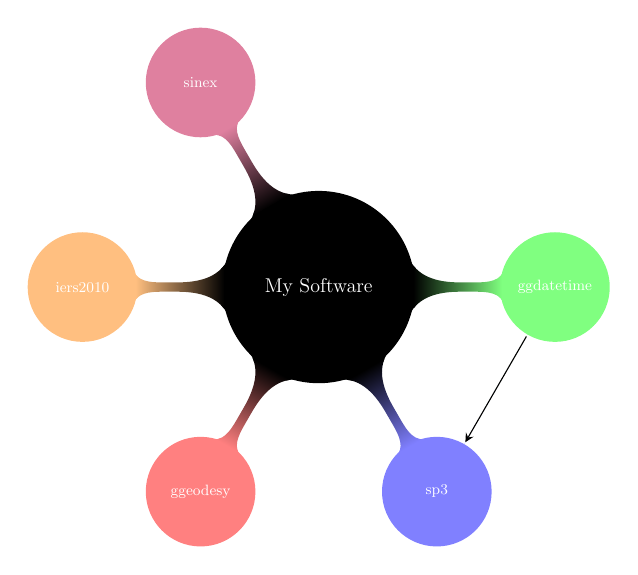
\begin{tikzpicture}[thick,scale=0.6, every node/.style={transform shape}]
  \path[mindmap,concept color=black,text=white]
    node[concept] {My Software}
    [clockwise from=0]
    child[concept color=green!50] {
      node[concept] (ggdatetime) {ggdatetime}
      %[clockwise from=90]
      %child { node[concept] {algorithms} }
    }
    child[concept color=blue!50] {
      node[concept] (sp3) {sp3}
      %[clockwise from=-30]
      %child { node[concept] {databases} }
    }
    child[concept color=red!50]    { node[concept] {ggeodesy} }
    child[concept color=orange!50] { node[concept] {iers2010} }
    child[concept color=purple!50] { node[concept] {sinex} };
    \begin{pgfonlayer}{background}
      \draw [left color=blue!50, 
        right color=green!50, 
        %draw=white, 
        decorate, 
        %decoration=circle connection bar,
        shorten <= 0.05cm, shorten >= 0.05cm,
        -stealth] (ggdatetime) to (sp3);
    \end{pgfonlayer}
\end{tikzpicture}

\caption{Software Structure Tree}
\label{fig:software-structure-tree}
\end{figure}

\section{Dependencies}
\begin{description}
    \item [libcurl] a free, and open-source multiprotocol file transfer library.
    \href{https://curl.se/libcurl/}{libcurl} is highly portable, it builds and works 
    identically on numerous platforms and provides a \href{https://curl.se/libcurl/c/}{C API}, 
    accessing remote files via the C/C++ programming languages. Installation is 
    trivial in most operating systems\footnote{E.g. for Fedora LInux: \lstinline[language=bash]|$ dnf install libcurl libcurl-devel|}.
    
    \item [Eigen] (\cite{eigenweb}) a free, and open-source C++ template library 
    for linear algebra. 
    \href{https://eigen.tuxfamily.org/index.php?title=Main_Page}{Eigen} is a 
    versatile, fast and reliable library, with no dependencies other than the 
    C++ standard library. Since it is a header-only library, ``installation'' 
    and inclusion is very easy for any platform.

    \item [cgem] a free, and open-source C++ library. 
    \href{https://www.kthohr.com/gcem.html}{cgem} offers compile-time 
    computation of a number of widely used mathematical function, see
    \ref{sec:constexpr-math}

\end{description}

\section{Constexpr Math}
\label{sec:constexpr-math}
Currently (\today), the standard C++ library \texttt{math.h} does not offar 
trigonometric mathematical functions qualified as \texttt{constexpr} (see 
\href{https://en.cppreference.com/w/cpp/header/cmath}{Standard library header \texttt{<cmath>}}).
\texttt{constexpr} functions can spped-up computations by performing them at 
compile-time (see 
\href{https://en.cppreference.com/w/cpp/language/constexpr}{\texttt{constexpr} keyword}). 
The \href{https://gcc.gnu.org/onlinedocs/libstdc++/}{GNU C++ Library} 
implementation \texttt{libstdc++} does offer such functions as an extension. It 
was however decided to not use these extensions, because:
\begin{itemize}
    \item they do not conform to the standard,
    \item we want to be able to build with any compiler and standard library implementation
\end{itemize}

Hence, we are using the \href{https://www.kthohr.com/gcem.html}{Generalized Constant Expression Math} 
(\texttt{gsem}) library, when such functionality is needed.

It is expected that in the near future, most of the standard mathematical 
functions will be marked/implemented as \texttt{constexpr} (\cite{rostencpp}). 
When such functionality is offered, the dependency on \texttt{gcem} should be 
dropped in favor of using the standard functions.

Source files affected:
\begin{itemize}
    \item \path{occultation.cpp}
    \item \path{sunpos.cpp}
\end{itemize}

  \chapter{State Transition Matrix and Variational Equations}
\label{ch:state-transition-matrix-and-variational-equations}

The \emph{State Transition Matrix} $\bm{\Phi} (t, t_0 )$, at some specified epoch $t_0$ 
describes the results of a change of initial values (in the state vector 
$\bm{y}(t_0) = \begin{bmatrix} \bm{r}(t_0) \bm{v}(t_0) \end{bmatrix}$)
in a later epoch $t$. The form of the State Transition Matrix, is:
\begin{equation}
  \begin{pmatrix}
    \frac{\partial \bm{y}(t)}{\partial \bm{y}(t_0)}
  \end{pmatrix}_{(6 \times 6)}
  = \bm{\Phi} (t, t_0)
\end{equation}

Besides initial state, the orbit also depends on a number of parameters, 
$\bm{p}$, with size $n_p$, that determine the forces acting on the given 
satellite at a given instant $t$. Such parameters can be, e.g. the drag 
coefficient $C_D$. The dependence of the orbit on these parameters is 
described by the so called \emph{Sensitivity Matrix} $\bm{S}(t)$, where:
\begin{equation}
  \begin{pmatrix}
    \frac{\partial \bm{y}(t)}{\partial \bm{p}}
  \end{pmatrix}_{(6 \times n_p)}
  = \bm{S} (t)
\end{equation}

Denoting an observation by $z(t)$, we can also derive the partials of the 
measurements with respect to the state vector, which is given by the partials
$ \begin{pmatrix} \frac{\partial \bm{z}}{\partial \bm{y}(t)} \end{pmatrix}_{(1 \times 6)}$

Computation of the observation model also depends on a number of 
parameters $\bm{q}$, of size $n_q$, such as e.g. relative frequency offsets, 
wet part of zenith tropospheric delay, etc. The dependance of the predicted 
observation values on these parameters, is described by the partials:
$ \begin{pmatrix} \frac{\partial \bm{z}}{\partial \bm{q}} \end{pmatrix}_{(1 \times n_q)}$

Combining the above, we can compute the dependence of an individual measurement 
$z$ on the initial state vector $\bm{y}(t_0)$, force model parameters $\bm{p}$ 
and observation model parameters $\bm{q}$ (\cite{Montenbruck2000}):
\begin{equation}
  \begin{pmatrix}
    \frac{\partial \bm{z}}{\partial \bm{y}(t_0)}, 
    \frac{\partial \bm{z}}{\partial \bm{p}}, 
    \frac{\partial \bm{z}}{\partial \bm{q}}
  \end{pmatrix}_{(1 \times (6+n_p+n_q))} = 
  \begin{pmatrix}
    \left( \frac{\partial \bm{z}}{\partial \bm{y}(t)} \right)
    \left( \Phi (t,t_0) \bm{S}(t) \right), 
    \frac{\partial \bm{z}}{\partial \bm{q}}
  \end{pmatrix}
\end{equation}

In applications where accuracy demands are high, the computation of the state 
transition matrix $\bm{\Phi}(t,t_0)$, must take into account at least the major 
perturbations. As is the case for perturbed motion, this augmentation make an 
analytical solution impossible; one has to solve a set of differential equations, 
the so-called ``\emph{Variational Equation}'' by numerical methods.

The state vector $\bm{y}(t) = \begin{bmatrix} \bm{r}(t) \\ \bm{v}(t) \end{bmatrix}$ 
obeys the first order differential equation:
\begin{equation}
  \frac{d \bm{y}(t)}{dt} = \bm{f}(t,\bm{y}) = 
    \begin{bmatrix} \bm{v}(t) \\ \bm{a}(t,\bm{r},\bm{v}) \end{bmatrix}
\end{equation}
so that:
\begin{equation}
  \frac{\partial}{\partial \bm{y}(t_0)}\frac{d\bm{y}(t)}{dt} = 
    \frac{\partial \bm{f}(t,\bm{y}(t))}{\partial \bm{y}(t_0)} = 
    \frac{\partial \bm{f}(t,\bm{y}(t))}{\partial \bm{y}(t)} 
      \frac{\partial \bm{y}(t)}{\partial \bm{y}(t_0)}
\end{equation}

The state transition matrix
\begin{equation}
  \bm{\Phi}(t,t_0) = \frac{\partial \bm{y}(t)}{\partial \bm{y}(t_0)}
\end{equation}

may therefore be obtained from:
\begin{equation}
  \frac{d}{dt}\bm{\Phi}(t,t_0) = 
    \frac{\partial \bm{f}(t,\bm{y}(t))}{\partial \bm{y}(t)}
      \bm{\Phi}(t,t_0)
\end{equation}

or

\begin{equation}
  \frac{d}{dt}\bm{\Phi}(t,t_0) = 
  \begin{bmatrix}
    \bm{0}_{(3 \times 3)} & \bm{I}_{(3 \times 3)} \\
    \frac{\partial \bm{a}(t,\bm{r},\bm{v})}{\partial \bm{r}(t)} &
      \frac{\partial \bm{a}(t,\bm{r},\bm{v})}{\partial \bm{v}(t)} \\
  \end{bmatrix}_{(6 \times 6)}
  \bm{\Phi}(t,t_0)
\end{equation}

with the initial condition:
\begin{equation}
  \bm{\Phi}(t_0,t_0) = \bm{I}_{(6 \times 6)}
\end{equation}

In an analogous way, we can derive the differential equation of the sensitivity 
matrix (partial derivatives of the state vector \emph{w.r.t} the force model 
parameter vector $\bm{p}$):
\begin{equation}
  \begin{pmatrix} \frac{d}{dt} \frac{\partial \bm{y}(t)}{\partial \bm{p}} 
    \end{pmatrix}_{(6 \times 6)} = 
  \frac{\partial \bm{f}(t,\bm{y}(t), \bm{p})}{\partial \bm{y}(t)} 
      \frac{\partial \bm{y}(t)}{\partial \bm{p}} + 
      \frac{\partial \bm{f}(t,\bm{y}(t), \bm{p})}{\partial \bm{p}}
\end{equation}
or:
\begin{equation}
  \begin{pmatrix} \frac{d}{dt}\bm{S}(t) \end{pmatrix}_{6 \times n_p} = 
    \begin{pmatrix}
      \bm{0}_{(3 \times 3)} & \bm{I}_{(3 \times 3)} \\
      \frac{\partial \bm{a}(t,\bm{r},\bm{v},\bm{p})}{\partial \bm{r}(t)} &
      \frac{\partial \bm{a}(t,\bm{r},\bm{v},\bm{p})}{\partial \bm{v}(t)}
   \end{pmatrix}_{(6 \times 6)}
    \bm{S}(t) + 
   \begin{pmatrix}
      \bm{0}_{(3 \times n_p)} \\
      \frac{\partial \bm{a}(t,\bm{r},\bm{v},\bm{p})}{\partial \bm{p}}
   \end{pmatrix}_{(6 \times n_p)}
\end{equation}

with initial conditions $\bm{S}(t_0) = \bm{0}$, since the state vector at $t_0$ 
does not depend on the force model parameters.

The set of variational equations are formulated by augmenting the differential 
equation system of the state transition matrix, with the one derived from the 
sensitivity matrix; hence, we have:
\begin{equation}
  \frac{d}{dt} \begin{pmatrix} \bm{\Phi} & \bm{S} \end{pmatrix} = 
  \begin{pmatrix}
      \bm{0}_{(3 \times 3)} & \bm{I}_{(3 \times 3)} \\
      \frac{\partial \bm{a}}{\partial \bm{r}} & \frac{\partial \bm{a}}{\partial \bm{v}} 
  \end{pmatrix}_{(6 \times 6)}
  \cdot \begin{pmatrix} \bm{\Phi} & \bm{S} \end{pmatrix} + 
  \begin{pmatrix}
      \bm{0}_{(3 \times 6)} & \bm{0}_{(3 \times n_p)} \\
      \bm{0}_{(3 \times 6)} & \frac{\partial \bm{a}}{\partial \bm{p}} 
  \end{pmatrix}_{(6 \times (6+n_p))}
\end{equation}
More suitable representations of the above differential equation systems can be 
formulated, when choosing to directly integrate the set of second order 
differential equations (see e.g. \cite{Montenbruck2000}).

It is important to note, that the variational equations must be integrated 
simultaneously. 

  \chapter{Orbit Determination}
\label{ch:orbit-determination}

\section{Orbit Determination via DORIS}
\label{sec:pod}

We will use an Extended Kalman Filter to perform the orbit determination. The 
filter's parameter vector will be the satellite state, plus two parameters per 
beacon for the zenith tropospheric wet delay ($L^w_z$) and the relative frequency 
offset ($\Delta f$), that is:
$\bm{X}=
    \begin{pmatrix}
        r_x & r_y & r_z & \dot{r}_x & \dot{r}_y & \dot{r}_z 
        \begin{pmatrix} L^w_z & \frac{\Delta f_e}{f_{eN}} \end{pmatrix}_{beacon_1} & 
        \begin{pmatrix} L^w_z & \frac{\Delta f_e}{f_{eN}} \end{pmatrix}_{beacon_2} &
        \cdots 
    \end{pmatrix}^T$
with size=$6+2 \times \text{ num of beacons} = N$

\subsection{Initialization} \label{ssec:Initialization}
Let's say we have a DORIS RINEX file with the first (block of) observations 
taken at some time $t_i$ (in TAI). We search through a corresponding sp3 file, 
to get the state of the satellite at an epoch as close as possible to $t_i$; 
Let's call this epoch $t_0$ and the satellite state at this epoch (extracted 
from the sp3) as $\bm{y}_0$.

\subsection{Integration} \label{ssec:integration}
Starting from initial conditions $\bm{y}_0 \text{ at } t_0$, and 
$\bm{\Phi} (t_0,t_0) = \bm{I}_{(6 \times 6)}$, we use the integrator 
(see \ref{sec:Integrator}) to get the state and state transition matrix at $t_i$, 
that is we compute 
$\bm{y}(t=t_i) = \begin{pmatrix} \bm{r}^T(t=t_i) & \bm{v}^T(t=t_i) \end{pmatrix}$ 
and $\bm{\Phi} _{t_i}$.

\subsection{Time Update} \label{ssec:time-update}
Perform the \emph{time update} for the Kalman Filter:
\begin{enumerate}
    \item Set the filter time variable to $t=t_i$,
    \item Update the satellite state in the filter parameters vector $\bm{X}$, 
        that is: $\bm{X}_{t_i} = \begin{pmatrix} \bm{r}^T_{t_i} & \bm{v}^T_{t_i} & \bm{X}[6:N] \end{pmatrix}$
    \item Use the $\bm{\Phi}$ matrix to update the var-covariance matrix; the 
        propagation for the non-state elements of $\bm{X}$, is performed using 
        the identity matrix:
        \begin{equation}
            P_{t_i} = \begin{pmatrix} \bm{\Phi} & \bm{0} \\ \bm{0} & \bm{I} \end{pmatrix} 
                P_{t_{i-1}} 
                \begin{pmatrix} \bm{\Phi} & \bm{0} \\ \bm{0} & \bm{I} \end{pmatrix} ^T
        \end{equation}
\end{enumerate}

\subsection{Measurement Update} \label{ssec:measurement-update}
Now start filtering for the current epoch (in the RINEX file) $t_i$. For each 
beacon/observation in the current block:
\begin{enumerate}

    \item If this is the first observation for this beacon, store measurements 
        and exit. If we already have previous measurements for the beacon (so 
        that we can compute the Doppler count), formulate the observation 
        equation, using the two quantities:
        \begin{equation}
            \begin{aligned}
              V_{observed} &= \frac{c}{f_{eN}} 
                \left( f_{eN} - f_{rT} - \frac{N_{DOP}}{\Delta _{\tau_r}} \right)
                + \Delta _{V_{IONO}} + \Delta _{V_{REL_C}} \\
              V_{theoretical} &= \frac{\rho(t_i) - \rho(t_{i-1})}{\Delta _{\tau_r}} + \Delta _{V_{TROPO}} 
                - \frac{c}{f_{eN}} \left( \frac{N_{DOP}}{\Delta _{\tau_r}} + f_{rT} \right) 
                \frac{\Delta f_e}{f_{eN}}
            \end{aligned}
          \end{equation}
        so that $z_i = V_{observed}$

    \item Now compute the partials of the observation w.r.t. the the vector $\bm{X}$, that is 
        \begin{equation}
          \bm{H}_i = \frac{\partial z_i}{\partial \bm{X}} = \frac{\partial V_{theoretical}}{\partial \bm{X}} = 
          \begin{pmatrix} 
            \begin{pmatrix}\frac{\partial z_i}{\partial \bm{r}}\end{pmatrix}^T_{(3 \times 1)} \\
            \begin{pmatrix}\frac{\partial z_i}{\partial \bm{v}}\end{pmatrix}^T_{(3 \times 1)} \\
            \begin{pmatrix}\frac{\partial z_i}{\partial L^w_z} & \frac{\partial z_i}{\partial \frac{\Delta f_e}{f_{eN}}}\end{pmatrix}^T_{(2 \times 1)} \\
            \begin{pmatrix}\frac{\partial z_i}{\partial L^w_z} & \frac{\partial z_i}{\partial \frac{\Delta f_e}{f_{eN}}}\end{pmatrix}^T_{(2 \times 1)} \\
            \cdots
          \end{pmatrix} 
          \end{equation}
        , which is given by:
        \begin{equation}
            \bm{H}_i = \frac{\partial z_i}{\partial \bm{X}} = 
            \begin{pmatrix} 
                \begin{pmatrix}
                     \bm{R} \cdot \left[ \bm{s}_{t_i} / \norm{\bm{s}_{t_i}} - 
                     \bm{s}_{t_{i-1}} / \norm{\bm{s}_{t_{i-1}}} \right] / \Delta _{\tau_r} \end{pmatrix}^T_{(3 \times 1)} \\
                 \bm{0}_{(3 \times 1)} \\
                 \begin{pmatrix} -(C / f_{eN}) * (N_{DOP} / \Delta _{\tau_r}  + f_{rT}) & (L^w_z\at{t_i} - L^w_z\at{t_{i-1}}) / \Delta _{\tau_r} \end{pmatrix}^T_{(2 \times 1)} \\
                 \cdots
            \end{pmatrix}
        \end{equation}
        where $\bm{s}_{t_i}$ is the topocentric satellite-beacon vector and 
        $\bm{R}$ is the topocentric-to-ECEF rotation matrix. Note that the 
        term $\frac{\partial z_i}{\partial L^w_z}$, is derived from the 
        equation: 
        \begin{equation}
          \begin{aligned}
            \Delta _{V_{TROPO}} = &
              \frac{1}{t_i - t_{i-1}} \cdot \left[
              \left( L^w_z \cdot mf^w_{el} + L^d_z \cdot m^d_{el} \right) \at{t=t_i} 
            - \left( L^w_z \cdot mf^w_{el} + L^d_z \cdot m^d_{el} \right) \at{t=t_{i-1}}
              \right] \\
            \frac{\partial \Delta _{V_{TROPO}}}{\partial L^w_z} = &
              \frac{1}{t_i - t_{i-1}} \cdot \left[ mf^w_{el}\at{t=t_i} - mf^w_{el}\at{t=t_{i-1}} \right]
          \end{aligned}
        \end{equation}
    
    \item Perform the filter \emph{measurement update}, that is:
        \begin{equation}
            \begin{aligned}
                K = & P * H / (1/\sigma ^2) + H^T * P * H \\
                X = & X + K * (z_i - V_{theoretical}) \equiv X + K * (V_{observed} - V_{theoretical}) \\
                P = & (I - K H) P (I-K H)^T + \sigma ^2 K K^T
            \end{aligned}
        \end{equation}
        where the last of the equations above is called the ``Joseph form'' 
        of the covariance update equation. The $\sigma$ value is computed as:
        $\sigma = \sigma _0 / \sin{elevation}$
\end{enumerate}

\subsection{Update Reference State \& Proceed} \label{ssec:proceed}
Set reference state obtained from filtering $\bm{y}_{t_i}$ as reference state 
for integration. Read next epoch off from the RINEX file, $t_{i+1}$. Replace:
\begin{equation}
    \begin{aligned}
        t_0 & \leftarrow t_i \\
        t_i & \leftarrow t_{i+1} \\
    \end{aligned}
\end{equation}
Proceed to step \ref{ssec:integration} and repeat ...

\section{Integrator}
\label{sec:Integrator}

The integrator has the following constructor:
\begin{lstlisting}
  SGOde(ODEfun f, int neqn, double rerr, double aerr,                         
        dso::IntegrationParameters *params = nullptr)
\end{lstlisting}

where:
\begin{itemize}
    \item \label{it:odefun} \texttt{f} is the (vector) function $\bm{f}$ that 
        computes the partial derivatives (at some point $t$)
    \item \texttt{neqn} is the number of equations in $\bm{f}$
    \item \texttt{rerr} and \texttt{aerr} are relative and absolute error 
        tolerances, and
    \item \texttt{params} is a set of parameters used within $\bm{f}$ to 
        compute the derivatives (e.g. some reference epoch $t_{ref}$)
\end{itemize}

Via this structure, we can ``integrate'' the state, solving a first order 
initial value problem. The signature to perfom the integrations is:
\begin{lstlisting}
  int de(double &t, double tout, const VectorXd &y0,                     
         VectorXd &yout) noexcept;
\end{lstlisting}
where:
\begin{itemize}
    \item \texttt{t} is the initial time $t_0$
    \item \texttt{tout} is the target time of integration (at success, we 
        should get \texttt{t}=\texttt{tout})
    \item \texttt{y0} is the vector of initial conditions $\bm{y}_0$
    \item \texttt{yout} is the solution vector, $\bm{y}_{tout}$
\end{itemize}

Hence, in a ``real-world scenario'', if we have the satellite state vector 
$\bm{y}$ at some initial epoch $t_0$, we can extrapolate the state to some 
future time $t$. To get the state transition matrix $\Phi (t,t_0)$, will can 
augment the ODE system with the state transition matrix. Initial values for 
the state transition matrix can be the identity matrix, because 
$\Phi (t_0,t_0) = \bm{I}$. A call to the function thus, would be:
\begin{itemize}
    \item \texttt{t} is $t_0$
    \item \texttt{tout} is $t$
    \item \texttt{y0} is 
    $\begin{pmatrix} \bm{y}^T_{t0} & \bm{I}_{(6 \times 6)} \end{pmatrix} = 
    \begin{pmatrix} \bm{r}^T_{t_0} & \bm{v}^T_{t_0} & \bm{I}_{(6 \times 6)} \end{pmatrix}$
\end{itemize}
and the result would be 
$\begin{pmatrix} \bm{y}^T_{t} & \Phi(t,t_0)_{(6 \times 6)} \end{pmatrix}$
The function providing the derivatives would be (some form of) the 
variatiational equation system (\ref{sec:variational-equations}) and the number 
of equations to solve for would be \texttt{neqn} = $6$ for the state + $6 \times 6$ for 
the state transition matrix.


\section{Variational Equations}
\label{sec:variational-equations}
The variational equations has the signature:

\begin{lstlisting}
void VarEquations(double tsec, const VectorXd &yPhi,
                  VectorXd yPhiP,
                  IntegrationParameters &params) noexcept;
\end{lstlisting}

Computes the variational equations, i.e. the derivative of the state vector 
$\bm{y} = \begin{pmatrix}\bm{r}^T & \bm{v}^T \end{pmatrix}$ and the state 
transition matrix $\Phi$.

\texttt{tsec} is seconds since reference epoch $t_0$.

\texttt{yPhi} (6+36)-dim vector comprising the state vector $\bm{y}$ and the
state transition matrix $\Phi$ in column wise storage order, that is:
$yPhi = \begin{pmatrix}
    \bm{y}^T &  \Phi ^T _{col0} & \Phi ^T _{col1} & \cdots & \Phi^T _{col6}
\end{pmatrix}$

\texttt{yPhiP} (6+36)-dim vector comprising the state vector 
$\dot{\bm{y}}$ and the state transition matrix $\dot{\Phi}$ derivatives, in 
column wise storage order, that is:
$yPhiP = \begin{pmatrix}
    \dot{\bm{y}}^T &  \dot{\Phi} ^T _{col0} & \dot{\Phi} ^T _{col1} & \cdots & \dot{\Phi} ^T _{col6}
\end{pmatrix}$

\begin{enumerate}
    \item Add seconds to reference time $t_0$ to get current time $t$
    
    \item Construct terretrial to celestial matrix, aka $R^{GCRF}_{ECEF}$ at 
        $t$ (used in \ref{it:ag} to transform state to ECEF).
    
    \item \label{it:ag} Compute gravity-induced acceleration and partials, 
        $\bm{a}_g$ and derivaties  
        $\frac{\partial \bm{a}_g}{\partial \bm{r}}$. Note that 
        $\frac{\partial \bm{a}_g}{\partial \bm{v}} = \bm{0}$.
    
    \item \label{it:atbp} Compute third body perturbation accelerations and 
        partials for Sun and Moon, aka $\bm{a}_{sun}$, $\bm{a}_{moon}$ and 
        $\frac{\partial \bm{a}_{tbp}}{\partial \bm{r}}$. Note that 
        $\frac{\partial \bm{a}_{tbp}}{\partial \bm{v}} = \bm{0}$.
    
    \item Extract state transition matrix (from \texttt{yPhi}):
        \begin{equation}
            \Phi = 
            \begin{pmatrix}
                yPhi[1:7, 1:7]
            \end{pmatrix}
        \end{equation}
    
    \item Construct the derivative of the state transition matrix:
        \begin{equation}
            \dot{\Phi} = 
            \begin{pmatrix}
                \bm{0}_{(3 \times 3)} & \bm{I}_{(3 \times 3)} \\
                \frac{\partial \bm{a}_g}{\partial \bm{r}} + 
                    \frac{\partial \bm{a}_{tbp}}{\partial \bm{r}} & \bm{0}_{(3 \times 3)}
            \end{pmatrix}
        \end{equation}
    
    \item construct $yPhip = \dot{\Phi} \Phi$
    
    \item augment the above matrix with the state partials 
        \begin{equation}
            yPhiP = 
            \begin{pmatrix} 
                \dot{\bm{y}} & \dot{\Phi} \Phi 
            \end{pmatrix}  = 
            \begin{pmatrix} 
                \begin{pmatrix} \bm{v} & \bm{a}_g + \bm{a}_{sun} + \bm{a}_{moon} \end{pmatrix}^T 
                & \dot{\Phi} \Phi
            \end{pmatrix}
        \end{equation}
\end{enumerate}

\section{DORIS Observation Equation}
\label{sec:doris-observation-equation}

\subsection{Doppler Count}
\label{ssec:doppler-count}
In the following, we will use the notation:
\begin{description}
  \item[$\tau$] proper time, e.g. a time tag in the time-scale of the receiver
  \item[$t$] coordinate time, e.g. a time tag in TAI
\end{description}

$N_{DOP}$, aka the \emph{Doppler measurement} is the count, by the receiver 
electronics, of the number of cycles of the difference $N_e$ (cycles sent by the 
emitter, $N_e=f_e \Delta \tau_e$) and $N_r$ (cycles generated by the receiver, 
$N_r=f_r \Delta \tau_r$). In practice, this is computed by the difference of two, 
consecutive \texttt{L2GHz} observation values (for the same beacon) in the 
RINEX file. This difference is given in the proper time-scale of the receiver.

Note that:
\begin{equation}
  \begin{split}
    N_{DOP} & = N_e - N_r\\
            & = f_e \Delta\tau_e - f_r \Delta\tau_r
  \end{split}
\end{equation}

\subsection{Observation Equation}
\label{ssec:observation-equation}
Following \cite{lemoine-2016}, we use the following observation equation:
\begin{equation}
  \begin{aligned}
    V_{observed} &= \frac{c}{f_{eN}} 
      \left( f_{eN} - f_{rT} - \frac{N_{DOP}}{\Delta _{\tau_r}} \right)
      + \Delta _{V_{IONO}} + \Delta _{V_{REL_C}} \\
    V_{theoretical} &= \frac{\rho_2 - \rho_1}{\Delta _{\tau_r}} + \Delta _{V_{TROPO}} 
      - \frac{c}{f_{eN}} \left( \frac{N_{DOP}}{\Delta _{\tau_r}} + f_{rT} \right) 
      \frac{\Delta f_e}{f_{eN}}
  \end{aligned}
\end{equation}
where $f_{eN}$ is the ``nominal'' emitter frequency (see \ref{sec:beacon-nominal-frequencies}), 
$f_{rT}$ is the ``true'' receiver frequency (see \ref{sec:true-nominal-frequencies}), 
$\frac{\Delta f_e}{f_{eN}}$ is the relative emitter frequency offset  
(via $f_{eT} = f_{eN} \left( 1 + \frac{\Delta f_e}{f_{eN}} \right)$), 
$N_{DOP}$ is the Doppler count (see \ref{ssec:doppler-count}), $\Delta _{\tau_r}$ 
is the proper time difference between two consecutive $L_{2GHz}$ measurements, 
$\Delta _{V_{IONO}}$ is the time-differenced ionospheric correction between two 
consecutive $L_{2GHz}$ measurements (see \ref{sec:ionospheric-refraction}), 
$\Delta _{V_{TROPO}}$ is the time-differenced tropospheric correction between 
two consecutive $L_{2GHz}$ measurements (see \ref{sec:tropospheric-refraction}) 
and $\Delta _{V_{REL_C}}$ is the time-differenced relativistic clock correction 
between two consecutive $L_{2GHz}$ measurements (see \ref{sec:relativistic-correction}).

%\textbf{Range Rate}\\
%\label{range-rate}
%Suppose that the two consecutive measurements are performed at $\tau_{r_1}$ 
%and $\tau_{r_2}$ respectively, at the receiver proper time. We must compute the 
%``\emph{theoretical}'' range-rate value (to compare it with the value observed).
%According to \cite{Montenbruck2000}, the formula for computing range-rate is:
%\begin{equation}
%  \dot{\rho} = \frac{\rho_{\tau_{r_2}} - \rho_{\tau_{r_1}}}{\tau_{r_2} - \tau_{r_1}}
%\end{equation}
%In the implementation, the formula is computed using \emph{topocentric} vectors 
%(with origin at the beacon). Hence $\rho_{\tau_{r_1}}$ and $\rho_{\tau_{r_2}}$ are 
%actualy $\rho_{\tau_{r_1}}^{enu}$ and $\rho_{\tau_{r_2}}^{enu}$.
%
%Note, that the above is different from the \emph{instataneous} range rate, 
%which is computed via (\cite{Montenbruck2000})
%\begin{equation}
%  \dot{\rho} = \dot{s} = \frac{\bm{s} \bm{\dot{s}}}{s}
%\end{equation}

\section{Coordinate and Proper Time}
\label{sec:coordinate-and-proper-time}
We distingiush between to different times-scales:
\begin{itemize}
  \item \emph{Proper time} $\tau$, which is the time implemented by the receiver 
    electronics, and
  \item \emph{Coordinate time} $t$ which is considered as the TCG time-scale.
  {\color{brown}For simplicity, we are using TAI as the coordinate time system, not TCG.}
\end{itemize}

Within the RINEX files \cite{DORISRNX3},
\begin{displayquote}
  The timing of events such as phase sampling and pseudo-range acquisition are 
  given in the receiver time scale.
\end{displayquote}
and
\begin{displayquote}
  This epoch is by construction the instrument time of the event corrected for 
  instrumental delays, so that it is the time at which the event happened at the 
  phase center of the antenna.
  The TAI time of these events can be obtained by adding the Receiver clock 
  offset to the epoch.
\end{displayquote}

In practice, when going through a RINEX file we have two timestamps: 
\textit{(a)} $\tau _i$, which is the time recorded in the (data header block) 
RINEX, and \textit{(b)} $t_i$ which is $\tau _i$ corrected using the 
\texttt{Receiver CLock Offset} provided in the RINEX file for each epoch.

%Notes:
%  TCG is a time coordinate system of the IAU spacetime metric called 
%  geocentric celestial reference system, GCRS \cite(SOFA20210125), Sec. 3.6.3
%  Geocentric coordinate time, TCG, is appropriate for theoretical studies of 
%  geocentric ephemerides. Its relationship with TT is this conventional linear 
%  transformation:
%  \begin{equation}
%    TCG = TT + L_G \cdot (JD_{TT} - TT_0)
%  \end{equation}
%  where $TT_0=2443144.5003725$ (i.e. TT at 1977 January 1.0 TAI), $JD_{TT}$ is 
%  TT expressed as Julian date, and $L_G = 6.969290134 \cdot 10-10$ 
%  (\cite{SOFA20210125}, Sec. 3.6.4).
%  To within $10^{-18}$ in rate, we can use the approximation (\cite{iers2010}):
%  \begin{equation}
%    TCG - TT = L_G \cdot \left( MJD - 43144.0 \right) \cdot 86400 \text{ [sec]}
%  \end{equation}
%  where $MJD$ refers to the modified Julian date of TAI ($TT=TAI+32.184\text{ sec}$)

\section{Beacon Nominal Frequencies}
\label{sec:beacon-nominal-frequencies}
The RINEX file contains a \emph{station frequency shift factor} for each of the 
beacons included. This is used to compute the ``nominal'' frequencies of the 
beacon/emitter. Usually, this shift factor is just $0$, but it can be an integer 
$k \neq 0$. The frequencies are computed as:
\begin{equation}
  \begin{aligned}
    L_{2GHz}   &= 543 \cdot F_0 \left( \frac{3}{4} + \frac{87\cdot k}{5 \cdot 2^{26}} \right) \\
    L_{400MHz} &= 107 \cdot F_0 \left( \frac{3}{4} + \frac{87\cdot k}{5 \cdot 2^{26}} \right) 
  \end{aligned}
\end{equation}
where $F_0 = 5e6 \text{ Hz}$ the USO frequency.

Note that regardless of the beacon's frequency shift factor $k$, the $\gamma$ 
value, given by $\gamma = \left( \frac{f_{2GHz}}{f_{400MHz}} \right) ^2$ remains 
the same.

\section{True and Nominal Frequencies}
\label{sec:true-nominal-frequencies}
The ``true'' frequencies emitted and received, are in fact slightly different 
than the nominal ones. To quantify this difference, we will use the 
\emph{relative frequency offset} factor, $\Delta f_e / f_{e,Nominal}$ and 
$\Delta f_r / f_{r,Nominal}$ for the emitter and the receiver respectively. 
Hence, from now on, we will use the subscript $N$ for nominal frequencies and 
$T$ for the true ones, using the relations:
\begin{equation}
  \begin{aligned}
    f_{eT} &= f_{eN} \cdot \left( 1 + \frac{\Delta f_e}{f_{eN}} \right) \\
    f_{rT} &= f_{rN} \cdot \left( 1 + \frac{\Delta f_r}{f_{rN}} \right) \\
  \end{aligned}
\end{equation}

Due to correlation between the relative frequency offsets (of the emitter and 
the receiver), it is only possible to estimate one of the two. Following 
\cite{lemoine-2016}, we choose to estimate the $\Delta f_e / f_{eN}$ (per beacon) 
factors. This means that we must use a known/computed value for $\Delta f_{rN}$. 
{\color{brown}There are a couple of ways to compute $\Delta f_r / f_{rN}$, 
the most simple one being using the RINEX values reported every epoch.}
Thus, for every epoch, we will use the RINEX-reported value of \texttt{F} to 
compute the ``true'' frequency of the receiver as:
\begin{equation}
  f_{rT} = f_{rN} \cdot \left( 1 + F \cdot 1e-11 \right)
\end{equation}
where $f_{rN}$ is 2GHz and 400MHz for the first and second frequencies 
respectively.

We are going to estimate the $\Delta f_e$ values, using one estimate per beacon.

Using this approach, the \emph{observed} value of the range-rate becomes:
\begin{equation}
  \frac{c}{f_{eN}} \left( f_{eN} - f_{rT} - \frac{N_{DOP}}{\Delta \tau_{r}} \right) 
\end{equation}

\section{Measurement Flags}
\label{sec:measurement-flags}
Each observation (on each frequency) in the RINEX file is marked with two ``flags'', 
aka two distinct characters that follow the observation value and flag important 
events if any. Here, we will exclude observations if the following conditions are true:
\begin{description}
  \item[\texttt{L2GHz} or \texttt{L400MHz}] measurement is a ``central frequency'' 
  measurement (that is the first flag is an \texttt{1})
  \item[\texttt{L2GHz} or \texttt{L400MHz}] measurement is marked as discontinuity, 
  i.e. Loss-of-Lock has occured (that is the seconds flag is an \texttt{1})
  \item[power-level \texttt{W}] measurement (on either of the frequencies) flags 
  a beacon on restart mode (first flag is an \texttt{1})
\end{description}

\section{Ionospheric Refraction}
\label{sec:ionospheric-refraction}
For each observation, the ionosphere-induced delay is computed using both 
(carrier) phase measurements. The correction, for each observation, is: 
(\cite{lemoine-2016}):
\begin{equation}
  L_{iono-free-2GHz} = L_{2GHz} 
    + \frac{L_{2GHz} - \sqrt \gamma L_{400MHz}}{\gamma - 1} 
    \text{ in [cycles]}
\end{equation}

{\color{brown}For his computation we use the measured $L_{2GHz}$ and $L_{400MHz}$ 
ccyles from the RINEX files. SHould we take into consideration the distinction 
of nominal/true frequencies and e.g. use a cycle scale factor?}

For the observation equation, we should differentiate the ionospheric delays on 
(the) two consecutive observations, to compute $\Delta u_{ION}$. Thus,
\begin{equation}
  \Delta u_{ION} = \frac{c}{f_{rN}} \left( L_{iono-free-2GHz}^{\tau_{r_2}} 
    - L_{iono-free-2GHz}^{\tau_{r_1}} \right) / (\tau_{r_2} - \tau_{r_1})
    \text{ in [m/sec]}
\end{equation}
Note that the above means that we are now referencing a ``iono-free'' phase center, 
different than the L2GHz phase center.

\section{Tropospheric Refraction}
\label{sec:tropospheric-refraction}
For each observation we have to compute the tropospheric delay. This is done 
using the GPT3/VMF3 model. GPT3 uses a grid to compute values for various 
atmospheric parameters (e.g. pressure, temperature, etc). VMF3 computes mapping 
functions values $mf_{el}^{wet}$ and $mf_{el}^{hyd}$ for given elevation/zenith 
angles.

For the hydrostatic zenith path delay $L_{z}^{hyd}$, we use the 
``refined'' Saastamoinen formula. An approximate, a-priori value for the 
respective wet delay $L_{z}^{wet}$ can be computed using the Aske \& Nordius 
formula. Finaly:
\begin{equation}
  \Delta _{trop} = L_{z}^{hyd} \cdot mf_{el}^{hyd} 
                 + L_{z}^{wet} \cdot mf_{el}^{wet} \text{ in [m]}
\end{equation}

As with the ionosphere, when considering the Doppler observation equation, we 
should get the differential correction betwee two consecutive observations,
\begin{equation}
  \begin{split}
  \label{eq:dutropo}
  \Delta u_{TRO} & = \left( \Delta _{trop}^{\tau_{r_2}} 
                  - \Delta _{trop}^{\tau_{r_1}} \right)
                    / (\tau_{r_2} - \tau_{r_1}) \\
                 & = \frac{L_{z,\tau_{r_2}}^{hyd} \cdot mf_{el,\tau_{r_2}}^{hyd} 
                   - L_{z,\tau_{r_1}}^{hyd} \cdot mf_{el,\tau_{r_1}}^{hyd} 
                   + L_{z}^{wet} \left( mf_{el,\tau_{r_2}}^{wet} - mf_{el,\tau_{r_1}}^{wet} \right)}
                   {\tau_{r_2} - \tau_{r_1}} \\
                 & \text{ in [m/sec]}
  \end{split}
\end{equation}

For every observation, a call to GPT3 is made to compute various quantities, 
that depend both on time and (beacon) coordinates. A call to VMF3 is performed 
to compute the mapping functions $mf_{el,\tau_i}^{wet}$ and $mf_{el,\tau_i}^{hyd}$.
Again, for every observation/beacon we compute the zenith hydrostatic delay 
$L_{z,\tau_i}^{hyd}$. The zenith wet delay $L_{z}^{wet}$ is considered a 
constant for one satellite pass (to be estimated). An a-priori value is 
computed using the Aske \& Nordius formula and the value is estimated as a 
(filter) parameter.

Considering \ref{eq:dutropo}, the following {\color{lime} simplified} partial 
derivatives are derived:
\begin{align}
  \frac{\partial \Delta u_{TRO}}{\partial \bm{r}_{beacon}}    
    &= \frac{\partial \Delta u_{TRO}}{\partial \bm{v}_{beacon}} = \bm{0} \\
  \frac{\partial \Delta u_{TRO}}{\partial \bm{r}_{satellite}} 
    &= \frac{\partial \Delta u_{TRO}}{\partial \bm{v}_{satellite}} = \bm{0} \\
  \frac{\partial \Delta u_{TRO}}{\partial L_{z}^{wet}} 
    &= \frac{mf_{el,\tau_{r_2}}^{wet} - mf_{el,\tau_{r_1}}^{wet}}{\tau_{r_2} - \tau_{r_1}}
\end{align}

\section{Relativistic Corrections}
\label{sec:relativistic-correction}
According to \cite{lemoine-2016}, relativistic correction can be split into two 
parts, $\Delta_{rel_C}$, which is the clock correction, and $\Delta_{rel_r}$ 
which is the travel-time correction. They are given respectively by:
\begin{equation}
  \label{eq:relativistic-clock-correction}
  \Delta_{rel_C} = \frac{1}{c} \left( U_r - U_e + \frac{V_r^2 -V_e^2}{2} \right)
\end{equation}
\begin{equation}
  \Delta_{rel_r} = \frac{2\mu}{\Delta \tau _r c^2} 
    \left( \ln{\frac{R_1+R_{1'}+\rho_1}{R_1+R_{1'}-\rho_1}} 
      - \ln{\frac{R_2+R_{2'}+\rho_2}{R_2+R_{2'}-\rho_2}} \right)
\end{equation}
{\color{brown}At this point, we are only considering the relativistic clock correction!} 
(see \ref{itm:q-clock-travel-correction}).

In \ref{eq:relativistic-clock-correction}, the subscript \texttt{e} denotes the 
emitter which in DORIS is the beacon, which is located on the surface of the 
Earth, close to the geoid. Hence, we can use the approximation:
\begin{equation}
  U_e + V_e^2 / 2 = \mu / r_{beacon}^{ecef}
\end{equation}

On the other hand, the gravitational potential for a LEO satellite cannot be 
approximated adequately using only the fist term. Hence, we will include the 
$J_2$ term so that:
\begin{equation}
  U_r = \frac{\mu}{r_{satellite}^{ecef}} - 
    \left( 1 - \left( \frac{\alpha _e}{r_{satellite}^{ecef}} \right) ^2 
      \cdot J_2 \cdot \frac{3 \sin^{2}{\phi} -1}{2} \right)
\end{equation}
where $\alpha _e$ is the equatorial radius of the earth. The term $V_r$ is 
simply the norm of the satellite's {\color{brown}velocity vector in ECEF}.
Is this last sentence correct (see \ref{itm:q-clock-rel-correction})?

\section{Beacon Coordinates and Reference Points}
\label{sec:beacon-coordiates-and-reference-points}

\subsection{Site Eccentricities and Beacon ARP}
\label{ssec:site-eccentricities-and-beacon-arp}
Site coordinates are extracted from the \texttt{dpod2014\_053.snx} file, and 
extrapolated to first epoch of the RINEX file. {\color{brown} Loading/Tidal site 
displacements are ot yet considered}, hence the beacon position is considered 
stable for all measurements in the RINEX file.

I assume here, that the extrapolated coordinates correspond to a point (probably 
on the ground) that is not the same as the beacon/antenna reference point (ARP). 
To go from the site coordinates to the beacon/antenna ARP, i use the IDS-published 
log files. These contain $\Delta height$ values, to correct for the site-to-ARP 
eccentricity. Hence, in a first step, the extrapolated \texttt{dpod2014\_053.snx} 
coordinates are corrected for the height eccentricity, and the resulting 
coordinates are assumed to describe the beacon ARP. The eccentricity is applied 
in a topocentric RF, as:
\begin{equation}
  \bm{r}_{ARP}^{ecef} = \bm{r}_{dpod}^{ecef} + \bm{R}^T \cdot 
    \begin{bmatrix} 0\\ 0\\ \Delta height\end{bmatrix}
\end{equation}
where $\bm{R}$ is the cartesian-to-topocentrix matrix (centered at $\bm{r}_{dpod}^{ecef}$).

\subsection{Iono-Free Phase Center}
\label{ssec:iono-free-phase-center}
Because we are using iono-free 2GHz measuremets, we must ``reduce'' the beacon 
coordinates to reference the iono-free phase center (and not the ARP). For this, 
we procced as \cite{lemoine-2016}, aka the vector from the beacon ARP to the
2GHz-iono-free phase center is:
\begin{equation}
  \bm{r}'_{iono-free-2GHz} = \bm{r}_{2GHz} + 
    \frac{\bm{r}_{2GHz} - \bm{r}_{400MHz}}{\gamma - 1}
\end{equation}
Note that vectors used in this equation (aka $\bm{r}_{2GHz}$ and $\bm{r}_{400MHz}$) 
are w.r.t a topocentric reference frame, centered at the beacon ARP (that is they 
are given as eccentricities).

The actual computation for this reduction, that is from $\bm{r}_{ARP}^{ecef}$ 
to $\bm{r}_{iono-free-2GHz}^{ecef}$ we use:
\begin{equation}
  \bm{r}_{iono-free-2GHz}^{ecef} = \bm{r}_{ARP}^{ecef} + \bm{R}^T \cdot \bm{r}'_{iono-free-2GHz}
\end{equation}

\section{The Kalman Filter}
\label{sec:the-kalman-filter}
The Kalman filter is implemented as an  Extended Kalman Filter (EKF). The parameters 
estimated are:
\begin{itemize} 
  \item $6$ parameters for the satellite state, $\begin{bmatrix} x\\ y\\ z\\ \dot{x}\\ \dot{y}\\ \dot{z}\end{bmatrix}$
  \item $1$ parameter per beacon for the relative frequency offset of the emitter, $\Delta f_{e} / f_{eN}$, and
  \item $1$ parameter per beacon, per pass for the tropospheric zenith wet delay, $L_{z}^{wet}$
\end{itemize}

Initial values for the state vector are extracted from an sp3 file; we inspect 
the sp3 file for a record closest to (but not larger than) the first epoch 
encountered in the RINEX file that has valid measurements. Std. deviation values 
are assumed as $1$ [meter] for position and $0.5$ [m/sec] for velocity components.

Initial values for the $\Delta f_{e} / f_{eN}$ values, are set to $1e-5$ with a 
corresponding (initial) std. deviation of $100$.

Initial values for the $L_{z}^{wet}$ values, are computed once for every new 
pass according to the \textit{Aske \& Nordius formula} (\ref{sec:tropospheric-refraction}) 
using an std. deviation of $0.5$ meters.

The a-priori weight matrix has no correlations.

The state transition matrix, to propagate covariance matrix, is the one 
computed in the integration step (when solving the ODE for the variational 
equations).


%% This declares a command \Comment
%% The argument will be surrounded by /* ... */
\SetKwComment{Comment}{/* }{ */}
\SetAlFnt{\footnotesize}

\begin{algorithm}
\caption{An algorithm with caption}\label{alg:two}
%\KwData{MinElevationAngle}
%\KwIn{RINEX}

\BlankLine
readRinexHeader

\ForEach{$beacon$ in RINEX} {
  \Comment{Extrapolate PDOP coordinates and apply eccentricities}
  $\bm{r}_{ARP}^{ecef}$, see \ref{sec:beacon-coordiates-and-reference-points}
}

\Comment{Initialize the Kalman filter}
$Filter$, see \ref{sec:the-kalman-filter}


\ForEach{$dataBlock$ in RINEX}
{
  get current proper time $\tau_i$ (see \ref{sec:coordinate-and-proper-time})

  \Comment{Apply the receiver clock offset $rco$ from RINEX to get to TAI}
  $t_i \gets \tau_i + \Delta_{rco}$\  (see \ref{sec:coordinate-and-proper-time})

  \Comment{Integrate satellite orbit to $t_i$, state GCRS-to-ECEF}
  Compute: $\bm{r}_{sat_{t_i}}^{ecef}$, $\bm{v}_{sat_{t_i}}^{ecef}$ and 
  state transition matrix $\Phi _{t_{i-1},t_i}$ (from var. equations), see 
  \ref{itm:q-state-transition-matrix}.

  \ForEach{$beacon$ in $dataBlock$} 
  {
    \eIf{observation flags not ok (see \ref{sec:measurement-flags})}
    {
      \lIf{previous observation exist}{mark discontinuity}
      skip observation
    }
    {
      \Comment{apply iono-free phase center correction to ARP}
      $\bm{r}_{sta} \gets \bm{r}_{ARP} + \Delta _{iono-free}$ 
      (see \ref{sec:beacon-coordiates-and-reference-points})

      \Comment{compute Azimouth, Elevation, and Range (ECEF-ENU)}
      $Az_{t_i}$, $El_{t_i}$, $\rho _{t_i}$

      \If{$El_{t_i} > MinElevationAngle$}
      {
        \Comment{nominal beacon frequency}
        compute $f_{eN}$ (\ref{sec:beacon-nominal-frequencies})

        \Comment{ionospheric correction (for this obs.)}
        $\Delta_{iono}$ (\ref{sec:ionospheric-refraction})

        \Comment{tropospheric correction (for this obs.)}
        $L_{z,t_i}^{hyd}$, $mf_{t_i}^{hyd}$, $mf_{t_i}^{wet}$ (see \ref{sec:tropospheric-refraction})

        \eIf{start of new pass}{
          compute $L_{z}^{wet}$ from \textit{Aske \& Nordius}
        }
        {
          retrieve filter value for $L_{z}^{wet}$
        }

        \Comment{relativistic correction (for this obs.)}
        $\Delta_{{rel}_c}$ (see \ref{sec:relativistic-correction})

        \If{this is a new arc \texttt{or} new beacon \texttt{or} recovering from discontinuity} 
        {
          store/update beacon data ($t_i$, $\Delta_{iono}$, $\Delta_{trop}$, etc)
        }
        {
          \Comment{receiver true proper frequency}
          $f_{rT}$ (see \ref{sec:true-nominal-frequencies})

          \Comment{compute doppler count}
          $N_{DOP} \gets L1_{\tau_i} - L1_{\tau_{i-1}}$, (see \ref{ssec:doppler-count})

          \Comment{differentiate ionospheric correction}
          $\Delta_{Uiono} \gets \frac{c}{f_{eN}} ( \Delta_{iono_{t\tau_i}} - \Delta_{iono_{t_{\tau-1}}} ) / \Delta \tau$ (see \ref{sec:ionospheric-refraction})

          \Comment{differentiate tropospheric correction}
          $\Delta_{Utrop} \gets ( \Delta_{trop_{\tau_i}} - \Delta_{trop_{\tau_{i-1}}} ) / \Delta \tau$ (see \ref{sec:tropospheric-refraction})

          \Comment{differentiate relativistic correction}
          $\Delta_{Urelc} \gets ( \Delta_{relc_{\tau_i}} - \Delta_{relc_{\tau_{i-1}}} ) / \Delta \tau$ (see \ref{sec:relativistic-correction})

          \Comment{Filter update}
          $\hat{\bm{x}}_{t_i}$
        }
      }
    }
  }
}

\end{algorithm}

  \chapter{Troposphere}
\label{ch:troposphere}

%\begin{figure}
  %\centering
  %\input{tikz/sample-dtropo.tex}
  \begin{tikzpicture}
    \begin{axis}
      \addplot[mark=o,mark size=0.2pt] table [x = {Mjd}, y = {Dtrop}] {tikz/tables/Terre-Adelie-tropo.el10};
      %\addplot[mark = *,mark size=0.6pt] table [x = {Mjd}, y = {Dtrop}] {tikz/tables/Terre-Adelie-tropo.el20};
    \end{axis}
  \end{tikzpicture}
  %\caption{DORIS System Description}
  %\label{fig:doris-system-description}
%\end{figure}

\fi

\clearpage
\appendix
\chapter*{Appendices}
\addcontentsline{toc}{chapter}{Appendices}
\renewcommand{\thesection}{\Alph{section}}
\section{Variational Equations Differential Equations}\label{sec:alternate-variational-equations}

A slightly different but enlighting approach is presented here for the formation 
and solution of the variational equation system of differential equations. The 
developments presented here can be found in \cite{Tapley2004}. The $\Phi$ matrix 
here will contain the combined state transition matrix and the sensitivity 
matrix $\bm{S}(t)$, see \autoref{ssec:pod-sensitivity-ode}.

The differential equation for the variational equations can be written in the 
form
\begin{align}
  \dot{\Phi}(t, t_0) &= A(t) \Phi (t,t_0) \text{, with} \label{eq:tapleyg111}\\
  \Phi (t_0, t_0) &= \bm{I} \label{eq:tapleyg112}
\end{align}
The state transition matrix can be split in the following way
\begin{equation}\label{eq:tapleyg21}
   \Phi (t,t_0) \equiv \frac{\partial \bm{y}(t)}{\partial \bm{y}_0} \equiv 
    \begin{pmatrix}
      \phi _1 (t,t_0) \\ \phi _2 (t,t_0) \\ \phi _3 (t,t_0) \end{pmatrix}
    = \begin{pmatrix}
      \frac{\partial \bm{r}(t)}{\partial \bm{y}_0} \\
      \frac{\partial \bm{v}(t)}{\partial \bm{y}_0} \\
      \frac{\partial \bm{p}(t)}{\partial \bm{y}_0} \end{pmatrix}
\end{equation}
where 
\begin{equation}
  \phi _3 (t,t_0) = \begin{pmatrix} \bm{0}_{n_p \times 6} & \bm{I}_{n_p \times n_p} \end{pmatrix}
\end{equation}
By differentiating \autoref{eq:tapleyg21}, \autoref{eq:tapleyg111} in terms of a 
second order differential equation,
\begin{equation}\label{eq:tapleyg22}
  \dot{\Phi}(t,t_0) = \frac{\partial \dot{\bm{y}}(t)}{\partial \bm{y}_0} = 
    \begin{pmatrix}
      \dot{\phi} _1 (t,t_0) \\ \dot{\phi} _2 (t,t_0) \\ \dot{\phi} _3 (t,t_0) \end{pmatrix}
    = \begin{pmatrix}
      \frac{\partial \dot{\bm{r}(}t)}{\partial \bm{y}_0} \\
      \frac{\partial \dot{\bm{v}}(t)}{\partial \bm{y}_0} \\
      \bm{0}_{n_p \times 6} \end{pmatrix}
    = \begin{pmatrix}
      \frac{\partial \dot{\bm{r}(}t)}{\partial \bm{y}(t)} \\
      \frac{\partial \dot{\bm{v}}(t)}{\partial \bm{y}(t)} \\
      \bm{0}_{n_p \times 6} \end{pmatrix} \frac{\partial \bm{y}(t)}{\partial \bm{y}_0}
\end{equation}
Note that $\dot{\phi} _2 = \ddot{\phi} _1$.

The second order differential equation could be solved to obtain $\Phi (t, t_0)$
\begin{equation}\label{eq:tapleyg24}
  \begin{aligned}
    \ddot{\phi _1} (t,t_0) &= \frac{\partial \ddot{r}(t)}{\partial \bm{y}_0} = 
    \frac{\partial \ddot{\bm{r}}(t)}{\partial \bm{y}(t)}
      \frac{\partial \bm{\ddot{y}}(t)}{\partial \bm{y}_0} \\
    &=\begin{pmatrix}
      \frac{\partial \ddot{\bm{r}}(t)}{\partial \bm{r}(t)} & 
      \frac{\partial \ddot{\bm{r}}(t)}{\partial \bm{v}(t)} & 
      \frac{\partial \ddot{\bm{r}}(t)}{\partial \bm{p}} \end{pmatrix} 
    \begin{pmatrix}
      \frac{\partial       \bm{r} (t)}{\partial \bm{y}_0} \\
      \frac{\partial  \dot{\bm{r}}(t)}{\partial \bm{y}_0} \\
      \frac{\partial       \bm{p}    }{\partial \bm{y}_0} \end{pmatrix} 
  \end{aligned}
\end{equation}
which reduces to
\begin{equation}\label{eq:tapleyg25}
  \ddot{\phi _1} (t,t_0) = 
    \frac{\partial \ddot{\bm{r}}(t)}{\partial \bm{r}(t)} \phi _1 (t,t_0) 
    + \frac{\partial \ddot{\bm{r}}(t)}{\partial \bm{v}(t)} \dot{\phi} _1 (t,t_0) 
    + \frac{\partial \ddot{\bm{r}}(t)}{\partial \bm{p}} \phi _3 (t,t_0)
\end{equation}
with initial conditions
\begin{align}
  \phi _1 (t_0, t_0) &= \begin{pmatrix} \bm{I} & \bm{0} \end{pmatrix} \\
  \dot{\phi} _1 (t_0, t_0) &=  \phi _2 (t_0, t_0) = 
    \begin{pmatrix} \bm{0} & \bm{I} & \bm{0} \end{pmatrix}
\end{align}
This second order \gls{ode} system can be transformed to a $n \times n$ first-order system 
(if the solution of first order \gls{ode} is preffered)
\begin{equation}
  \begin{aligned}
    \dot{\phi} _1 (t,t_0) &= \phi _2 (t,t_0)\\
    \dot{\phi} _2 (t,t_0) &= \frac{\partial \ddot{\bm{r}}(t)}{\partial \bm{r}(t)} \phi _1 (t,t_0) 
      + \frac{\partial \ddot{\bm{r}}(t)}{\partial \bm{v}(t)} \phi _2 (t,t_0) 
      + \frac{\partial \ddot{\bm{r}}(t)}{\partial \bm{p}} \phi _3 (t,t_0) \\
    \dot{\phi} _3 (t,t_0) &= \bm{0}
  \end{aligned}
\end{equation}
or $\dot{\Phi}_(t,t_0) = A(t) \Phi (t,t_0)$, or
\begin{equation}
  \begin{pmatrix}
     \dot{\phi} _1 (t,t_0) \\ \dot{\phi} _2 (t,t_0) \\ \dot{\phi} _3 (t,t_0) \end{pmatrix}_{n \times n}
  = \begin{pmatrix}
      \bm{0}_{3 \times 3} & \bm{I}_{3 \times 3} & \bm{0}_{3 \times m} \\
      \left(\frac{\partial \ddot{\bm{r}}(t)}{\partial \bm{r}(t)}\right)^{*}_{3 \times 3} & 
      \left(\frac{\partial \ddot{\bm{r}}(t)}{\partial \bm{v}(t)}\right)^{*}_{3 \times 3} &
      \left(\frac{\partial \ddot{\bm{r}}(t)}{\partial \bm{p}}   \right)^{*}_{3 \times m} \\
      \bm{0}_{m \times 3} & \bm{0}_{m \times 3} & \bm{0}_{m \times m}
    \end{pmatrix}_{n \times n}
    \begin{pmatrix}
      \phi _1 (t,t_0) \\
      \phi _2 (t,t_0) \\
      \phi _3 (t,t_0)
    \end{pmatrix}_{n \times n}
\end{equation}


%\bibliographystyle{agsm} 
%\bibliography{doris}
\iftrue
  \printbibliography
\fi

%\glsaddall
\printglossary[type=\acronymtype,title=Acronyms]

%\printindex

\end{document}
